%%%%%%%%%%%%%%%%%%%%%%%%%%%%%%%%%%%%%%%%%
% Masters/Doctoral Thesis 
% LaTeX Template
% Version 1.43 (17/5/14)
%
% This template has been downloaded from:
% http://www.LaTeXTemplates.com
%
% Original authors:
% Steven Gunn 
% http://users.ecs.soton.ac.uk/srg/softwaretools/document/templates/
% and
% Sunil Patel
% http://www.sunilpatel.co.uk/thesis-template/
%
% License:
% CC BY-NC-SA 3.0 (http://creativecommons.org/licenses/by-nc-sa/3.0/)
%
% Note:
% Make sure to edit document variables in the Thesis.cls file
%
%%%%%%%%%%%%%%%%%%%%%%%%%%%%%%%%%%%%%%%%%

%----------------------------------------------------------------------------------------
%	PACKAGES AND OTHER DOCUMENT CONFIGURATIONS
%----------------------------------------------------------------------------------------

\documentclass[11pt, oneside]{Thesis} % The default font size and one-sided printing (no margin offsets)

\graphicspath{{Pictures/}} % Specifies the directory where pictures are stored

\usepackage[square, numbers, comma, sort&compress]{natbib} % Use the natbib reference package - read up on this to edit the reference style; if you want text (e.g. Smith et al., 2012) for the in-text references (instead of numbers), remove 'numbers' 
\hypersetup{urlcolor=blue, colorlinks=true} % Colors hyperlinks in blue - change to black if annoying

\usepackage[french]{babel}
\usepackage{graphicx} 
\usepackage{caption}
\usepackage{subcaption}
\usepackage[T1]{fontenc}
\usepackage{eurosym}
\usepackage{booktabs}
\usepackage{lscape}
\usepackage{multirow}
\usepackage{supertabular}
\usepackage[autostyle]{csquotes}
\usepackage{pdfpages}
\title{\ttitle} % Defines the thesis title - don't touch this

\begin{document}

\frontmatter % Use roman page numbering style (i, ii, iii, iv...) for the pre-content pages

\setstretch{1.3} % Line spacing of 1.3

% Define the page headers using the FancyHdr package and set up for one-sided printing
\fancyhead{} % Clears all page headers and footers
\rhead{\thepage} % Sets the right side header to show the page number
\lhead{} % Clears the left side page header

\pagestyle{fancy} % Finally, use the "fancy" page style to implement the FancyHdr headers

\newcommand{\HRule}{\rule{\linewidth}{0.5mm}} % New command to make the lines in the title page

% PDF meta-data
\hypersetup{pdftitle={\ttitle}}
\hypersetup{pdfsubject=\subjectname}
\hypersetup{pdfauthor=\authornames}
\hypersetup{pdfkeywords=\keywordnames}

%----------------------------------------------------------------------------------------
%	TITLE PAGE
%----------------------------------------------------------------------------------------

\begin{titlepage}


\begin{center}

\centering
	
\includegraphics[width=0.4 \textwidth]{Figures/lille2.png}
    \hfill
    
\includegraphics[width=0.3 \textwidth]{Figures/ULB.pdf}


\textsc{\LARGE Université de Lille II \\Université Libre de Bruxelles}\\[1.5cm] % University name
\textsc{\textbf{\LARGE Thèse}}\\[0.1cm] % Thesis type

\HRule \\[0.2cm] % Horizontal line
{\huge \bfseries \ttitle}\\[0.2cm] % Thesis title
\HRule \\[0.2cm] % Horizontal line

 

\begin{center} \large

{\LARGE \bf \authornames} \\

\emph{Soutenue publiquement à Lille, le 16/12/2015 devant la commission d'examen} 
\end{center}

\begin{flushleft} \large

\begin{tabular} {llcl} \large
	\textit {Rapporteurs:} & Jacques \textsc{Gautrais} & - & CNRS (Toulouse) \\ & François \textsc{Verheggen} & - & Agro-Bio-Tech (Gembloux) \\
    
    \textit{Membres :} & Denis \textsc{Fournier} & - & ULB (Bruxelles)\\ & Pr. Thierry \textsc{Hance} & - & UCL (Louvain)\\ & Pr. Norbert \textsc{Telmon} & - & Univ. Toulouse III (Toulouse)\\
    
	\textit{Directeurs :} & Pr. Jean-Louis \textsc{Deneubourg} & - & ULB (Bruxelles) \\ & Pr. Valéry \textsc{Hédouin} & - & Univ. Lille II (Lille) \\ 
    
    \textit{Co-Directeur :} & Damien \textsc{Charabidzé} & - & Univ. Lille II (Lille)
       
\end{tabular}
\end{flushleft}
	
\large \textit{Thèse présentée devant l'Université de Lille 2 et l'Université Libre de Bruxelles pour obtenir le grade de Docteur en Biologie des organismes et \\ Docteur ès Sciences}\\[0.2cm] % University requirement text

\begin{flushleft} \large
\groupname % Research group name and department name
 
\end{flushleft}

\begin{center}
\textsc{École Doctorale Biologie-Santé \\ Formation Doctorale en Sciences}
\end{center}

\vfill
 \end{center}	
\end{titlepage}

\cleardoublepage

%----------------------------------------------------------------------------------------
%	DECLARATION PAGE
%	Your institution may give you a different text to place here
%----------------------------------------------------------------------------------------



%----------------------------------------------------------------------------------------
%	QUOTATION PAGE
%----------------------------------------------------------------------------------------
\setboolean{@twoside}{true}
\pagestyle{empty} % No headers or footers for the following pages

\null\vfill % Add some space to move the quote down the page a bit

\textit{``If we use excessively elaborate apparatus to examine simple natural phenomena nature herself may escape us."}

\begin{flushright}
Karl von Frisch (1886-1982)
\end{flushright}

\textit{``Il est facile de développer d'abord une théorie et de l'appuyer ensuite par des exemples, car la nature est si riche et si variée qu'en cherchant bien, on trouve toujours des exemples apparemment convaincants, même pour une théorie complètement aberrante."}

\begin{flushright}
Konrad Lorenz (1903-1989)
\end{flushright}

\textit{``In the course of thirty years devoted to ethological studies I have become increasingly convinced that the fairest characterisation of Ethology is \textit{"the biological study of behaviour"}. By this I mean that the science is characterised by an observable phenomenon (behaviour, or movement), and by a type of approach, a method of study (the biological method)."}

\begin{flushright}
Nikolaas Tinbergen (1907-1988)
\end{flushright}



\vfill\vfill\vfill\vfill\vfill\vfill\null % Add some space at the bottom to position the quote just right



\cleardoublepage % Start a new page

%----------------------------------------------------------------------------------------
%	ABSTRACT PAGE FRENCH
%----------------------------------------------------------------------------------------

\addtotoc{Résumé/Abstract} % Add the "Abstract" page entry to the Contents

\abstract{\addtocontents{toc}{\vspace{1em}} % Add a gap in the Contents, for aesthetics

Le comportement d'agrégation est considéré comme le premier pas vers des niveaux de socialité supérieurs. La compréhension des facteurs clés permettant l’émergence des décisions collectives chez les groupes composés d’individus simples (ayant une connaissance limitée de leur environnement) est donc fondamentale pour étudier l’évolution de la socialité. A l'heure actuelle, la majorité des études se sont focalisées sur les espèces les plus sociales, et notamment celles formant des groupes monospécifiques. \textit{A contrario}, les larves nécrophages de Diptères (asticots) forment sur un même cadavre des agrégats hétérospécifiques pouvant contenir des milliers d'individus, leur offrant divers bénéfices (production de chaleur, d’enzymes). De part ces observations \textit{in natura}, ces insectes apparaissent être un bon modèle biologique dans un contexte évolutif d'étude des comportements collectifs. Ce travail de thèse s'attache à mettre en évidence et quantifier les phénomènes d'agrégations des larves de \textit{Lucilia sericata} (Diptera: Calliphoridae) et les mécanismes qui sous-tendent ces regroupements. Après une description introductive des groupes hétérospécifiques chez les arthropodes, nous présentons pour la première fois la démonstration expérimentale d'un comportement d’agrégation actif des larves. Nous avons également démontré l'effet d'attraction/rétention sur les larves d'un composé cuticulaire déposé au sol par les individus et reconnu par leurs congénères. Cette reconnaissance se fait probablement via l'utilisation d'un comportement exploratoire caractéristique que nous avons décrit et quantifié: le scanning. Puis, nous avons mis en évidence la capacité des larves de deux espèces proches phylogénétiquement et écologiquement, \textit{L. sericata} et \textit{Calliphora vomitoria}, à faire un choix collectif en groupe monospécifique comme en hétérospécifique. Ces résultats suggèrent l'existence d'une reconnaissance interspécifique de vecteurs d'agrégation (e.g. le signal larvaire). Enfin, nous avons mis en évidence l'existence de préférendums thermiques chez ces espèces, et la capacité des larves à sélectionner collectivement cette température préférentielle. Dans son ensemble, ce travail offre des connaissances inédites sur la vie de ces groupes. Il ouvre des perspectives d'étude prometteuses sur les comportements collectifs interspécifiques et les bénéfices évolutifs liés à l'agrégation. 
}

\clearpage % Start a new page

%----------------------------------------------------------------------------------------
%	ABSTRACT PAGE ENGLISH
%----------------------------------------------------------------------------------------
\thispagestyle{empty}
  \null\vfil
	\begin{center}
		\setlength{\parskip}{0pt}
		{\huge{\textit{Abstract}} \par}
    	\bigskip
        {\textsc{\textbf{Aggregation behaviour of necrophagous Diptera larvae: \\from individual to collective}} \par} % Thesis title
    	\medskip
	\end{center}

Aggregation behaviour is considered as the first step toward higher level of sociality. The understanding of the key factors that permit the emergence of a collective decision in a large group composed of simple individuals (having a limited knowledge of their close environment) is fundamental to deciphering the evolution of sociality. To date, a large majority of the publications are focused on eusocial species, especially those forming monospecific groups. Conversely, necrophagous Diptera larvae (maggot) form large heterospecific groups that can contain thousands individuals on a same decaying carrion, which offer several benefits (heat production, enzymes). Regarding these observations, such insects appear as a good biological model in the evolutionary context of the study of collective behaviour. This thesis work aim to highlight and quantify aggregation phenomenon in \textit{Lucilia sericata} larvae (Diptera: Calliphoridae) and mechanisms underlying such grouping. After a descriptive introduction about mixed-species groups in arthropods, we demonstrated, for the first time, an active aggregation behaviour of larvae. We also highlighted an attractive/retentive effect on larvae of cuticular signal deposit on the ground by individuals and recognize by congeners. Such chemical recognition was probably due to the utilization of a characteristic exploratory behaviour which we described and quantified: the scanning. Then, we highlighted the ability of two phylogenetically and ecologically close related species, \textit{L. sericata} and \textit{Calliphora vomitoria}, to collectively choose in monospecific and heterospecific groups. These results suggested the existence of an interspecific recognition of aggregation cues (e.g. larval signal). Finally, we highlighted specific thermal preferendum, and the ability of larvae to collectively choose such temperature. As a whole, this thesis work offer original knowledges about social life of such groups. It opens up promising perspectives on the study of interspecific collective behaviour and evolutionary benefits of aggregation.

\cleardoublepage
%----------------------------------------------------------------------------------------
%	ACKNOWLEDGEMENTS
%----------------------------------------------------------------------------------------

\setstretch{1.3} % Reset the line-spacing to 1.3 for body text (if it has changed)


\acknowledgements{\addtocontents{toc}{\vspace{1em}} % Add a gap in the Contents, for aesthetics

Merci à Mr. le Doyen Didier \textsc{Gosset} de m'avoir permis de continuer en thèse après mon Master 2.

Je remercie le Pr. Valéry \textsc{Hédouin} et toute l'équipe de médecins légistes, garçons de morgue, secrétaires pour l'accueil au sein de l'Institut de Médecine Légale. Ce fût un réel plaisir de travailler avec vous. 

Merci à l'incontournable dès qu'il s'agit des comportements collectifs, Jean-Louis \textsc{Deneubourg}. Tu as toujours été une oreille attentive s'agissant de mes travaux. J'ai appris énormément à tes côtés et ça m'aidera pour longtemps après cette thèse. 

Merci aux membres de ce jury Denis \textsc{Fournier}, Jacques \textsc{Gautrais}, Pr. Thierry \textsc{Hance}, Pr. Norbert \textsc{Telmon} et François \textsc{Verheggen} d'avoir accepter de juger mon travail. 

Bien évidemment, je remercie très chaleureusement Damien "MisterFly" \textsc{Charabidzé}. Le chef que tout doctorant aimerait avoir. Merci Damien de m'avoir accompagner depuis le Master 2 jusqu'ici. Je serai très heureux de continuer à travailler avec toi sur ces merveilleuses bêtes que sont les asticots. Je serai d'ailleurs aussi partant pour d'autres soirées, sorties bar et concerts ;).

Un grand merci à Cindy "LadyBug" \textsc{Aubernon}, une collègue unique tant par son caractère que par ses connaissances scientifiques. C'est aussi grâce à toi que cette thèse a pu aboutir. Je te souhaite pleins de bonnes choses pour la suite de ta thèse et surtout avec la famille que vous voulez fonder Vivien et toi. 

Merci aux anthropos, Thomas "Docteur Skull" \textsc{Colard}, Maxime "ArkeoBoy" \textsc{Lemoine}, Marion "Miss Os" \textsc{Richard} et Pierre \textsc{Marchandise} pour la sympathie au quotidien, l'animation du labo et les soirées. Changez rien. 

Merci aux bruxellois Grégory \textsc{Sempo}, Alexandre \textsc{Campo} pour les discussions autour de la modélisation de mes bestioles. Merci à Cédric \textsc{Devigne} pour ces échanges depuis le Master 2.

Merci à Georges \textsc{Lognay} et toute son équipe ainsi que François pour cet accueil chaleureux à Gembloux. 

Merci aux stagiaires Licence et Master, ils (bien souvent elles) sont nombreux à avoir participé de près ou de loin à ce travail avec leur enthousiasme de jeunes scientifiques. 

Merci aux compagnons rennais de Master, l"Etho-Ghetto-Crew". Hâte de vous retrouver en congrès ou ailleurs pour boire un coup. 

Merci aux volleyeurs du mercredi midi. Merci aux membres du bureau de BioAddoct, je suis content d'avoir modestement participé à relancer cette asso et heureux de voir qu'elle est bien partie pour perdurer après moi. 

Merci aux amis lillois, notamment Laura et Anne-So. 

Un grand merci à mes amis de toujours et pour encore très longtemps Alexis, Alice, Carole, Damien, Élise, Louis, Mathilde, Nora, Raphaël et Théophile. Je vous aime p****n! 

Merci à ma famille présente dans le Nord. A celle présente en Suisse, je continuerai à t'envoyer des mails de mes péripéties Tonton Marc.

Merci à mes parents qui m'ont toujours laissé faire ce que j'aimais. Merci à mes p'tits frères Arnaud et Maxime. 

Enfin, un grand merci à celle qui m'a accompagné pendant cette thèse, Perrine. Je te souhaite tout le meilleur pour la suite.

\begin{flushright}
Julien "IncredibleMaggot"
\end{flushright}
}


\cleardoublepage

%----------------------------------------------------------------------------------------
%	LIST OF CONTENTS/FIGURES/TABLES PAGES
%----------------------------------------------------------------------------------------
\pagestyle{fancy} % The page style headers have been "empty" all this time, now use the "fancy" headers as defined before to bring them back

\lhead{\emph{Table des matières}} % Set the left side page header to "Contents"


\addto\captionsfrench{% Replace "english" with the language you use
  \renewcommand{\contentsname}%
    {Table des matières}%
}

\tableofcontents % Write out the Table of Contents

%----------------------------------------------------------------------------------------
%	DEDICATION
%----------------------------------------------------------------------------------------

\setstretch{1.3} % Return the line spacing back to 1.3

\pagestyle{empty} % Page style needs to be empty for this page

\dedicatory{A Grand-Papa\ldots} % Dedication text

\addtocontents{toc}{\vspace{2em}} % Add a gap in the Contents, for aesthetics

%----------------------------------------------------------------------------------------
%	THESIS CONTENT - CHAPTERS
%----------------------------------------------------------------------------------------

\mainmatter % Begin numeric (1,2,3...) page numbering

\pagestyle{fancy} % Return the page headers back to the "fancy" style

% Include the chapters of the thesis as separate files from the Chapters folder
% Uncomment the lines as you write the chapters

% Chapter Template

\chapter*{Introduction} % Main chapter title
\addcontentsline{toc}{chapter}{Introduction}
\label{Introduction} % Change X to a consecutive number; for referencing this chapter elsewhere, use \ref{ChapterX}

\lhead{\emph{Introduction}} % Change X to a consecutive number; this is for the header on each page - perhaps a shortened title

\textit{``When you have seen one ant, one bird, one tree, you have not seen them all."}

\begin{flushright}
Edward O. Wilson (1929-.)
\end{flushright}


\cleardoublepage
%----------------------------------------------------------------------------------------
%	SECTION 1
%----------------------------------------------------------------------------------------
\section{La vie en groupe}
\label{sec:vie}

%-----------------------------------
%	SUBSECTION 1
%-----------------------------------

	\subsection{Définition}
    \label{subsec:definitionvie}
Les individus d'une même espèce, ou non, peuvent se réunir et former des groupes sociaux \cite{campan_ethologie._2002}. Il faut distinguer les foules, caractérisées par le rassemblement d'individus recherchant les mêmes conditions écologiques mais n'ayant aucune affinité \cite{campan_ethologie._2002}, des groupes sociaux, caractérisés par la présence de relations privilégiées entre les individus au-delà de la reproduction \cite{campan_ethologie._2002}. On peut ainsi utiliser le terme de \textit{social} dès lors qu'un individu appartient à un groupe social de façon temporaire ou permanente \citep{campan_ethologie._2002, aron_les_2009}.\\
La socialité est présente dans de nombreux taxons animaux (Figure \ref{fig:group}), puisqu'il peut s'agir d'amphibiens, de mammifères ou encore d'arthropodes \citep{campan_ethologie._2002, aron_les_2009}. Ce phénomène polyphylétique est expliquée par cette diversité extrême de taxons. En effet, l'apparition de la vie sociale a, selon \citet{le_masne_classification_1952}, un caractère \textit{sporadique} et \textit{polyphylétique}. Ceci suggérant que les divers types de regroupements sociaux actuels se sont formés d'une manière indépendante, à partir de formes non sociales, au sein de \textit{phyla} bien distincts. Ce phénomène indique par ailleurs que la socialité offre aux individus un avantage évolutif indéniable. Elle constitue une même réponse adaptée d'espèces différentes à des contraintes environnementales.

\begin{figure}[ht]
	\centering
		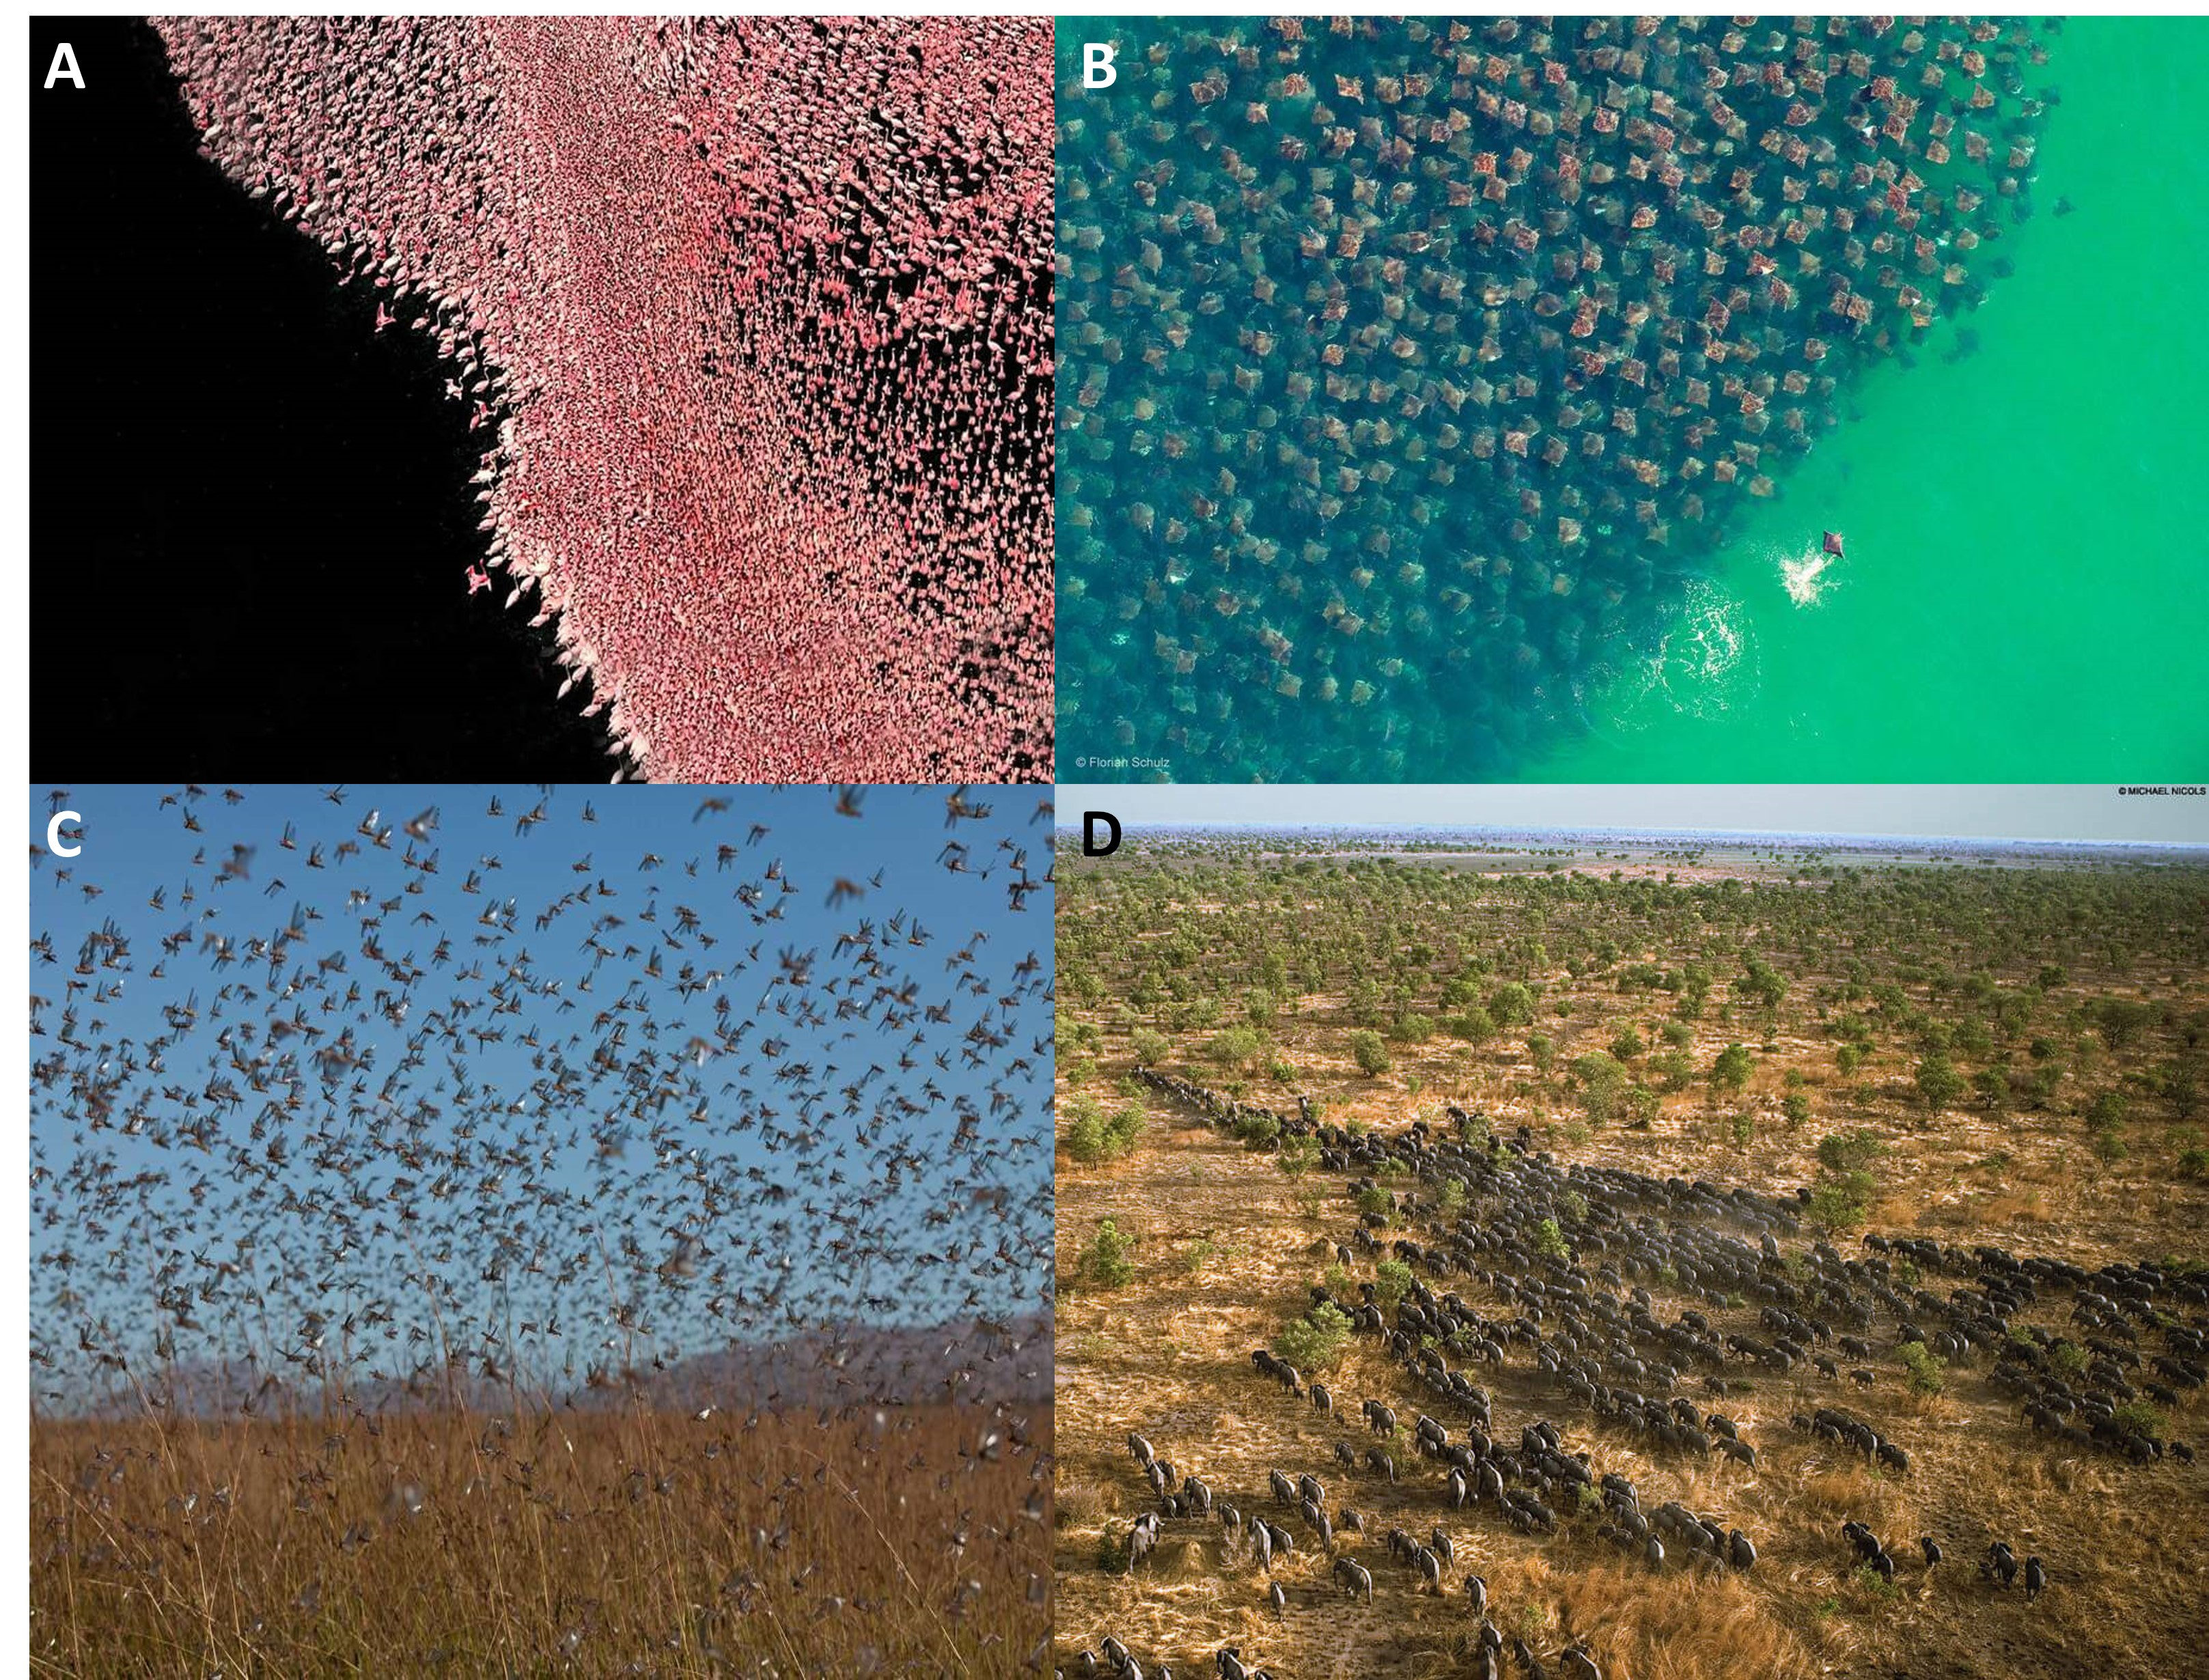
\includegraphics[width=0.85 \textwidth]{Figures/groupes_pdf.jpg}
		\rule{35em}{0.5pt}
	\caption[Group]{Exemples de regroupements sociaux chez différents taxons animaux. \textbf{A}. Flamants roses, Kenya. \textbf{B}. Raies mantas, Golfe de Californie (photo : F. Schulz). \textbf{C}. Criquets, Madagascar. \textbf{D}. Éléphants, Tchad.}
	\label{fig:group}
\end{figure}

%-----------------------------------
%	SUBSECTION 2
%-----------------------------------

    \subsection{Valeur adaptative et coûts}
    \label{subsec:benef}
A première vue, la vie en groupe apporte des inconvénients. Parmi les plus évidents, on peut citer une transmission facilitée des pathogènes entre les individus ou encore le partage inégal d'une ressource entre les membres d'un groupe social \cite{danchin_ecologie_2005}. Malgré tout, ce mode de vie offre de nombreux bénéfices (recensés par \citet{krause_living_2002}). L'un des plus documenté et étudié dans la littérature est une diminution du risque de prédation \cite{vulinec_collective_1990}. Des effets de dilution/confusion sont notamment impliqués et sont caractérisés par une augmentation soudaine de proies pouvant effrayer le prédateur ou diminuer ses chances de capture. Il y a également une augmentation de la vigilance, l'hypothèse de l'effet \textit{many-eyes}. Plus il y a d'individus, plus il y a d'individus-détecteurs diminuant de fait le temps de détection d'un prédateur. Le regroupement d'individus offre également un rapprochement des partenaires sexuels amenant à une augmentation du taux d'accroissement et de reproduction de la population \cite{courchamp_allee_2008}. Cette liste, bien que non exhaustive, montre certains avantages liés à la vie en groupe. Ces avantages vont être pérennisés par le maintien de la cohésion sociale \cite{krause_living_2002}.
    


%-----------------------------------
%	SUBSECTION 3
%-----------------------------------

    \subsection{Classification}
    \label{subsec:classification}
Plusieurs auteurs se sont essayés à classer les différents niveaux d'organisation sociale. \citet{wheeler_social_1928} fut l'un des précurseurs, et c'est à partir de ses observations sur les insectes qu'il classa les niveaux de socialité sur la base du lien entre la mère et sa progéniture. C'est à partir des travaux de Wheeler que Michener, aidé par Wilson, établit une classification hiérarchique des niveaux de socialité (Tableau \ref{tab:classification}). Cette classification, appelée \textit{classification de Michener-Wilson}, reste à ce jour la plus communément utilisée, et notamment en entomologie. Michener et Wilson considèrent une espèce dite \textit{sociale}, comme toute espèce présentant \textit{une communication réciproque de nature coopérative} \citep{michener_social_1974, wilson_insect_1971}. Par communication est entendue ici \textit{toute action individuelle qui influence la probabilité d'apparition d'un comportement chez un autre individu}. Pour résumer, l'eusocialité caractérise le niveau le plus élevé, que l'on retrouve très majoritairement chez les arthropods et notamment les fourmis, les abeilles ou les termites. Ce stade est défini par un chevauchement des générations d'adultes, une coopération pour les soins aux jeunes et une spécialisation d'individus pour la reproduction (Tableau \ref{tab:classification})


\begin{table}[p]
	\caption[Classification]{Classification des différents niveaux de socialité selon Michener et Wilson (cité dans \citet{lihoreau_organisation_2009} et modifié d'après \citet{aron_les_2009}).}
    \centering
	
\includegraphics[width=1 \textwidth]{Figures/classification.png}
		\label{tab:classification}
\end{table}   

\begin{table}[p]
	\caption[Classification2]{Classification des différents niveaux de socialité suite à l'observation des sociétés de vertébrés (tiré de \citet{kerth_group_2010}).}
    \centering
	
\includegraphics[width=0.8 \textwidth]{Figures/classification2.png}
		\label{tab:classification2}
\end{table}      

Bien que critiquée par plusieurs auteurs (critiques résumées par \citet{costa_other_2006}), la classification de Michener-Wilson est largement utilisée dans la littérature scientifique. Une critique fréquente est que ces auteurs se sont basés sur des espèces d'arthropodes, et qu'il était donc difficile de transposer cette classification aux sociétés de vertébrés. Une autre classification tirée de l'observation des groupes de vertébrés a été proposée (Tableau \ref{tab:classification2}; \cite{kerth_group_2010}). Avec cette dernière, les groupes de blattes, les volées d'oiseaux ou encore les larves nécrophages de Diptères sont considérées comme \textit{grégaires}. Des exemples de sociétés de type fission/fusion sont retrouvés chez les éléphants (Figure \ref{fig:group}) ou les dauphins. 

Afin d'éviter toute confusion, les termes de \textit{grégaire}, \textit{social} et \textit{eusocial} seront ici utilisés pour définir les niveaux de socialité, en accord avec la classification de Michener-Wilson.
    
  

%----------------------------------------------------------------------------------------
%	SECTION 2
%----------------------------------------------------------------------------------------
\section{L'agrégation}
\label{sec:agregation}
Le comportement d'agrégation, ou grégarisme, est considéré d'un point de vu évolutif comme le premiers pas vers des niveaux de socialité supérieurs \citep{campan_ethologie._2002, aron_les_2009}. Ce comportement d'inter-attraction entre les individus est indépendant de l'attraction sexuelle. Si on se réfère à la distribution spatiale des organismes, \citet{camazine_self-organization_2001} définissent une agrégation comme un assemblage d'individus qui entraîne une forte densité de ceux-ci dans les environs. Ces groupes trouvent leur origine et leur cohésion par l'inter-attraction de leurs membres, d'où la nécessité qu'il y ait un transfert d'information (i.e. communication) entre les individus constituant ce groupe \citep{camazine_self-organization_2001, ame_collegial_2006}. L'agrégation est généralisée aux sociétés d'invertébrés (Figure \ref{fig:aggregation}) et peut apparaître comme une réponse à des hétérogénéités environnementales (agrégation non sociale) ou à l'attraction entre individus (agrégation sociale \cite{costa_other_2006}). Le grégarisme est l'un des phénomènes sociaux les plus primaires, et beaucoup d'activités d'insectes sociaux lui sont liées, comme les déplacements ou le fourragement \citep{deneubourg_dynamics_2002, simpson_gregarious_2001, wertheim_effects_2006}.


%-----------------------------------
%	SUBSECTION 1
%-----------------------------------

    \subsection{Les différents types d'agrégation}
    \label{subsec:types}
Deux types d'agrégation sont classiquement connus et admis dans la littérature: l'agrégation dite \textit{non sociale} et celle dite \textit{sociale}.

L'agrégation non sociale, ou agrégation résultant de l'habitat selon \citet{danchin_evolution_1997}, n'est qu'apparente car elle est dépendante des facteurs abiotiques. Les individus vont répondre positivement à des hétérogénéités environnementales. Imaginons un habitat où on observe un grand nombre de parcelles pauvres et quelques parcelles riches, et qu'une population répartie de manière \textit{libre idéale} s'y trouve. Libre étant défini par le fait que les individus se déplacent entre les diverses parcelles sans aucun coût ni contraintes et idéale mentionne qu'ils connaissent parfaitement l'environnement. Bien qu'il y ait un rassemblement sur les parcelles riches, cette observation ne fait que refléter la variation de la qualité de l'environnement. Il résulte de la somme des réponses individuelles aux hétérogénéités du milieu. Ces caractéristiques du milieu peuvent jouer un rôle de \textit{template}, un modèle, permettant de prédire le pattern agrégatif final observé \cite{camazine_self-organization_2001}.
Un second exemple d'agrégation non sociale apparaît lorsque les facteurs abiotiques vont déplacer et restreindre les individus dans une zone. Les agrégats de méduses en sont un bon exemple. Par la force des courants marins et des vents en surface, des mouvements de convection amènent à la formation d'agrégats contenant de nombreux individus \cite{hamner_regularly_1986}. 

L'agrégation sociale, qui nous intéresse plus particulièrement dans ce travail, est définie par \citet{vulinec_collective_1990} comme étant \textit{la tendance qu'à un animal à s'agréger avec d'autres de façon à ce qu'il soit en contact l'un de l'autre, ou proche, et que la distribution de ces animaux dans l'environnement local soit extrêmement inégale}\footnotemark[1]\footnotetext[1]{\textit{"the tendency of an animal to aggregate with others such that the animals are in contact with one another, or are nearly so, and that the distribution of the animals in the local environment is extremely patchy}" \cite{vulinec_collective_1990}.}. La constitution de ces groupes implique la présence d'interactions sociales \cite{parrish_animal_1997} à plus ou moins longue portée et basées sur des signaux chimiques, visuels, tactiles ou sonores. Ces agrégations sont variables en terme de durées et de compositions. Des espèces peuvent être regroupées durant toute leur vie, comme les fourmis ou les abeilles, ou seulement à un moment de leur développement comme les larves de Diptères. D'autres exemples de grégarisme chez les arthropodes sont présentés dans l'article de vulgarisation paru dans \textit{Espèces} (cf. Annexe \ref{Annexes2}) co-écrit avec Pierre \textsc{Broly} (Unité d'Ecologie Sociale, ULB).


 \begin{figure}[ht]
	\centering
		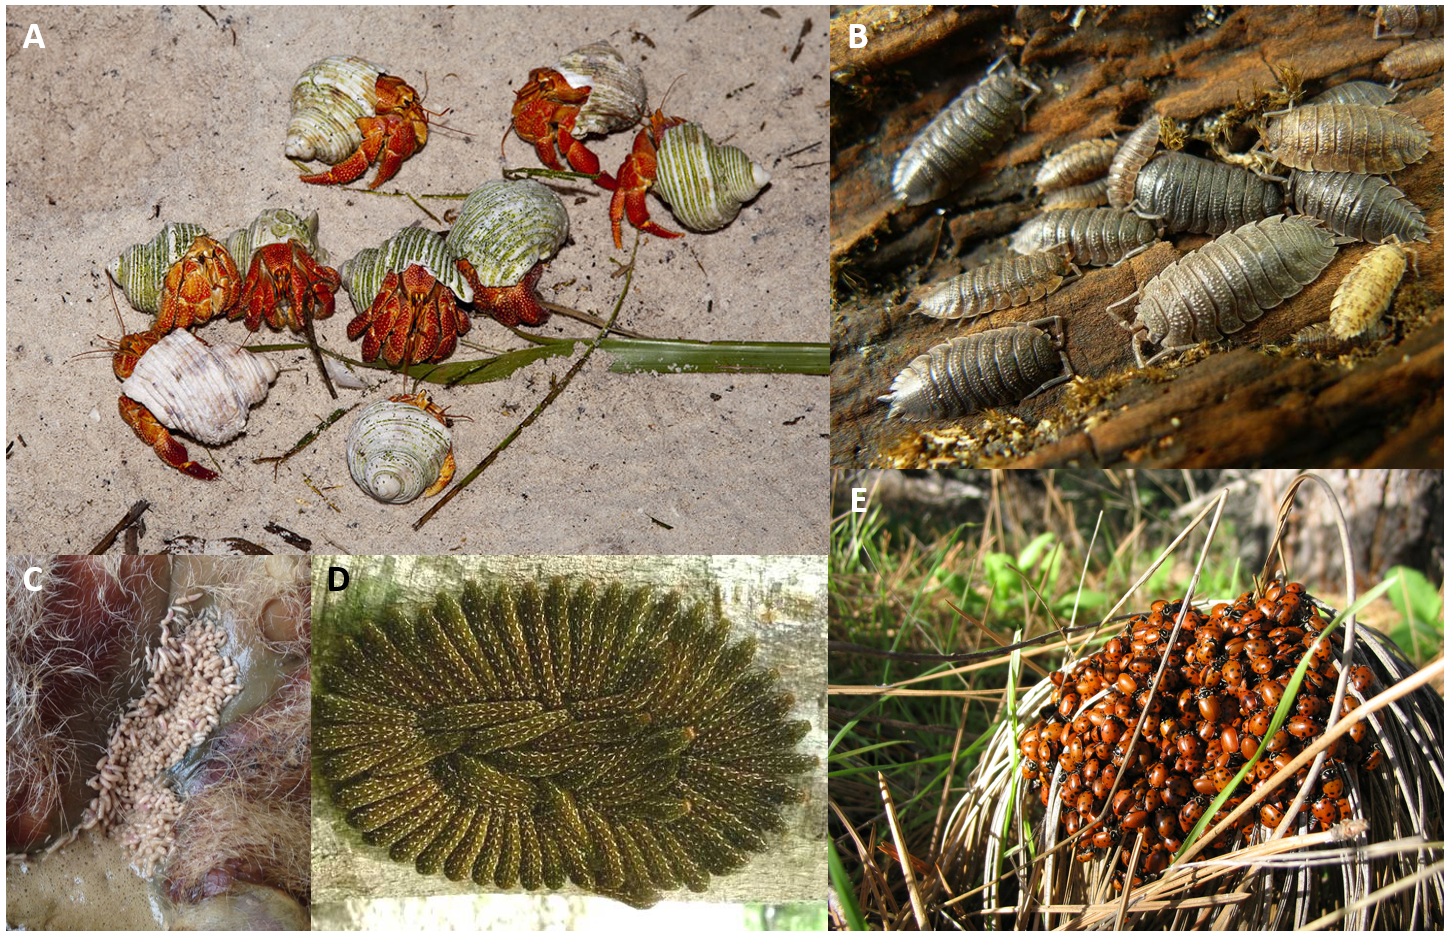
\includegraphics[width=0.9 \textwidth]{Figures/aggregation.png}
		\rule{35em}{0.5pt}
	\caption[Aggregation]{Exemples d'agrégation chez différents taxons d'arthropodes. \textbf{A}. Bernard l'hermite fraise (\textit{Oenobita perlatus} ; photo : K. Marks). \textbf{B}. Cloportes (\textit{Porcelio scaber} ; photo : S. Reekie). \textbf{C}. Larves nécrophages de Diptères (Calliphoridae ; photo : J. Boulay). \textbf{D}. Chenilles du papillon Ruby-spotted Swallowtail (\textit{Papilio anchisiades} ; photo : V. Ciau). \textbf{E}. Coccinelles (\textit{Harmonia axyridis} ; photo : J. Goddard).}
	\label{fig:aggregation}

\end{figure}


%----------------------------------------------------------------------------------------
%	SECTION 3
%----------------------------------------------------------------------------------------

	\section{L'auto-organisation: de l'individuel au collectif}
    \label{sec:autoorganisation}
La notion d'auto-organisation est appliquée en éthologie, en particulier aux insectes sociaux, pour montrer comment un comportement collectif complexe peut émerger à partir d'interactions simples entre individus (Figure \ref{fig:selforga}; \cite{camazine_self-organization_2001}). \citet{bonabeau_auto-organisation_1997} définissent l'auto-organisation comme \textit{les phénomènes au cours desquels une certaine structuration spatiale et/ou temporelle s'opère plus ou moins "spontanément", ou encore sous l'effet d'un flux énergétique, entropique ou matériel}. Cette définition étant issue de la physique \cite{bonabeau_self-organization_1997}, \citet{camazine_self-organization_2001} en distinguent deux grandes différences avec l'auto-organisation appliquée aux systèmes biologiques. La première est la grande complexité des sous-unités des systèmes biologiques. Les sous-unités en physique sont des objets inanimés alors qu'en biologie se sont des organismes vivants complexes. La seconde concerne la nature des lois qui gouvernent les interactions dans ces deux disciplines. Dans les systèmes physico-chimiques, les patterns créés au travers des interactions obéissent uniquement aux lois de la physique. Les systèmes biologiques obéissent également à ces mêmes lois mais les interactions physiologiques et comportementales sont influencées par les propriétés génétiquement contrôlées des composants. \citet{bonabeau_auto-organisation_1997} précisent cette définition dans le cadre des comportements collectifs comme tout \textit{processus au cours duquel des structures émergent au niveau collectif, à partir de la multitude des interactions entre individus, sans être codées explicitement au niveau individuel}. Ces derniers résument l'auto-organisation à trois points essentiels : \textit{(i) l'apparition d'une structure spatio-temporelle ; (ii) cette structure est principalement produite de l'intérieur du système [...] ; (iii) enfin, la notion mal définie qu'une structure "remarquable" "émerge" est traduite par la difficulté voire l'impossibilité pour un observateur [...] de prédire l'apparition de la structure et encore moins ses propriétés}. 

Derrière cette définition, il vient à l'esprit la notion de \textit{complexité} chère à Edgar Morin \cite{morin_methode_1977}. Sumpter \cite{sumpter_principles_2006} relie cette notion à l'auto-organisation avec cette définition : \textit{Le principe central de l'auto-organisation est que les interactions simples répétées entre les individus peuvent produire des modèles adaptatifs complexes au niveau du groupe}\footnotemark[2].\footnotetext[2]{\textit{"The central tenet of self-organization is that simple repeated interactions between individuals can produce complex adaptive patterns at the level of the group."}\cite{sumpter_principles_2006}}  
Dans sa thèse d'HDR, Gautrais \cite{gautrais_dynamiques_2015} critique l'idée que les interactions entre les individus doivent être \textit{simples} tant qu'elles sont \textit{répétées}. Il liste un certains nombre d'exemples d'interactions, allant des réactions chimiques d'oxydo-réduction aux comportements individuels lors de la construction de pistes chez les fourmis, montrant que ces comportements non rien de "simples". Il avance plutôt l'idée que la multitude d'individus présents se comportent de manière \textit{stochastique} et donc non déterministe. Cet élément offre une source de fluctuation qui constitue l'auto-organisation \cite{gautrais_dynamiques_2015}. Gautrais \cite{gautrais_dynamiques_2015} montre également l'importance de \textit{l'amplification} des interactions plus que leur répétition. Il donne ainsi sa propre définition de l'auto-organisation: \textit{"Modèle expliquant le comportement d’ensemble d’un système stochastique par la possibilité que ses fluctuations aléatoires soient amplifiées."}\cite{gautrais_dynamiques_2015}.
Avec cette dernière définition, on voit bien les deux notions essentielles qui constituent l'auto-organisation : \textit{la stochasticité} et \textit{l'amplification}.
L'un des exemples les plus explicites traduisant ces deux notions est le suivi de piste chez la fourmi \cite{deneubourg_collective_1989}. Si on laisse à une colonie le choix entre deux branches d'un même pont strictement identiques allant du nid à une ressource alimentaire, les premières fourmis vont choisir aléatoirement l'une des deux branches du pont. Ces fourmis vont laisser un marquage chimique au sol (dépôt de piste) incitant leurs congénères à emprunter cette branche. Ce premier choix de branche s'est fait de manière stochastique mais le choix des fourmis suivantes s'est vu biaisé en faveur du pont marqué. Ces dernières vont à leur tour marquer de leur passage cette branche peu marquée augmentant un peu plus les probabilités que d'autres fourmis empruntent cette branche du pont. Cet exemple reflète très bien la dynamique de type amplification d'un système stochastique.

 \begin{figure}[ht]
	\centering
		\includegraphics[width=0.8 \textwidth]{Figures/selforga.jpg}
		\rule{35em}{0.5pt}
	\caption[Selforga]{Exemples de structures collectives. \textbf{A}. Banc de sardines (photo: B. Cole). \textbf{B}. Entrée d'un nid de fourmis (\textit{Myrmecia sp.} ; photo : G. Park). \textbf{C}. Mouvement de "Ola" lors d'un match de basketball (photo : Journal Sud Ouest). \textbf{D}. Déplacement collectifs de moutons en Irlande (photo : P. Brennan). \textbf{E}. Nid de termites dans le parc national Litchfield (photo : H. Zaher).}
	\label{fig:selforga}

\end{figure}

%----------------------------------------------------------------------------------------
%	SECTION 4
%----------------------------------------------------------------------------------------

	\section{L'amplification du système}
    \label{sec:amplification}

L'agrégation est une source d'amplification. Une augmentation de la densité d'individus dans une zone accroît de fait la probabilité qu'ont les individus de reproduire une action donnée. Ces mécanismes amplificateurs jouent un rôle déterminant dans l'élaboration des agrégations sociales reposant sur des dynamiques non linéaires \citep{camazine_self-organization_2001, deneubourg_dynamics_2002}.\\  
L'amplification est régie par des boucles rétroactives positives et/ou négatives, appelées \textit{feedbacks}, qui permettent l'accroissement du système mais aussi l'empêchent d'exploser. Un exemple bien connu de feedback positif est le suivi de piste chez les fourmis décrit précédemment (Figure \ref{fig:feedback}). Une fourrageuse dépose une piste chimique allant de la ressource au nid. Ses congénères vont suivre cette piste accroissant sa concentration et ainsi mécaniquement la probabilité que d'autres fourmis suivent cette piste augmente \cite{dussutour_organisation_2004}. Un autre exemple, toujours chez la fourmi, est la probabilité de déposer un cadavre d'une congénères, qui va augmenter avec le nombre de cadavres déjà présents \cite{deneubourg_collective_1989}. La probabilité de quitter un groupe, qui décroit avec le nombre de membres, est un exemple de feedback négatif (Figure \ref{fig:feedback}). A noter qu'avec cet exemple de feedback négatif pairs cela conduit à l'apparition d'un feedback positif (plus d'individus sortent d'un groupe, plus d'individus rejoignent un second groupe). D'autres exemples de feedbacks sont décrits par \citet{jeanson_positive_2009}.\\



 \begin{figure}[ht]
	\centering
		
\includegraphics[width=0.9 \textwidth]{Figures/feedback.png}
		\rule{35em}{0.5pt}
	\caption[Feedback]{Exemples de boucles rétroactive positives (+) chez les fourmis et négatives (-) chez les blattes (tiré de \citet{jeanson_positive_2009}).}
	\label{fig:feedback}   
 \end{figure}   
 
%----------------------------------------------------------------------------------------
%	SECTION 5
%----------------------------------------------------------------------------------------
	\section{La prise de décision collective}
    \label{sec:decision}
La prise de décision collective, \textit{collective decision-making}, joue un rôle central dans la vie des animaux sociaux. Les humains en sont un bon exemple avec les élections dans les démocraties. Selon \citet{conradt_consensus_2005} cette décision, souvent appelé abusivement \textit{l'intelligence collective} par le grand public, peut être de deux formes. La première est la \textit{combined decision}, que \citet{conradt_consensus_2005} définissent comme \textit{un choix individuel des membres du groupe (mais pas nécessairement indépendamment) entre deux ou plusieurs actions. Ils ne visent pas un consensus mais les résultats combinés de leurs décisions affectent généralement le groupe dans son ensemble}\footnotemark[3]. Ces auteurs présentent quelques exemples de telles décisions comme l'allocation de tâches chez les insectes eusociaux ou des décisions liées à la consommation chez l'humain. L'individu choisit seul sans chercher un consensus mais son comportement est dépendant de celui du groupe auquel il appartient.

Le second type de décision collective, celui qui nous intéresse dans ce travail, est la décision consensuelle, \textit{consensus decision}, (Figure \ref{fig:consensus}) qui apparaît lorsque \textit{les membres d'un groupe choisissent entre deux ou plusieurs actions mutuellement exclusives dans le but spécifique de parvenir à un consensus}\footnotemark[4] \cite{conradt_consensus_2005}. Les exemples avancés par \citet{conradt_consensus_2005} peuvent être la coordination des prédateurs pour l'attaque d'une proie ou encore le choix d'une destination lors d'un trajet. \citet{conradt_consensus_2005} ont ensuite établi une classification des décisions consensuelles (Figure \ref{fig:consensus}) selon qu'il y ait, ou non, un conflit d'intérêt puis la présence d'une communication globale ou locale. Une communication globale étant définie comme une communication simultanée entre tous les membres du groupe, à la différence de celle locale, où seulement les individus proches peuvent communiquer \cite{conradt_consensus_2005}. Dans le cas des larves nécrophages de Diptères, les individus ont une perception limitée de leur environnement, laissant penser à l'existence d'une communication locale des membres au sein du groupe.

 

\footnotetext[3]{\textbf{Combined decision}: members of a group choose individually (but not necessarily independently) between two or more actions. They do not aim for
consensus but the combined results of their decisions usually affect the group
as a whole.}
\footnotetext[4]{\textbf{Consensus decision}: members of a group choose between two or more mutually exclusive actions with the specific aim of reaching a consensus.}

    
 \begin{figure}[ht]
	\centering
		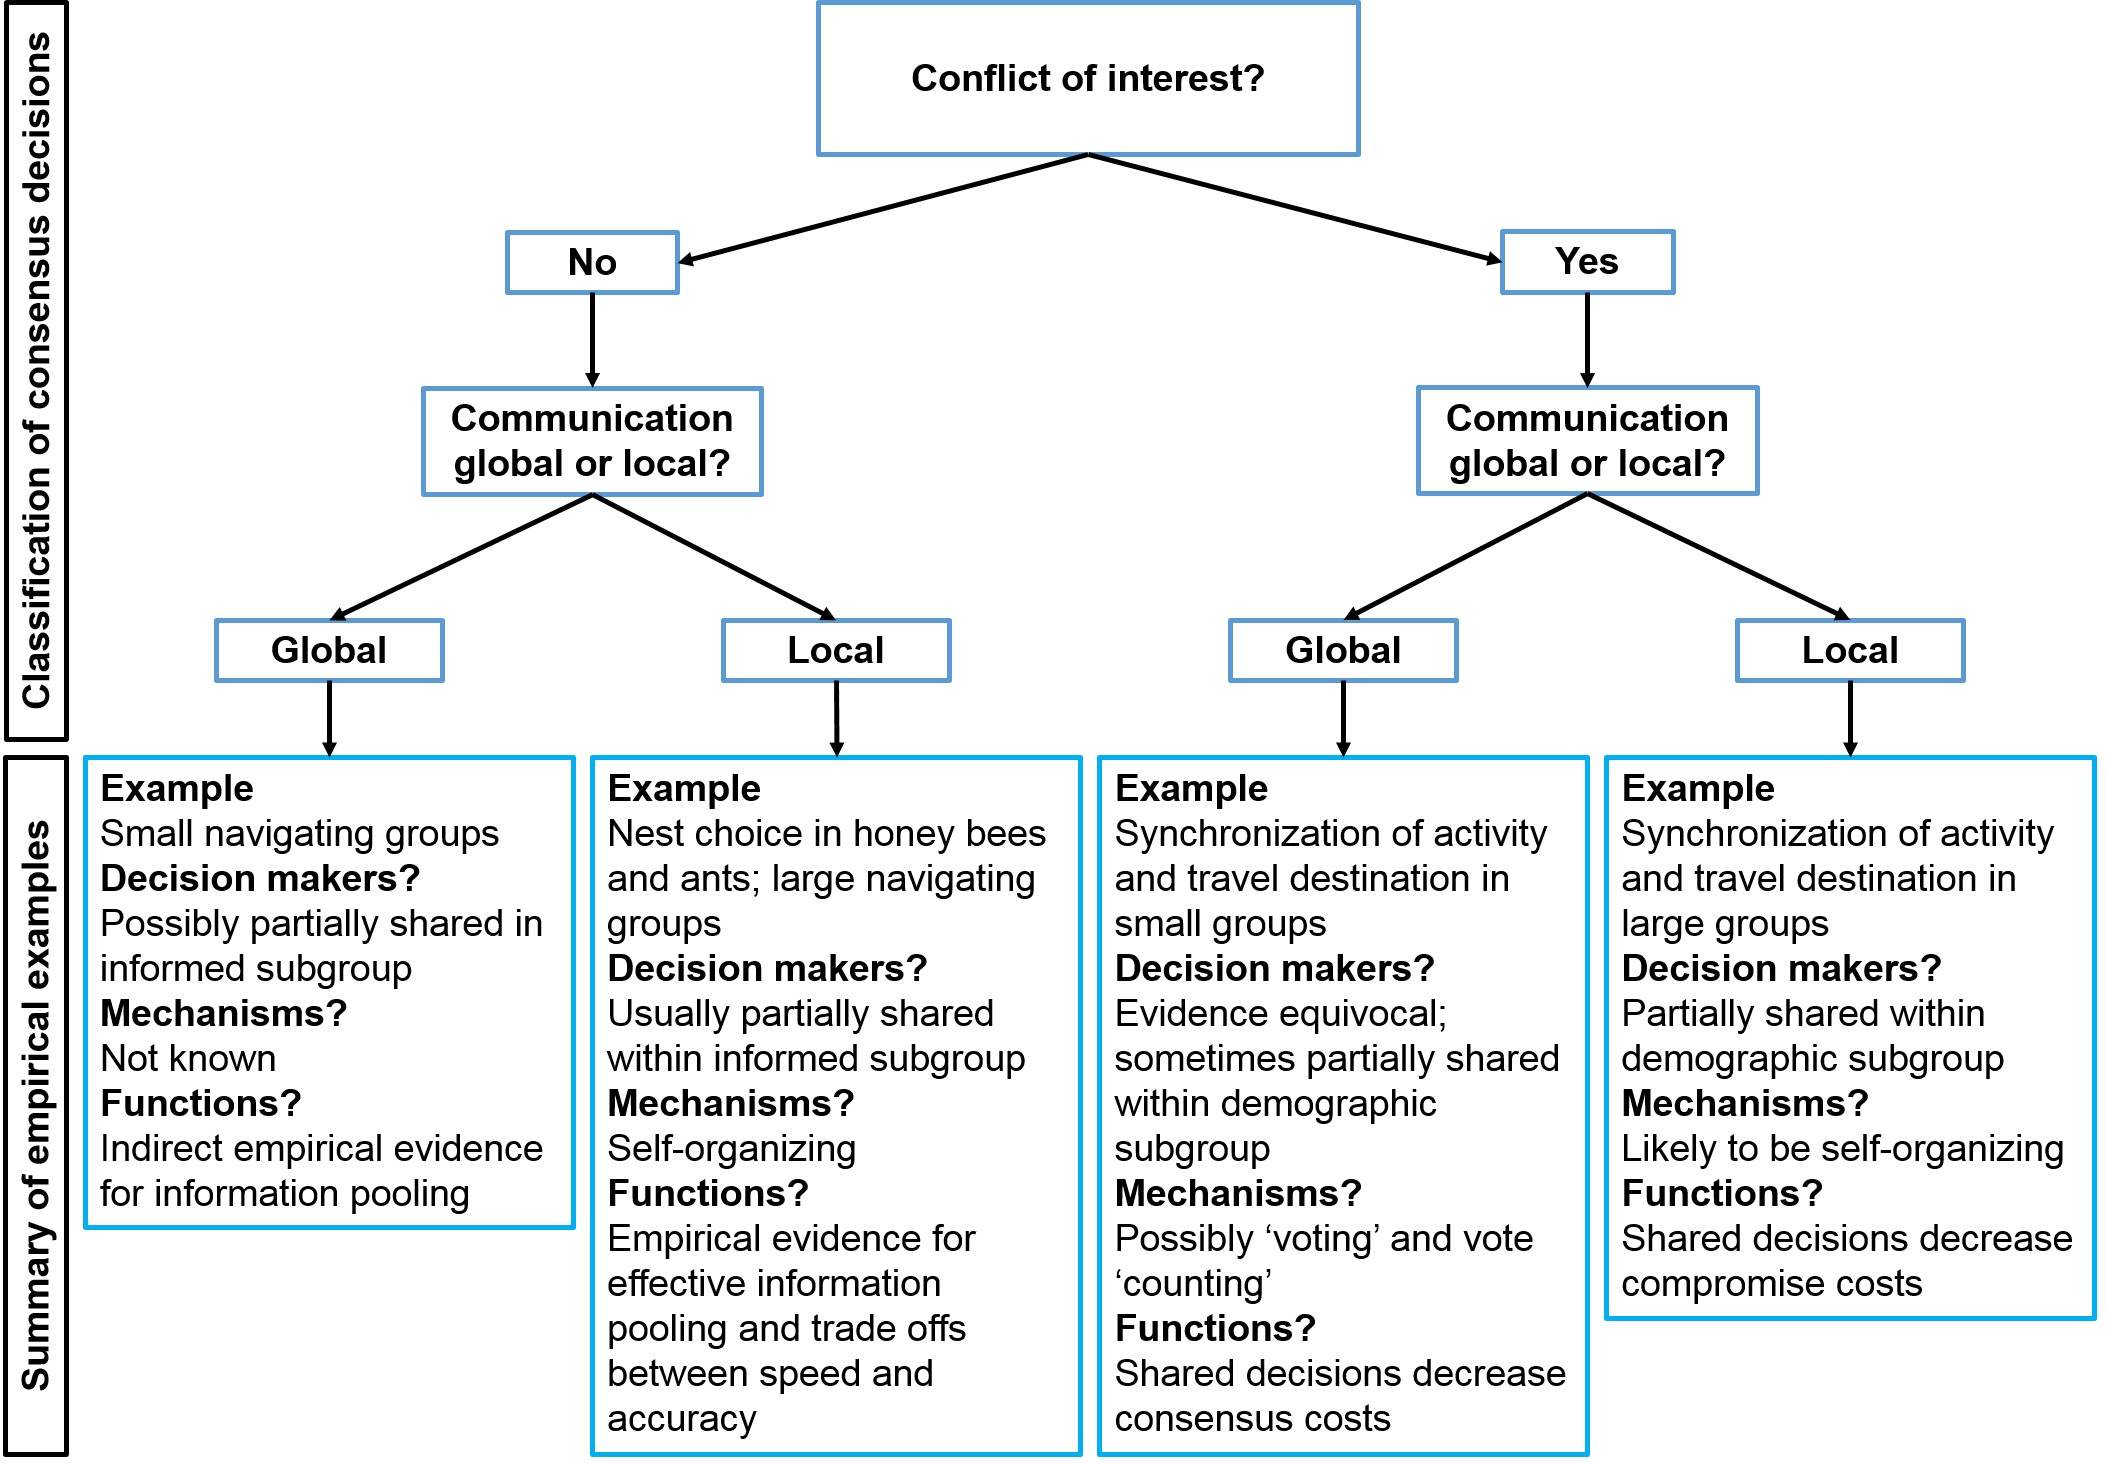
\includegraphics[width=0.8 \textwidth]{Figures/consensusdecision.png}
		\rule{35em}{0.5pt}
	\caption[Consensus]{Vue schématique de la classification actuelle des décisions consensuelles, \textit{consensus decisions} (tiré de \citet{conradt_consensus_2005}).}
	\label{fig:consensus}   
 \end{figure}       

\clearpage
%----------------------------------------------------------------------------------------
%	SECTION 6
%----------------------------------------------------------------------------------------

\section{Les insectes nécrophages}


%-----------------------------------
%	SUBSECTION 1
%-----------------------------------

	\subsection{L'écosystème cadavre et rôle des insectes}
Par définition, le cadavre est une ressource instable et éphémère. Ce biotope, à haute valeur énergétique, apparaît de façon imprédictible, d'où la nécessité pour les espèces nécrophages, i.e. qui se nourrissent des cadavres, de le détecter et de s'y rendre rapidement. C'est un environnement hétérogène avec différentes gammes de températures ainsi que des spots de nourriture à valeur nutritionnelle inégale (e.g. foie, cerveau etc.) \cite{ireland_effects_2006}.

Les insectes nécrophages sont les principaux artisans de la décomposition d'un cadavre \citep{marchenko_medico-legal_1988, payne_summer_1965}. En s'alimentant, ils vont contribuer de manière significative à augmenter la vitesse de dégradation du cadavre (Figure \ref{fig:degradation}, \cite{payne_summer_1965}). On trouve principalement parmi eux des espèces de Diptères et de Coléoptères.   

\begin{figure}[ht]
\centering
		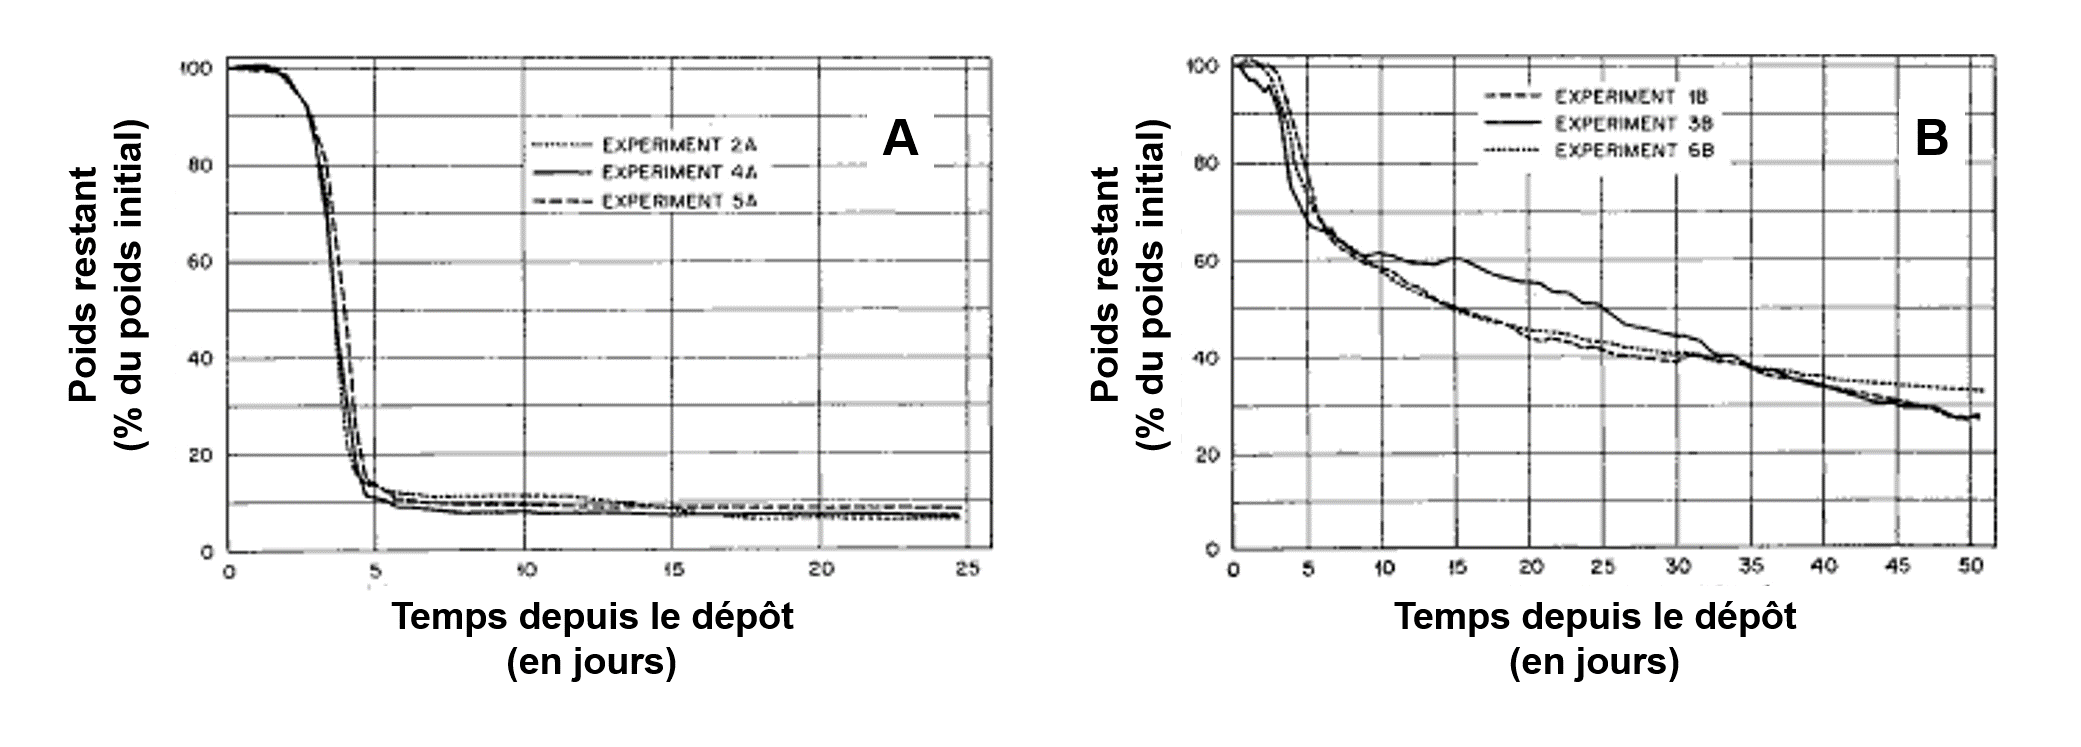
\includegraphics[width=0.85 \textwidth]{Figures/degradation.png}
		\rule{35em}{0.5pt}
		\caption[Degradation]{Évolution temporelle de la masse de porcelets (\textit{Sus scrofa}) en présence \textbf{A} et en absence \textbf{B} d'insectes nécrophages (tiré de \citet{payne_summer_1965}).}
	\label{fig:degradation}
\end{figure}


%-----------------------------------
%	SUBSECTION 2
%-----------------------------------

    \subsection{Les insectes pionniers : les Diptères Calliphoridae et Sarcophagidae}
Les insectes pionniers que l'on retrouve sur les cadavres en décomposition appartiennent principalement aux Calliphoridae et Sarcophagidae. Ces insectes sont dotés d'organes sensoriels très sensibles leurs permettant de détecter un corps à plusieurs kilomètres de distance \cite{barton_browne_role_1960}. Cette détection se fait dès quelques heures après la mort via la perception des composés volatils relargués par le cadavre \cite{frederickx_responses_2012}. Le cadavre va servir de substrat de ponte et de ressource alimentaire pour leurs larves, appelées couramment asticots.

		\subsubsection{Cycle de développement}
Les Diptères nécrophages sont des insectes holométaboles, c'est-à-dire à métamorphose complète. Leur cycle de développement est composé de 4 stades : œuf, larve, pupe et adulte (Figure \ref{fig:cycle}). La durée de ce cycle est dépendante de deux paramètres : l'espèce et la température. Plus la température ambiante est élevée, plus la durée du cycle de développement est courte (et inversement). De plus, à température identique, des individus vont se développer plus ou moins rapidement selon l'espèce à laquelle ils appartiennent.

La femelle pond ses œufs, préférentiellement au niveau des orifices naturels du corps (Figure \ref{fig:pontes}). Ces œufs sont pondus en paquets d'environ 200 et sont généralement agrégés avec ceux d'autres femelles \citep{fenton_oviposition_1999, brodie_is_2014}. Cette agrégation des pontes est la résultante de signaux attractifs comme la présence d'œufs, de larves et/ou d'adultes. Les femelles vont chercher un site de ponte à la fois humide, évitant ainsi la dessiccation des larves, et permettant pour leur progéniture un accès facile à la nourriture.
Après l'éclosion, les larves vont passer par trois stades (L1, L2 et L3) entrecoupés par deux mues. Puis, le stade pré-pupe, qui est un stade intermédiaire entre L3 et pupe, et qui correspond, chez la plupart des espèces, à la phase d'éloignement du corps. Ensuite, la larve pré-pupe se transforme en pupe (i.e. cocon), d'où émergera un imago (Figure \ref{fig:cycle}).   

\begin{figure}[ht]
\centering
		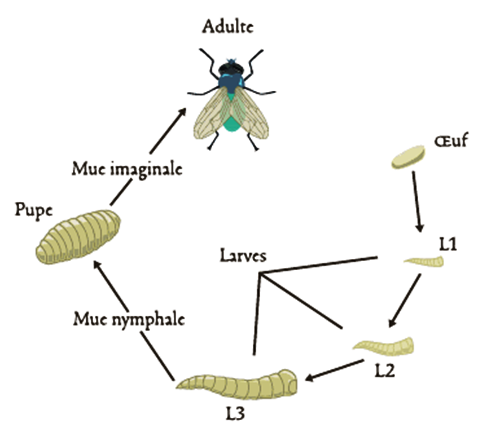
\includegraphics[width=0.6 \textwidth]{Figures/cycle_d_veloppement.png}
		\rule{35em}{0.5pt}
		\caption[Cycle]{Cycle de développement des Diptères Calliphoridae (schéma : J. Boulay ; Infographie: \textit{Espèces}). A 25\up{o}C, la durée de ce cycle pour \textit{Lucilia sericata} est de 13 jours alors que pour \textit{Calliphora vicina} elle est de 17 jours \cite{marchenko_medico-legal_1988}.}
	\label{fig:cycle}
\end{figure}

\begin{figure}[ht]
\centering
		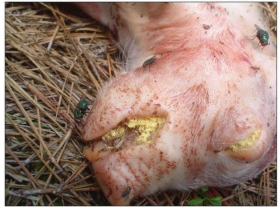
\includegraphics[width=0.8 \textwidth]{Figures/pontes.pdf}
		\rule{35em}{0.5pt}
		\caption[Pontes]{Pontes agrégées de femelles de Diptères Calliphoridae sur un cadavre de porcelet (photo : Edward B. Mondor).}
	\label{fig:pontes}
\end{figure}
 
        \subsubsection{Importance des Diptères en entomologie forensique}
        \label{subsubsec:forensique}
L'entomologie forensique est l'étude des insectes dans le contexte d'enquêtes judiciaires. Les bases de cette science ont été posées par Jean-Pierre Mégnin en 1894 dans son ouvrage \textit{La Faune des cadavres}. Il est le premier à avoir décrit les différentes successions d'insectes nécrophages sur un cadavre, qu'il a appelé \textit{escouades}. Ces travaux ont montré que les Diptères Calliphoridae font parti des premiers insectes à arriver sur le cadavre.

Ces insectes, dont les durées de développement en fonction de l'espèce et de la température sont bien connues, vont permettre de définir une datation du décès \cite{charabidze_insectes_2014}. Cette datation se fait après identification des insectes et connaissant l'historique thermique du lieu où ces espèces se sont développées. 

Avec toutes ces informations, l'expert entomologiste va pouvoir établir une chronologie débutant par l'arrivée des insectes jusqu'à la découverte du corps (Figure \ref{fig:ipm}). Il faut bien garder à l'esprit que l'expert donne un Intervalle Post-Mortem minimum (IPMmin) et non la date effective de la mort. En effet, suivant l'accessibilité du cadavre et les conditions climatiques, les insectes vont mettre un certain temps à arriver et à pondre sur celui-ci. Un corps retrouvé dans les bois sera rapidement colonisé, et donc un IPMmin proche de la date du décès, en comparaison d'un corps retrouvé dans un coffre de voiture. De même, les conditions climatiques comme le froid ou la pluie vont fortement réduire l'activité des insectes \cite{voss_decomposition_2007}.

Les insectes nécrophages peuvent aussi être utilisés comme matrice pour des dosages toxicologiques, on parle alors d'\textit{entomo-toxicologie}. On peut également les utiliser pour détecter des traces de poudre dues à l'utilisation d'une arme à feu. 

A l'heure actuelle, la physiologie de ces insectes est bien connue alors que les études comportementales font défaut. L'importance des Diptères dans le cadre d'expertise renforce l'idée qu'il est nécessaire d'étudier le comportement de ces insectes. Ces recherches comportementales pourraient permettre \textit{in fine} d'affiner les techniques de datation existantes.

\begin{figure}[ht]
\centering
		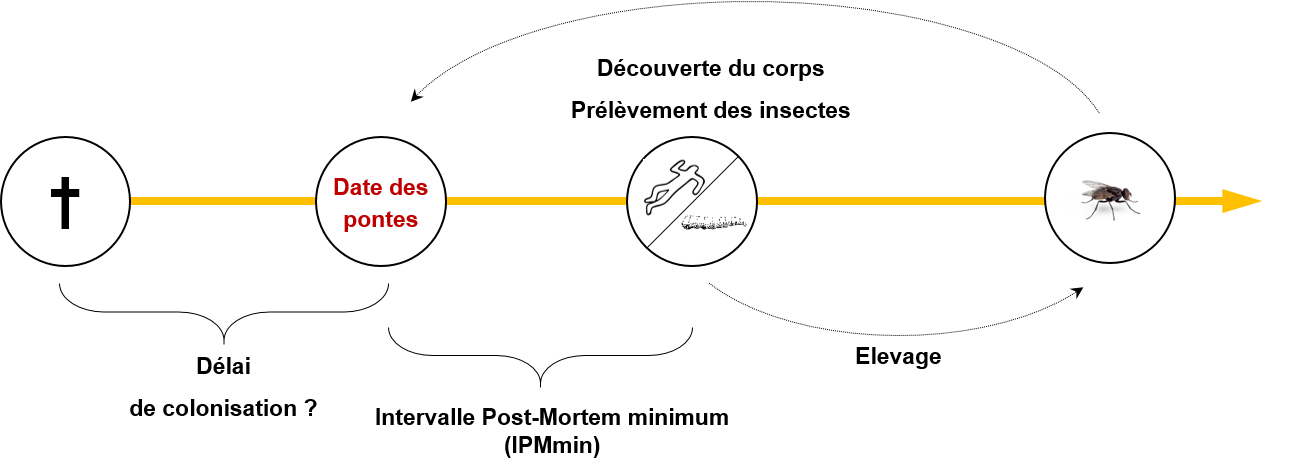
\includegraphics[width=0.9 \textwidth]{Figures/IPM.png}
		\rule{35em}{0.5pt}
		\caption[IPM]{Chronologie d'une expertise entomologique du décès. Le délai de colonisation va être impacté par l'accessibilité du corps et des conditions climatiques. La partie élevage se fait en laboratoire en conditions de température et de nourriture contrôlées.}
	\label{fig:ipm}
\end{figure}


%-----------------------------------
%	SUBSECTION 3
%-----------------------------------
 
\subsection{Description du modèle biologique}

Cette thèse s'est essentiellement focalisée sur deux espèces de Diptères Calliphoridae, \textit{Lucilia sericata} (Meigen, 1826) et \textit{Calliphora vomitoria} (Linné, 1758) (Figure \ref{fig:mouche}). L'espèce \textit{Calliphora vicina} (Robineau-Desvoidy, 1830) a été utilisée seulement pour une étude (cf. Chapitre \ref{Chapter5}). Ces espèces sont présentes dans toutes les régions tempérées et tropicales du monde. 

\begin{figure}[ht]
	\centering	
        \begin{subfigure}{0.25\textwidth}
			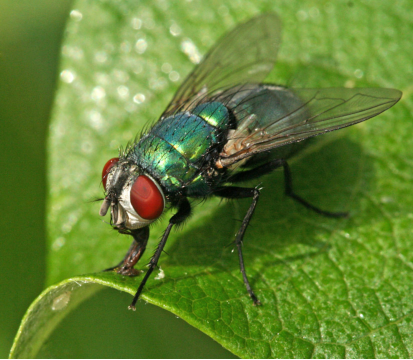
\includegraphics[width=\linewidth]{Figures/210509alf537luciliaw.pdf}
			\caption{\textit{Lucilia sericata}}
				\label{sub:lucilia}
		\end{subfigure}
		\begin{subfigure}{0.265\textwidth}
			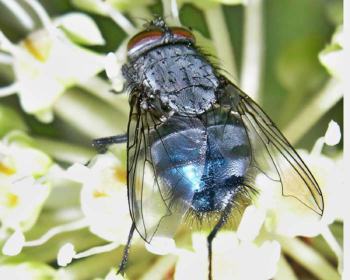
\includegraphics[width=\linewidth]{Figures/Calliphora-vomitoria-03.pdf}
			\caption{\textit{Calliphora vomitoria}}
				\label{sub:calliphora}
		\end{subfigure}
        \begin{subfigure}{0.29\textwidth}
			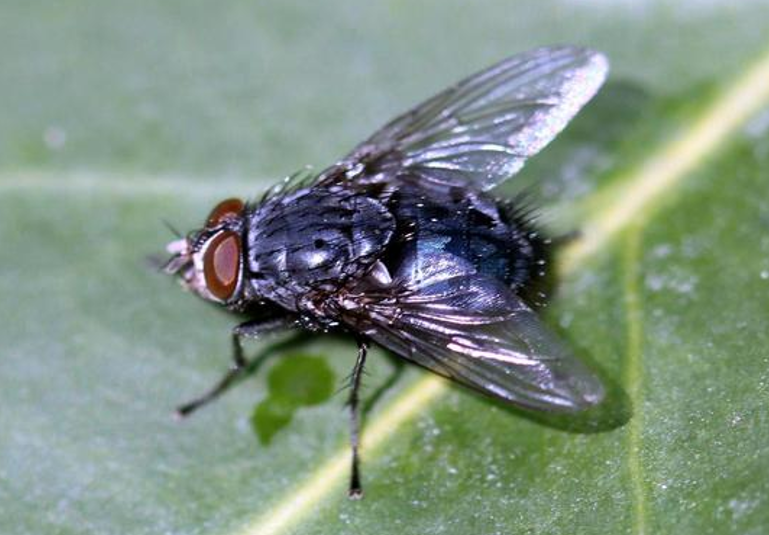
\includegraphics[width=\linewidth]{Figures/vicina.png}
			\caption{\textit{Calliphora vicina}}
				\label{sub:calliphoravic}
		\end{subfigure}
		\rule{35em}{0.5pt}
        \caption[Species]{La mouche verte (\textbf{A}) et les mouches bleues (\textbf{B} et \textbf{C}), les espèces utilisées lors de ce travail.}		
			\label{fig:mouche}
	\end{figure}

    
    \subsubsection{Anatomie}
		\label{subsubsec:anatomie}
Les larves nécrophages de Diptères disposent de deux crochets buccaux antérieurs utilisés pour l'alimentation (Figure \ref{fig:organes}). Dans cette même région, deux organes sensoriels présents en paire sont présents : l'organe dorsal (\textit{Dorsal Organ (DO)}), utilisé pour l'olfaction \cite{chu-wang_fine_1971-1} et l'organe terminal (\textit{Terminal Organ (TO)}) utilisé pour la gustation \cite{chu-wang_fine_1971} (Figure \ref{fig:organes}). Les larves disposent également de 12 photorécepteurs regroupés sous le nom \textit{d'organe de Bolwig} \cite{hinnemann_see_2010}. Cet organe détecte la lumière sur un spectre allant de 400 à 630nm \cite{hinnemann_see_2010}. La Figure \ref{fig:organes} a été obtenue en photographiant une larve L3 de \textit{Lucilia sericata} avec un Microscope Électronique à Balayage Environnemental (MEBE). Cet appareil permet de photographier le sujet sans passer par une étape de métallisation des tissus comme utilisée par \citet{colwell_preparation_1986}.  

Sur la partie postérieure, des stigmates sont présents permettant aux larves de respirer (Figure \ref{fig:stigmates}). L'emplacement, non intuitif pour un humain, de ces stigmates permet aux larves de respirer tout en se nourrissant sur le cadavre. Après chaque mue, une fente s'ajoute à celles déjà présentes (stade L1, stigmate à une fente ; stade L2, stigmates à deux fentes et stade L3, stigmates à trois fentes). Cette caractéristique permet de distinguer facilement le stade de développement de la larve observée.

\begin{figure}[p]
\centering
		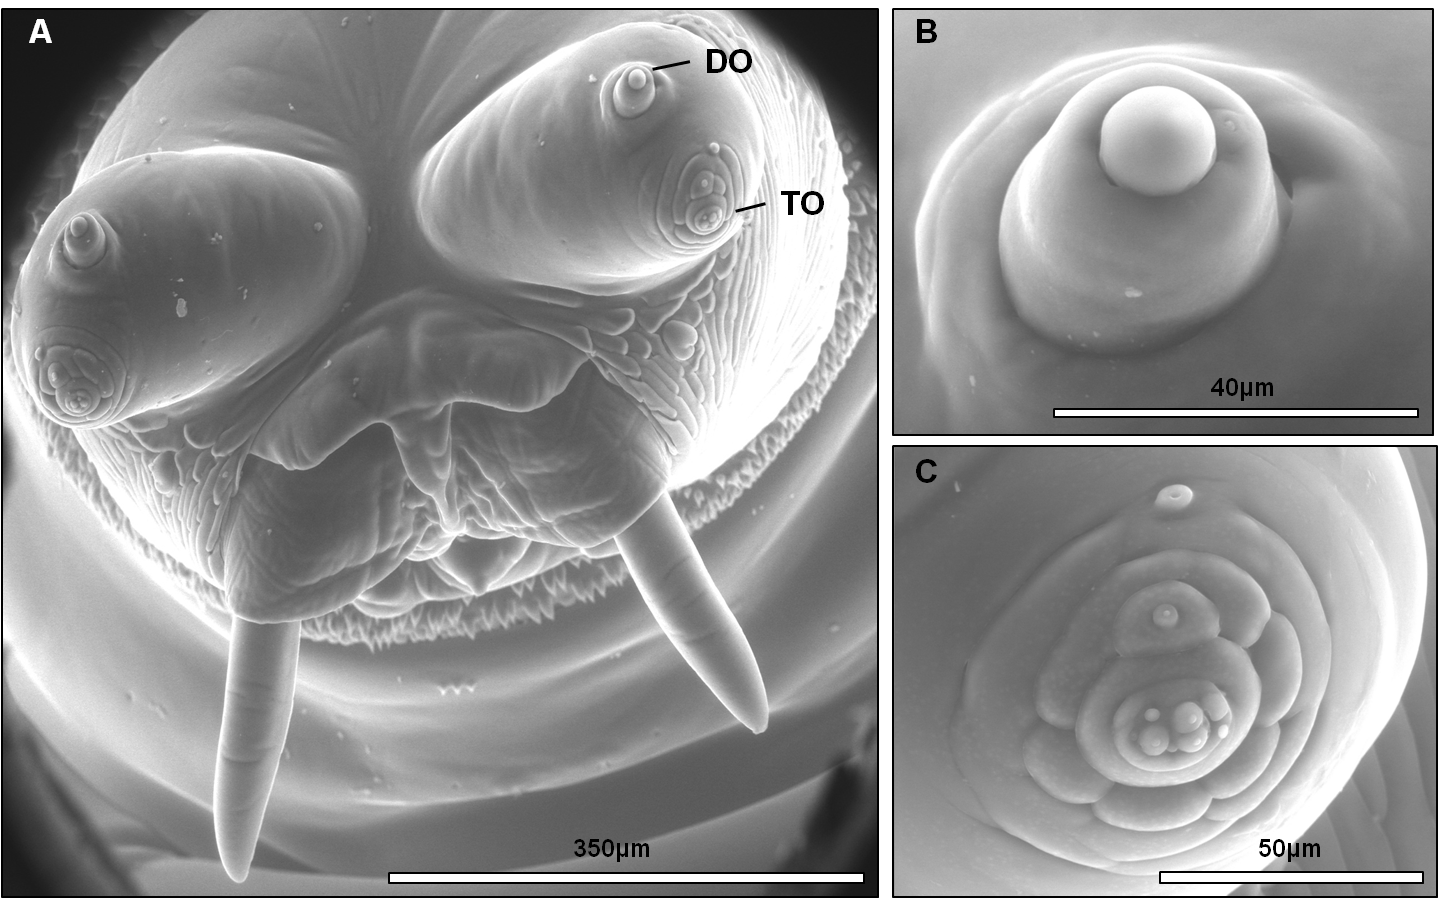
\includegraphics[width=0.9 \textwidth]{Figures/organes.png}
		\rule{35em}{0.5pt}
		\caption[Organes]{Organes sensoriels d'une larve de \textit{Lucilia sericata} observés au microscope électronique à balayage environnemental (MEBE). \textbf{A}. Tête de la larve avec la présence des crochets buccaux. \textbf{B}. \textit{Dorsal organ (DO)} utilisé pour l'olfaction. \textbf{C}. \textit{Terminal Organ (TO)} utilisé pour la gustation (photos : J. Boulay avec l'aide de Lucile \textsc{Géant} (Technicienne au Laboratoire d'Analyses Physiques et de Caractérisation des Matériaux, Douai)).}
	\label{fig:organes}
\end{figure}

\begin{figure}[ht]
\centering
		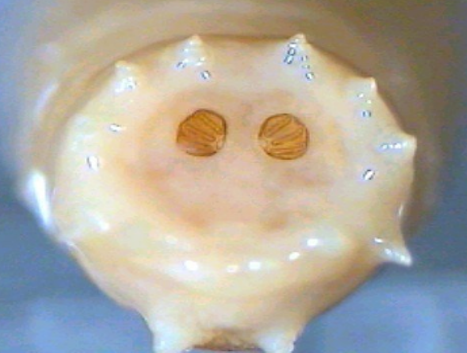
\includegraphics[width=0.7 \textwidth]{Figures/stigmates.png}
		\rule{35em}{0.5pt}
		\caption[Stigmates]{Vue postérieure d’une larve de \textit{Calliphora vicina}
(Diptera : Calliphoridae) au stade L3. Les fentes des stigmates postérieurs permettent de déterminer rapidement le stade de l’individu : 1 fente par stigmate au stade L1, 2 au stade L2 et 3 au stade L3 (photo : B. Bourel).}
	\label{fig:stigmates}
\end{figure}
\clearpage

    \subsubsection{Comportement}
Cette section est issue du Chapitre \textit{Comportement et développement des larves nécrophages} présent dans le livre \textit{Insectes, cadavres et scènes de crime} (Édition: De Boeck ; Éditeurs: D. \textsc{Charabidzé} et M. \textsc{Gosselin}) et écrit en collaboration étroite avec Cindy \textsc{Aubernon} et Damien \textsc{Charabidzé}.


\blockquote{Sur un corps en décomposition, il est fréquent d’observer des masses de larves de Diptères pouvant compter plusieurs centaines à plusieurs milliers d’individus. Les larves qui composent ces masses vont rester en contact physique (agrégat) et se nourrir au même endroit sur le cadavre \cite{rivers_physiological_2011}.}

\blockquote{Du fait de ce comportement grégaire très prononcé, les larves sont en constante bousculade (\textit{scramble competition}) au sein des agrégats. Cette intense activité génère un dégagement de chaleur métabolique pouvant atteindre plusieurs dizaines de degrés (Figure \ref{fig:mass}). Plus la quantité de larve est importante, plus le dégagement de chaleur est élevé \cite{charabidze_larval-mass_2011}. Cette augmentation de température est propice au développement des larves puisqu’elle permet de diminuer sa durée et de ce fait, le temps passé sur le cadavre, limitant ainsi les risques de prédation. Une augmentation trop importante de la température risquerait cependant de tuer les larves. Il existe donc des feedbacks négatifs qui jouent le rôle de régulateurs. Ces régulateurs sont généralement des contraintes physiques et environnementales (Figure \ref{fig:schema}). Chez \textit{L. sericata}, il parait probable que l’accès à la nourriture ainsi que la température locale soient deux facteurs impliqués dans la régulation de la densité et de la localisation des agrégats larvaires \cite{charabidze_larval-mass_2011}.}

\blockquote{Outre le dégagement de chaleur, \citet{rivers_physiological_2011} mettent en avant plusieurs bénéfices liés à l’agrégation (Figure \ref{fig:schema}). Le premier est une coopération pour la digestion. En effet, les larves ont une digestion dite extracorporelle : elles sécrètent une salive riche en antibiotiques et en enzymes protéolytiques qui permettent de liquéfier les tissus \citep{sandeman_tryptic_1990, padilha_sequence_2009}. Plus il y a de larves, plus la quantité de sécrétions salivaires est importante, aboutissant ainsi à une liquéfaction facilitée
des tissus et donc une meilleure assimilation \cite{rivers_physiological_2011}. Un autre bénéfice fréquemment cité est la diminution du risque de prédation. Cette stratégie d’évitement des prédateurs n’a cependant pas été étudiée chez les larves nécrophages de Diptères. Il est enfin probable que l’agrégation limite les pertes d’eau des individus et les protège contre la dessiccation.}

\blockquote{Parallèlement à ces bénéfices, \citet{rivers_physiological_2011}) avancent trois effets délétères majeurs dus à l’agrégation chez les larves de Diptères nécrophages (Figure \ref{fig:schema}. La production de chaleur au sein de l’agrégat peut aboutir à un stress thermique compromettant le développement normal des larves. \citet{wertheim_pheromone-mediated_2005} ont également mis en évidence une chemoattraction des prédateurs et des parasitoïdes, attirés par l’odeur des masses de larves. Enfin, la problématique majeure du grégarisme est la surpopulation au sein des agrégats.
La ponte des femelles étant stimulée par différents signaux attractifs (présence d'œufs, de larves), il y a dans un premier temps agrégation des œufs \cite{esser_factors_1990}. Lorsque les jeunes larves écloses, elles sont donc déjà agrégées sur certaines zones du corps, notamment au niveau des orifices naturels. Au fur et à mesure du développement, la masse larvaire augmente en volume et consomme les ressources. L’appauvrissement des ressources et l’accumulation des déjections (ammoniaque) peut alors compromettre le développement des larves. \citet{kuusela_community_1983} et \citet{prinkkila_complex_1995} démontrent par exemple un effet négatif de la compétition (forte densité larvaire) sur le développement des larves de \textit{Lucilia}. Cependant l’effet contraire, c’est-à-dire une augmentation de la vitesse de développement lorsque la densité augmente, a été décrit chez \textit{Calliphora vicina} \cite{saunders_effects_2013} et \textit{Calliphora vomitoria} \citep{kaneshrajah_calliphora_2004, ireland_effects_2006}. Bien que de tels effets de la densité de larves existent en conditions naturelles et doivent être gardés à l’esprit, il est rare dans un contexte forensique que le cadavre soit une ressource limitante pour les larves de Diptères Calliphoridae. La compétition (hors prédation) est donc généralement faible et n’a alors que peu d’effets sur le développement des larves et l’estimation de l’intervalle post-mortem.}


\begin{figure}[ht]
\centering
		\begin{subfigure}{0.4\textwidth}
			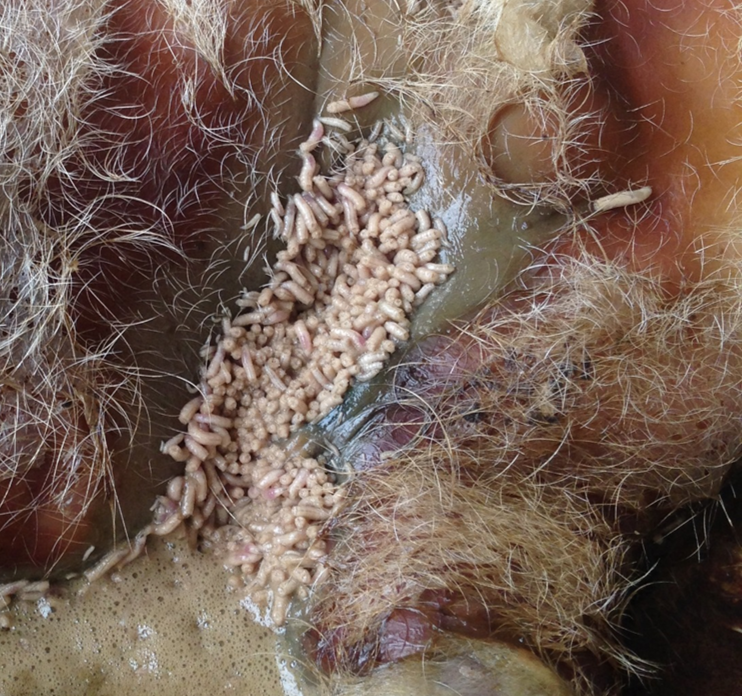
\includegraphics[width=\linewidth]{Figures/mass2.png}
			\caption{Masse larvaire}
				\label{sub:mass2}
		\end{subfigure}
		\begin{subfigure}{0.5\textwidth}
			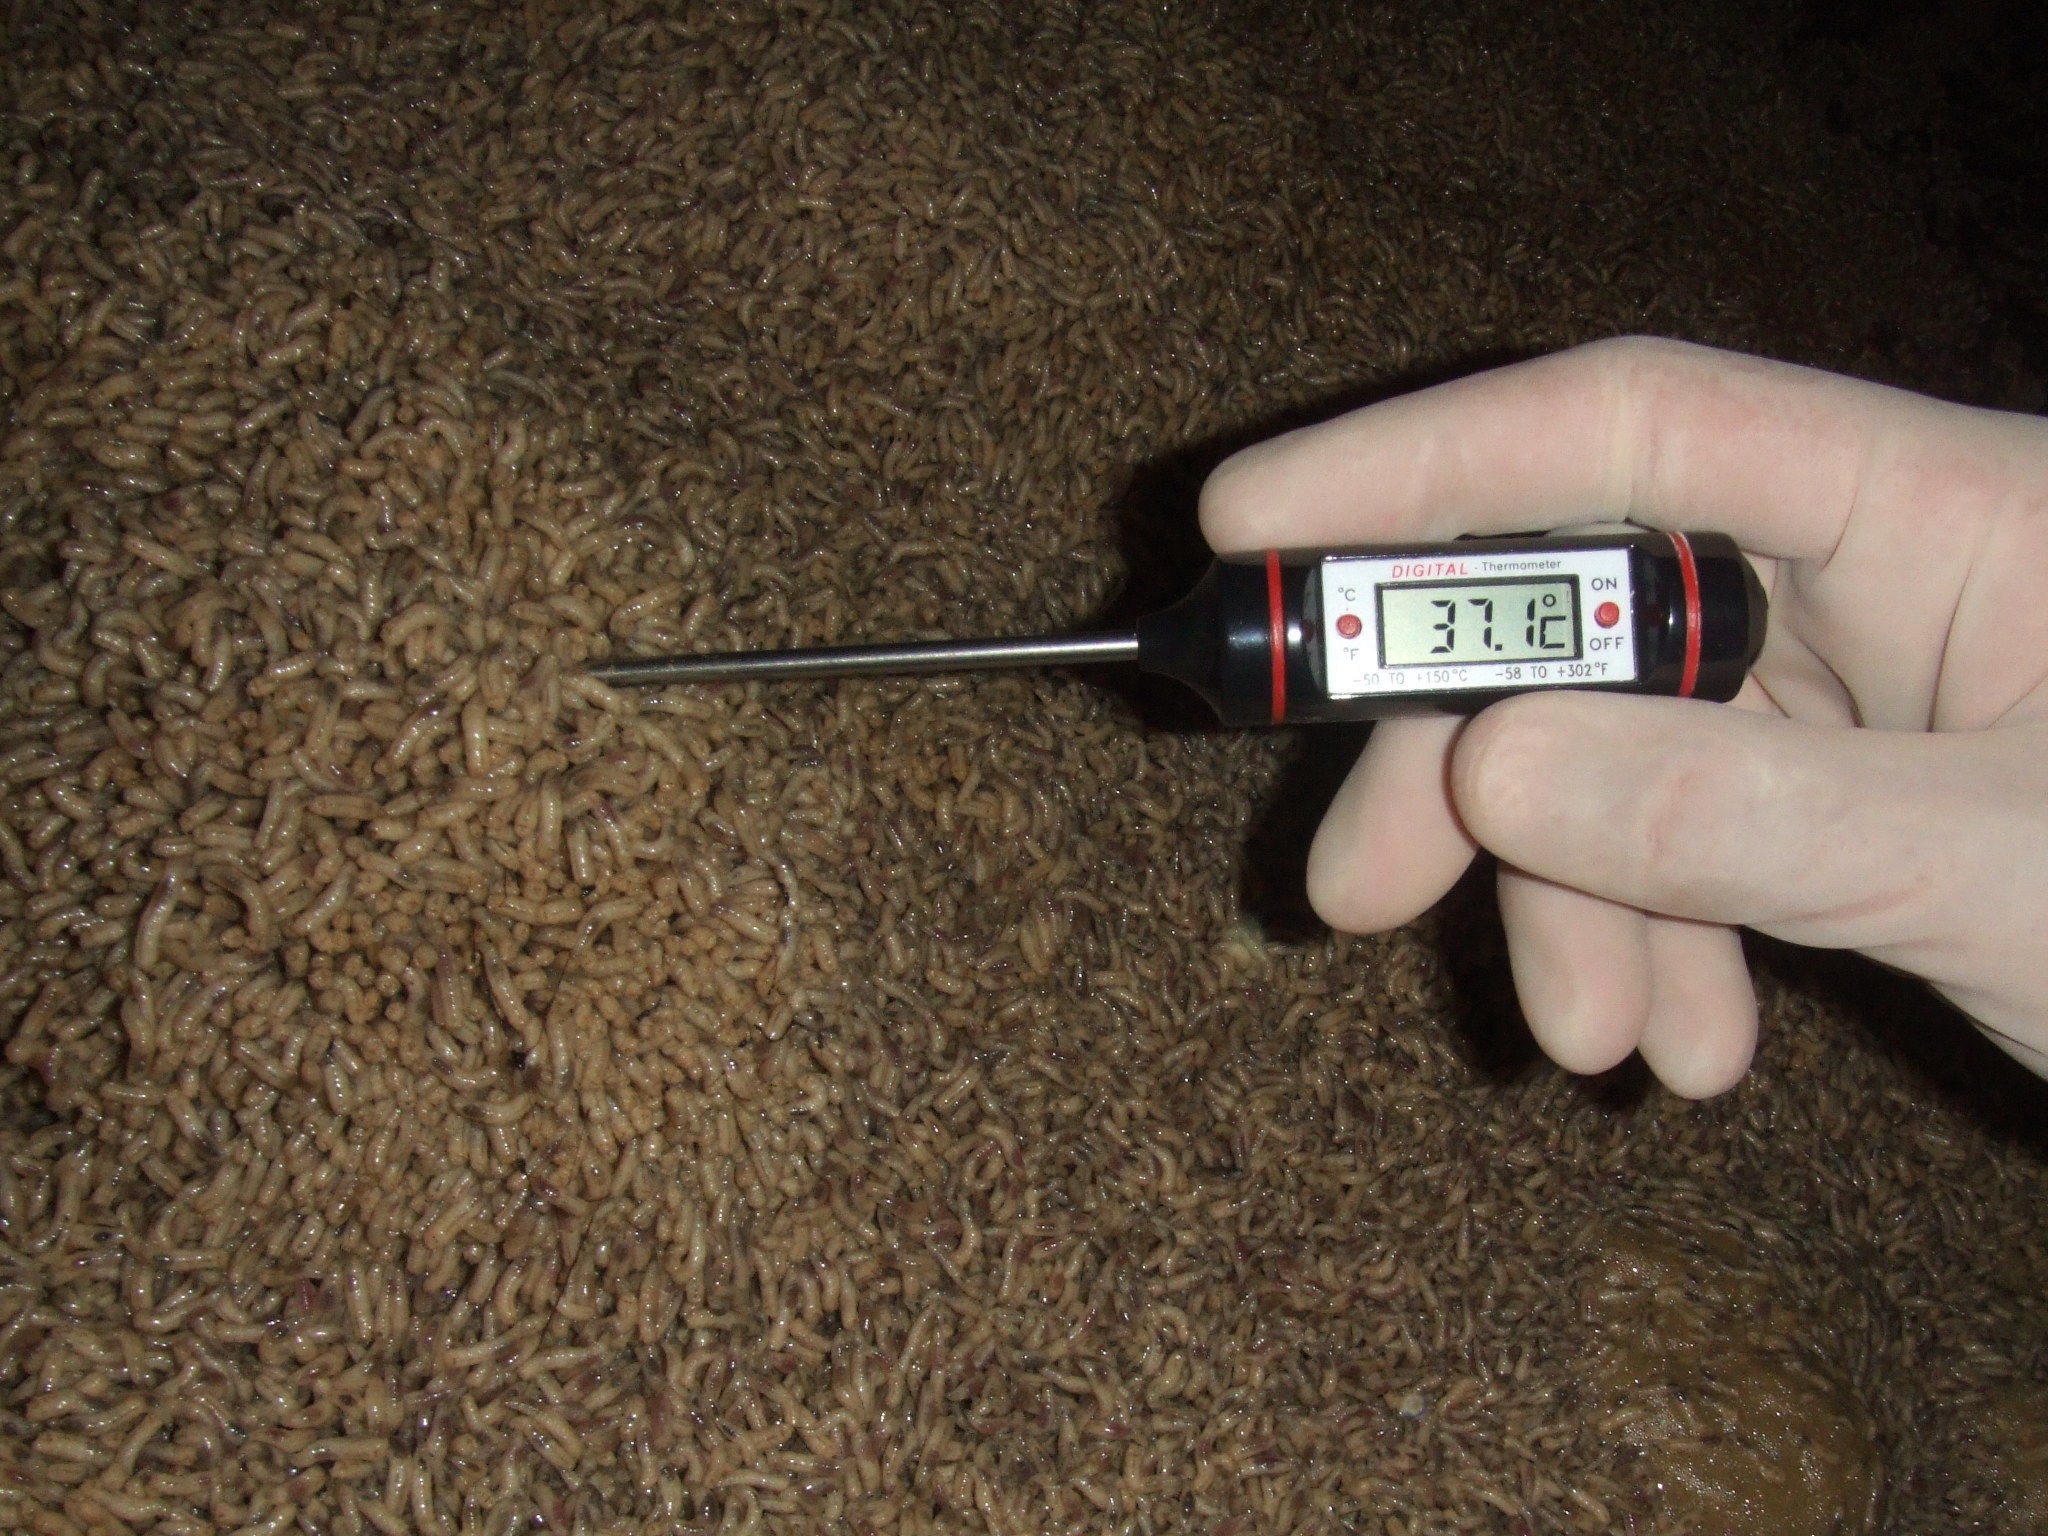
\includegraphics[width= \textwidth]{Figures/larvalmass.JPG}
			\caption[Larval mass]{Larval-mass effect}
		\end{subfigure}
    \rule{35em}{0.5pt}
    \caption{\textbf{A}. Masse larvaire sur un cadavre de porc (\textit{Sus Scrofa} ; photo : J. Boulay). \textbf{B}. Génération de chaleur au sein d’une masse de larves de Calliphoridae (\textit{larval-mass effect}). Cette augmentation locale de la température est positivement corrélée au nombre d’individus présent au sein de la
masse. Cette chaleur accélère le développement des larves, diminuant ainsi le temps passé sur le cadavre en décomposition (photo : D. Charabidzé).}
    \label{fig:mass}
\end{figure}

\begin{figure}[ht]
\centering
		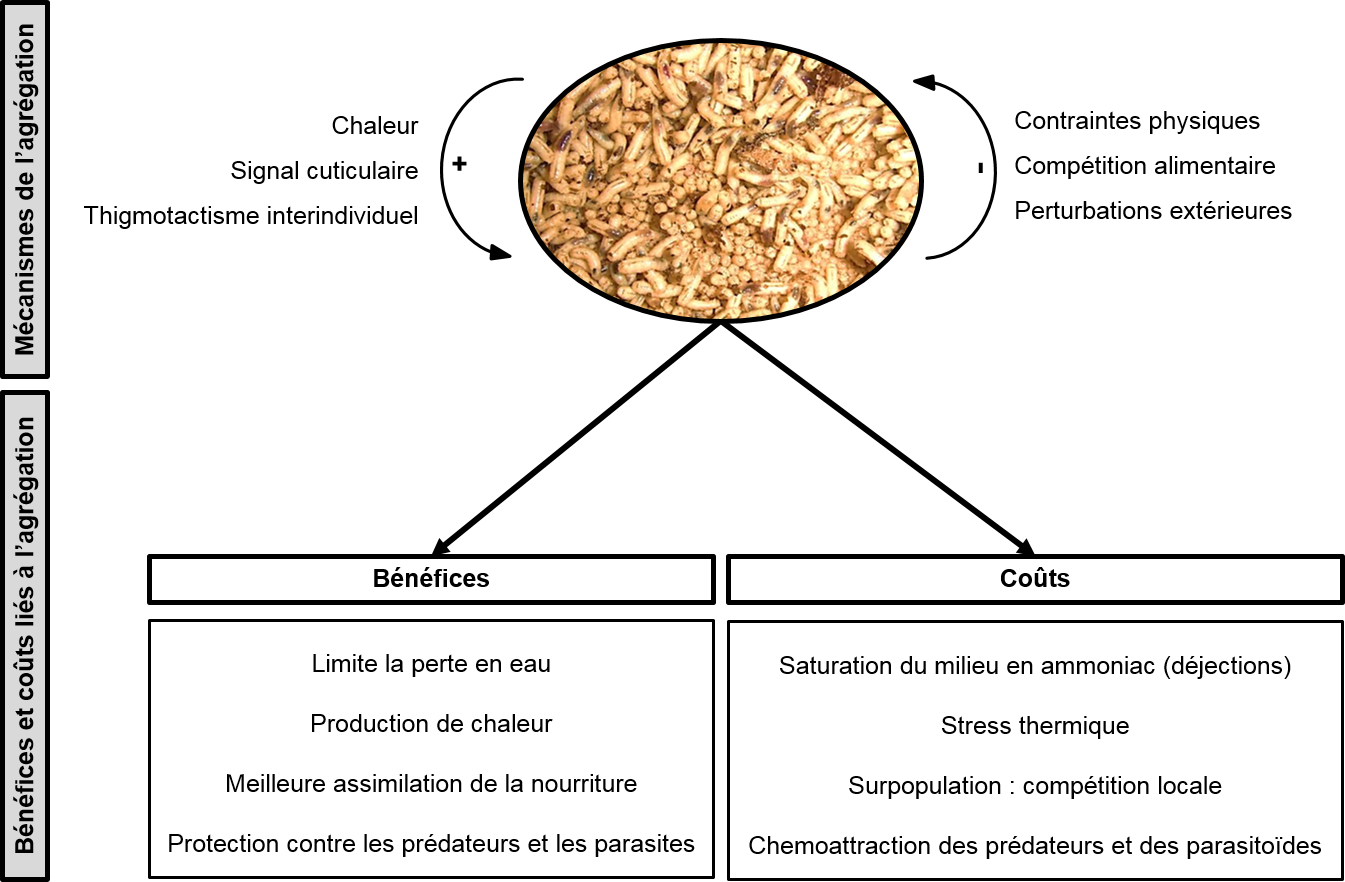
\includegraphics[width=0.9 \textwidth]{Figures/schema.png}
		\rule{35em}{0.5pt}
		\caption[Schema]{Schéma récapitulatif des bénéfices et des effets
délétères liés à l’agrégation ainsi que des mécanismes permettant l’initiation, l’amplification et la régulation du groupe chez les larves grégaires de Calliphoridae et de Sarcophagidae \\ (schéma: J. Boulay).}
	\label{fig:schema}
\end{figure}

\clearpage
% Chapter Template

\chapter*{Objectifs et plan de la thèse} % Main chapter title
\addcontentsline{toc}{chapter}{Objectifs et plan de la thèse}
\label{Methodo} % Change X to a consecutive number; for referencing this chapter elsewhere, use \ref{ChapterX}

\lhead{\emph{Objectifs et Méthodologie générale}} % Change X to a consecutive number; this is for the header on each page - perhaps a shortened title

\textit{``Comme symbole d'effronterie et d'impertinence, il faudrait prendre la mouche. Tandis que tous les animaux, en effet, craignent l'homme au-dessus de tout et le fuient déjà de loin, la mouche, elle, se pose sur son nez."}

\begin{flushright}
Arthur Schopenhauer (1788-1860)
\end{flushright}

\cleardoublepage

%----------------------------------------------------------------------------------------
%	SECTION 1
%----------------------------------------------------------------------------------------

	\section{Objectifs}
Cette thèse a pour objectifs de mettre en évidence et de quantifier les dynamiques d’agrégation des larves nécrophages de Diptères et les mécanismes qui sous tendent ces regroupements. Elle s'inscrit dans deux contextes bien distincts : un fondamental qui est l'étude des comportements collectifs et le second, que l'on peut qualifier d'applicatif, qui est l'entomologie forensique. Bien que le côté théorique soit le plus présent dans cette thèse, l'éventuel apport applicatif de ce travail en contexte judiciaire ne doit pas être négligé.

Comme présentée précédemment dans l'Introduction générale, l'étude de l'agrégation existe chez de nombreux taxons animaux, et en particulier chez les insectes. A l'heure actuelle, aucune étude de ce type n'a cependant été réalisée sur les larves nécrophages de Diptères. Ces insectes ont un comportement d'agrégation très marqué, ayant pour conséquence une forte modification de leur environnement (e.g. génération de chaleur ou production d'enzymes). Les agrégats formés sont, sur un même cadavre, composés de plusieurs espèces.

Les Diptères (e.g. les mouches) sont, à l'heure actuelle, les principaux insectes étudiés et utilisés pour la datation du décès \cite{charabidze_insectes_2014}. Les durées de développement de ces insectes ont été largement étudiées, permettant ainsi d'affiner les techniques de datation utilisées par les experts. En revanche, le comportement des insectes reste mal connu et peu étudié. Cette thèse a pour objectif d'étudier le comportement des Diptères, et plus spécifiquement celui de leurs larves. Ce travail offre une vision comportementale inédite de ces espèces d'intérêt forensique, qui s'ajoutera à une vision physiologique déjà bien établie.

De part ces observations \textit{in natura}, les larves nécrophages sont un modèle d'étude inédit et pertinent dans ce double contexte d'étude (i.e. comportements collectifs et forensique).




%----------------------------------------------------------------------------------------
%	SECTION 2
%----------------------------------------------------------------------------------------

    \section{Plan}

Cette thèse comporte cinq chapitres correspondant chacun à un article publié (cf. Chapitres \ref{Chapter2}, \ref{Chapter3}, \ref{Chapter4}) ou soumis (cf. Chapitres \ref{Chapter1}, \ref{Chapter5}) dans une revue internationale à comité de lecture.

Le premier chapitre est une revue de la littérature (ARTICLE 1) sur les groupes hétérospécifiques chez les arthropodes. Cette revue recense les articles où les auteurs ont observé, décrit ou étudié des groupes hétérospécifiques d'arthropodes dans le contexte de l'étude des comportements collectifs. L'écriture de cette revue fait suite à la constatation de l'absence d'une telle synthèse chez ce groupe animal. L'existence de tels groupes dans la nature remet quelque peu en cause la définition commune de \textit{l'agrégation}. Ils posent également des questions sur la frontière entre les phénomènes de coopération et de compétition entre les espèces. Ces groupes nous offrent un angle d'étude particulièrement intéressant sur ces phénomènes et notamment sur le processus de spéciation sympatrique.

\begin{itemize} 
\item[\tiny{$\blacksquare$}] ARTICLE 1 - Mixed-species aggregation in arthropods - a review\\ (\textbf{soumis} à \textit{Behavioral Ecology}).
\end{itemize}

Le second chapitre (ARTICLE 2) traite de la mise en évidence du comportement actif d'agrégation des larves de \textit{Lucilia sericata} (Diptera: Calliphoridae) sur un milieu nutritif homogène. Cet article démontre l'existence d'un signal déposé au sol par les larves et reconnu par leurs congénères.

\begin{itemize} 
\item[\tiny{$\blacksquare$}] ARTICLE 2 - Evidence of active aggregation behaviour in \textit{Lucilia sericata} larvae and possible implication of a conspecific mark (\textbf{publié} dans \textit{Animal Behaviour}).
\end{itemize}


Le troisième chapitre (ARTICLE 3) s'attache à décrire et quantifier un comportement exploratoire caractéristique des larves nécrophages : le \textit{scanning}. Ce comportement avait été jusqu'alors associé à la recherche de nourriture. Cette étude montre que le scanning est également impliqué dans la recherche de congénères. De plus, ce travail met en évidence les capacités de suivi de trace des larves de \textit{L. sericata}.

\begin{itemize} 
\item[\tiny{$\blacksquare$}] ARTICLE 3 - A first insight in the scanning behaviour of presocial blow fly larvae\\ (\textbf{publié} dans \textit{Physiological Entomology}).
\end{itemize}

Le quatrième chapitre (ARTICLE 4) met en évidence la prise de décision collective chez deux espèces de larves, \textit{L. sericata} et \textit{Calliphora vomitoria}. Ces espèces sont capables de choisir collectivement un site d'agrégation et ce, qu'elles appartiennent à un groupe monospécifique ou hétérospécifique. Cette étude est la première, à notre connaissance, à quantifier la dynamique d'agrégation d'un groupe hétérospécifique d'insectes.

\begin{itemize} 
\item[\tiny{$\blacksquare$}] ARTICLE 4 - Interspecific shared collective decision-making in two forensically important species (\textbf{resoumis} à \textit{Proceedings of the Royal Society of London B}).
\end{itemize}

Le cinquième chapitre (ARTICLE 5) démontre le choix collectif des larves pour une température. Nous avons démontré l'existence de préférendum thermique spécifique chez les larves nécrophages. Sur un gradient de température, les larves sélectionnent collectivement une température selon l'espèce à laquelle elles appartiennent.

\begin{itemize} 
\item[\tiny{$\blacksquare$}] ARTICLE 5 - Thermoregulation in gregarious Dipteran larvae: evidence of species-specific temperature selection (\textbf{soumis} à \textit{Entomologia Experimentalis et Applicata}).
\end{itemize}

Enfin, ce travail s'achève avec une Discussion, qui s'attache à replacer ces travaux dans un contexte évolutif plus large. Elle apporte des perspectives de travail sur l'agrégation des larves nécrophages et la portée plus générale de ces études.

Dans une envie de clarté et de continuité, les références bibliographiques de ce travail (format numéroté) ont toutes été listées en fin de manuscrit (cf. Bibliographie générale). Ce choix assigne à une référence bibliographique un numéro unique pour tout le document. 

\clearpage


    
% Chapter 1

\chapter{Mixed-species aggregation in arthropods - a review} % Main chapter title

\label{Chapter1} % For referencing the chapter elsewhere, use \ref{Chapter1} 

\lhead{Chapitre 1. \emph{Mixed-species aggregation in arthropods - a review}} % This is for the header on each page - perhaps a shortened title

Julien \textsc{Boulay}\up{a,b}, Valéry \textsc{Hédouin}\up{a} and Damien \textsc{Charabidzé}\up{a}

\up{a} Univ. Lille, CHU Lille, EA 7367 - UTML - Unité de Taphonomie Médico-Légale, Lille, France\\
\up{b} Université Libre de Bruxelles, Unit of Social Ecology, Brussels, Belgium\\


Article soumis à \emph{Behavioral Ecology}.


\cleardoublepage

%----------------------------------------------------------------------------------------
%	SECTION 1
%----------------------------------------------------------------------------------------
	\section{Lay summary}
Mixed-species groups are found in a large range of taxa. We reviewed the original research on mixed-species groups and collective behavior in arthropods and highlight the tools that have been used to study and quantify this type of aggregation. The existence of such groups raises questions about the evolution of sociality in animals and the mechanisms involved in cross-species recognition. Finally, this review questions how individuals aggregate with closely related species and the benefits of such groupings. 

	\section{Abstract}
In nature, mixed-species groups are commonly found in mammals and birds, and they have been studied in a collective behavior context. Such mixed-species groups are also observed in a large range of arthropod taxa independent of their level of sociality. Here, we offer the first synthesis of the research on mixed-species groupings in arthropods and highlight the behavioral and evolutionary questions raised by such behavior. As non-mixed (monospecific) groupings provide benefits to individuals, the advantages offered by groupings are described and discussed. These advantages can be attributed to the increase in group size and could be considered to be identical to those of non-mixed groupings (e.g., protection against predators). Furthermore, the competition-cooperation phenomena that might be involved between the species in a group are examined as are the metrics and models commonly used to study heterospecific groups of animals. Several examples are presented to highlight the mechanisms underlying such groupings, particularly the evidence for phylogenetic proximity between members. The study of mixed-species groups offers biologists an interesting way to explore the frontiers of cooperation-competition, especially the process of sympatric speciation.

\textit{Keywords}: complex system, collective behavior, cross-species recognition, self-organization, sociality.

\clearpage

%----------------------------------------------------------------------------------------
%	SECTION 2
%----------------------------------------------------------------------------------------
	\section{Background}
Over the last 40 years, the research on collective behavior has rapidly expanded. In a milestone book entitled \textit{Living in Groups}, Krause and Ruxton \cite{krause_living_2002} reviewed the concepts underlying group living. They focused their work on the mechanisms that govern the evolution and maintenance of animal groups in several species. In 2010, \citet{sumpter_collective_2009} reviewed how the mechanisms driving group behavior are intertwined with understanding its functions; indeed, simple rules may generate very impressive and complex systems, such as migrating flocks of starlings, schools of fish or wildebeest herds. In this context, the idea of self-organization has been increasingly applied to the study of collective phenomena. Self-organization successfully explains how simple interactions between individuals can generate complex collective systems. Furthermore, self-organization is always associated with the notion of emergence; a phenomenon is emergent when observers cannot predict its appearance based only on the knowledge of the behavior of components' system to which it belongs. More poetically, self-organization is \textit{a mess organizer} for Edgar Morin \cite{morin_methode_1977}. From unicellular organisms to mammals, this theory has been used to describe collective phenomena and to explain how individuals can form, amplify, regulate or divide groups, and many examples of emergent phenomena are described in \citet{camazine_self-organization_2001}. However, most authors have only focused on monospecific groups \citep{stamps_conspecific_1988,camazine_self-organization_2001,sumpter_collective_2009,kivela_past_2014}.

Intraspecific collective behavior is actually poorly understood and has essentially only been studied in arthropods (see the review by \citet{jeanson_key_2012}), although some studies of heterospecific groups of mammals or birds can be found in the literature \citep{terborgh_mixed_1990,stensland_mixed_2003}. In fact, a large majority of the publications are focused on eusocial species, especially ants and bees \citep{wilson_insect_1971,krause_living_2002,sumpter_collective_2009}, which is especially surprising considering the small number of eusocial insect species. Of 900 000 known insect species, eusocial insects represent only 2$\%$ but are the topic of 78$\%$ of the scientific publications related to insects \citep{costa_social_2005,wilson_eusociality:_2005}. A common example of a mixed colony involves a \textit{Temnothorax americanus} (the acorn slave-raiding ant) parasitic queen invading a \textit{T. curvispinosus} nest to take the place of the legitimate queen and use her workers to rear the \textit{T. americanus} offspring. During this process, both species can be found working and living together in the nest, but after some time, all of the host workers die leaving only the parasitic ants to occupy the nest. This temporary association challenges the conventional definition of an interspecific aggregation and highlights the unstable balance between different species that share the same ecological niche. True interspecific aggregations can actually be found in species with low levels of sociality (e.g., gregarious or communal; see the classification of sociality in \citet{wilson_insect_1971}). A few interspecific associations have also been reported to arise from in vitro interspecific breeding \citep{fielde_artificial_1903,errard_development_1994,vauchot_regulation_1996} (Table \ref{tab:mixedsp}).

This review attempts to assemble a comprehensive inventory of mixed-species arthropod groups through the perspective of collective behavior. We redefine the common notion of gregariousness as it applies to multi-species groups, and we examine the benefits offered by such aggregations in comparison to those gained from non-mixed groups. Then, we examine the frontier between cooperation and competition in the context of collective behavior and discuss the mechanisms underlying mixed-species groups based on the evidence for phylogenetic proximity among member species, which permits cross-species recognition. Finally, we propose future research that will provide biologists with an interesting way to explore the evolution of mixed-species groups.


%----------------------------------------------------------------------------------------
%	SECTION 3
%----------------------------------------------------------------------------------------
	\section{Definition}
Several terms are used in the literature for groups composed of individuals of different species, including mixed-species, multi-species, interspecific, heterospecific or polyspecific. For the sake of clarity, the term mixed-species will be used throughout this review, and it can refer to closely related species, species from different taxa or species from different orders \cite{stensland_mixed_2003}. Two distinct notions can be used to characterize animal species that form groups: gregariousness and social-tolerance.

If characterized by the underlying mechanisms, gregariousness is an active behavior, whereas tolerance is passive. Indeed, \textit{'a species' social tolerance (that) has evolved to fit its optimal population density and optimal population structure} \cite{barrows_animal_2011}, and this definition implies that individuals do not recognize or use aggregation vectors. In contrast, gregariousness is defined by \citet{vulinec_collective_1990} as \textit{the tendency of an animal to aggregate with others such that the animals are in contact with one another, or are nearly so, and that the distribution of the animals in the local environment is extremely patchy.} When considering this definition, it is also important to include the idea of inter-attraction, which permits animals to create such groups. In other words, individuals must have a way to share information between group members. It is also important to separate temporary groupings of individuals (groups that only form for mating or are created by environmental stimuli) from gregariousness. This review focuses on mixed-species aggregations, i.e., groups where members of different species actively aggregate and remain together regardless of environmental heterogeneity or reproductive attraction (Figure \ref{fig:agregmix}).

The notion of gregariousness often implies cooperation and/or competition, and these two phenomena are the most fundamental principles that drive the evolution of social structures. In 1931, Warder C. Allee \cite{allee_animal_1931} was the first to observe and to experimentally test for a positive relationship between a fitness component and population size or density \citep{stephens_consequences_1999,courchamp_allee_2008}. Based on this pioneering study, \citet{odum_fundamentals_1953} named this idea \textit{the Allee principle}, which is more widely known as the ‘Allee effect’, which mainly impacts survival and reproduction. Indeed, aggregation offers direct benefits for group members and gathers reproductive individuals together, thereby facilitating reproduction. However, there are only a few empirical and theoretical studies of the consequences of the Allee effect for mixed-species animals groups \cite{courchamp_inverse_1999}. In one of the few known cases, Kyogoku and Nishida \cite{kyogoku_presence_2012} observed an Allee effect in female beetles due to the presence of males from a different species because \textit{Callosobruchus maculatus} females are able to mate with both \textit{C. maculatus} and \textit{C. chinensis} males. Accordingly, the presence of both species offers \textit{C. maculatus} females more reproductive partners, thus increasing the probability of reproductive success \cite{kyogoku_presence_2012}. Interestingly, this is not a two-way reproductive relationship as \textit{C. chinensis} females are not able to mate with \textit{C. maculatus} males. Such interesting observations challenge the common definition of a \textit{species} as \textit{related individuals that resemble one another, are able to breed among themselves, but are not able to breed with members of another species} (Random House Webster’s Dictionary). Moreover, the definition of aggregation is also complicated as the gathering of these two species is mediated by reproduction, which contradicts the definition presented above. Based on this example, the study of mixed-species groups offers biologists an interesting way to explore the frontiers of such concepts, especially the sympatric speciation process. 


 \begin{figure}[ht]
	\centering
		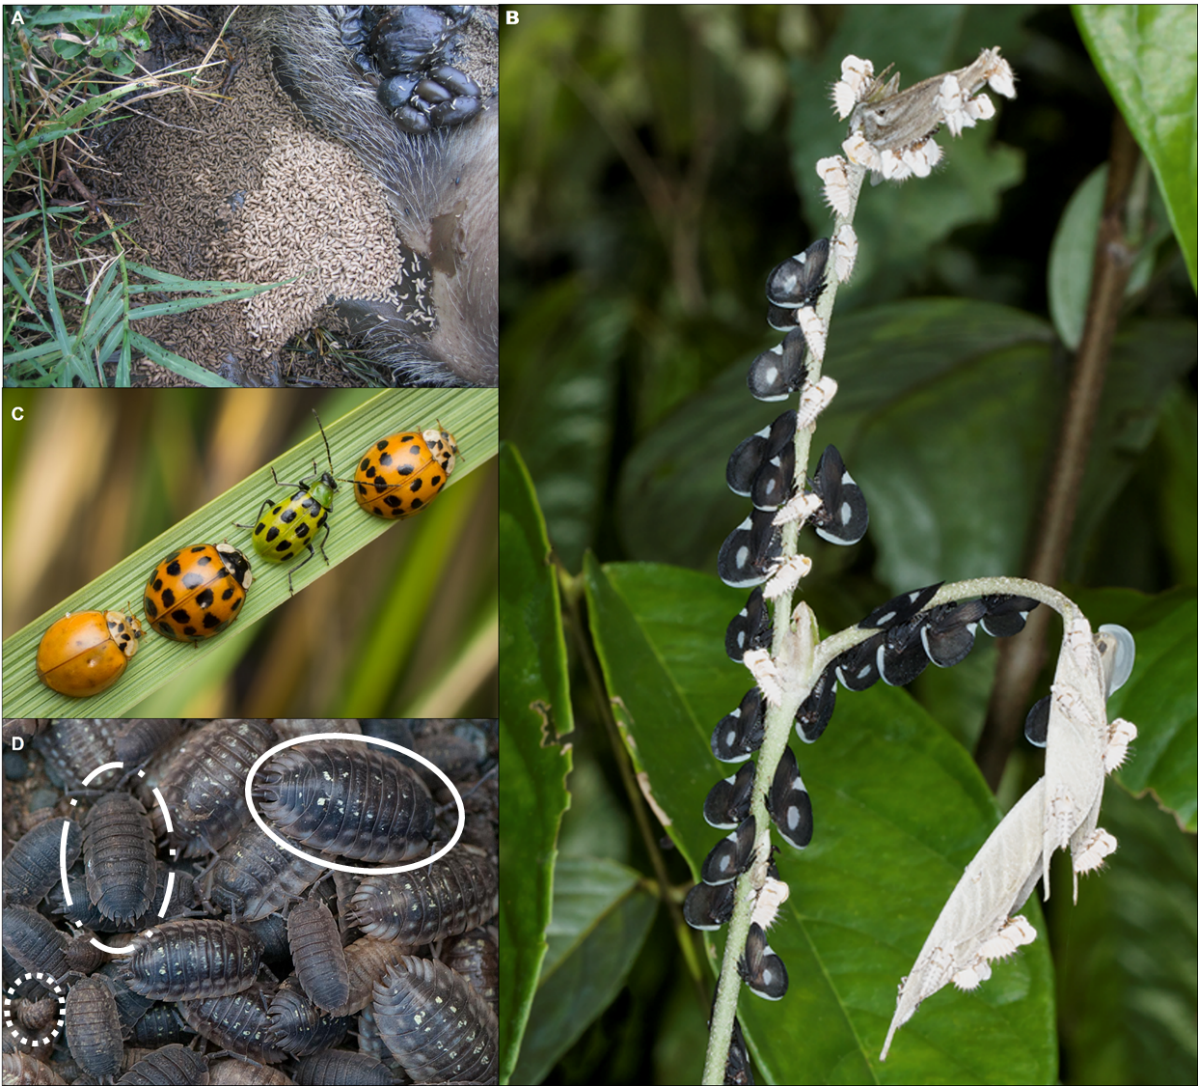
\includegraphics[width=0.9 \textwidth]{Figures/agreg_th_se.png}
		\rule{35em}{0.5pt}
	\caption[AgregMix]{\textbf{A.} Large mixed-species group of necrophagous Diptera larvae (\textit{Chrysomya albiceps} (dark maggots) and \textit{C. marginalis} (light maggots). Species segregation is observed due to the specific thermal preferences of the larvae (used with permission – Cameron Richards). \textbf{B.} Lady beetles (\textit{Harmonia axyridis}) and the spotted cucumber beetle (\textit{Diabrotica undecimpunctata}) on grass (used with permission - Nash Turley). \textbf{C.} Large mixed-species group of woodlice composed of three species (\textit{Armadillidium vulgare} (dotted circle), \textit{Oniscus asellus} (plain circle) and \textit{Porcelio scaber} (dashed and dotted circle); creative commons - Dave Ingram). \textbf{D.} A mixed-species group of treehoppers composed of adults and nymphs (white) of \textit{Membracis elevata} (black adults with a white spot on their back) and \textit{M. dorsata} (adults without a white spot) found in Ecuador (use with permission - Robert Oelman).}
	\label{fig:agregmix}

\end{figure}
    
%----------------------------------------------------------------------------------------
%	SECTION 4
%----------------------------------------------------------------------------------------
	\section{Benefits}
Aggregation is one of the mechanisms that can explain the coexistence of multiple species in patchy environments \cite{ives_aggregation_1991}. The advantages of mixed-species groups can be attributed to the increase in group size, which also occurs in non-mixed groups, and individuals cooperate to reach an optimal group size so that each individual will gain direct benefits. However, while it may seem that the benefits of grouping are more or less equally shared when individuals belong to the same species, this assumption becomes questionable for groups composed of different species. Surprisingly, even though mixed-species groups are interesting models to explore such questions, almost no experimental data can be found in the literature. Some examples of the benefits offered by mixed-species groups include protection against predators, protection against environmental constraints and foraging advantages resulting from aggregation behavior \citep{parrish_complexity_1999,riipi_multiple_2001,weed_benefits_2010}. 

		\subsection{Protection against predators}
One of the best studied benefits of aggregation is protection against predators, and this behavior is commonly believed to be one of the main advantages of aggregating in non-mixed and mixed-species groups \citep{evans_insect_1990,vulinec_collective_1990}. 
Cooperative defense, or the many eyes and ears theory, is one of the few benefits that have been studied in mixed-species groups. This advantage can be provided more efficiently in a mixed-species group than in a conspecific one because individuals of each species use their specific attributes to detect predators. For example, \textit{Panulirus guttatus} (a reef-obligate lobster) and \textit{P. argus} (a temporary reef-dwelling lobster) form mixed-species groups, and the two species are able to both perceive interspecific aggregation cues as well as each other’s alarm odors \cite{briones-fourzan_influence_2008}. These species share the same predators \cite{lozano-alvarez_coexistence_2007}, which can be better avoided by sharing alarm odors. 

		\subsection{Protection against the environment}
Aggregation by woodlice has been shown to offer protection against water loss (Figure \ref{fig:agregmix}; \cite{broly_effects_2014}). Woodlice are fully terrestrial crustaceans that are very sensitive to water loss, and \citet{hassall_effects_2005} demonstrated that two species of woodlice, \textit{Porcellio scaber} and \textit{Armadillidium vulgare}, clump together. These authors further found that at low densities, mixed-species groups promote population growth resulting in positive fitness consequences (higher growth rates and survivorship of group members; \cite{hassall_effects_2005}). Interestingly, \textit{A. vulgare} is more resistant to desiccation than \textit{P. scaber} \cite{hassall_effects_2005}, and \citet{broly_body_2015} subsequently demonstrated that body shape explains the difference in the mass-specific water loss rates between \textit{A. vulgare} and \textit{P. scaber}. Accordingly, \textit{P. scaber} aggregates more than \textit{A. vulgare} \cite{hassall_predicting_2010}, and it can be supposed that \textit{P. scaber} joins with \textit{A. vulgare} to form a larger group that is better able to withstand low relative humidity and/or high ambient temperatures. \citet{hassall_effects_2005} also hypothesized that this type of gathering offers members an additional food resource; woodlice are detritivorous and feed on each other’s feces.

		\subsection{Food assimilation}
Living together improves the assimilation of food in some mixed-species groups, and a good example is the larvae of carrion flies on a decaying cadaver (Figure \ref{fig:agregmix}; \cite{rivers_physiological_2011}). Maggot masses can contain hundreds to thousands of individuals from several species and instars, and the larvae secrete digestive enzymes (from their salivary glands) and mechanically liquefy muscles to facilitate the assimilation of food (exodigestion). This benefit is likely a consequence of a simple numerical effect; if more individuals are present in a group (regardless of the species), more salivary enzymes are produced \cite{wilson_impacts_2015}. \citet{dos_reis_larval_1999} observed a better survival rate in double-species groups composed of \textit{Chrysomya putoria} and \textit{Cochliomyia macellaria} when they increased the larval density of both species. They also showed that \textit{C. macellaria} is an inferior competitor in the presence of \textit{Ch. putoria}, so coexistence can occur. Obviously, such coexistence depends on the condition that the cadaver size is not limiting (competition phenomenon). \citet{ives_aggregation_1991} quantified the strength of larval competition in carrion flies and demonstrated a reduction in interspecific competition compared to intraspecific competition through resource partitioning.


%----------------------------------------------------------------------------------------
%	LE TABLEAU - DEBUT
%----------------------------------------------------------------------------------------
\begin{landscape}
\begin{table}
	\caption{Known examples of mixed-species groups in different arthropods’ taxons.\\ A: Artificial; F: Frequent; P: Punctual; R: Rare; $\uparrow$: increase; $\downarrow$: decrease; ???: unknown.}
	\label{tab:mixedsp}
	\centering
	\begin{tabular*}{\linewidth}{@{\extracolsep{\fill}}ccccccc}
		 \toprule
         \textbf{Taxons}				& \textbf{Species}		& \textbf{Life Stage}		& \textbf{Apparition}		& \textbf{Benefits}		&\textbf{Underlying}		&\textbf{References}\\
									&		&		&		&		& \textbf{Mechanisms}		&\\
		 \midrule
		\textbf{Ants}	& \textit{Manica rubida},		& Adults \& Juveniles		& A		&???		&???		&\citep{fielde_artificial_1903,errard_development_1994,vienne_congruency_1995}\\
        					& \textit{Formica selysi}	&	&	&	&	&\\	
            &	&	&	&	&	&\\                
        	& \textit{Azteca constructor},	& Adults \& Juveniles	&P	& $\uparrow$ Production of workers,	& Pleometrotic	&\citep{choe_evolution_1997,aron_les_2009}\\ 
            & \textit{A. xanthacrona}	&	&	&Better reproduction success	& (two queens)	&\\
            &	&	&	&	&	&\\
        
		\textbf{Aphids}	& \textit{Callipterinella calliptera},		& Adults \& Juveniles		& F		& $\uparrow$ Productivity of honeydew,	&Aggregation 	& \cite{hajek_coexistence_1986} \\
        & \textit{Betulaphis brevipilosa},	&	&	&Protection from predators	&pheromone?	& \\
        &	&	&	&	&	&\\

		\textbf{Butterflies}	& \textit{Malacosoma disstria},		& Adults \& Juveniles		&F		&Chemical protection,	&Trail-following 	&\citep{fitzgerald_specificity_1979,bogner_interspecific_1996}\\
        &\textit{M. americanum},	&	&	& Cannibalistic behavior	&abilities	&\\
        &\textit{Utetheisa sp}	&	&	&avoidance, Fitness (male	&	&\\
        &	&	&	&pheromone production)	&	&\\
        &	&	&	&	&	&\\
        
        \textbf{Carrion flies}	& \textit{Calliphoridae spp.},	&Adults \& Juveniles	&F	&Protection from 	&Shared  	&\citep{ives_aggregation_1991,dos_reis_larval_1999,woodcock_aggregation_2002,gunn_ability_2011,boulay_evidence_2013}\\
        &\textit{Sarcophagidae spp.},	&	&	&predators, Sharing 	&oviposition sites,	&\\
        &\textit{Muscidae spp.}	&	&	&salivary enzymes,	&Larval signal, 	&\\
        &	&	&	&Heat generation, &Thigmotactism,	&\\
        &	&	&	&$\uparrow$ Survival rate 	&Heat	&\\
        &	&	&	&	&	&\\
        
         \textbf{Cockroaches} &\textit{Nauphoeta cinera}, 	&Adults	&R	&???	&Chemical cues	&\cite{everaerts_changes_1997}\\
         &\textit{Leucophae maderae}	&	&	&	&	&\\
         &	&	&	&	&	&\\
         
         \textbf{Crabs} &\textit{Pagurus}	&Adults \& Juveniles	&???	&???	&???	&\cite{meadows_analysis_1973}\\
          & \textit{bernhardus},	&	&	&	&	&\\
          &\textit{P. prideauxi}	&	&	&	&	&\\
          &	&	&	&	&	&\\
          
		\end{tabular*}
\end{table}

\end{landscape}

\begin{landscape}
\begin{table}
	
	\label{tab:mixedsp2}
	\centering
	\begin{tabular*}{\linewidth}{@{\extracolsep{\fill}}ccccccc}
          \textbf{Crustaceans}	&\textit{Calappa calappa},	&Juveniles	&???	&Habitat selection	&Chemical cues,	&\cite{lecchini_ecological_2010}\\
          &\textit{Pachygrapsus}	&	&	&	&Visual cues	&\\
          &\textit{planifrons},	&	&	&	&	&\\
          &\textit{Lysiosquillina}	&	&	&	&	&\\
          &\textit{maculata},	&	&	&	&	&\\
          &\textit{L. sulcata},	&	&	&	&	&\\ 	
          &\textit{Raoulserenea sp.},	&	&	&	&	&\\ 
          &\textit{Stenopus hispidus},	&	&	&	&	&\\ 
          &\textit{Panulirus}	&	&	&	&	&\\ 
          &\textit{penicillatus}	&	&	&	&	&\\ 
          &	&	&	&	&	&\\
          &\textit{Panulirus guttatus},	&Adults	&R	&Recognition	&Chemical cues	&\citep{lozano-alvarez_coexistence_2007,lozano-alvarez_den_2001,briones-fourzan_influence_2008}\\ 
          &\textit{P. argus}	&	&	&alarm ordors,	&	&\\
          &	&	&	&Sharing shelter	&	&\\
          &	&	&	&	&	&\\
          
          \textbf{Fleas}	&40 species	&Adults \& Juveniles	&P	&Suppression of	&Reduction of the	&\citep{krasnov_aggregation_2006,krasnov_larval_2005}\\ 
          & listed by 	&	&	&host immune	&resource site	&\\
          &\citet{stanko_mammal_2002}	&	&	&	&	&\\
          &	&	&	&	&	&\\
          
          \textbf{Fruit flies}	&\textit{Drosophila sp.}	&Adults \& Juveniles	&F	&Limit fungal	&Chemical cues	&\citep{jaenike_aggregation_1991,wertheim_effects_2006,wertheim_evolutionary_2005}\\
          &	&	&	&	&Eggs-batches,	&\\
          &	&	&	&	&Non-random	&\\
          &	&	&	&	&distribution of	&\\
          &	&	&	&	&oviposition sites	&\\
          &	&	&	&	&	&\\
           
	\end{tabular*}
    \end{table}
		
\end{landscape}

\begin{landscape}
\begin{table}
	
	\label{tab:mixedsp3}
	\centering
	\begin{tabular*}{\linewidth}{@{\extracolsep{\fill}}ccccccc}
          \textbf{Lady beetles}	&\textit{Hippodamia}	&Adults	&P	& $\downarrow$ Mortality during	&Presence of	&\citep{simpson_aggregations_1975,lee_aggregation_1980,copp_temperature-dependent_1983,honek_aggregation_2007}\\ 
          &\textit{convergens, H.}	&	&	&winter, Protection 	&aphid prey,	&\\
          &\textit{tredecimpunctat},	&	&	&from predators	&Environmental	&\\
          &\textit{Hypera postica}	&	&	&and/or parasitoids?	&stimuli (T$\up{o}$, wind),	&\\
          &	&	&	&	&Chemical cues	&\\
          &	&	&	&	&	&\\
          
          \textbf{Locusts}	&\textit{Locusta migratoria}	&Juveniles	&F	&Protection from	&Chemical cues	&\citep{uvarov_grasshoppers_1977,niassy_intra-_1999}\\
          &\textit{migratorioides},	&	&	&predators	&	&\\
          &\textit{Schistocerca}	&	&	&	&	&\\
          &\textit{gregaria}	&	&	&	&	&\\
          &	&	&	&	&	&\\
          
          \textbf{Mites}	&\textit{Eotetranychus sp.},	&Juveniles	&F	&$\uparrow$ Fertility, 	&Deposition of	&\citep{slone_spatial_1999,le_goff_benefits_2011}\\
          &\textit{Tetranychus urticae}	&	&	&$\uparrow$ Silk production,	&faeces, Intraguild	&\\
          &	&	&	&$\uparrow$ Survival rate	&predation, Chemical	&\\
          &	&	&	&	&cues, Silk attraction	&\\
          &	&	&	&	&(sericophily)	&\\
          &	&	&	&	&	&\\
          
          \textbf{Scorpions}	&\textit{Buthotus judaicus},	&Adults	&P	&???	&Depends on season,	&\cite{warburg_intra-_2000}\\
          &\textit{Compsobuthus}	&	&	&	&Specialization of	&\\ 
          &\textit{werneri judaicus},	&	&	&	&scorpions for	&\\
          &\textit{Leiurus}	&	&	&	&different prey,	&\\
          &\textit{quinquestriatus}	&	&	&	&Low aggresiveness	&\\
          &	&	&	&	&	&\\
          
          \textbf{Spiders}	&\textit{Hypochilus thorelli},	&Adults \& Juveniles	&F	&Web-building,	&Chemical cues,	&\cite{hodge_conspecific_1997}\\
          &\textit{Achaearanea}	&	&	&Web-site selection	&Vibrational cues	&\\
          &\textit{tepidariorum}	&	&	&	&Silk attraction	&\\
          &	&	&	&	&(sericophily)	&\\
          &	&	&	&	&	&\\
       
    \end{tabular*}
    \end{table}
		
\end{landscape} 
          
\begin{landscape}
\begin{table}
	
	\label{tab:mixedsp4}
	\centering
	\begin{tabular*}{\linewidth}{@{\extracolsep{\fill}}ccccccc}          
     	\textbf{Stink bugs}	&\textit{Nezara viridula},	&Juveniles	&F	&Protection against	&Tactile cues,	&\citep{ishiwatari_studies_1976,fucarino_chemical_2004}\\ 
        &\textit{Chlorochroa ligata},	&	&	&dessication,	&Chemical cues	&\\
        &\textit{C. sayi, Thyanta}	&	&	&Developmental	&	&\\
        &\textit{pallidovirens},	&	&	&acceleration,	&	&\\
        &\textit{Euschistus}	&	&	&$\downarrow$ Mortality,	&	&\\
        &\textit{conspersus},	&	&	&$\downarrow$ Predation rates,	&	&\\
        &\textit{Eurydema sp.}	&	&	&Better adherence to	&	&\\
        &	&	&	&substrate	&	&\\
        &	&	&	&	&	&\\
     
     	\textbf{Termites}	&\textit{Reticulitermes}	&Adults \& Juveniles	&A	&???	&Chemical cues	&\cite{vauchot_regulation_1996}\\
        &\textit{santonensis},	&	&	&	&	&\\
        &\textit{R. lucifugus grassei}	&	&	&	&	&\\
        &	&	&	&	&	&\\
        
        \textbf{Thumbtack}	&\textit{Macrolophus}	&Adults	&P	&???	&???	&\cite{moreno-ripoll_conspecific_2012}\\
        &\textit{pygmaeus},	&	&	&	&	&\\
        &\textit{Nesidiocoris tenuis}	&	&	&	&	&\\
        &	&	&	&	&	&\\
        
        \textbf{Ticks}	&\textit{Haemaphysalis}	&Juveniles	&F	&$\downarrow$ Water loss	&Chemical cues	&\citep{sonenshine_pheromones_1985,tsunoda_interspecific_2007}\\
        &\textit{longicornis, H.}	&	&	&	&	&\\
        &\textit{megaspinosa}	&	&	&	&	&\\
        &	&	&	&	&	&\\
        
        \textbf{Treehoppers}	&\textit{Aconophora nitida},	&Juveniles	&F	&Protection from	&Stochastic phenomenon or	&\citep{olmstead_effect_1990,wood_diversity_1993}\\
        &\textit{A. mexicana}	&	&	&predators,	&Shared oviposition	&\\
        &	&	&	&Maternal care	&sites by females	&\\
        &	&	&	&	&	&\\
        
        \textbf{Trilobites}	&\textit{Ampyx, Asaphellus}	&Adults	&???	&???	&???	&\cite{rabano_linear_????}\\
        &	&	&	&	&	&\\      
             
    \end{tabular*}
    \end{table}
		
\end{landscape}     

\begin{landscape}
\begin{table}[t]
	
	\label{tab:mixedsp5}
	\centering
	\begin{tabular*}{\linewidth}{@{\extracolsep{\fill}}ccccccc}   
		\textbf{Whirligig beetles}	&\textit{Gyrinidae sp.}	&Adults	&F	&Predator avoidance,	&Mechanical stimuli	&\citep{heinrich_aggregation_1980,vulinec_aggregation_1989}\\
        &	&	&	&$\uparrow$ Defensive secretion	&(water waves),	&\\
        &	&	&	&	&Chemical cues	&\\
        &	&	&	&	&(pygidial secretion?),	&\\
        &	&	&	&	&Visual cues,	&\\
        &	&	&	&	&Orientation to	&\\
        &	&	&	&	&neighbours	&\\
        &	&	&	&	&	&\\
        
        \textbf{Woodlice}	&\textit{Porcelio scaber},	&Adults	&F	&Protection from	&Tactile cues,	&\cite{hassall_effects_2005}\\
        &\textit{Armadillidium vulgare},	&	&	&dessication,	&Chemical cues	&\\
        &\textit{Oniscus asellus}	&	&	&$\uparrow$ Production of faeces	&	&\\
        &	&	&	&(secondary food source)	&	&\\
        &	&	&	&	&	&\\
		\bottomrule
    \end{tabular*}
    \end{table}
		
\end{landscape}
 \clearpage
%----------------------------------------------------------------------------------------
%	LE TABLEAU - FIN
%----------------------------------------------------------------------------------------

%----------------------------------------------------------------------------------------
%	SECTION 5
%----------------------------------------------------------------------------------------
	\section{Species competition}
The close proximity of competitors that occupy the same ecological niche decreases food availability or the accessibility of reproductive partners, so competition can emerge between members of mixed-species groups in habitats with insufficient food resources. Indeed, even if aggregation offers advantages, there may also be unbalanced relationships or even social parasitism in mixed-species groups, which will engage the competitive abilities of each species. Moreover, mechanical exclusion of one species by another may also be observed. At first, individuals of one species cooperate with those of another to form a group, but once the group is formed and stable, species can mutually separate if their optimal group size is reached. If the two species have sufficiently different ecological niches, they can segregate but remain in contact (Figure \ref{fig:agregmix}; \cite{villet_contemporary_2010}), and it would be interesting to follow the dynamic of an aggregation at the moment when a group splits.

\citet{kuno_aggregation_1988} modified \textit{Volterra’s competition model} \cite{volterra_fluctuations_1926} and the generalized logistic function by incorporating \textit{Lloyd’s indices} of intra- and interspecific mean crowding \cite{lloyd_`mean_1967}. These upgraded models explain why some allied species coexist on the same resource patch, and \citet{kuno_aggregation_1988}) showed that \textit{(1) any increase in the patchiness of distribution facilitates intraspecific competition resulting in marked lowering of the equilibrium density for individual populations; but (2) its effect on the interspecific competition is just the opposite, relaxing the interaction and enabling different species sharing the same niche, which would otherwise be incompatible, to coexist stably.} Such models have been used to study competition exclusion in many species, but to our knowledge, these species did not form mixed groups.

In social foraging groups, \textit{the producer-scrounger game} is one of mathematical models used to describe the individual foraging strategies of group members \cite{giraldeau_social_2000}. This model highlights the exploitation of a producer’s findings (e.g., resource sites) by scroungers and predicts how foraging strategies change with food patch size. It also predicts how individuals can switch between the two strategies, scrounging or producing, until they reach an evolutionary stable strategy \cite{giraldeau_food_1999}. Such models have been used for many bird species \citep{giraldeau_social_2000,sumpter_collective_2009}, but to our knowledge, only in non-mixed species groups. This model could be modified to describe the foraging strategies of mixed-species groups by adding parameters to quantify the foraging abilities of each species. Such an upgraded model would be useful for predicting the ways in which species search and compete for resources in mixed groups.


%----------------------------------------------------------------------------------------
%	SECTION 6
%----------------------------------------------------------------------------------------
	\section{Metrics}
Different authors have used specific coefficients to study and quantify mixed-species groups. For this purpose, \citet{ives_aggregation_1991} proposed the quantity $\text{C}_{\text{A,B}}$ to measure mixed-species aggregations in carrion flies. 

\begin{equation}
	\label{equation1}
		C_{A,B}= \frac{Cov_{A,B}}{N_{A}N_{B}}  
\end{equation}

where $\text{Cov}_{\text{A,B}}$ is the covariance between species A and species B, and $\text{N}_{\text{A}}$ and $\text{N}_{\text{B}}$ are the number of ovipositing females on the same carcass or the number of emergent species A and B from individual breeding sites \cite{jaenike_aggregation_1991}. A value of 0.5 means a 50$\%$ increase in the expected number of heterospecific competitors in the same patch (i.e., if species A and species B are distributed independently) \cite{ives_aggregation_1991}. Using this parameter, Ives showed that aggregation behavior plays a major role in the coexistence of carrion fly species; he observed a 57$\%$ reduction in the average larval competition among pairs of species.
\citet{everaerts_changes_1997} used a \textit{cohabitation-coefficient} (CC) in their study of cockroaches (binary choice test between 2 resting sites):

\begin{equation}
	\label{equation2}
		CC= \frac{\sum n_{A}n_{B}}{10(N_{A}N_{B})}  
\end{equation}

where $\text{n}_{\text{A}}$ and $\text{n}_{\text{B}}$ are the respective numbers of species A and B under each shelter, and $\text{N}_{\text{A}}$ and $\text{N}_{\text{B}}$ are the total number of individuals of species A and B, respectively. A value of zero for CC indicates interspecific avoidance; a value of 0.33 represents a random distribution, and values higher than 0.33 indicate true interspecific aggregative behavior. An interesting feature of this relationship is that this coefficient can distinguish between avoidance of gregariousness and tolerance as the limit between these two behaviors (Figure \ref{fig:ever}). However, this method of quantifying mixed-species aggregations is restricted to experiments with two aggregation sites and is thus not useable under most field conditions.

 \begin{figure}[ht]
	\centering
		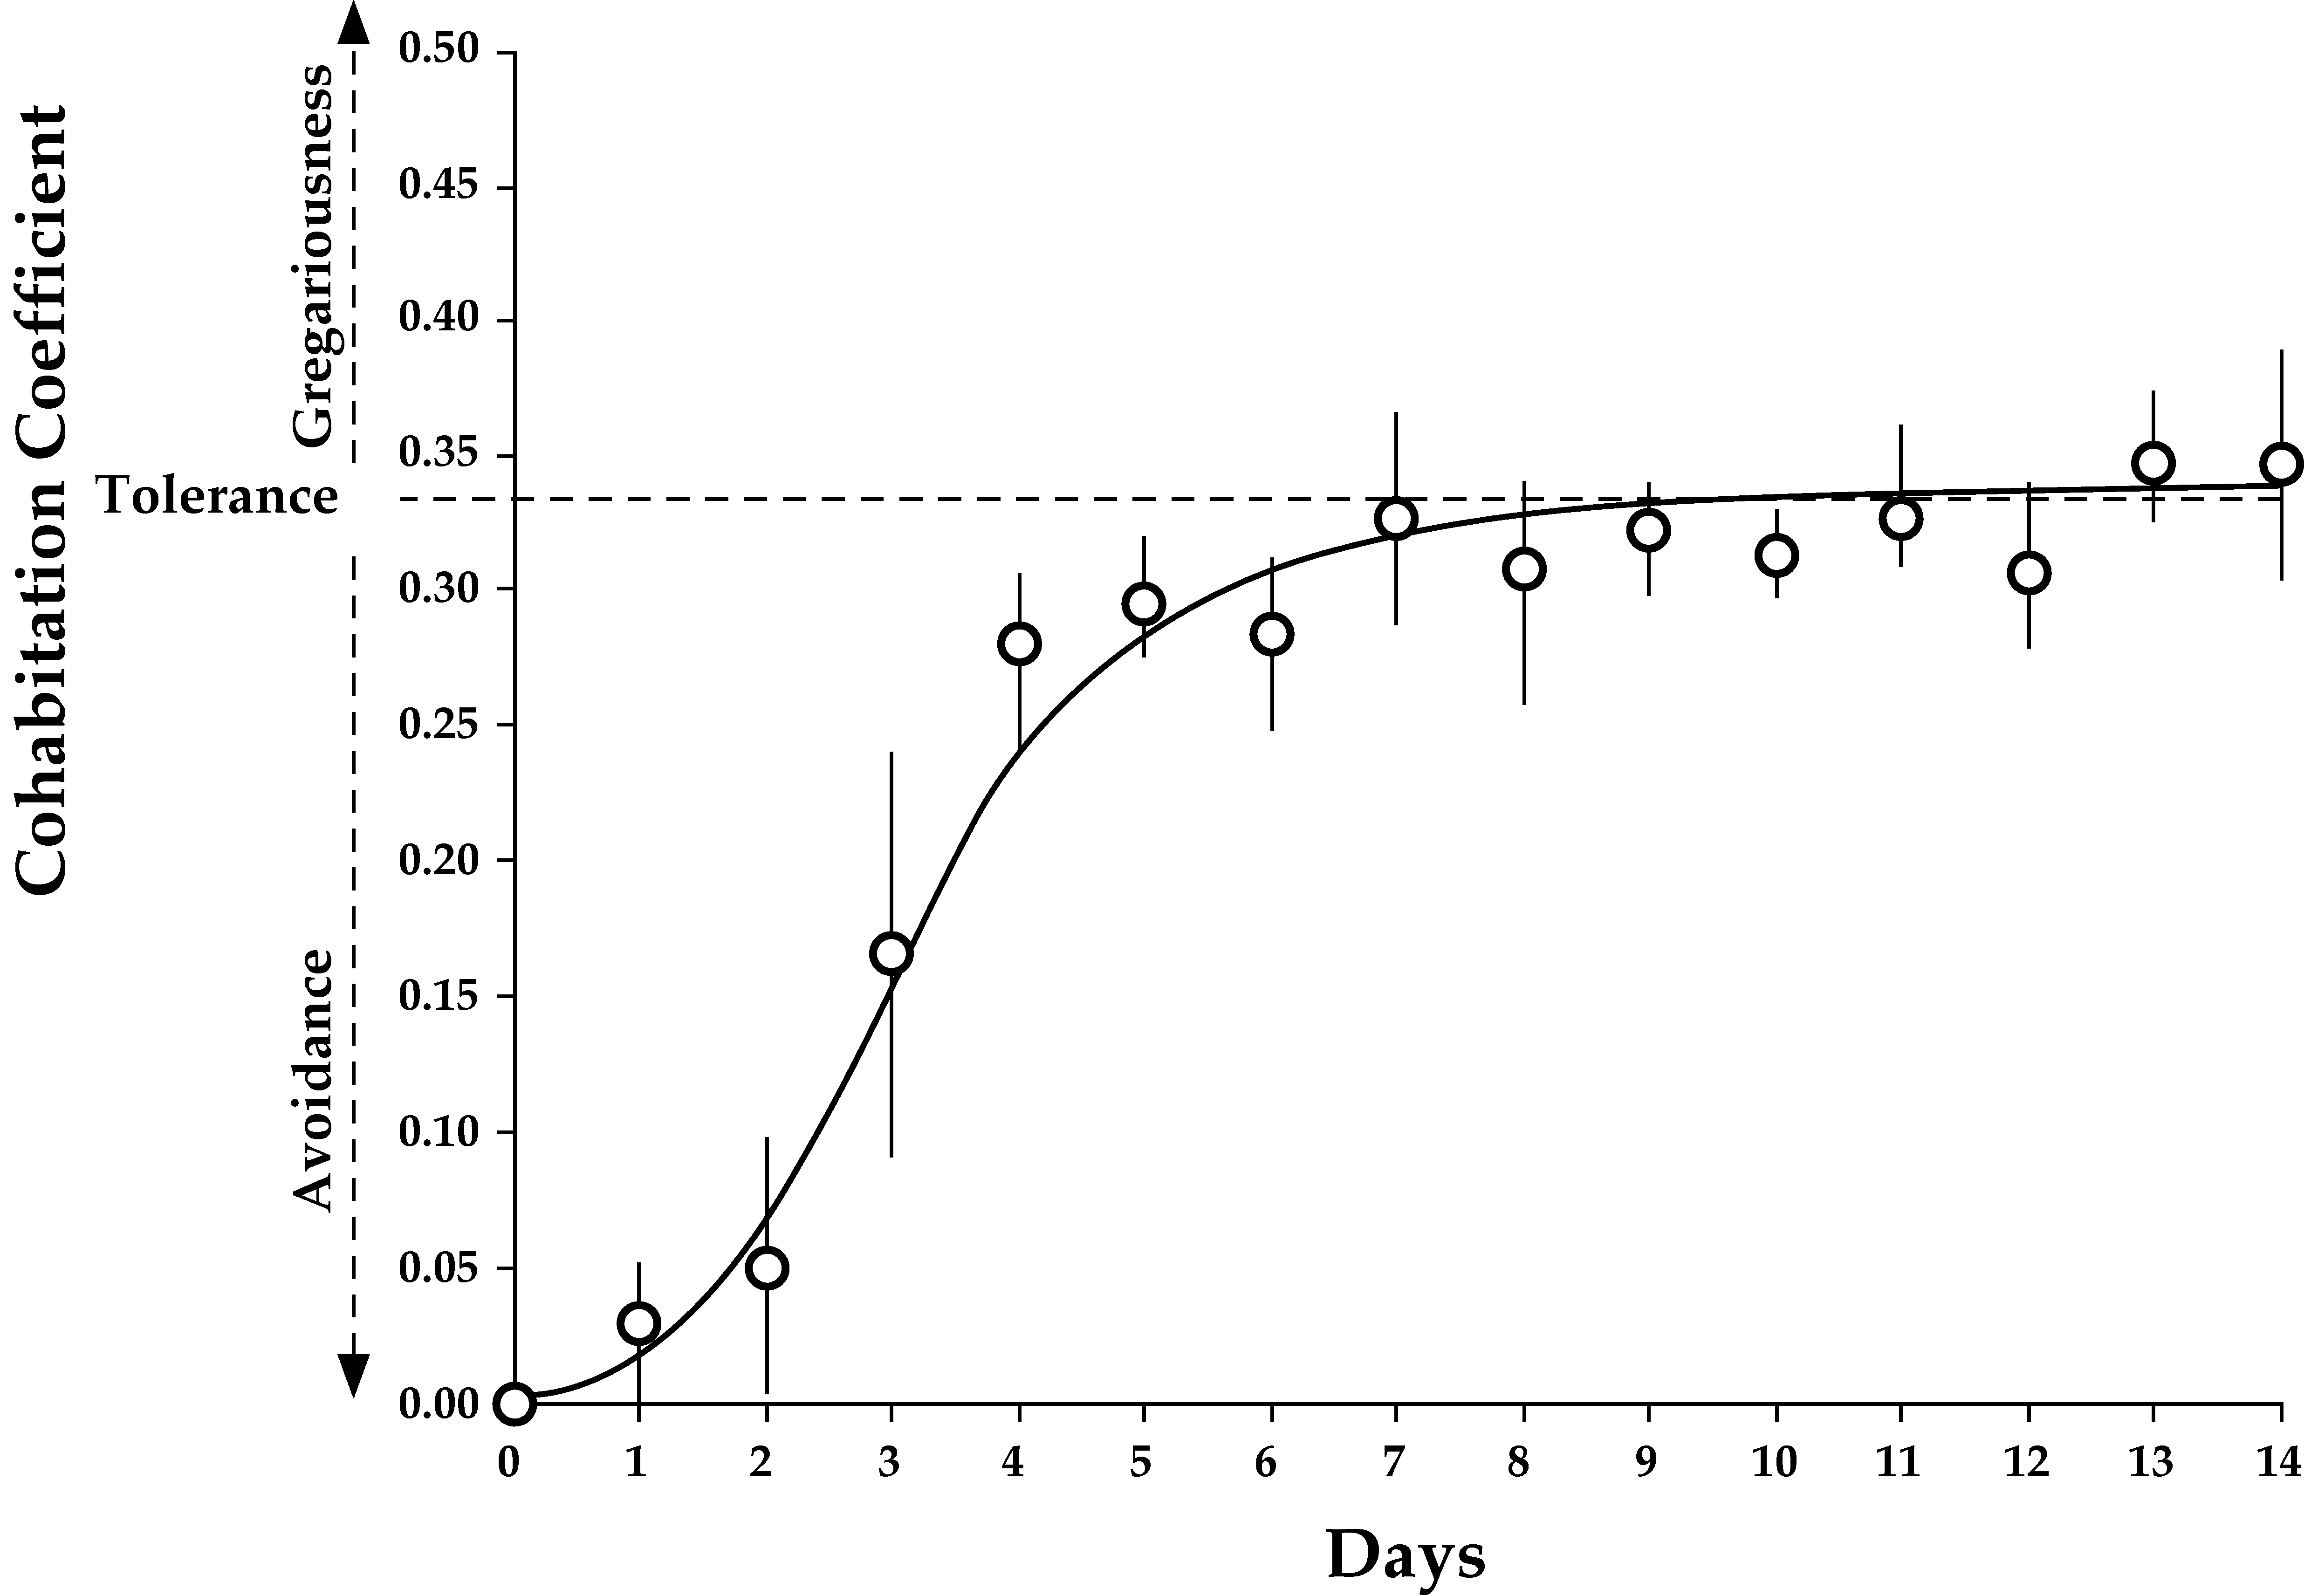
\includegraphics[width=0.9 \textwidth]{Figures/everaert_these.png}
		\rule{35em}{0.5pt}
	\caption[Ever]{The daily evolution of the \textit{cohabitation coefficient} (mean and range; equation \ref{equation2}) when two cockroach species (\textit{Nauphoeta cinerea} and \textit{Leucophaea maderae}) were maintained in heterospecific colonies (used with the permission of C. Everaerts).}
	\label{fig:ever}

\end{figure}

\citet{veech_intraspecific_2003} modified the coefficient C of \citet{ives_aggregation_1991} to measure the tendency for individuals of a species to aggregate with the individuals of other species (i.e., beetles and butterflies):

\begin{equation}
	\label{equation3}
		C= \left\lbrace\ \frac{\sum x_{i}h_{j}}{XN} - H \right\rbrace	\frac{1}{H}  
\end{equation}

where $\text{x}_{\text{j}}$ is the number of individuals at site j; X is the mean number of individuals per site; N is the number of sites; $\text{h}_{\text{j}}$ is the number of heterospecific individuals at site j; and H is the mean of all of the sites. A positive increase in C indicates an increase in the mixed-species aggregation, whereas an increasingly negative value represents interspecific repulsion. In their study, \citet{veech_intraspecific_2003} clearly showed that intraspecific aggregation decreases local species diversity, but interspecific aggregation promotes it.



%----------------------------------------------------------------------------------------
%	SECTION 6
%----------------------------------------------------------------------------------------
	\section{Examples}
Some mixed-species aggregations have been reported in arthropods, from aphids to butterflies and woodlice to ants (Figure \ref{fig:agregmix}, Table \ref{tab:mixedsp}; \cite{costa_other_2006}), and they have been observed in terrestrial, aquatic and flying arthropods (Table \ref{tab:mixedsp}). These groups can be composed of juveniles, adults or, in the majority of cases, both stages. We have listed four categories of mixed-species aggregations: frequent (F), punctual (P), rare (R) and artificial (A) (Table \ref{tab:mixedsp}). 

A frequently reported example is the mixed-species aggregation of nymph and adult treehoppers, or \textit{Aconophora species} (Figures \ref{fig:agregmix} and \ref{fig:acono}), but this aggregation involves both the mixed-species aggregation of the nymphs and a mutualism with ants. \cite{wood_diversity_1993} hypothesized that this type of mixed-species aggregation could result from transport by ants, and indeed, the ants collect sugar secreted from the nymphs and protect them from predators. Female treehoppers also aggregate their eggs in response to resource limitation (food or oviposition sites; \cite{wood_sociality_1979}), but ant attacks can occur if the nymph aggregations are disturbed by the rapid movement of adult treehoppers \cite{wood_diversity_1993}. In such cases, aggregation is supposed to allow for more efficient communication among treehopper females to prevent the attacks. Depending on the context, this mixed-species interaction can turn into either cooperation \cite{olmstead_effect_1990} or conflict \cite{wood_diversity_1993}.

 \begin{figure}[ht]
	\centering
		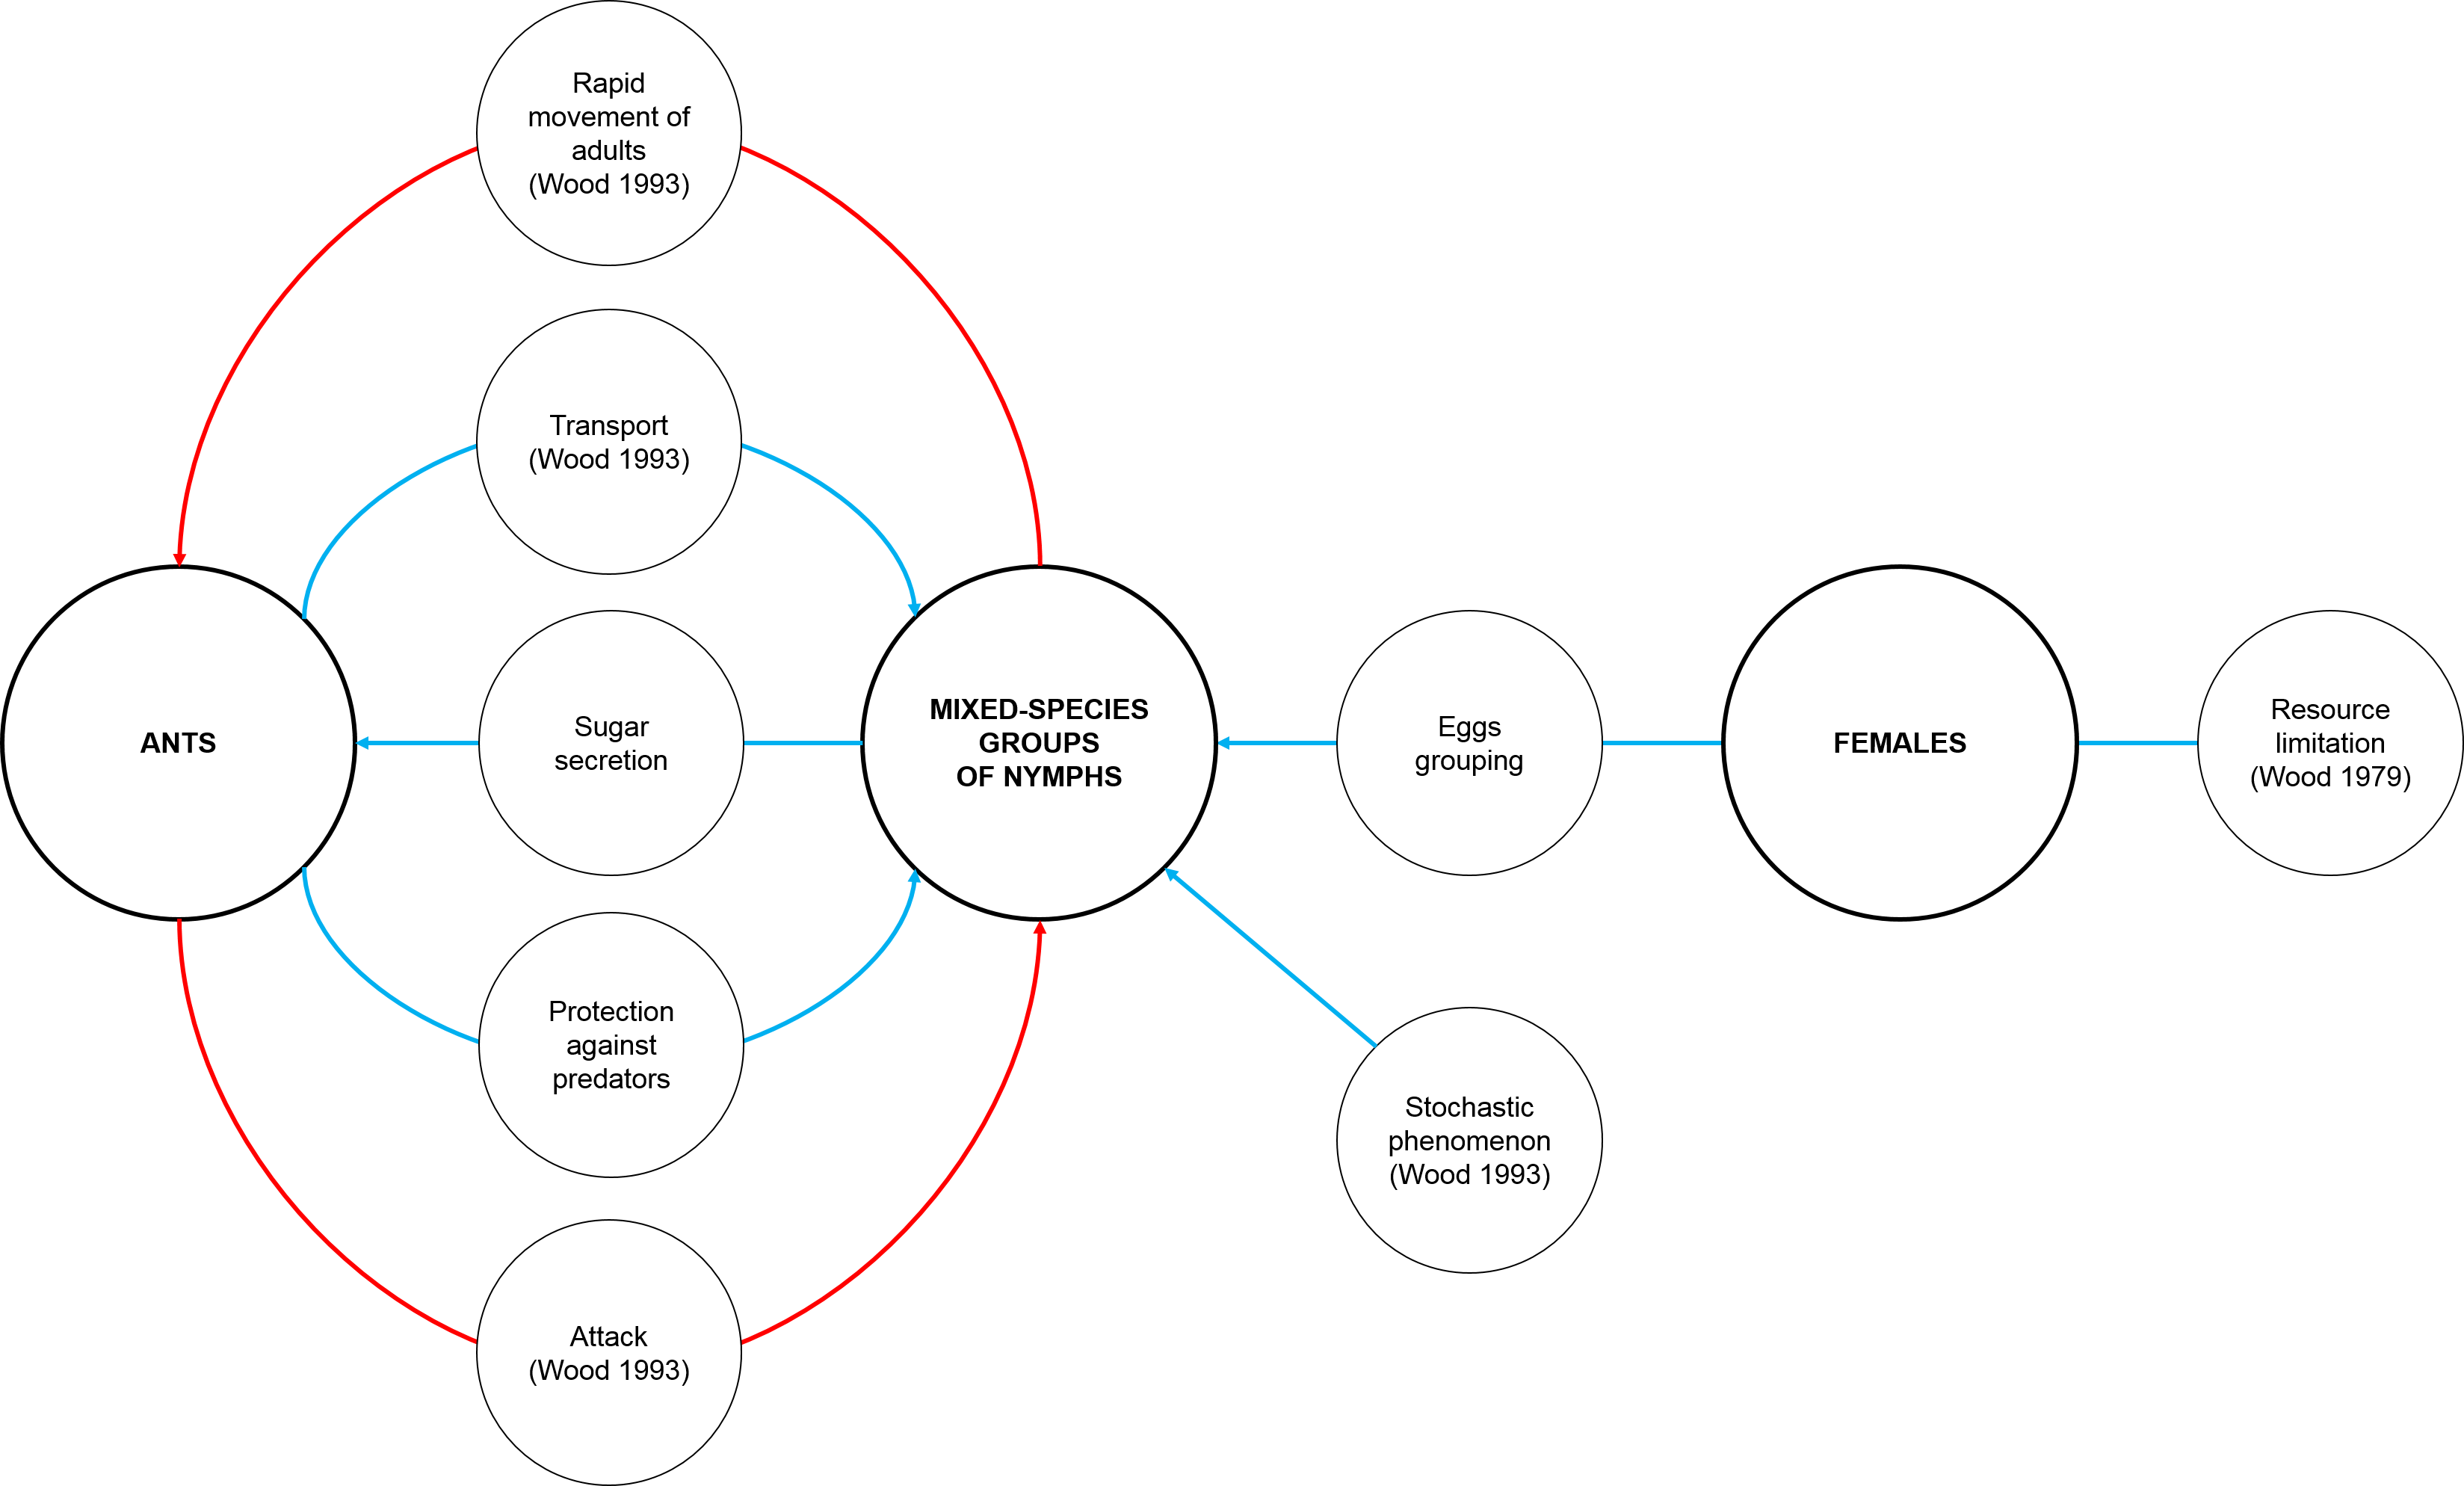
\includegraphics[width=0.9 \textwidth]{Figures/acono.png}
		\rule{35em}{0.5pt}
	\caption[Acono]{ Schematic overview of the mechanisms underlying mixed-species groups in treehoppers. Blue lines correspond to positive feedbacks that promote the formation of mixed-species groups, and red lines indicate negative feedbacks (based on Wood \citep{wood_sociality_1979,wood_diversity_1993}).}
	\label{fig:acono}

\end{figure}

Punctual mixed-species groups often appear at a given time each year. Ladybeetles, or ladybugs, form large, mixed-species aggregations inside buildings during winter \citep{simpson_aggregations_1975,lee_aggregation_1980}, and by forming such groups, ladybeetles can conserve heat and reduce their mortality due to cold \cite{copp_temperature-dependent_1983}. \citet{durieux_role_2012} highlighted the role of cuticular hydrocarbons in non-mixed Harmonia axyridis groups and identified chemical compounds, principally saturated hydrocarbons, with the capacity for heat retention on individuals \cite{durieux_role_2012}. It could be interesting to perform behavioral tests on mixed-species groups to observe the possible interspecific recognition of these hydrocarbons. Such experiments have not been performed, but they could provide interesting information about inter-specific recognition mechanisms in mixed-species groups. 

Mixed-species groups have also been observed in some lobster species, such as \textit{Panulirus guttatus} and \textit{P. argus} \citep{lozano-alvarez_coexistence_2007,briones-fourzan_influence_2008} (Table \ref{tab:mixedsp}). This type of gathering forms due to stochastic phenomena (by chance) rather the intention of individuals to aggregate \cite{briones-fourzan_influence_2008}. \textit{Panulirus guttatus} and \textit{P. argus} randomly share the same shelters \cite{lozano-alvarez_coexistence_2007}; the former tends to cling to the walls while the latter occupies the floor. \citet{briones-fourzan_influence_2008} suggested that such rarely observed mixed-species groups could be chemically mediated. Each species uses the shelter space differently, which promotes coexistence, and the aggregation allows \textit{P. argus} to share the alarm odors of \textit{P. guttatus}, enhancing protection against predators. The mechanisms underlying the avoidance behavior of \textit{P. argus} to the alarm odors of \textit{P. guttatus} remain unknown. However, \citet{briones-fourzan_influence_2008} supposed that the sedentary and defensive behavior of \textit{P. guttatus} (to go deeply into the shelter) could be sufficiently adaptive to avoid the need to recognize the alarm odors of \textit{P. argus}.

Lastly, some artificial groups have been observed but only under laboratory conditions and often in highly social species, such as ants or termites (Table \ref{tab:mixedsp}). In 1994, Errard \cite{errard_development_1994} reared \textit{Manica rubida} and \textit{Formica selysi}, two ant species, in a mixed-species colony during different time periods and observed a gradual increase in the tolerance behavior of both species over time. Furthermore, the individual hydrocarbon profiles of both species gradually acquired the chemical profile of the mixed colony \cite{errard_development_1994}. The establishment of the social group occurred in the early adult stage and was maintained through the imprint of mixed-colony cuticular hydrocarbons (imprinting-like phenomena). Interestingly, the individuals reared in the mixed-species colony were not attacked by allospecific individuals reared with non-mixed nestmates, suggesting that there is a minimal quantity of allospecific hydrocarbon compounds necessary for allospecific recognition \cite{errard_development_1994}. Such observations support the fact that mixed-species groups are composed of phylogenetically related species, which has been verified by the examples listed in Table \ref{tab:mixedsp}. Phylogenetic proximity likely facilitates cross-species recognition, a mechanisms needed to initiate and maintain mixed-species groups. Aggregates are less likely to be formed by species that relatively different phylogenetically, e.g., the ant and treehopper relationship (Figure \ref{fig:acono}; \cite{wood_sociality_1979}); the term mutualism is used to characterize such interspecific interactions. 

    
%----------------------------------------------------------------------------------------
%	SECTION 7
%----------------------------------------------------------------------------------------
	\section{Cross-species recognition}    
To create groups, animals use their ability to recognize and remain with conspecifics. Kin recognition has been well documented in several arthropod species \citep{wilson_kin_2005,costa_other_2006,jeanson_conspecific_2007,lihoreau_kin_2007,lihoreau_kin_2009,lize_kin_2010}. This recognition is mostly based on the perception of chemical cues (e.g., cuticular hydrocarbons) \citep{bell_searching_1990,chapman_insects:_1998}, and once aggregated, individuals must share information to stabilize, shape, reassemble or even split the group \cite{lachmann_advantages_2000}. This can be achieved using a range of vectors including chemical signals as well as visual recognition, and such vectors can also be used by individuals for cross-species recognition. These mechanisms imply that the aggregation vectors involved in intraspecific groups are alike, such as the similar chemical profiles of aggregation pheromones. 

		\subsection{Chemical recognition}
\citet{wertheim_evolutionary_2005} highlighted three types of interspecific interactions that are influenced by aggregation pheromones in Diptera and beetle species. The first is that aggregation pheromones are associated with microorganisms (bacteria or fungi). On plants or fruits, microbial infestation is directly associated with feeding by insects; microorganisms facilitate attack because healthy plants cannot be penetrated by larvae. For example, drosophilid females preferentially lay their eggs on host plants that have already been infested. Aggregation pheromones can also be associated with natural enemies; parasitoids that target Diptera can respond to the aggregation pheromones of their hosts \cite{wertheim_evolutionary_2005}. Lastly, aggregation pheromones can be associated with community ecology. \citet{wertheim_evolutionary_2005} described examples of cross-attraction in bark beetles. The composition of the aggregation pheromones of closely related species are similar, and this chemical similarity promotes mixed-species groups.

Another well-known example of sharing information in mixed-species groups is cockroaches. \citet{everaerts_changes_1997} reared two species of cockroaches together, namely, \textit{Nauphoeta cinera} and \textit{Leucophae maderae}, in the same environment. Far from expressing simple tolerance behavior (Figure \ref{fig:ever}), the individuals aggregated together, increasing the size of the group \cite{everaerts_changes_1997}. The authors also observed a change in the chemical profile of the hydrocarbons in both species. Under natural conditions, these chemical profiles are highly species-specific and used by cockroach species to aggregate \cite{lihoreau_kin_2009}, but when reared together, these two species established interspecific chemical communication. \citet{everaerts_changes_1997} hypothesized that this hydrocarbon transfer occurred during the frequent physical contact among group members. Such processes require relative phylogenetic proximity among species, and moreover, species likely need to be in long, cumulative physical contact to allow for chemical transfer. This contact occurs in the early life stages of individuals and persists over time. 

		\subsection{Visual recognition}
\citet{mizell_iii_congener_2012} described evidence of visual responses to conspecific and heterospecific congeners in two leafhopper species, \textit{Homalodisca vitripennis} and \textit{Oncometopia nigricans}. The authors used visual baits, such as leafhopper cadavers or colored models, to attract individuals, and the presence of conspecifics or heterospecific congeners was used to estimate the quality of the host plant. Using this information, leafhoppers chose to rejoin the heterospecific congeners or not. Similarly, \citet{lecchini_ecological_2010} showed that postlarval crustaceans preferentially used visual cues over chemical cues to detect heterospecific individuals and thus select their habitat. The presence of heterospecific crustacean congeners informs individuals about habitat quality and promotes mixed-species aggregation.


%----------------------------------------------------------------------------------------
%	SECTION 8
%----------------------------------------------------------------------------------------
	\section{Conclusion}  
Based on this review of the literature on mixed-species groups, mixed-species aggregations are found in a wide range of arthropod taxa (Table \ref{tab:mixedsp}). Such groups are not restricted by the degree of sociality of the species; they were observed in species ranging from presocial to eusocial. However, mixed-species grouping is restricted to species that live together or at least have the same habits. In other words, species that form stable social groups are more likely to accept individuals from other species, but mixed-species groups are usually composed of phylogenetically related species. This is likely due to the cross-species recognition process, which is essential for initiation and maintenance of a group. Closely related species are likely to share similar aggregation vectors (e.g., related chemical compounds), which facilitates their detection by heterospecific individuals and thus the formation of mixed-species groups. Chemical compounds are the most common aggregation cues used by arthropods in nature, and this communication can be olfactive, as in bark beetles \cite{wertheim_evolutionary_2005}, or tactile, as in cockroaches \cite{everaerts_changes_1997}. The study of cross-species detection of chemical signals is an interesting starting point to understand the mechanisms driving mixed-species aggregation, especially in the context self-organization. 

Compared to mixed-species groups, our understanding of intraspecific groups is more comprehensive (see the review by \citet{jeanson_key_2012}). Many of the experimental designs used to study monospecific groups, such as the binary choice test used by Leoncini and Rivault \cite{leoncini_could_2005}, can be applied to mixed-species groups of arthropods. Several marking techniques also exist to follow individuals, facilitating monitoring during experiments \cite{hagler_methods_2001}. Such experimental backgrounds provide a good working basis for further experimentation on mixed-species groups. Moreover, mathematical models have been developed to quantify mixed-species groups, but to our knowledge, models of the cooperation-competition phenomenon need to be established for mixed-species groups.

Mixed-species groups of arthropods provide similar benefits to members as intraspecific groups as well as those observed in mixed-species groups of mammals \cite{stensland_mixed_2003}. These benefits essentially include enhancing protection against predators and shared foraging strategies (Table \ref{tab:mixedsp}). Mixed-species groups can be stable, and the benefits can be shared among species if they do not have the same ecological niche or if resources are not limiting. However, interspecific competition can quickly turn the benefits toward one species at the expense of the other.

%----------------------------------------------------------------------------------------
%	SECTION 9
%----------------------------------------------------------------------------------------
	\section{Acknowledgments}  
Authors would like to thanks Claude \textsc{Everaerts} (Univ. Bourgogne), Robert \textsc{Oelman} (Photographer), Cameron \textsc{Richards} (PhD) and Nash \textsc{Turley} (Post-Doc) for giving us the permission of reuse their figure or photos.


\clearpage
    
    
        
    
    
    
    




% Chapter Template


\chapter{Evidence of active aggregation behaviour in \emph{Lucilia sericata} larvae and possible implication of a conspecific mark} % Main chapter title

\label{Chapter2} % Change X to a consecutive number; for referencing this chapter elsewhere, use \ref{ChapterX}

\lhead{Chapitre 2. \emph{Evidence of active aggregation behaviour of larvae and possible implication of a conspecific mark}} % Change X to a consecutive number; this is for the header on each page - perhaps a shortened title

Julien \textsc{Boulay}\up{a,b}, Cédric \textsc{Devigne}\up{a,c}, Didier \textsc{Gosset}\up{a} and Damien \textsc{Charabidzé}\up{a}

\up{a} Univ. Lille, CHU Lille, EA 7367 - UTML - Unité de Taphonomie Médico-Légale, Lille, France\\
\up{b} Université Libre de Bruxelles, Unit of Social Ecology, Brussels, Belgium\\
\up{c} UCLille, FLST, Laboratoire Ecologie et Biodiversité, Lille, France\\


Article publié dans \emph{Animal Behaviour}, 85:6, 1191-1197, 2013.

\cleardoublepage

%----------------------------------------------------------------------------------------
%	SECTION 1
%----------------------------------------------------------------------------------------
\section{Highlights}
\begin{itemize} 
\item[\tiny{$\blacksquare$}] The aggregation took place quickly and increased with time.
\item[\tiny{$\blacksquare$}] Our results suggest that thigmotaxis affects larval distribution.
\item[\tiny{$\blacksquare$}] Our results suggest that larvae deposit a mark that is detected by the other larvae.
\item[\tiny{$\blacksquare$}] Larvae are able to detect and to stay in the zone where this signal is deposited.
\item[\tiny{$\blacksquare$}] This mark is a potential vector of aggregation in this species.
\end{itemize}


%----------------------------------------------------------------------------------------
%	SECTION 2
%----------------------------------------------------------------------------------------

\section{Abstract}

Vectors of aggregation are well known for some arthropod species, but not for many others. We aimed to describe larval aggregation (experiment 1) in the carrion fly, \textit{Lucilia sericata} (Diptera: Calliphoridae), and to investigate the effect of food and conspecifics on larval behaviour (experiment 2). In experiment 1, 40 larvae were placed in a petri dish with a homogeneous diet for 30min, 1h, 3h, 5h or 24h. This experiment demonstrated for the first time under controlled conditions the active aggregation of \emph{L. sericata} larvae. The results indicate that the aggregation took place quickly and was reinforced with time. After only 3h, one main aggregate comprising a majority of individuals was observed. These results also highlight the likely use by necrophagous larvae of a signal left by conspecifics as an aggregation vector. In experiment 2, we used a video-tracking system to investigate whether such an aggregative signal exists. Fed and starved larvae were tracked for 5 min in a circular area with each half marked with a different signal combination. The time spent in the signal zones, the distance travelled, the velocity, the time at the stop and the number of stops in each zone were measured. The larvae were significantly retained by a signal (mark) left by conspecifics. Together, the results of this study demonstrate the existence of a contact and/or odour-mediated signal involved in the aggregative behaviour of necrophagous larvae.

\emph{Keywords:} binary choice - blow fly larva - gregariousness - individual distribution - larval mass - \textit{Lucilia sericata} - retentive signal - self-organization - thigmotaxis - video tracking.

\clearpage
%----------------------------------------------------------------------------------------
%	SECTION 3
%----------------------------------------------------------------------------------------

\section{Introduction}

Blow flies (Diptera: Calliphoridae) are mostly oviparous. Females lay their eggs on carcasses, and the hatched larvae feed on the decaying meat. Blow flies are usually found in large masses of hundreds to thousands of larvae \citep{ives_aggregation_1991,slone_thermoregulation_2007}. One of the most impressive consequences of these aggregations of necrophagous dipteran larvae is the elevation of temperature inside the aggregation \citep{slone_thermoregulation_2007, charabidze_larval-mass_2011}. This local increase in temperature can reach 25\up{o}C above ambient temperature and is strongly correlated with the number of larvae \citep{charabidze_larval-mass_2011}. Furthermore, temperature inside larval masses appears to be regulated by several feedback loops, such as the evaporation of humidity from the individuals towards the surface, which could accentuate the cooling phenomenon \citep{slone_thermoregulation_2007, nelson_thermal_2009, rivers_physiological_2011}. Because the development of blow fly larvae is temperature dependent \citep{huckesfeld_feel_2011}, their gregarious behaviour may be an efficient mechanism to reduce development time and thus increase larval survival. Furthermore, aggregation prevents larval desiccation, decreases the risk of predation \citep{putman_dynamics_1977} and allows insects to exploit resources better \citep{hobson_studies_1932}. Thus, aggregation behaviour appears to be fundamental for the survival of necrophagous larvae \citep{slone_thermoregulation_2007, nelson_thermal_2009}. Gregariousness in necrophagous larvae is consistent with the Allee effect theory \citep{stephens_consequences_1999}, which asserts that the presence of many congeners in a single place confers benefits on all individuals \citep{stephens_consequences_1999, etienne_interaction_2002, woodcock_aggregation_2002, allen_group_2010}.

In such cases, self-organization theory is often invoked to explain how complex collective behaviour, such as aggregation, can emerge from simple individual interactions \citep{deneubourg_collective_1989,bonabeau_self-organization_1997,bonabeau_auto-organisation_1997,camazine_self-organization_2001,sumpter_collective_2009}. In this context, the aggregation behaviour exhibits positive feedback on insect behaviour at the individual level \citep{bonabeau_auto-organisation_1997}. This positive feedback allows an amplification of the system and generates a particular structure (e.g. the aggregation). This feedback is possible only if communication exists between group members \citep{deneubourg_dynamics_2002}.

The aggregation signals used by necrophagous dipteran larvae have been little studied and are poorly understood. To our knowledge, no experimental study has yet considered the signal underlying the aggregation behaviour of necrophagous calliphorid larvae. Because larvae are aggregated upon hatching (females lay clusters of hundreds of eggs on carcasses, which possibly plays a role in the aggregation), one can ask whether a signal is used to initiate and/or stabilize the aggregation. In this context, we focused on testing two points: (1) whether carrion fly, \textit{Lucilia sericata}, larvae have an efficient gregarious behaviour under controlled conditions and (2) whether the previous presence of larvae is a retentive signal for subsequent conspecifics.


%----------------------------------------------------------------------------------------
%	SECTION 4
%----------------------------------------------------------------------------------------
\section{Material and Methods}

%-----------------------------------
%	SUBSECTION 1
%-----------------------------------

\subsection{Insect rearing}
The experiments were performed on \textit{L. sericata} larvae that were obtained from rearing colonies bred at the Forensic Institute of Lille (Nord, France). Adults were reared at ambient temperatures (25 $\pm$2\up{o}C) and natural light. Flies were fed ad libitum with caster sugar and water. Beginning with the adult fly emergence (day 0), minced beef liver was added for 7 days (day 7) to provide the proteins necessary for vitellogenesis. After 5 days with no food, liver was again provided to trigger egg laying (day 12). Eggs were placed on the breeding substrate (100g of fresh minced liver), and the temperature was set to 17 $\pm$0.5\up{o}C (day 13). Only those larvae aged between 5 and 6 days (day 18–19, corresponding to young third instars, 10 $\pm$2mm long) were used for experiments \citep{grassberger_effect_2001}. At this age, larvae have the same sensory responses as second-instar larvae \citep{cobb_what_1999}.

%-----------------------------------
%	SUBSECTION 2
%-----------------------------------

\subsection{Experiment 1: Larval Aggregation Over Time}
Forty larvae were randomly introduced into a glass petri dish (diameter = 17cm) filled to 1cm depth with a homogeneous diet. The diet was made of 20g of agar, 50g of yeast and 20$\%$ pig's blood diluted in 1 litre of water \citep{daniels_simple_1991}. The temperature of the dishes was maintained at 25\up{o}C during time t (0h, 0.5h, 1h, 3h, 5h and 24h). After time t, the dishes were instantaneously divided into 4cm\up{2} squares using a plastic lattice, creating a total of 54 quadrats. The number of larvae present in each quadrat was counted. An aggregation was defined as a peak number of individuals in a single quadrat. Because we had to destroy their environment to count the larvae that were present in each quadrat, we performed only five replicates for each observation time.

The distribution index I was calculated for each replicate r to estimate the intensity of aggregation. The index is given by Ir = $\frac{SD\up{2}}{\mu}$ where $\mu$ is the mean percentage of individuals observed among all quadrats, and SD is the standard deviation \cite{canard_quelques_2004}. In some replicates, a few larvae were lost during the counting. To homogenize the data, we used the mean percentage of individuals in the calculation of I instead of the mean number.

The radial distribution of the individuals was obtained by dividing the arena into three concentric circles with radii of r$_{1}$ = 3cm, r$_{2}$ = 6cm and r$_{3}$ = 8.5cm. The percentage of individuals present in each circle was noted and compared to a theoretical distribution. This method is described in detail in \citet{sempo_integration_2006}.

%-----------------------------------
%	SUBSECTION 3
%-----------------------------------

\subsection{Experiment 2: Effects of Signals on Behaviour}
Prior to the experiments, the larvae were removed from the breeding substrate, placed in wet pine sawdust and isolated in the dark at 25 $\pm$1\up{o}C. This isolation time starved the larvae and decreased their stress, while the sawdust removed traces of food from their cuticle. Two groups of larvae were tested: (1) larvae that had been isolated from the breeding substrate for 30min (fed larvae) and (2) larvae that had been isolated for 240min (starved larvae without food in their crop; according to data we collected by dissecting 10 crops, this amount of time is sufficient to starve the larvae; the mean surface area of crops was 3.4 $\pm$1.8mm\up{2} for fed larvae and 0.5 $\pm$0.2mm\up{2} for starved larvae; Mann–Whitney U test: U = 117.5, P $<$ 0.001). Larvae of the two tested groups (i.e. fed and starved larvae) were individually tracked for 5min in a binary choice test. Preliminary tests indicated that 5min was sufficient time for larvae to make a choice.

The experimental set-up consisted of a 2 cm tall cellulose Petri dish (diameter = 9cm) with a glass cover. This arena was lit from below by a dark light tube at a distance of 15cm (15W; $\lambda$ = 320–380nm). The wavelength was not perceivable by larvae \citep{strange_spectral_1961} and thus prevented any stress from light \citep{hinnemann_see_2010}. During the experiments, the temperature of the set-up was maintained at 25 $\pm$1\up{o}C in a thermostatic chamber. Because circadian activity does not affect larval locomotion behaviour \citep{joplin_effects_1999}, experiments were performed daily from 0900 to 1800 hours. After each trial, the arena and the glass cover were cleaned in a methanol bath for 2min at 20\up{o}C in an ultrasonic cleaner (Bioblock Scientific 86484) and washed with water.

The arena was virtually divided in half (equal zones) using the video-tracking software Ethovision 8.5XT (Noldus Information Technology, Wageningen, The Netherlands). The two zones corresponded to areas in which test signals were deposited. For each trial, a clean, wet, absorbent sheet of paper lined the bottom of the dish. The signals were deposited directly onto the absorbent paper. Larvae were then placed at the centre of the arena and followed by the video-tracking system. A digital camera (Bosch Dinion LTC0355; resolution: 752 $\times$ 582) was used to record larval displacement. The data were analysed using the video-tracking system. The time spent in the signal zones, distance travelled, velocity, time of each stop and number of stops in each zone were measured.

One control and two signals, Food and Larvae, were tested. In the Control trials, no test signals were deposited. The Food trials consisted of 100$\mu$l of a solution containing 3g of beef liver diluted in 50ml of distilled water. The test signal was deposited such that the signal spread over the entire zone (half of the arena). The Larvae trials included the marks created by five ‘signal’ larvae. Prior to depositing the test signals, signal larvae were starved and cleaned for 1h in wet sawdust to eliminate any food odours acquired in the breeding substrate. The signal larvae were then confined to one half of the petri dish and were free to crawl for 10 min. These larvae were removed before the start of the trials. Observations of the movement of the signal larvae indicated that their markings were homogeneously distributed on the entire half of the petri dish surface to which they were confined. One control and three binary choice combinations of these signals were tested: Control, Control versus Larvae (C versus L), Control versus Food (C versus F) and Larvae versus Food (L versus F).

%-----------------------------------
%	SUBSECTION 4
%-----------------------------------

\subsection{Statistical Analysis}
The Z test was used to test individual distribution during experiment 1. The random distribution hypothesis can be rejected if the absolute value of Z is greater than 1.96 \cite{canard_quelques_2004}. If the index of distribution I is less than 2.5, the distribution is regarded as homogeneous. If I $>$ 2.5, the distribution is considered aggregative.

The data were not normally distributed (Kolgomorov–Smirnov test), and the assumption of variance homogeneity was true (Bartlett's test). Following \citet{zar_biostatistical_2010}, the Wilcoxon signed-ranks test was used to compare the amount of time spent in either zone during each experimental trial. The total distance travelled, distance travelled in each zone, velocity in each zone, time of each stop and number of stops were analysed using nonparametric tests (Kruskal–Wallis, Wilcoxon and Mann–Whitney). Tests were performed using XLSTAT version 2011.1.03 (Addinsoft, New York, U.S.A.) and GraphPad InStat version 3.06 for Windows. All analyses used a significance level of $\alpha$ = 0.05, unless otherwise stated. For the Dunn's multiple paired comparison tests, the significance level $\alpha$ was adjusted using the Bonferroni method.


%----------------------------------------------------------------------------------------
%	SECTION 5
%----------------------------------------------------------------------------------------

\section{Results}

%-----------------------------------
%	SUBSECTION 1
%-----------------------------------

\subsection{Experiment 1: Larval Aggregation Over Time}
At the start of each trial, larvae were randomly distributed in the petri dish; the index mean at t = 0 was not significantly different from I$_{random}$ (I$_{random}$ = 2.5; I$_{t=0}$ = 3 $\pm$0.5, NS). All values of I were significantly higher than that for random distribution (I$_{random}$ = 2.5; Figure \ref{fig:agreg}), which indicated that individuals were aggregated. Aggregation was observed after 0.5h (I$_{t=0.5h}$ = 11.9 $\pm$2.1, Z = 25.3, P $<$ 0.001); however, the number of isolated individuals at t = 0.5h remained high (80$\%$ of the larvae; Figure \ref{fig:agreg}). Aggregations were mainly located at the periphery of the Petri dish, in contact with the wall (Figure \ref{fig:agreg}). The number of larvae in the largest aggregation increased with time. After 3h, more than 60$\%$ of the larvae were gathered in a single aggregation (I$_{t=1h}$ = 14.1 $\pm$7.7, Z = 28.5, P $<$ 0.001; I$_{t=3h}$ = 35.2 $\pm$23.2, Z = 50.9, P $<$ 0.001; Figure \ref{fig:agreg}). After 5h, a main aggregation containing more than 70$\%$ of the larvae was observed in each trial (I$_{t=5h}$ = 45.5 $\pm$18.4, Z = 59.2, P $<$ 0.001; \ref{fig:agreg}). After 24h, only a few minor aggregations remained, and they were mainly located in the quadrats neighbouring the main aggregation (I$_{t=24h}$ = 46.3 $\pm$24.9, Z = 59.9, P $<$ 0.001; Figure \ref{fig:agreg}). The mean index increased with time, which indicated that larvae were increasingly aggregated (Kruskal–Wallis test: T = 14.6, P $<$ 0.01; Dunn's test: I$_{t=0.5h}$ $\neq$ I$_{t=5h}$, I$_{t=0.5h}$ $\neq$ I$_{t=24h}$, I$_{t=1h}$ $\neq$ I$_{t=5h}$, I$_{t=1h}$ $\neq$ I$_{t=24h}$, P $<$ 0.01). The results of the radial distribution experiment indicated that the majority of the individuals at each observation time were located near the arena's edge, except after 24 h (Figure \ref{fig:rad}).

\begin{figure}[h]
	\centering
		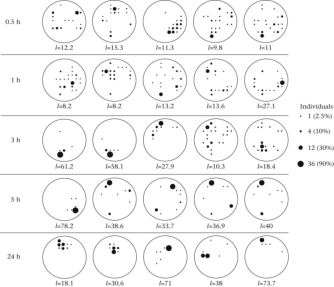
\includegraphics[width=0.9 \textwidth]{Figures/agreg_animbehav.pdf}
		\rule{35em}{0.5pt}
	\caption[Agregation]{Number of larvae aggregated in relation to time. Each large circle corresponds to one independent experiment. The sizes of black circles are proportional to the number of larvae present (40 larvae were used in each replicate). I: index of distribution corresponding to (SD)\up{2}/mean. The I for a random distribution is 2.5 and the I$_{mean}$ at t = 0 is 3 $\pm$0.5.}
	\label{fig:agreg}

\end{figure}

\clearpage

\begin{figure}[t]
\centering
		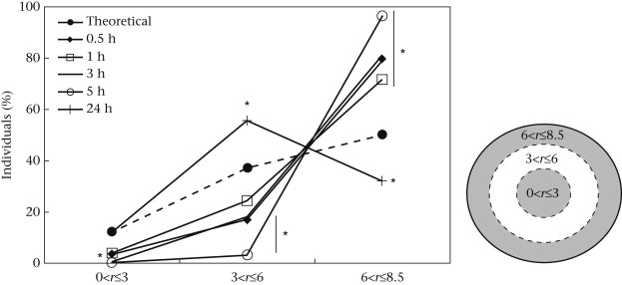
\includegraphics[width=0.8 \textwidth]{Figures/rad_animbehav.png}
		\rule{35em}{0.5pt}
		\caption[Radial]{Spatial localization of the larvae in the arena (virtually divided into three concentric circles) in relation to time (0.5, 1, 3, 5 and 24h). The theoretical distribution corresponds to a homogeneous distribution of individuals in the three concentric circles. Asterisks indicate significant differences from the theoretical distribution \\(chi-square test: N = 40 individuals).}
	\label{fig:rad}
    

\end{figure}



%-----------------------------------
%	SUBSECTION 2
%-----------------------------------

\subsection{Experiment 2: Effect of Signals on Behaviour}

\textit{Control trials}

In the Control trials, fed and starved larvae spent the same amount of time in both halves of the arena, indicating an unbiased experimental set-up (Table \ref{tab:table}, Figure \ref{fig:duree}). The distances travelled by fed and starved larvae and their velocities in each zone did not differ (Figures \ref{fig:distance} and \ref{fig:velocity}).

\textit{Control versus Signal trials}

Regardless of whether they were fed or starved, the larvae spent significantly more time in the Signal zone than in the Control zone (Table \ref{tab:table}, Figure \ref{fig:duree}). Both fed and starved larvae also traveled significantly greater distances in the Signal zone than in the Control zone (Figure \ref{fig:distance}) but moved at the same speed in each zone (Figure \ref{fig:velocity}).

In the Control versus Food trials, fed and starved larvae spent more time stationary and stopped more frequently in the Food zone than in the Control zone (Figures \ref{fig:downtime} and \ref{fig:stops}). In contrast, in the Control versus Larvae trials, fed larvae spent the same amount of time stationary and stopped the same number of times in the two zones (Figures \ref{fig:downtime} and \ref{fig:stops}). Starved larvae spent the same amount of time stationary in the two zones (Figure \ref{fig:downtime}), but they stopped more frequently in the Larvae zone than in the Control zone (Figure \ref{fig:stops}).

\clearpage


\textit{Signal versus Signal trials}

In the Larvae versus Food trials, larvae spent significantly more time in the Food zone. This result was observed regardless of whether the larvae were fed or starved (Table \ref{tab:table}, Figure \ref{fig:duree}). However, fed larvae travelled greater distances in the Food zone, whereas starved larvae travelled the same total distance in each zone (Figure \ref{fig:distance}). Unpaired comparisons of mean velocity in each zone between fed and starved larvae revealed that fed larvae moved more quickly than starved larvae in the Food zone (Figure \ref{fig:velocity}). In contrast, starved larvae spent more time and stopped more frequently in the Food zone (Figures \ref{fig:downtime} and \ref{fig:stops}).


\begin{table}[p]
	\centering
    \caption[Table]{Mean times $\pm$SD (s) spent by the fed and starved larvae in the two zones of the arena for each combination of signals}
    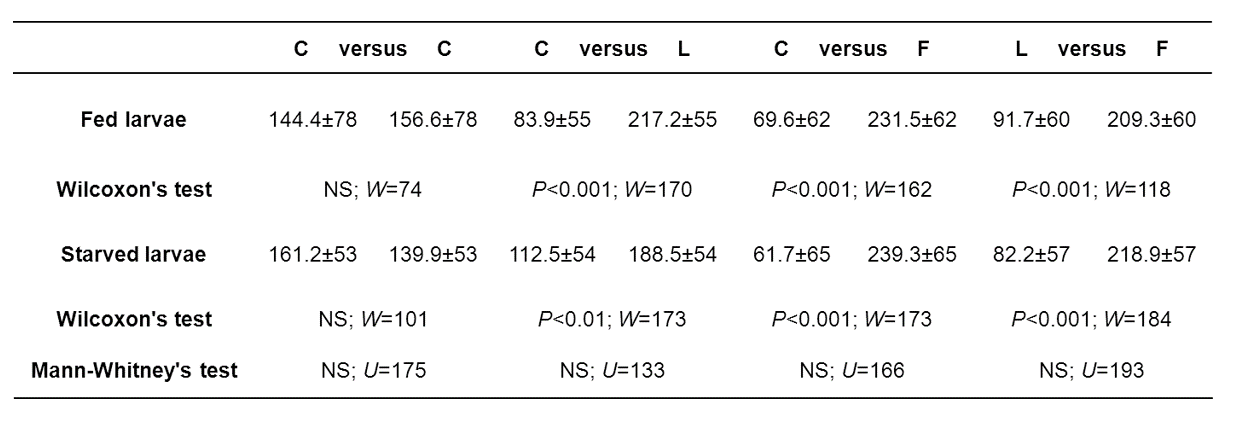
\includegraphics[width=0.9\textwidth]{Figures/table.png}
    \label{tab:table}
\end{table}

\begin{figure}[p]
	\centering
    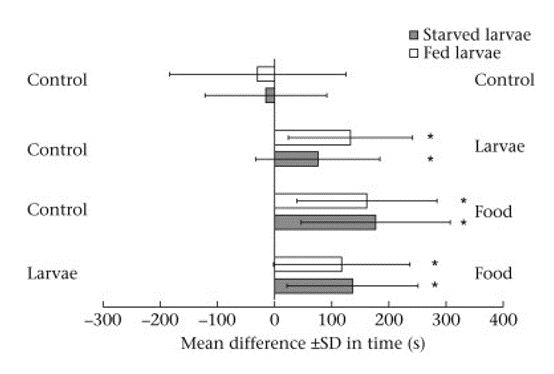
\includegraphics[width=0.9 \textwidth]{Figures/duree.png}
    \rule{35em}{0.5pt}
    \caption{Mean difference $\pm$SD in time (s) spent between signals (half zones) for fed and starved \textit{L. sericata} larvae. The mean difference was obtained by subtracting the time spent by larvae in the signal zone on the right-hand side from the time spent in the signal zone on the left-hand side. If positive, more time was spent in the former and if negative, more time was spent in the latter. Asterisks indicate significant differences between zones (Wilcoxon test: N = 20). No differences between fed and starved larvae were observed whatever the experimental condition.}
    \label{fig:duree}   

\end{figure}

\begin{figure}[p]
	\centering
    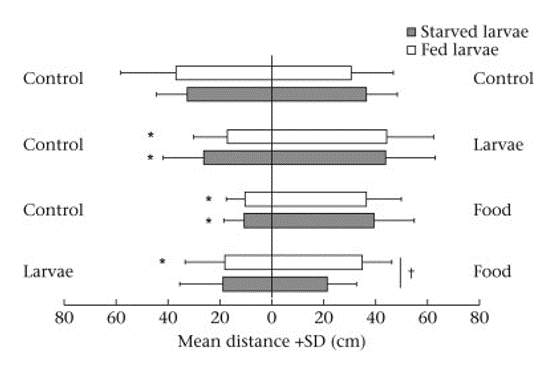
\includegraphics[width=0.8 \textwidth]{Figures/distance.png}
    \rule{35em}{0.5pt}
    \caption{Mean distances +SD (cm) travelled by fed and starved larvae in each zone of each experimental condition. Asterisks indicate significant difference between the mean distance travelled by larvae in the signal zone on the left-hand side and the mean distance travelled by larvae in the signal zone on the right-hand side (Wilcoxon test: N = 20). Dagger indicates significant difference between the mean distance travelled by fed larvae and the mean distance travelled by starved larvae in the same zone during the same condition (Mann–Whitney test: N = 20).}
    \label{fig:distance}  

	\centering
    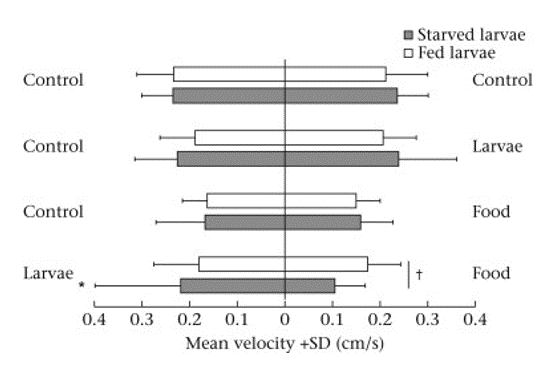
\includegraphics[width=0.8 \textwidth]{Figures/velocity.png}
    \rule{35em}{0.5pt}
    \caption{Mean velocities +SD (cm/s) recorded for fed and starved larvae in each zone of each experimental condition. Asterisks indicate significant difference between the mean velocity of larvae in the signal zone on the left-hand side and the mean velocity of larvae in the signal zone on the right-hand side (Wilcoxon test: N = 20). Dagger indicates significant difference between the mean velocity of fed larvae and the mean velocity of starved larvae in the same zone during the same condition \\(Mann–Whitney test: N = 20).}
    \label{fig:velocity}  
\end{figure}

\begin{figure}[p]
	\centering
    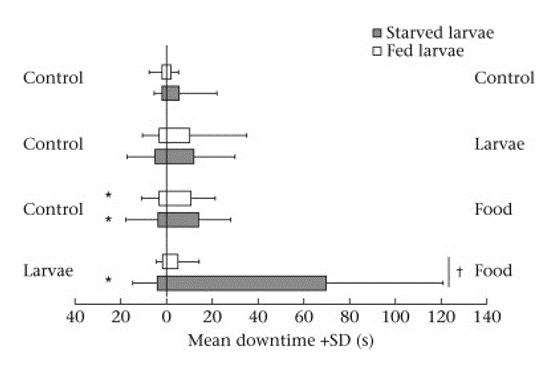
\includegraphics[width=0.85 \textwidth]{Figures/downtime.png}
    \rule{35em}{0.5pt}
    \caption{Mean time at the stop +SD (s) recorded for fed and starved larvae in each zone of each experimental condition. Asterisks indicate significant difference between the mean time at the stop of larvae in the signal zone on the left-hand side and the mean time at the stop of larvae in the signal zone on the right-hand side (Wilcoxon test: N = 20). Dagger indicates significant difference between the mean time at the stop of fed larvae and the mean time at the stop of starved larvae in the same zone during the same condition (Mann–Whitney test: N = 20).}
    \label{fig:downtime}  

	\centering
    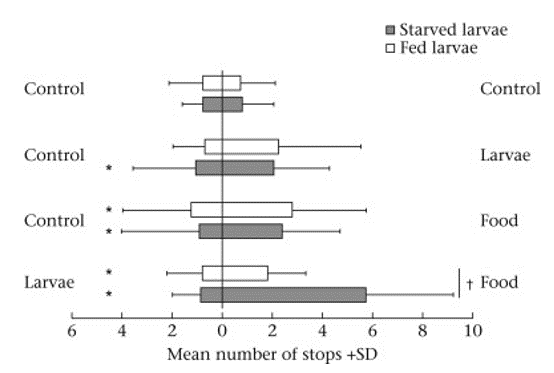
\includegraphics[width=0.85 \textwidth]{Figures/stops.png}
    \rule{35em}{0.5pt}
    \caption{Mean number of stops +SD recorded for fed and starved larvae in each zone of each experimental condition. Asterisks indicate significant difference between the mean number of stops of larvae in the signal zone on the left-hand side and the mean number of stops of larvae in the signal zone on the right-hand side (Wilcoxon test: N = 20). Dagger indicates significant difference between the mean number of stops of fed larvae and the mean number of stops of starved larvae in the same zone during the same condition (Mann–Whitney test: N = 20).}
    \label{fig:stops}  
\end{figure}

\clearpage

%----------------------------------------------------------------------------------------
%	SECTION 6
%----------------------------------------------------------------------------------------

\section{Discussion}
The gregariousness of necrophagous blow fly larvae has been extensively reported, especially in the context of forensic entomology, but rarely is the phenomenon studied under controlled conditions. In necrophagous species, aggregation behaviour is very well developed, and larvae aggregate in large masses of hundreds to thousands of congeners \citep{ives_aggregation_1991,slone_thermoregulation_2007}. This behaviour is assumed to have many benefits \citep{baxter_dynamics_1983, stephens_consequences_1999, slone_thermoregulation_2007, charabidze_larval-mass_2011, rivers_physiological_2011}, but the mechanisms of the process need to be clarified.

Our experiments showed that small aggregations appear over short timescales (0.5h) and gain more individuals over time. In other arthropod species, such as woodlice \citep{devigne_individual_2011,broly_aggregation_2012} and cockroaches \citep{jeanson_self-organized_2005}, the aggregations are formed more quickly, in approximately 5 min. Because cockroaches and woodlice move more quickly than \textit{L. sericata} larvae, the average velocity of these animals could explain the different timescales of their aggregations. The blow fly aggregations were located near the arena edge, except after 24h. These results illustrate the positive thigmotactic behaviour of blow fly larvae. Such observations have been reported in many arthropod species \citep{devigne_individual_2011, mailleux_collective_2011}. The large number of individuals present in the aggregation could explain the exception observed at 24h. After 24h, the aggregations included 30–40 larvae; the crawling effect, scramble competition and food consumption probably caused aggregations to move \citep{berrigan_how_1995}. Given this observation, the movement of the aggregation would be regulated by thigmotaxis for a small number of the larvae. In larger aggregations, the thigmotaxis between congeners is more important, as contact between congeners occurs more frequently than contact with the environment. To our knowledge, no studies have demonstrated whether such global movements are guided by a few individuals, as in human crowds \citep{dyer_consensus_2008}, primates \citep{sueur_selective_2009}  and the quorum effect \citep{sempo_complex_2009}. Furthermore, such displacement of an aggregation may simply result from mechanical phenomena (e.g. the crawling effect) and/or behavioural mechanisms (e.g. thermoregulation in the aggregation).

In mycophagous \textit{Drosophila} larvae, larval aggregation has been demonstrated to result from egg aggregation \citep{jaenike_aggregation_1991}. However, our results clearly showed that the aggregations of calliphorid larvae result from larval behaviour and are not solely attributable to the clustering of egg batches. Another common hypothesis regarding aggregation emphasizes the role of environmental heterogeneity \citep{mailleux_collective_2011, devigne_individual_2011, broly_aggregation_2012}. However, \textit{L. sericata} larvae that were randomly introduced into a homogeneous environment rapidly aggregated, and this aggregation increased with time. We conclude that the necrophagous fly larvae actively aggregate. This conclusion implies that the larvae used one or several mechanisms to gather, stabilize the aggregations and possibly move together \citep{zirbes_new_2010, mailleux_collective_2011}.

The video-tracking experiments clearly demonstrated, for the first time, the existence of a conspecific signal that can attract dipteran larvae to a given area. Our results suggest that \textit{L. sericata} larvae deposit a signal that is detected by other larvae. This signal had a movement-retentive effect and increased the amount of time that conspecifics remained in areas in which the signal was deposited. This result clearly showed not only that larvae can detect where conspecifics have been but also that they preferentially stay in those places. During the video-tracking experiments, we observed a mean velocity of 0.2 cm/s (Control trials), consistent with \citet{charabidze_modelisation_2010}. However, the presence of Food (signal) in the arena tended to decrease the mean velocity of starved larvae. Our observations indicated that starved larvae stopped and tried to eat the Food signal. This behaviour explains the decrease in the average velocity and the increase in the amount of time spent in the Food zone. The feeding behaviour is obviously related to the presence of food, but it also seems linked to the presence of other \textit{L. sericata} larvae. Indeed, in the Larvae versus Food trials, starved larvae spent more time stationary and stopped more frequently on the Food signal than the fed larvae in the Control versus Food trials. This behaviour suggests that the simultaneous presence of the two signals, although separate, influence the feeding behaviour of starved larvae. Larvae may be able to detect the larval signal from a distance, which would encourage them to feed \citep{devigne_out_2004}. Some previous studies have focused on the response of dipteran larvae to food signals \citep{christopherson_foraging_1997, cobb_what_1999, kaiser_behaviour_2008}, but no studies have addressed a possible interaction with signals deposited by conspecifics.

Lastly, both fed and starved larvae spent more time on the Food signal than on the Larvae signal (Larvae versus Food trials). Based on this result, we conclude that foraging behaviour prevails over aggregation behaviour in this species. However, the Larvae versus Food trial was a forced set-up; under natural conditions, larvae live on carcasses and thus never encounter such a choice. Furthermore, signals are deposited by larvae that have direct contact with the food source. To highlight the response of larvae to the signals deposited by congeners in an environment completely impregnated with food (seminatural conditions), experiments combining the signal larvae with the signal food are currently underway based on the same binary choice test set-up; however, these experiments combine the signal larvae with the signal food.

In addition, the young third-instar larvae used for these experiments may behave differently from one-instar or two-instar larvae. In contrast to third-instar larvae, young larvae have undeveloped mouth hooks. Because aggregation enhances the local liquefaction of tissues \citep{hobson_studies_1932}, younger larvae probably tend to aggregate to increase their access to soft food. This consideration is less important for older larvae, which can feed on solid tissues.

Our study addresses the question of aggregation mechanism at the collective level. Our experiments indicate that the aggregation of \textit{L. sericata} is an active, quick and efficient mechanism, probably mediated by larval signals. Thus, the gregarious behaviour of \textit{L. sericata} larvae probably results from dynamic processes that are mediated by attractive/retentive signals, and not only from thigmotaxis or environmental heterogeneity \citep{devigne_individual_2011, mailleux_collective_2011, broly_aggregation_2012}. Our observations at the scale of the individual also demonstrate that larvae deposit a signal that is perceived by conspecifics and has a movement-retentive effect. Together, these results strongly support the hypothesis that gregarious behaviour is mediated by a movement-retentive signal, which is deposited locally by conspecifics.

Further experiments should investigate the potential role of the larval signal on aggregation dynamics. Such data would facilitate models of larval mass over time in this and other insect species \citep{farine_gregarisme_1984, rivault_cockroach_1998, depickere_effect_2008}. Under natural conditions, larval aggregation can be interspecific \citep{amendt_current_2010} and it would be worth conducting studies of interspecific gregarious behaviour.

%----------------------------------------------------------------------------------------
%	SECTION 7
%----------------------------------------------------------------------------------------

\section{Acknowledgments}
J.B. and D.C. conceived and designed the experiments, J.B. performed the experiments, J.B. and D.C. analysed the data, J.B., D.C. and C.D. wrote the paper. Thanks to M. Daniau and E. Boulleaux for laboratory assistance and D. Toussaint for English correction. Thanks to J.-L. Deneubourg (Senior Research Associate from the F.R.S.-FNRS) for helpful suggestions and comments.


\clearpage





% Chapter Template

\chapter{A first insight in the scanning behaviour of presocial blow fly larvae} % Main chapter title

\label{Chapter3} % Change X to a consecutive number; for referencing this chapter elsewhere, use \ref{ChapterX}

\lhead{Chapitre 3. \emph{A first insight in the scanning behaviour of presocial blow fly larvae}} % Change X to a consecutive number; this is for the header on each page - perhaps a shortened title

Julien \textsc{Boulay}\up{a,b}, Cécile \textsc{Betremieux}\up{a}, Valéry \textsc{Hédouin}\up{a} and Damien \textsc{Charabidzé}\up{a}

\up{a} Univ. Lille, CHU Lille, EA 7367 - UTML - Unité de Taphonomie Médico-Légale, Lille, France\\
\up{b} Université Libre de Bruxelles, Unit of Social Ecology, Brussels, Belgium\\


Article publié dans \emph{Physiological Entomology}, DOI: 10.1111/phen.12117.\\


\cleardoublepage

%----------------------------------------------------------------------------------------
%	SECTION 1
%----------------------------------------------------------------------------------------

\section{Abstract}
Aggregation of necrophagous larvae has several benefits: the sharing of salivary enzymes (exodigestion), temperature regulation, protection from predators and parasites, etc. and is well developed in blow flies (Diptera: Calliphoridae). This study focuses on the aggregation mechanism used by the necrophagous larvae of \textit{Lucilia sericata} Meigen, the common green bottle fly. The ability of single larva to detect and follow a signal (trail) created by conspecifics is investigated initially. A circular ring is drawn in a Petri dish where twenty starved larvae have crawled for a period of 30 min. A naïve (test) larva is then placed in the dish and video-tracked. Naïve larvae are able to detect the boundaries of the larvae-crawled area and stay preferentially within this conspecific-marked zone. In a second step, the orientation of larvae by scanning, a dedicated, ground-signal detection behaviour of dipteran larvae, is analysed. Four experimental conditions are tested: control, presence of food, conspecifics, and food + conspecifics. When conspecifics have been previously present in a given area, the scanning behaviour by naïve larvae in this area decreases (both in number and frequency of scans). Accordingly, scanning by necrophagous larvae of \textit{L. sericata} should be considered not only as locomotion behaviour but also as a potential way to detect signals from conspecifics for the purpose of aggregation. The chemical composition of the attractant(s), the behavioural effects (attraction or retention) and the implication of larval signalling in the aggregation process are new fields to explore.

\emph{Keywords:} aggregation - chemo-detection - self-organization - sensory organs - trail-follwing.

\clearpage

%----------------------------------------------------------------------------------------
%	SECTION 2
%----------------------------------------------------------------------------------------
	\section{Introduction}
Aggregation, or interattraction, is a common behaviour that occurs in many biological systems \cite{krause_living_2002}. With regard to necrophagous species, the costs and benefits of aggregation by blow fly larvae have been identified and discussed by Ives (1991) and more recently by \citet{rivers_physiological_2011}. One main advantage is the capacity of large larval masses to locally modify some of the biotic and abiotic factors of their ecosystem, leading to faster larval development. The most well-known benefit of aggregation in necrophagous larvae  is the local elevation of temperature inside aggregates, called the \textit{larval-mass effect} or more familiarly \textit{maggot-mass effect} \citep{slone_thermoregulation_2007, huckesfeld_feel_2011, rivers_physiological_2011, charabidze_larval-mass_2011}. This heat generation accelerates the development of blow flies larvae, and thus decreases the time spent by larvae on carrion \citep{heaton_quantifying_2014, johnson_effect_2014}. Gregarious behaviour also offers protection from predators and parasites, cooperation for digestion, and an increase in food assimilation (reviewed by \citet{rivers_physiological_2011}). Accordingly, gregarization appears to be a key behaviour in these species, which is especially remarkable because larval masses are self-organized structures: each larva has only a local perception of its close environment and (re)acts for itself \cite{camazine_self-organization_2001}.     
Such social organization requires at least a basic communication system between individuals \cite{camazine_self-organization_2001}. In many social insect species, such as Lepidoptera or Hymenoptera, larval aggregations are mediated by tactile and/or chemical cues (see examples in \citet{wertheim_pheromone-mediated_2005} and \citet{costa_other_2006}). However, only a few studies have investigated the mechanisms underlying the collective behaviour of blow fly larvae \citep{rivers_physiological_2011, boulay_evidence_2013}. In a recent study, the present research group \cite{boulay_evidence_2013} highlighted for the first time the existence of a signal  deposited or left passively by \textit{Lucilia sericata} larvae on the substrate over which they were crawling: these chemical cues were shown to have an attractive/retentive effect on conspecifics \cite{boulay_evidence_2013}. The present study focuses on the behavioural response of \textit{L. sericata} larvae to this signal, and particularly with regard to orientation mechanisms.

\citet{green_organization_1983} describe five elementary behaviours thought to be shared by all cyclorrhaphous dipteran larvae (i.e., species where the imago emerges from the pupal case by pushing a lid or a circular seal). These are, locomotion, turning, burrowing, rearing and bending. The authors define rearing as the raising and trembling of the head and first thoracic segments, whereas bending is described as the lateral flexing of the head and anterior segments \cite{green_organization_1983}. In other words, rearing occurs in a vertical axis and does not directly affect larval trajectory, whilst bending is laterally oriented. Accordingly, \citet{green_organization_1983} assume that bending is mainly associated with changing direction (i.e., turning) during locomotion. However, observations made in this laboratory (J. Boulay and D. Charabidzé, unpublished observations) strongly suggest that larvae may also use bending to detect the chemical signals around them and to orientate accordingly. Indeed, the anterior part of the larva’s body is the location of most of the sensory organs: Calliphoridae larvae have twelve photoreceptors (Bolwig’s organ) \cite{hinnemann_see_2010}, one olfactory and one gustatory organ \citep{chu-wang_fine_1971, cobb_what_1999,chu-wang_fine_1971-1} all located in the anterior section. Bending could therefore be involved in local signal detection and should be regarded as a scanning, i.e., \textit{a mechanism by which animals move their receptors, and sometimes their bodies or appendages, so as to capture information from the environment efficiently} \cite{bell_searching_1990}. Such a behaviour has been reported for many insect species during foraging, or when searching for conspecifics, refugees or mates \cite{bell_searching_1990}. 

To test this hypothesis, the present study first analyses the ability of \textit{L. sericata} larvae to detect and follow a track previously crawled by conspecifics (Larval trail experiment). It then focuses on the scanning behaviour, which is hypothesized to be involved in the detection of the larval signal. To test the hypothesis, the scanning behaviour of \textit{L. sericata} third-instar larvae in analysed under four different experimental conditions: control, conspecific larval signal, food, and larval signal + food together \cite{boulay_evidence_2013}. According to this hypothesis, an increase of scanning behaviour should be observed in the absence of larval signal, demonstrating active searching for the conspecific’s signal (i.e. chemotaxis \cite{gomez-marin_active_2011}). 

%----------------------------------------------------------------------------------------
%	SECTION 3
%----------------------------------------------------------------------------------------
	\section{Material and Methods}
%----------------------------------------------------------------------------------------
%	SUBSECTION 1
%----------------------------------------------------------------------------------------    
        	\subsection{Insect rearing}
The experiments were performed on \textit{L. sericata} larvae that were obtained from rearing colonies (Lille, France). Adults were reared at ambient temperature (25 $\pm$ 2 \up{o}C) under natural light  and fed ad libitum with caster sugar and water. Beginning with the adult fly emergence (day 0), fresh minced beef liver was added for seven days (day 7) to provide the proteins necessary for vitellogenesis. After five days with no food, liver was provided again to trigger egg-laying (day 12). Eggs were placed on breeding substrate (100 g of fresh minced beef liver) at 17 $\pm$ 0.5 \up{o}C (day 13). Five-to-six-day-old larvae (day 18–19, corresponding to young third instars, 10 $\pm$ 2 mm long) were used for experiments \cite{grassberger_effect_2001}. During the experiments, the temperature of the set-up was maintained at 25 $\pm$ 1 \up{o}C in a thermostatic chamber.         
    
%----------------------------------------------------------------------------------------
%	SUBSECTION 2
%----------------------------------------------------------------------------------------   
			\subsection{Larval trail experiment}
This experiment was designed to test the ability of \textit{L. sericata} larvae to follow a track created by conspecifics (i.e., a trail). The setup consists of a Petri dish (diameter: 18.5 cm; surface: 268.60 cm\up{2}; Figure \ref{fig:setup}) lined with a wet paper towel (humidified with distilled water) covering the arena surface. Two smaller Petri dishes were used to circumscribe a ring (internal diameter: 5 cm, external diameter: 4.75 cm; thick: 2 cm, surface: 37.11 cm\up{2}; Figure \ref{fig:setup}). Under the ‘Control’ condition, no deposit was made in this ring. The larval trail condition was obtained with twenty starved larvae (cleaning and starving took place for 4 h in wet pine-wood dust; a time sufficient to obtain larvae with empty crops \cite{charabidze_discontinuous_2013}) crawling in the ring area for 30 min to create the Marked Zone (MZ; Figure \ref{fig:setup}). After 30 min, these twenty larvae and the two small Petri dishes were removed. A naïve (test) larva was placed in the centre of the arena (Centre Zone (CZ): 19.63 cm\up{2}; Figure \ref{fig:setup}) in the dark and video recorded using an infrared camera (Kamatec, Kam-HWI-SH-7204). The results were analysed with Ethovision 8.0 XT software (Noldus, Netherlands): trials started when the test larvae exited the Centre Zone for the first time and were stopped when individuals were outside the Marked Zone for at least 1 min or when they had reached the wall of the arena. Twenty replicates were performed for each condition. 

\begin{figure}[ht]
	\centering
		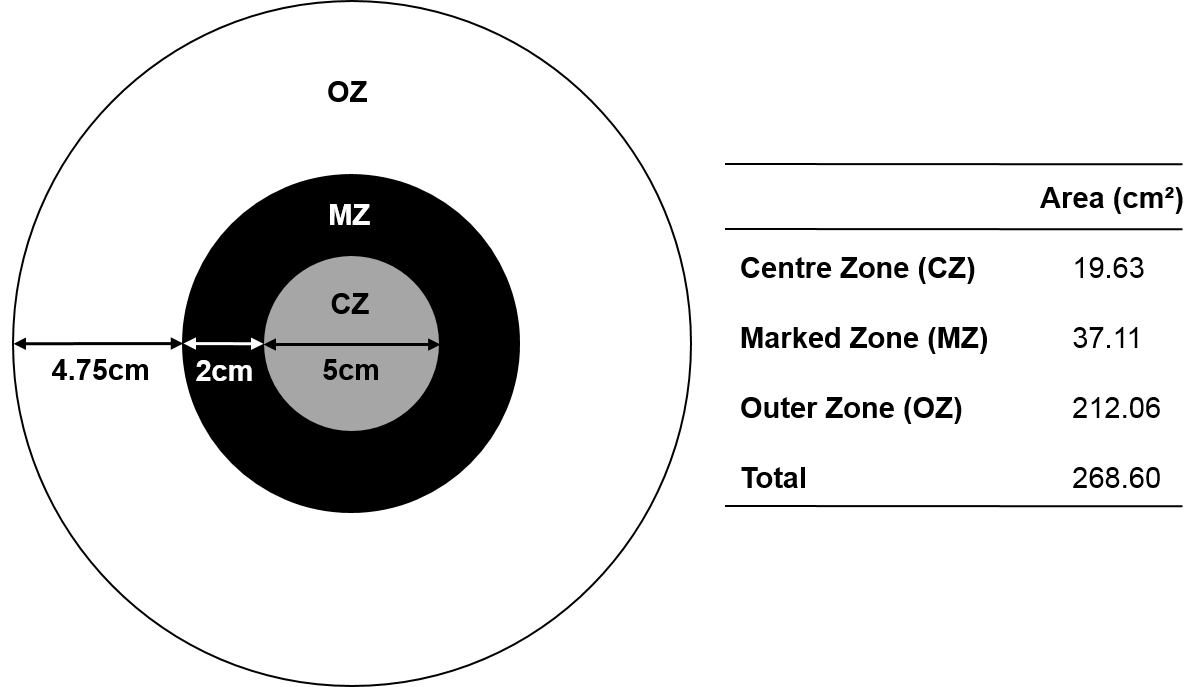
\includegraphics[width=0.9 \textwidth]{Figures/fig1.png}
		\rule{35em}{0.5pt}
	\caption[Setup]{Apparatus used for analyzing behavioural responses to the attractive signal from necrophagous larvae of the Green bottle fly, \textit{Lucilia sericata} (Control and Marked trials). Third-instar \textit{L. sericata} larvae were placed in the Centre Zone (CZ). Trials started when individuals entered in the Marked Zone (MZ) and stopped when larvae stayed more than 1 min completely in the Outer Zone (OZ).}
	\label{fig:setup}
\end{figure}

\clearpage
%----------------------------------------------------------------------------------------
%	SUBSECTION 2
%----------------------------------------------------------------------------------------   
			\subsection{Study of the scanning behaviour}
This experiment was designed to measure the scanning response according to larval signal. During scanning, the larva stopped and moved the anterior part of its body back and forth laterally (described in \citet{green_organization_1983}). The experimental set-up was a circular arena 9 cm in diameter as in \citet{boulay_evidence_2013}. Test larvae were isolated in wet pine-wood dust for 30 min prior to the experiments to remove any traces of their former breeding substrate (beef liver). A disc of clean paper towel covering the whole surface of the Petri dish was first humidified homogenously with 1.5 mL of distilled water. The ‘Control’ (C) consisted of no deposit on this paper (only the presence of distilled water). The ‘Food’ condition (F) consisted of 200$\mu$L of a solution containing 3 g of mixed beef liver diluted in 50 mL of distilled water. The solution was deposited using a micropipette such that the food solution was spread over the entire arena. The ‘Larvae’ condition (L) consisted of the signal created by ten larvae moving freely within the arena for 10 min and removed before the start of the trial. These signal-depositing larvae were previously starved and cleaned for 4 h in wet pine-wood dust (time sufficient to obtain larvae with empty crops \cite{charabidze_discontinuous_2013} to eliminate food odours acquired from the breeding substrate \cite{boulay_evidence_2013}. The ‘Larvae + Food’ condition (L + F) consisted of the deposition in the arena of both the larval signal and the food substrate (in that order). Twenty replicates were performed for each condition and individuals were followed for 5 min. Behavioural observations were video recorded using a digital camera (Bosch Dinion LTC0355) and analysed with Ethovision 8.0 XT software (Noldus, The Netherlands). Mean absolute meander/tortuosity, which is defined as the change in direction of movement of an individual relative to the distance (i.e., the amount of turning per unit distance) was used to describe the changes in larval orientation \cite{granchietti_fruit_2012} (Absolute Meander = |$\frac{Turn angle}{Distance moved}$|; \cite{noldus_ethovision:_2001}). The encoding of scanning behaviour was made from the video recording using sequenceR (a free interface developed by M. Hervé and available online (http://www.maximeherve.com/r-statistiques/sequencer)) implemented in R software \cite{r_development_core_team_r:_2008}. The number of scanning motions was noted for each experimental condition. 
Larval path visualisations were obtained by leaving individuals free to move on wet ground with no deposit for a few minutes. The paths were photographed using a smartphone (IPhone 5C; 8 Mpx, Apple Inc.), and edited using Adobe Photoshop CC 14.2 (Adobe Systems). The images illustrated clearly the environmental exploration of each individual larva.

%----------------------------------------------------------------------------------------
%	SUBSECTION 3
%----------------------------------------------------------------------------------------   
			\subsection{Statistical analysis}
Because the attractive signal experimental data were not normally distributed, non-parametric statistical tests (Mann-Whitney) were used to compare mean time and mean distance travelled in each zone by larvae in Control and Marked conditions. Then, bilateral tests (u$_{\alpha}$ = 1.96 for d.f. = 1; if u $>$ u$_{\alpha}$ it is considered to be significant) were used to compare the proportion of time spent in each zone (CZ, MZ and OZ) between Control and Marked conditions.
Also, because directional movement and scanning behaviour data were not normally distributed, non-parametric tests (Kruskall-Wallis, Dunn and Mann-Whitney) were used to compare larvae trajectories in all conditions and to test the effect of substrates on scanning behaviour \cite{zar_biostatistical_2010}. All tests were performed using GraphPad InStat version 3.06 for Windows. The level of significance $\alpha$ was set at 0.05.
            
%----------------------------------------------------------------------------------------
%	SECTION 4
%----------------------------------------------------------------------------------------
	\section{Results}   
    
%----------------------------------------------------------------------------------------
%	SUBSECTION 1
%----------------------------------------------------------------------------------------   
			\subsection{Setup analysis}    
This study was designed with regard to previous work from this laboratory focusing on the larval signal \cite{boulay_evidence_2013} as well as personal observations of larval scanning behaviour. First, the signal-following ability of larvae (larval trail experiment) was studied. Then, to test the hypothesis that scanning behaviour may be involved in such signal detection, the nature and quantification of scanning behaviour were explored under three relevant (natural) conditions and a blank control.

The larval instars used during the study were young third-instars. With this type of instar, sensory responses as previously observed did not differ from those of second-instars \cite{cobb_what_1999}, and their size (length) was large enough to permit tracking of larvae using trajectometry software (Ethovision 8.0 XT, Noldus). Individual larvae were followed under infrared wavelengths, thus avoiding any visible light stress \cite{hinnemann_see_2010}. Larvae were cleaned using wet pine-wood as in a study by \citet{boulay_evidence_2013}. This method could be inefficient in removing all food traces, but has been tested using larval signals on one half vs. food on the other half. In this experiment, larvae spent significantly more time in the food zone \cite{boulay_evidence_2013}. In another binary choice experiment between food + larval signal vs. food individuals are observed to stay preferentially in the food + signal zone (J. Boulay, unpublished observations). These results demonstrate the existence of the 'larval signal' exists, and that its retentive effect differs from signals based on food only. Accordingly, the cleaning method that was used to remove food traces from the cuticles of larvae appears to be effective.

The proportion of scanning movements observed during 5 min of recording decreased in all four conditions between the first minute (mean $\pm$ SD; Control: 0.3 $\pm$ 0.25; Food: 0.33 $\pm$ 0.27; Larvae: 0.21 $\pm$ 0.17; Larvae + Food: 0.21 $\pm$ 0.23) and the last minute (Control: 0.11 $\pm$ 0.16; Food: 0.08 $\pm$ 0.11; Larvae: 0.17 $\pm$ 0.18; Larvae + Food: 0.14 $\pm$ 0.19). Thus, a decision was made to analyse scanning behaviour only during the first minute of the experiments: as from previous observations and mean larval velocity, this first minute was sufficient for larvae to explore the entire arena \citep{charabidze_effect_2008, boulay_evidence_2013}.

%----------------------------------------------------------------------------------------
%	SUBSECTION 2
%----------------------------------------------------------------------------------------   
			\subsection{Larval trail experiment}  
Larval signals had a retentive effect. When conspecific larvae had been formerly present in the setup, test larvae spent significantly more time in the marked zone than those in the Control condition (mean $\pm$ SD; Control: 16.1 $\pm$ 13 s; Marked: 108.9 $\pm$ 125 s; U = 29, P $<$ 0.0001). Larval trajectories in Control condition were in straight lines with no about-turns or visible foraging (Figure \ref{fig:trail}). Accordingly, the mean distance travelled by individuals in the experimental setup was shorter in the Control condition than in the Marked condition (mean $\pm$ SD; Control: 6 $\pm$ 3 cm; Marked: 22.4 $\pm$ 21 s; U = 30, P $<$ 0.0001). Furthermore, in the absence of a signal (i.e., the Control condition), larvae never returned to the Centre Zone (CZ); they crawled straight away from centre to the outside of the arena (Figure \ref{fig:trail}). On the other hand, larvae placed in the setup marked by larval signal clearly detected the Marked Zone (MZ) and stayed preferentially within it (Fig. 2). Under these conditions, the larval trajectories were more sinuous and many larvae were able to follow the boundaries of the MZ (Figure \ref{fig:trail}). From a more quantitative point of view, the proportion of time spent in CZ and MZ during the Marked condition was significantly higher than in the Control condition (Marked vs. Control: for CZ, u = 7.58, P $<$ 0.001; for MZ, u = 14.14, P $<$ 0.001; Figure \ref{fig:proportion}). In the Control condition assays, larvae spent significantly more time in the Outer Zone (OZ) than during the Marked condition assays (for OZ, u = 27.98, P $<$ 0.001; Figure \ref{fig:proportion}).            

\begin{figure}[ht]
	\centering
		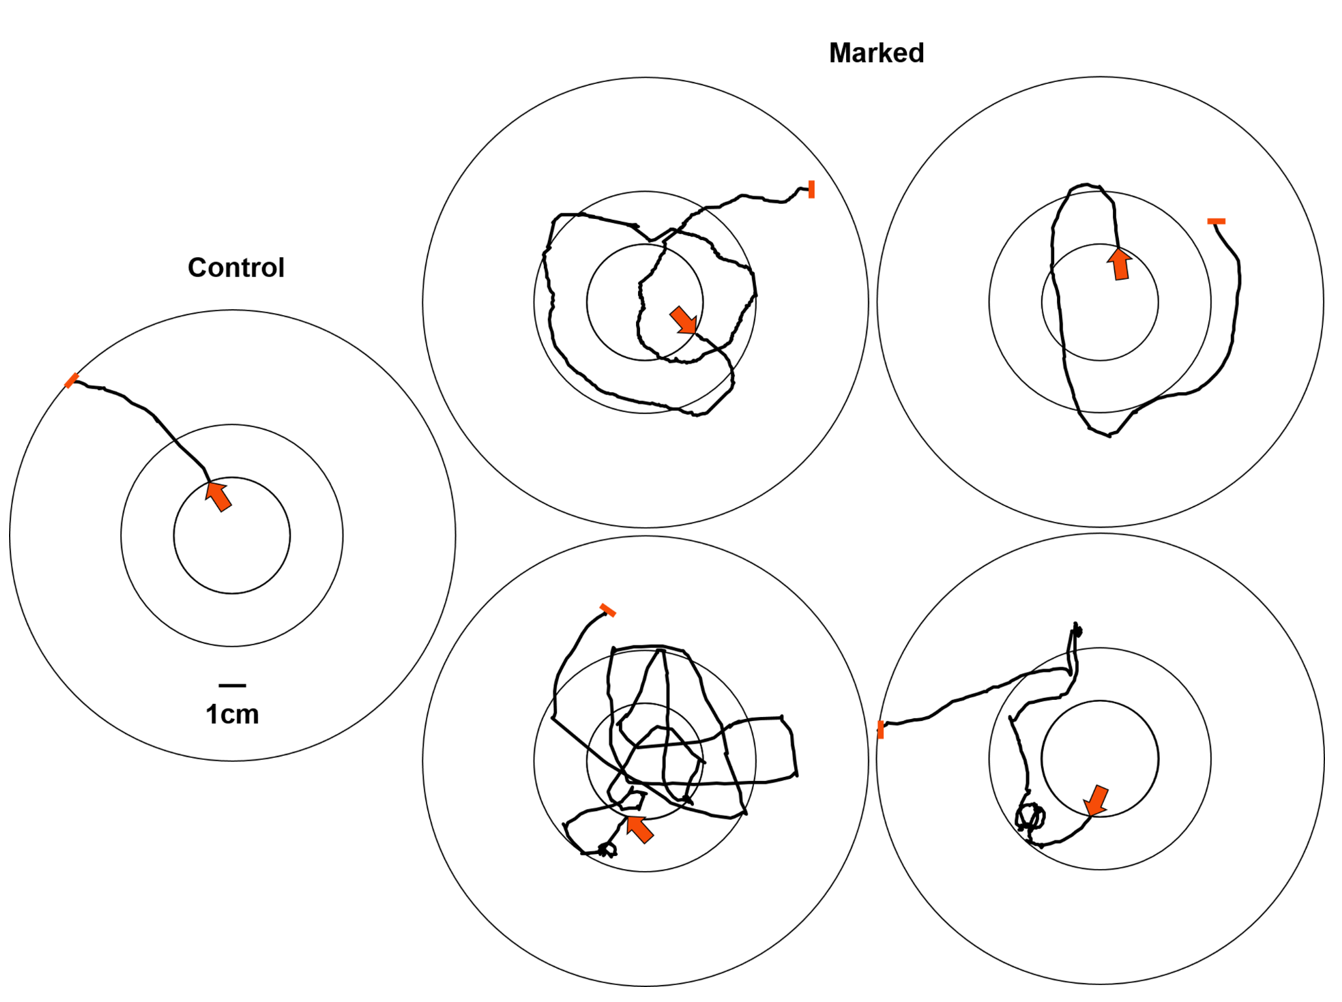
\includegraphics[width=0.9 \textwidth]{Figures/fig2.png}
		\rule{35em}{0.5pt}
	\caption[Trail]{Tracks of five \textit{Lucilia sericata} larvae during different attractive signal experiments (one Control and four Marked trials). The apparatus was comprised of three zones, a Centre Zone (the circle in the center), a Marked Zone (represented by the ring; marked by twenty starved larvae for 30 min; for Control trials this zone was unmarked), and an Outer Zone. The start point of each bioassay (trial) is represented by the arrow and the end-point by the small line. The trajectory pattern that was observed in the Control trials was the same for all of the other trials.}
	\label{fig:trail}

\end{figure}

\begin{figure}[ht]
	\centering
		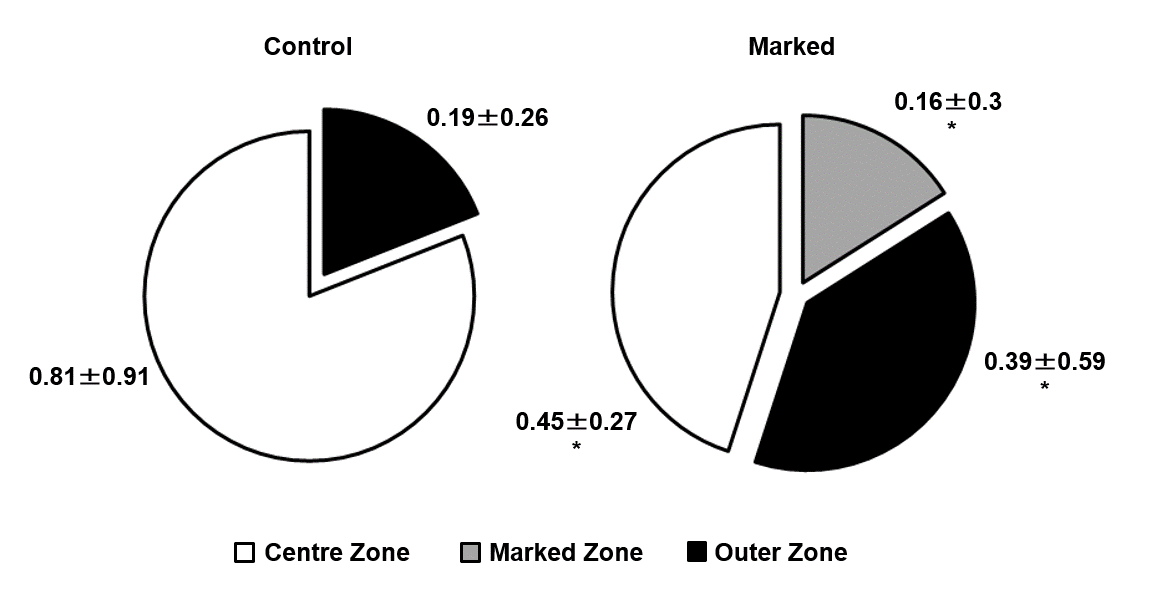
\includegraphics[width=0.9 \textwidth]{Figures/fig3.png}
		\rule{35em}{0.5pt}
	\caption[Proportion]{Mean proportion of time ($\pm$SD; n = 20) spent by \textit{Lucilia sericata} larvae in each of the behavioural trial zones. The asterisks (*) show significant differences between Control and Marked trials for each of the zones using bilateral tests \\(u$_{\alpha}$ = 1.96 for d.f. = 1).}
	\label{fig:proportion}
\end{figure}    
    
\clearpage

%----------------------------------------------------------------------------------------
%	SUBSECTION 3
%----------------------------------------------------------------------------------------   
			\subsection{Study of the scanning behaviour}  
The absolute meander was significantly higher in Signal conditions (Larvae, Food and Larvae + Food conditions) than in Control conditions, meaning that larvae had trajectories that were more tortuous when a signal was present in the arena (KW = 34.5, P $<$ 0.001). No significant differences were observed for the absolute meander between Signal conditions (Dunn’s tests: L vs. F: P $>$ 0.05; L vs. L + F: P $>$ 0.05; F vs. L + F: P $>$ 0.05).

The mean number of scanning movements varied according to test signals. Larvae scanned significantly more in the Control and Food conditions than in Larvae and Larvae + Food conditions (C vs. L: U = 81.5 P $<$ 0.01; C vs. L + F: U = 74, P $<$ 0.001; F vs. L: U = 121.5, P $<$ 0.05; F vs. L + F: U = 83, P $<$ 0.01; Figure \ref{fig:boxplot}). No significant difference was observed between the Control and Food conditions (C vs. F: U = 163.5, P $>$ 0.1; Figure \ref{fig:boxplot} ) and Larvae and Larvae + Food conditions (L vs. L + F: U = 142.5, P $>$ 0.1; Figure \ref{fig:boxplot}) again showing that scanning was decreased in the presence of the larval signal.

The larval signal also increased the time between two successive scannings: this time was significantly higher in Larvae and Larvae + Food conditions than in Control and Food conditions (C vs. L: U = 1341.5, P $<$ 0.05; C vs. L + F: U = 900.5, P $<$ 0.01; F vs. L: U = 1086, P $<$ 0.05; F vs. L + F: U = 728.8, P $<$ 0.01; Figure \ref{fig:boxplot}). As for the number of scans, the time between two successive scannings did not differ between Control and Food conditions (U = 2832.5, P $>$ 0.1; Figure \ref{fig:boxplot}) and between Larvae and Larvae + Food conditions (U = 585.5, P $>$ 0.1; Figure \ref{fig:boxplot}). 
The larval path clearly showed the places where individuals scanned (Figure \ref{fig:scan}). During their exploratory behavioural movements, larvae have intertwined locomotion and scanning (Figure \ref{fig:scan}). 
            
\begin{figure}[ht]
	\centering
		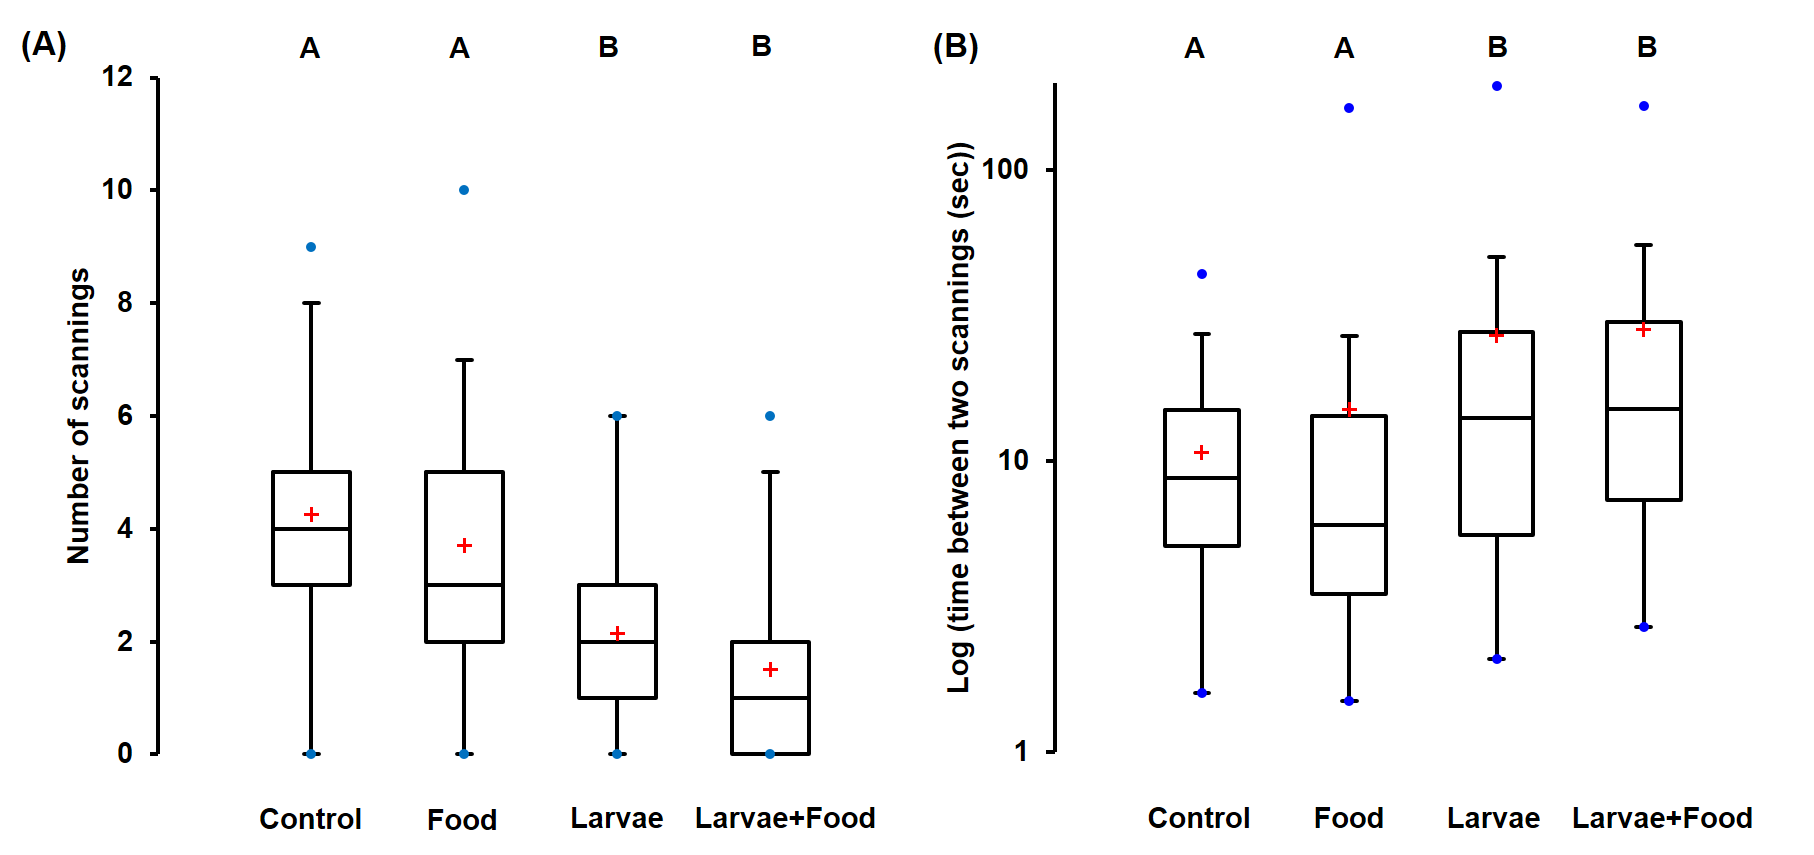
\includegraphics[width=0.9 \textwidth]{Figures/fig4.png}
		\rule{35em}{0.5pt}
	\caption[Boxplot]{(A) Boxplots of number of scannings performed by \textit{Lucilia sericata} larvae in each experimental conditions during the first minute of the experiment (n = 20, letters show significant differences in Mann-Whitney’s tests). (B) Boxplots of time (s) between two scannings of \textit{L. sericata} larvae in each experimental conditions during the first minute of experiment (n = 20, letters show significant differences in Mann-Whitney’s tests). Crosses represent the means.}
	\label{fig:boxplot}
\end{figure}

\begin{figure}[ht]
	\centering
		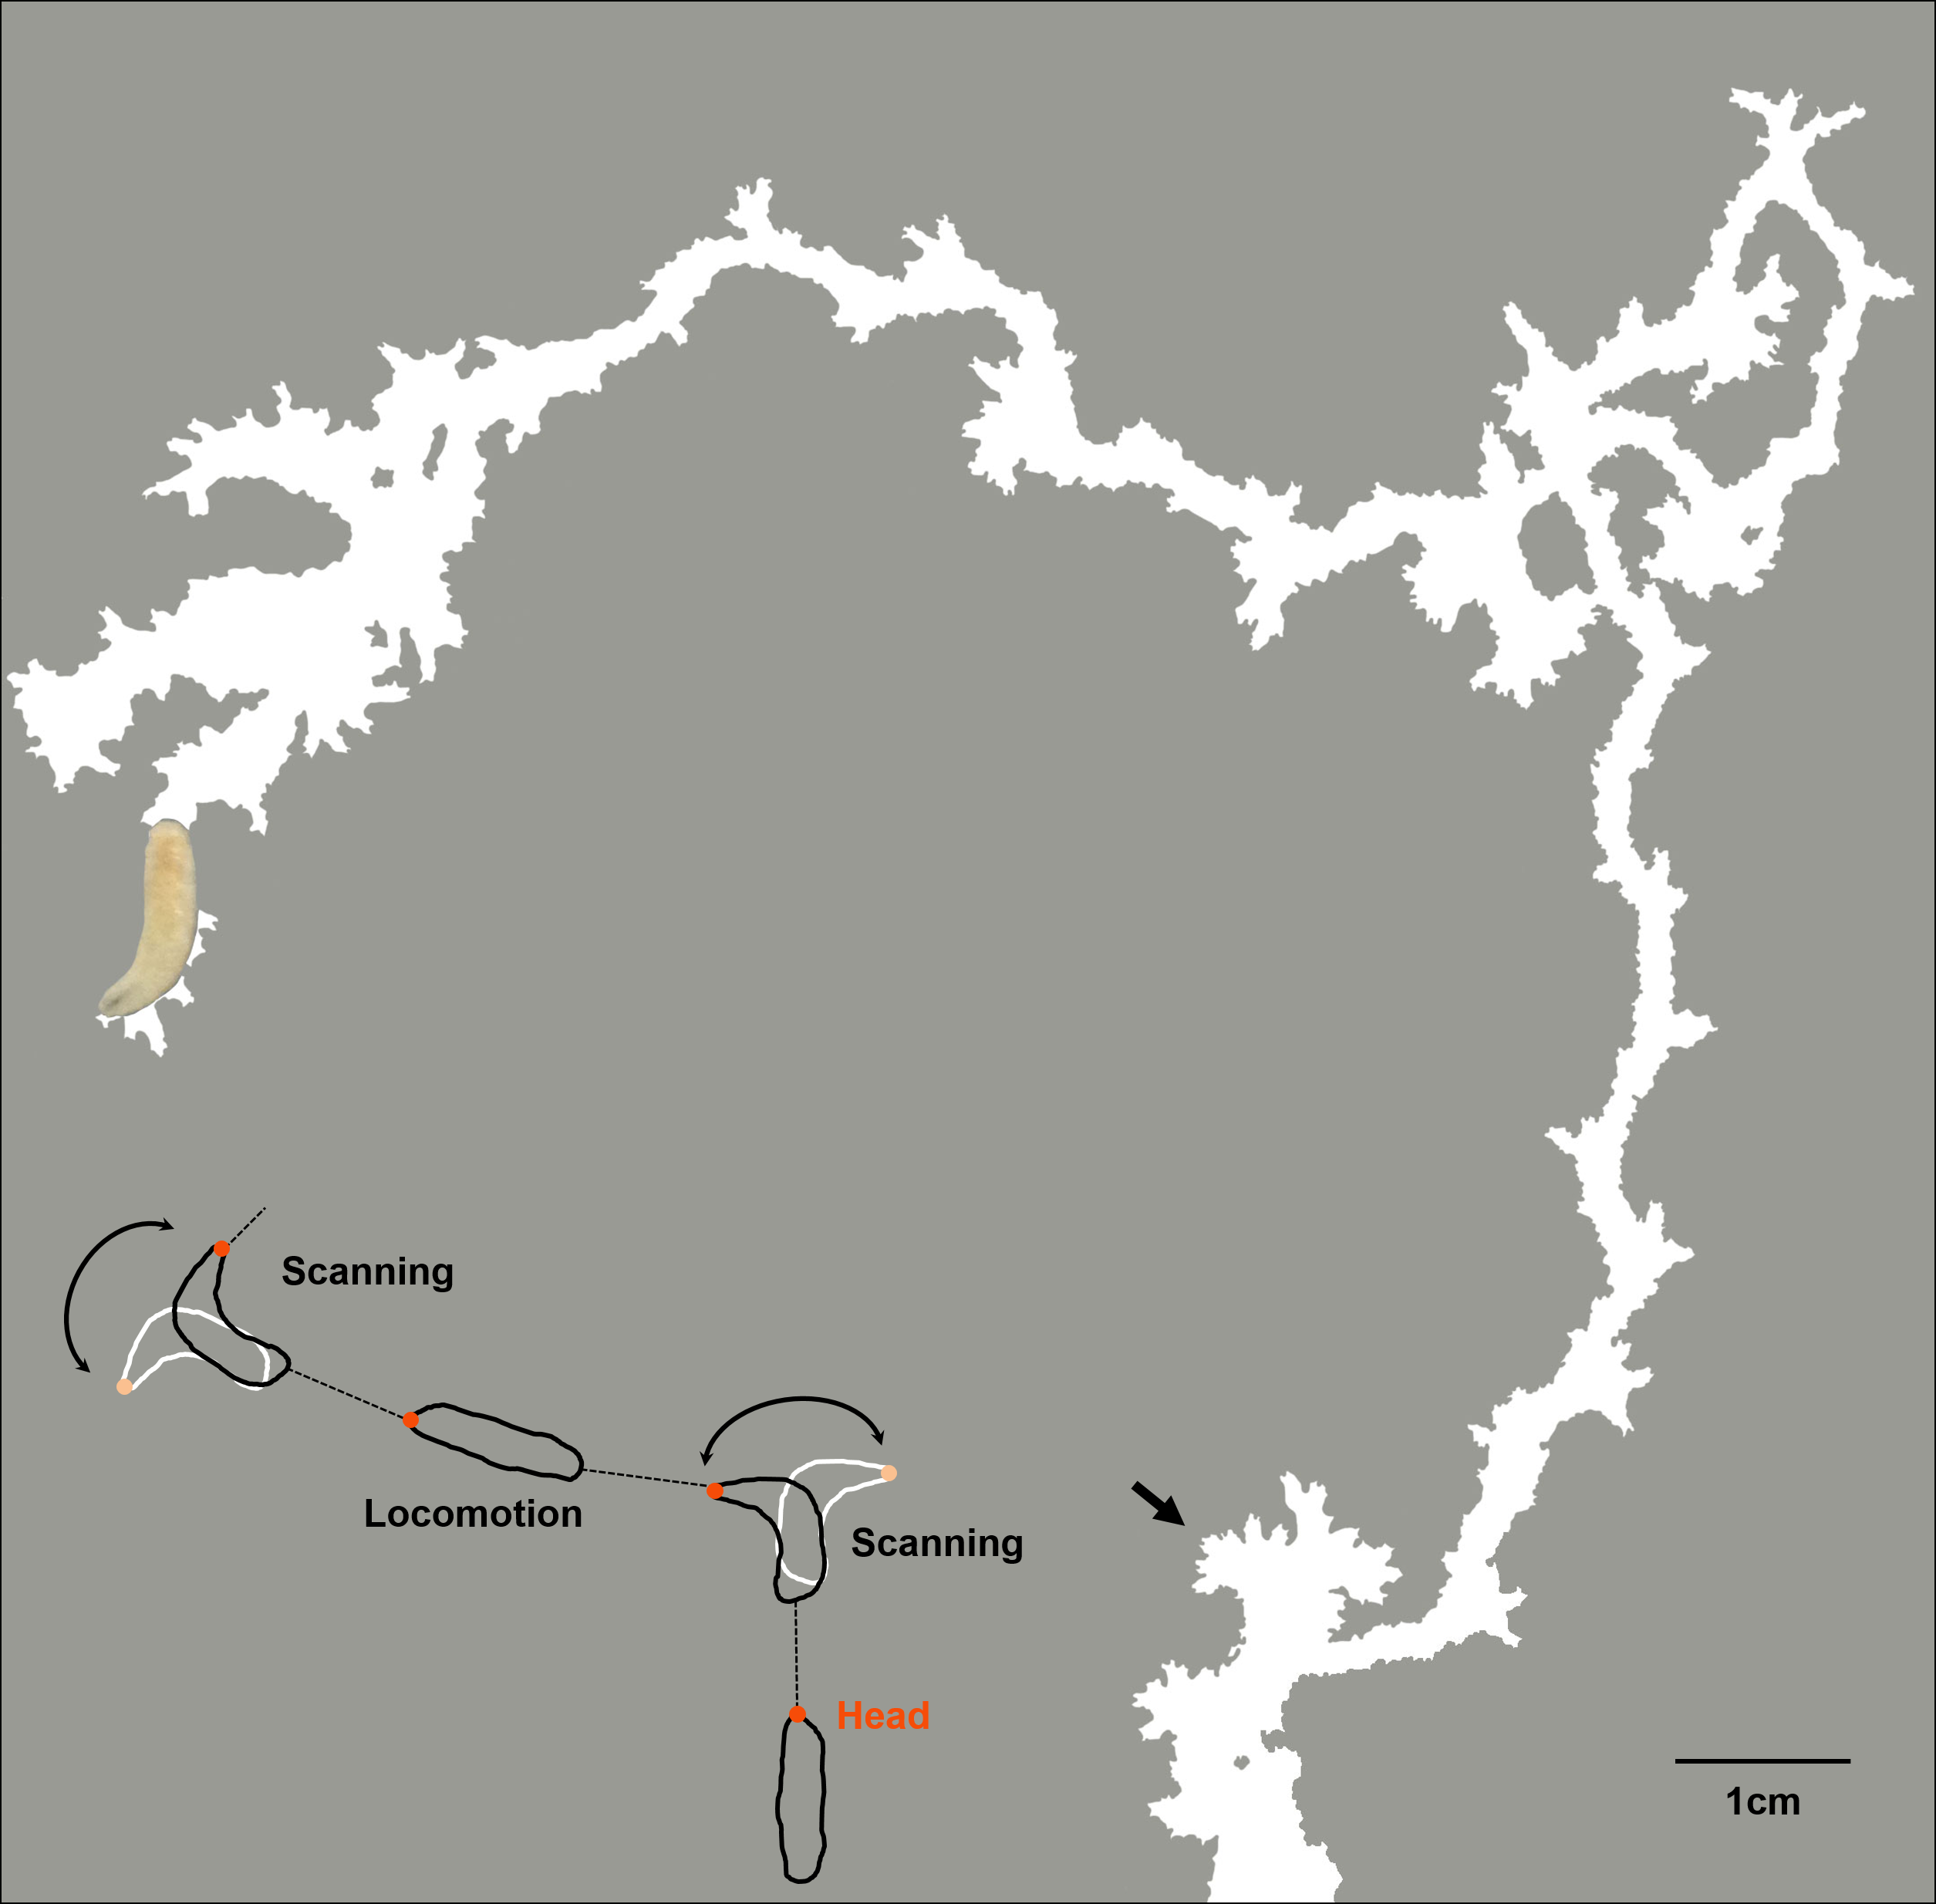
\includegraphics[width=0.6 \textwidth]{Figures/fig5.png}
		\rule{35em}{0.5pt}
	\caption[Scan]{A scheme of locomotion and scanning behaviour of \textit{Lucilia sericata} larva. During scanning, also named \textit{bending} \cite{green_organization_1983}, the larva is at the stop and successively turns the anterior third of its body on right and left directions. After few seconds scanning is over, the larva moves in the chosen direction. In white, the path of one \textit{L. sericata} larva in a new environment. The picture (modified from a photo) shows in white the area of physical contact between the larva and the substrate. The black arrow point one place where scanning occurred, with successive head position drawing a tree-like structure. Larva is visible at the left of the picture.}
	\label{fig:scan}
\end{figure}             

\clearpage           
%----------------------------------------------------------------------------------------
%	SECTION 5
%----------------------------------------------------------------------------------------
	\section{Discussion}   
    
%----------------------------------------------------------------------------------------
%	SUBSECTION 1
%----------------------------------------------------------------------------------------   
			\subsection{Limitations of the study}   
The authors are aware that this study does not definitely prove the implication of larval signal and scanning in aggregation of presocial larval blow fly. However, from the results obtained, it is reasonable to assume that the trail-following abilities of the larvae and the retentive effect of the 'larval signal' are involved in the aggregation process. Furthermore, although the exact role of scanning is not proven, there is a clear link with the presence of larval signal strongly implying a role in the aggregation behaviour.            
            
%----------------------------------------------------------------------------------------
%	SUBSECTION 2
%----------------------------------------------------------------------------------------   
			\subsection{Larval trail}
This study was designed to analyse the detection of a conspecific signals (as yet unidentified) by the necrophagous larvae of the Green bottle blow fly \textit{L. sericata} and to explore their signal-following abilities. Firstly, the results demonstrate that \textit{L. sericata} larvae are able to detect the boundaries of a signal left by conspecifics and their preference to stay within the prescribed area.  In the absence of signal from conspecifics, larval trajectories are straight with no about-turns. However, the prior presence of conspecifics (i.e., larval signal) impacts on the larval behaviour (Figure \ref{fig:trail}). Their trajectories are more sinuous, with numerous turns: larvae explore the arena instead of moving out of it (Figure \ref{fig:trail}). Accordingly, the \textit{L. sericata} larvae are able to detect a signal formerly left by conspecifics and alter their locomotion accordingly. A similar behaviour, based on biased running (very sinuous trajectories), has been observed during chemotaxis in Drosophila larvae \citep{gomez-marin_active_2011, gomez-marin_active_2012, ohashi_novel_2014}. This strategy is confirmed by regarding the branching tree-like path of \textit{L. sericata} larvae during an environment exploration (Figure \ref{fig:scan}). Larvae scan at each stop, turn slightly and continue their movement. The larvae are acquiring information about their environment (e.g., chemical gradient detection) by scanning, and are then moving accordingly.            
%----------------------------------------------------------------------------------------
%	SUBSECTION 3
%----------------------------------------------------------------------------------------   
			\subsection{Scanning behaviour}
The results show that \textit{L. sericata} larvae scan similarly in Control and Food conditions, but significantly less when a larval signal is present (Figure \ref{fig:proportion}). In both Control and Food conditions, the larval signal is absent: under these conditions, the larvae scan many times, and their successive scannings are close in time to each other. Such a scanning pattern is visible in Figure \ref{fig:scan}, which illustrates the result of numerous scans and changes in orientation. This finding agrees with that of \citet{green_organization_1983}, who observed no difference in the scanning frequency (called ‘bending’ in their study) of larval \textit{Drosophila melanogaster} between the food and no-food environments. On the other hand, individuals tested under Larvae and Larvae + Food conditions in the present study were directly in contact with the larval signal. They scanned for less time and less often. Accordingly, it is reasonable to assume that in \textit{L. sericata} larval scanning is involved in the detection of the chemical signal deposited by conspecifics on or in the substrate (i.e. klinotaxis; \citep{fraenkel_orientation_1961, gomez-marin_active_2012}). Further experiments will be required to identify the chemical composition of the larval signal (using gas-chromatography), and the involvement of the compounds identified in conspecific recognition (using behavioural tests). 

Aggregation of blow fly larvae is maintained by an active behaviour that is likely supported by a larval signal \cite{boulay_evidence_2013}. The detection of conspecific cues (tactile and chemical) is essential for larvae to be able to (re)join the group and to benefit from aggregation advantages \cite{rivers_physiological_2011}. The results presented here suggest that larvae use the scanning behaviour not only for turning but also to compare ground signals on either side (klinotaxis) and to orientate accordingly \cite{fraenkel_orientation_1961}. Larval masses are self-organized systems. One of the mechanisms of such social organization is the additive action of a signal that permits amplification of the system \cite{camazine_self-organization_2001}. According to the present observations and results, it is reasonable to conclude that scanning could be used by individual \textit{L. sericata} larvae to follow the trails left by conspecifics and/or to locate the most crowded areas. However, a precise description of the sensory organs of \textit{L. sericata} larvae and a demonstration of a direct linkage between these structures and the larval signal chemodetection are still needed. Such a linkage has already been explored for larvae of other dipteran species, such as \textit{Musca domestica} \citep{chu-wang_fine_1971, chu-wang_fine_1972}, \textit{Drosophila melanogaster} \cite{oppliger_neurophysiological_2000} and \textit{Hylemia sp.} \cite{honda_ultrastructures_1987}. 

%----------------------------------------------------------------------------------------
%	SECTION 6
%----------------------------------------------------------------------------------------
	\section{Acknowledgments}   
The authors would like to thank the two anonymous reviewers for their detailed and helpful suggestions. Authors also thank C. Devigne and J.L. Deneubourg (Senior Research Associate from the F.R.S.-FNRS) for their comments and M. Lemoine for photo editing.

\clearpage
    
    
            
            
            

% Chapter Template

\chapter{Interspecific shared collective decision-making in two forensically important species} % Main chapter title

\label{Chapter4} % Change X to a consecutive number; for referencing this chapter elsewhere, use \ref{ChapterX}

\lhead{Chapitre 4. \emph{Interspecific shared collective decision-making in two forensically important species}} % Change X to a consecutive number; this is for the header on each page - perhaps a shortened title

Julien \textsc{Boulay}\up{a,b}, Jean-Louis \textsc{Deneubourg}\up{b},  Valéry \textsc{Hédouin}\up{a} and \\ Damien \textsc{Charabidzé}\up{a}

\up{a} Univ. Lille, CHU Lille, EA 7367 - UTML - Unité de Taphonomie Médico-Légale, Lille, France\\
\up{b} Université Libre de Bruxelles, Unit of Social Ecology, Brussels, Belgium\\




Article resoumis à \emph{Proceedings of the Royal Society of London B}.


\cleardoublepage
%----------------------------------------------------------------------------------------
%	SECTION 1
%----------------------------------------------------------------------------------------
	\section{Abstract}
To date, the study of collective behaviour has mainly focused on intraspecific situations. Collective decision-making of mixed-species groups, involving interspecific aggregation-segregation, have received little attention. The study of such groups provides the opportunity to place the evolution of sociality in ecological and interspecific cooperation contexts. Here, we show that, in both conspecific and heterospecific groups, two gregarious larvae species were able to make a clear collective decision for one food spot. We observed similar dynamics between the two studied species: in both species, the choice was made within a few minutes and persisted throughout the experiment period. The monitoring of a focal individual within a group showed that these aggregations were governed by attractive and retentive effects of the group. The similarity observed between the conspecific and heterospecific groups suggested the existence of shared aggregation signals. These results can be characterized in larvae by a positive correlation between group size and heat generation; in the present study, the group size was found to have a stronger influence than the species of necrophagous larvae. This study provides the first experimental evidence of the dynamics of collective decisions-making in mixed-species groups of invertebrates, contributing to our understanding of the cooperation-competition phenomenon in animal social groups.

\textit{Keywords:} amplification – binary choice – gregariousness – marking – mixed-species group – tracking 

\clearpage

%----------------------------------------------------------------------------------------
%	SECTION 2
%----------------------------------------------------------------------------------------
	\section{Background}
To date, the study of collective behaviour has mainly focused on species with a high level of sociality \cite{costa_other_2006}. As a result, species with a lower level of social organization, such as those that exhibit gregariousness, have comparatively received little attention \cite{costa_other_2006}. However, the understanding of the key factors that permit the emergence of a collective decision in a large group composed of simple individuals (having a limited knowledge of their close environment) is fundamental to deciphering the evolution of sociality. Gregarism, which is observed in many species from mammals to unicellular species \citep{costa_other_2006,krause_living_2002,sumpter_collective_2009,parrish_complexity_1999}, can be defined as a gathering (i.e., an inter-attraction) of individuals independent of reproduction. Several insect species are gregarious at the larval instar and/or adult level \citep{costa_other_2006,jeanson_key_2012}. To find, form, stabilize or split aggregates, insects use various signals or cues (e.g., chemical, tactile and visual) \citep{costa_other_2006,krause_living_2002,sumpter_collective_2009,camazine_self-organization_2001}. In this context, the self-organization theory, independent of the nature of the interaction, has been successfully used to explain how simple interactions between individuals having only local information can generate a diversity of complex patterns at the collective level \citep{camazine_self-organization_2001,deneubourg_dynamics_2002,deneubourg_collective_1989}. It has been shown that consensus choices, called 'collective decisions' \citep{jeanson_key_2012,conradt_consensus_2005}, are made by various conspecific groups of insect species; a review on this topic was published by \citet{jeanson_key_2012}. Mixed-species groups are found in a large range of taxons from mammals \cite{stensland_mixed_2003} to birds \cite{farine_collective_2014}. Such groups offer identical benefits to those achieved by non-mixed groups, such as a protection from predators and efficient foraging behaviour \cite{costa_other_2006}. The existence of heterospecific groups raises the question of how sociality evolved in animals \citep{costa_other_2006,wilson_insect_1971}. ]. It also allows a discussion of new perspectives for livestock management to improve breeding conditions of species living together \cite{anderson_managing_2012}. Moreover, the existence of such groups suggests that similar, or close, aggregation cues are used by individuals regardless of species (cross-species recognition). Fewer studies have investigated heterospecific groups \cite{stensland_mixed_2003,farine_mixed-species_2014,diamond_mixed-species_1981}, particularly with regard to their collective decision-making abilities \cite{farine_collective_2014}. Some results regarding heterospecific associations in Diptera species have been reported in the context of species coexistence and competition \cite{dos_reis_larval_1999}, but no study has yet investigated the collective decisions of a mixed group from a quantitative point of view.\\
Aggregations of Diptera larvae, including heterospecific groups, have been extensively reported in the forensic entomology literature but remain poorly understood \citep{rivers_physiological_2011,charabidze_larval-mass_2011,boulay_evidence_2013,heaton_quantifying_2014}. Recently, \citet{boulay_evidence_2013} demonstrated that these aggregations are active and associated with chemical cues given by larvae of the blow fly \textit{Lucilia sericata}. \citet{rivers_physiological_2011} identified the benefits of maggot masses, such as heat generation, called the ‘larval-mass effect’ \cite{charabidze_larval-mass_2011}, and cooperation for the assimilation of food and digestion (increasing the local quantity of enzymes \cite{wilson_impacts_2015}). Regarding these benefits, aggregation behaviour facilitates cooperation and therefore permits an acceleration of larval development and increases in larval survival and carrion decomposition. Such benefits can be regarded as a source of the Allee effect \citep{courchamp_allee_2008,wilson_impacts_2015}.

The present study aimed to highlight the communal collective decision-making process of mixed-species groups leading to the choice of one food-spot. This study used \textit{L. sericata} and \textit{Calliphora vomitoria} larvae, two key species in forensic entomology that often feed simultaneously on carrion \cite{amendt_forensic_2004}. For this purpose, binary choice tests were performed between two identical food spots. The binary choice test has been used in several studies to highlight collective decision-making (see review in \citet{jeanson_key_2012}) and is also relevant to study necrophagous larvae (supplementary material, Figure \ref{fig:cochon}). Indeed, these species are often observed on symmetric cadavers, such as large mammals or rodents, which offer several identical spots for larvae to form groups on.
    
%----------------------------------------------------------------------------------------
%	SECTION 3
%----------------------------------------------------------------------------------------
	\section{Methods}
		\subsection{Insect rearing}
Larvae (maggots) were obtained from colonies bred at the Forensic Institute of Lille (Nord, France). Adult \textit{Lucilia sericata} and \textit{Calliphora vomitoria} were reared in separate cages at ambient temperature (20 $\pm$2\up{o}C) under daylight (12:12 h). The flies were fed caster sugar and water ad libitum. Upon the emergence of adult flies (day 0), minced beef liver was added for seven days (i.e., until day 7) to provide the protein required for vitellogenesis. After five days with no food, liver was again provided for use as an oviposition medium (day 12). After 24 h (day 13), eggs of \textit{L. sericata} and \textit{C. vomitoria} were separately placed on the breeding substrate (100 g of fresh minced beef liver). Larvae of \textit{L. sericata} were bred at 17$\pm$0.5\up{o}C, and after 5 to 6 days (day 18-19), young 3\up{rd}-instar larvae (10 $\pm$2mm in length) were sampled for the experiments \cite{grassberger_effect_2001}. Larvae of \textit{C. vomitoria} were bred at 20$\pm$0.5\up{o}C, and after 11 to 12 days (days 24-25), young 3rd-instar larvae (11 $\pm$2mm in length) were sampled for the experiments \cite{ames_low_2003}. The number of larvae used in each experiment (40) was sufficiently low to avoid autogenous heat emission (i.e., the larval-mass effect) \citep{charabidze_larval-mass_2011,heaton_quantifying_2014}.
    

		\subsection{Experimental setup}
The experimental arena consisted of an 18.5-cm-diameter Pyrex\up{®} glass Petri dish. The dish was filled to a height of 1 cm with agar-agar (7 g/250 ml) with two diametrically opposed food spots (5.5 cm in diameter), each situated 2 cm from the edge of the arena. These spots were designated as the west and east spots. Each spot consisted of a solution of liver (mean nutritional composition: 15.4$\%$ proteins, 7.3$\%$ carbohydrates and 4.1$\%$ fats (National Sanitary Security Agency)) and water (6 g/50 ml) mixed with agar. This food solution attracted a sufficient number of individuals and permitted clear counts of the number of individuals within each food spot, and each spot was sufficiently large to accommodate all of the larvae used in the trial (pers. obs.). Both food spots were strictly identical in size, composition and distance from the edge of the arena. The arena was placed in a climatic chamber (Firlabo) at 25$\pm$1\up{o}C and monitored by video.
	
    
		\subsection{Experimental procedure}
Before each trial, the larvae were removed from the feeding substrate, placed in wet pine-wood dust and isolated in the dark at 25$\pm$1\up{o}C for 1 h. This isolation time starved the larvae while the sawdust removed traces of food from their cuticles \cite{charabidze_discontinuous_2013}. Three conditions, including two conspecific conditions and one heterospecific condition, were tested: (1) 40 \textit{Lucilia sericata} larvae (N=30; conspecific condition), (2) 40 \textit{Calliphora vomitoria} larvae (N=30; conspecific condition) and (3) 20 \textit{L. sericata} + 20 \textit{C. vomitoria} larvae (N=30; heterospecific condition).


		\subsection{Conspecific condition and individual tracking}	
For each condition, forty larvae were randomly placed in a fresh arena in a dark room due to their high photophobic behaviour \cite{hinnemann_see_2010}. The arena was lit from below with a fluorescent neon light (8 W; Velopex) with a red ROSCO\up{TM} filter (ref. Roscolux $\sharp$19 Fire). This filter changed the spectrum of light by transmitting predominantly red wavelengths, which are not perceived by larvae \cite{hinnemann_see_2010}. The aggregation process was video-recorded over 60 min using a Bosch Dinion LTC0355 camera. The number of larvae in each of the three zones (the two spots and the area outside of the two spots) was counted visually at 1-min intervals. To be considered located outside of a spot, the individual had to have its entire bodies outside of the spot.\\
In each trial, a single larva was tracked throughout the 60-min trial period. To facilitate tracking, the selected focal individual was 1 mm longer than the other 39 individuals. Videos were down-sampled every 5 s (720 frames per video), and the position of the tracked larva was determined using Avimeca 2.7 freeware. The mid-point of the larval body was used for tracking. For the individual tracking analysis, we virtually enlarged the radius of each spot based on our tracking method (mid-point of the body) and the mean size of the individuals (10 $\pm$2mm). Such enlargement was set to 1 cm, corresponding to one larval body length increasing the radius from 2.25 cm to 3.25 cm.


		\subsection{Heterospecific condition}
Because the larvae of the two species are very similar in appearance, we marked the individuals according to their species to distinguish them during the heterospecific experiment. Twenty individuals of one species were marked using Lumicyano\up{TM} (Crime Scene Technology), a cyanoacrylate fluorescent glue that reacts to ultraviolet light \cite{prete_lumicyano:_2013}. The marking consisted of a small spot (1 mm\up{2}; Figure \ref{fig:lumi}) of Lumicyano\up{TM} placed on the anterior region of the larva’s dorsal surface. We used this glue to create UV-bright spots, thereby marking individuals according to species \cite{prete_lumicyano:_2013}. Lumicyano\up{TM} is very powerful and robust, dries quickly (2-3 s) and is available in several colours. These characteristics are useful for marking larvae with viscous cuticles and fast-moving species on which marking must be performed rapidly. Maggots are burrowing insects: they secrete a fat cuticular compound, crawl into cadavers and are often partially covered with decomposed flesh. In large masses composed of thousands of individuals, maggots move rapidly in a permanent turnover, creating high scramble competition \cite{rivers_physiological_2011}. These traits make it difficult or impossible to use the standard marking techniques for identifying and tracking insects \cite{hagler_methods_2001}. In a recent study, \citet{rosati_investigating_2015} successfully fed larvae with fluorescent fingerprint powders to obtain marked blowfly larvae. In the present study, in which the larvae were observed under dark and non-stress conditions, we developed an innovative, non-invasive marking method that allowed the tracking of larvae under UV light using a cyanoacrylate glue (Lumicyano\up{TM} \cite{prete_lumicyano:_2013}). Using this technique, we provide the first demonstration and quantification of a mixed-species aggregation with collective interspecific decision-making.\\
In contrast to the technique used by \citet{rosati_investigating_2015}, our method can be used with all blowfly larval instars and with other arthropod species (e.g., phytophagous taxa), and researchers can draw patterns or numbers to precisely identify individuals. This technique can also be used on several individuals simultaneously. Previous observations showed that the marking did not affect larval movement (test of aggregation with twenty marked individuals and twenty unmarked individuals in a monospecific condition; supplementary material, Figure \ref{fig:species}), and the marking was alternated between the two species before each trial. The arena was lit by two ultraviolet lights (2x15 W; Omnilux) because ultraviolet wavelengths are not perceived by larvae \cite{hinnemann_see_2010}. The aggregation process was video-recorded for 60 min using a 5-megapixel camera (GoPro Hero 3+\up{TM}, GoPro Enterprise). No individual tracking was performed during the heterospecific experiments due to the marking method and light conditions.

\begin{figure}[ht]
\centering
		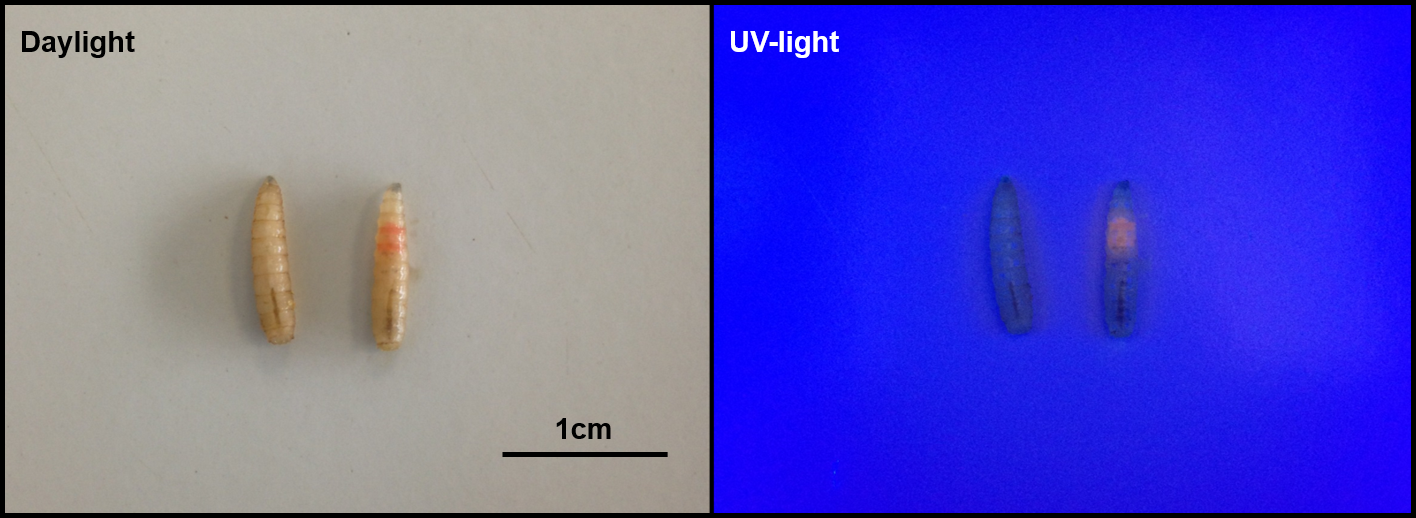
\includegraphics[width=0.8 \textwidth]{Figures/lumicyano.png}
		\rule{35em}{0.5pt}
		\caption[Lumi]{\textbf{\textit{Lucilia sericata} larvae, including non-marked larvae and larvae marked using Lumicyano\up{TM}}. For marking, a small spot of the cyanoacrylate UV-bright glue (1 mm\up{2}) was placed on the anterior part of an individual (on the larva’s crop).}
	\label{fig:lumi}
\end{figure}


		\subsection{Data analysis}
Trials resulting in an aggregation of individuals outside of either spot (denoted ‘outside trials’) were excluded from the analysis (corresponding to two trials of the \textit{L. sericata} group, four trials of the \textit{C. vomitoria} group and six trials of the heterospecific condition (mean proportion of outside trials: 13 $\pm$7$\%$). In total, 28 replicates were analysed for the \textit{L. sericata} group, 26 replicates were analysed for the \textit{C. vomitoria} group, and 24 replicates were analysed for the heterospecific group.\\
To verify that our setup was not biased for the left or right spot, we performed binomial tests. In support of the non-biased setup hypothesis, no side-related differences were observed between the two spots (west and east) during either the conspecific or heterospecific experiments (binomial tests for \textit{L. sericata}: p=0.16; for \textit{C. vomitoria}: p=0.18; for the heterospecific condition: p=0.17). Larvae did not choose one side of the arena more than the other one.\\
The spot with the largest number of individuals at the end of the experiment was designated the ‘Winner spot’, whereas the other spot was designated the ‘Loser spot’ (binomial test at t=60 min) \citep{halloy_social_2007,sempo_complex_2009}. To verify the neutrality of the setup, binomial tests were performed with the hypothesis H$_{0}$ assuming an equal distribution of individuals between the two spots (west and east). The data were tested for deviance from normality using the Kolmogorov-Smirnov test. Parametric tests were used if data normality and homogeneity of variance were observed; otherwise, corresponding non-parametric tests were used. The statistical tests were two-tailed and performed using GraphPad InStat 3.06 for Windows. All of the analyses assumed a significance level of $\alpha$ = 0.05, unless otherwise stated. For Dunn’s multiple paired comparison tests, the significance level $\alpha$ was adjusted using the Bonferroni method \cite{zar_biostatistical_2010}.


%----------------------------------------------------------------------------------------
%	SECTION 4
%----------------------------------------------------------------------------------------
	\section{Results}
		\subsection{Conspecific condition}
Of the 28 replicates performed with \textit{L. sericata}, we observed 20 replicates in which one food spot was preferentially chosen over the other at the end of the trial (binomial tests: p=0.01; supplementary material, Video S3). For \textit{C. vomitoria}, we observed 20 replicates out of 26 in which one food spot was preferentially chosen over the other (binomial tests: p=0.004; supplementary material, Video S4). On average, more than 50$\%$ of the individuals were found on the Winner spot (mean$\pm$SD; \textit{L. sericata}: 50.8$\pm$18$\%$; C. vomitoria: 57.2$\pm$14$\%$; Figure \ref{fig:choix}), whereas the Loser spot attracted less than 20$\%$ of the individuals (\textit{L. sericata}: 18.9$\pm$12$\%$; \textit{C. vomitoria}: 19$\pm$13$\%$; Figure \ref{fig:choix}). These percentages reflect a clear trend of collective choice for one spot (i.e., the Winner spot) by both species. Furthermore, the dynamics of these collective choices were similar between the two species. Each collective choice was made within 2 min of the start of the trial, with the majority of the individuals going to one spot (i.e., the Winner spot) (Wilcoxon tests at t=1 min Winner spot vs. Loser spot; \textit{L. sericata}, W=160, p=0.04;\textit{C. vomitoria}, W=189, p=0.003; Figure \ref{fig:choix}). In both conspecific conditions, these collective choices were made very rapidly and persisted throughout the trial period (Figure \ref{fig:choix}).


\begin{figure}[ht]
\centering
		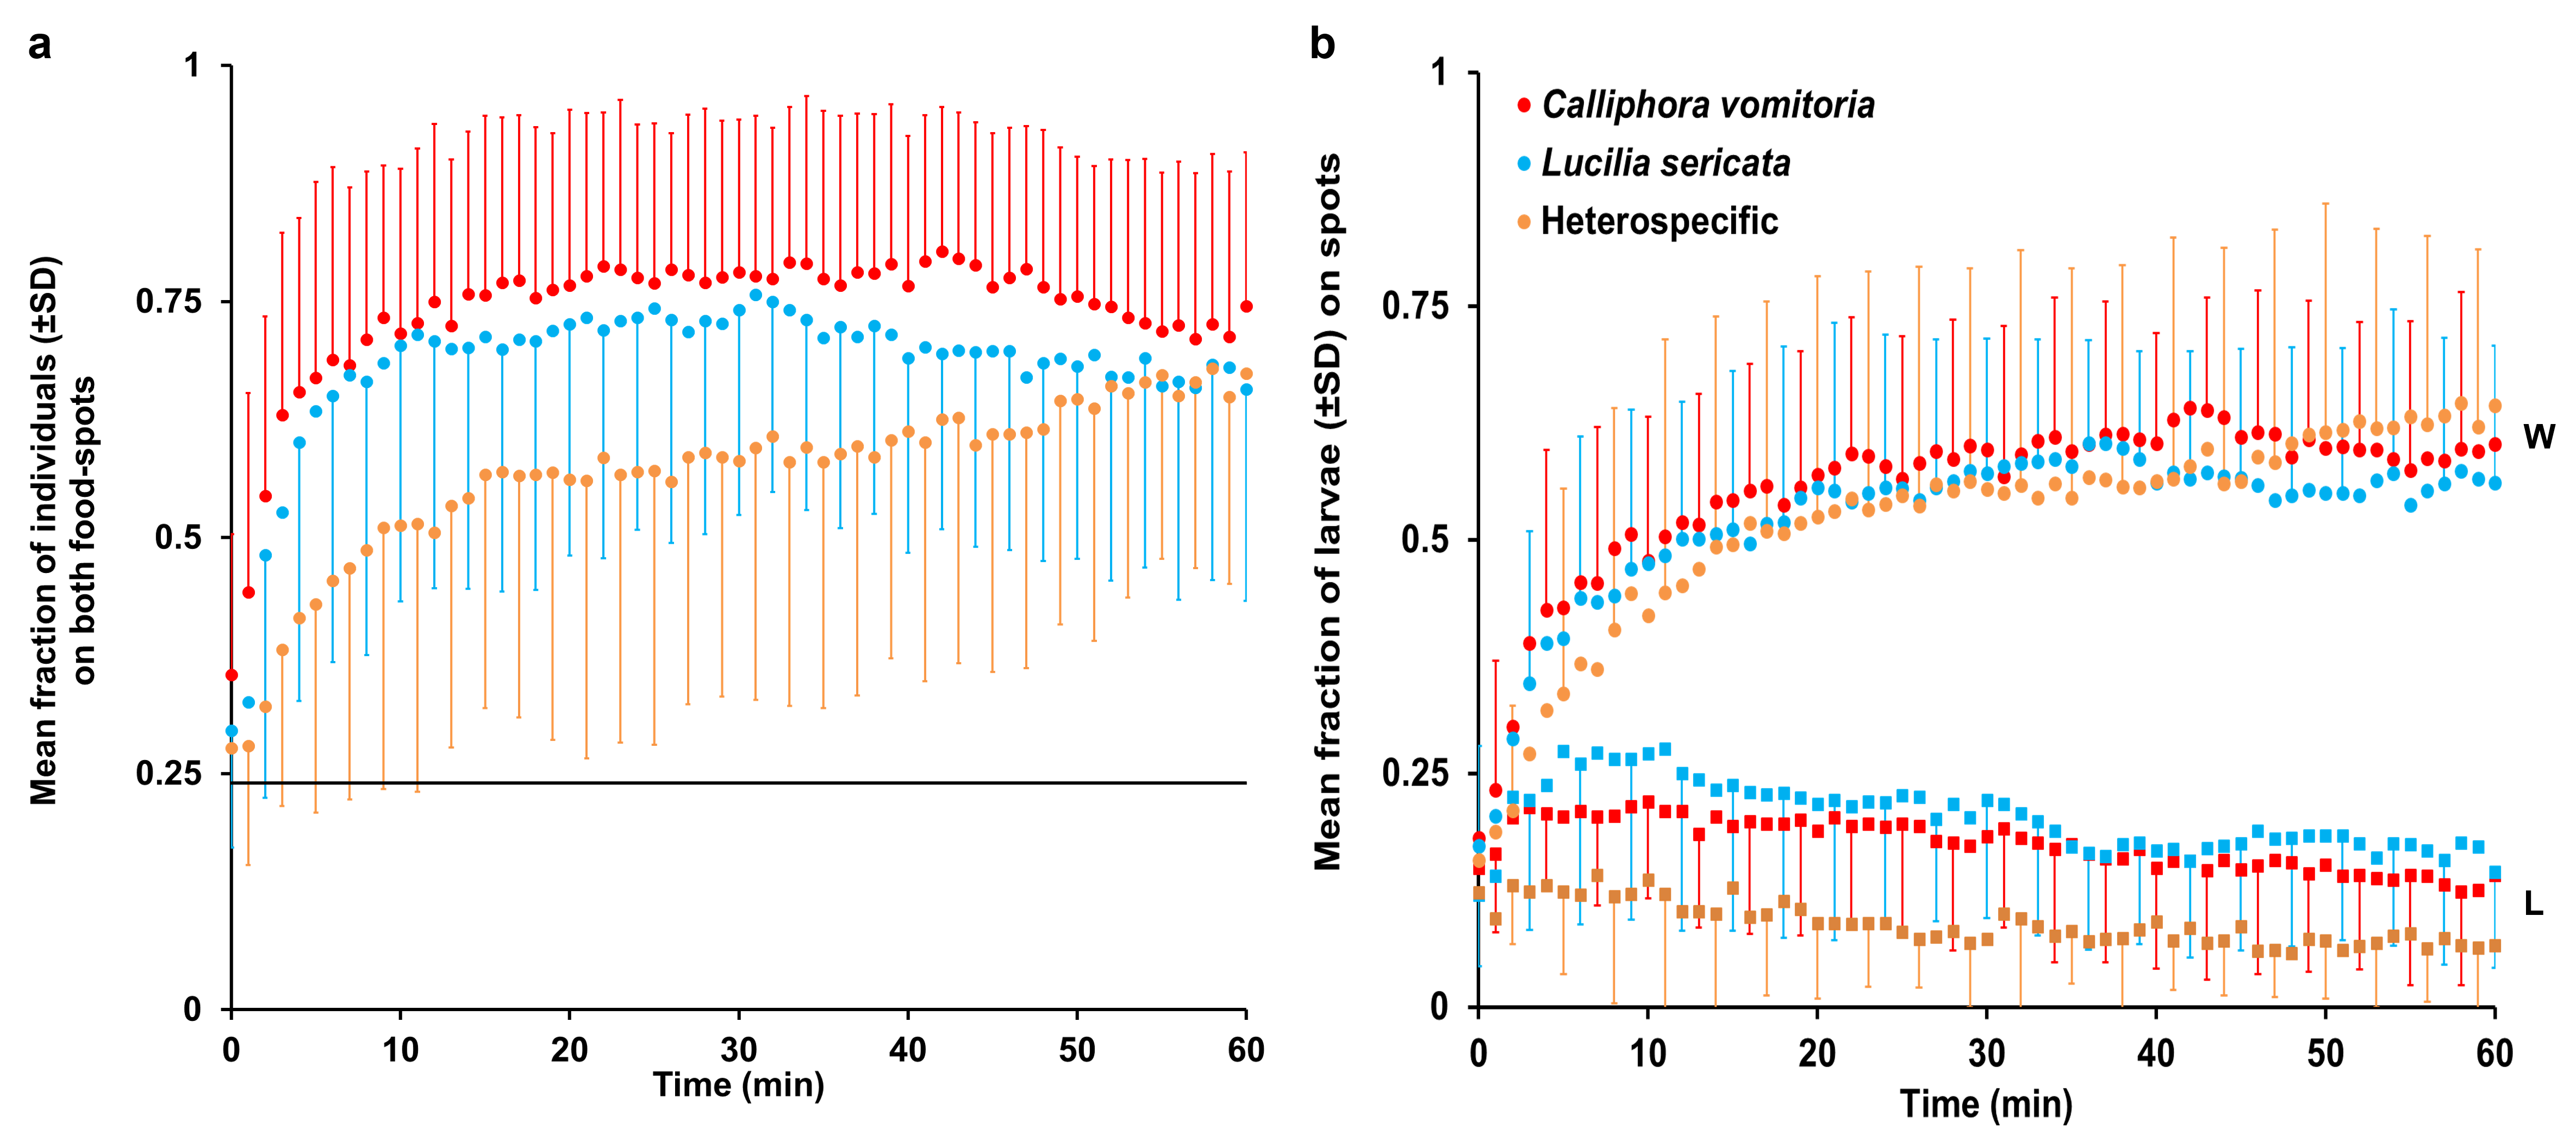
\includegraphics[width=1 \textwidth]{Figures/choix.png}
		\rule{35em}{0.5pt}
		\caption[Choix]{\textbf{Aggregation kinetics of conspecific and heterospecific groups}. \textbf{a}, Mean fraction of individuals in conspecific (\textit{Calliphora vomitoria} (red, N=26); \textit{Lucilia sericata} (blue, N=28)) and heterospecific groups (orange, N=24) on both food-spots over time. The horizontal line corresponds to a random distribution of individuals on the surface, which was calculated according to \citet{canonge_group_2011}. No differences were observed at t=0 min between a random distribution and the three observed distributions (bilateral tests: \textit{C. vomitoria}: u=1.37, p>0.05; \textit{L. sericata}: u=0.69, p>0.05; heterospecific group: u=0.42, p>0.05; $\text{u}_{\text{alpha}}$=1.96). Significant differences from a random distribution were observed 2 min after trial initiation for the \textit{L. sericata} groups, 1 min after trial initiation for the \textit{C. vomitoria} groups and 4 min after trial initiation for the heterospecific groups (using bilateral tests). The two monospecific kinetics presented no differences from t=0 min to t=60 min (Mann-Whitney tests). Multiple comparisons among the three conditions showed no significant differences from t=40 min (KW=5.12, p=0.08) to t=60 min (KW=2.48, p=0.29). Such comparisons showed that heterospecific groups aggregate more slowly than the two monospecific groups on both spots. \textbf{b}, Aggregation dynamics of 40 larvae in conspecific (\textit{C. vomitoria}, N=26; \textit{L. sericata}, N=28) and heterospecific groups (24 replicates; 20 individuals of each species). Mean fraction of individuals ($\pm$SD) found on the Winner spot (W; represented by circles) and the Loser spot (L; represented by squares). No differences were observed at t=60 min between the three conditions with respect to the Winner spot \\(KW=3.72, p=0.16) or the Loser spot (Dunn’s test, $\alpha$=0.017, p>0.05).}
	\label{fig:choix}
\end{figure}

		\subsection{Heterospecific condition}
In the 24 replicates performed with the two species together, we observed only three replicates in which no spot was preferentially chosen over the other. Of those trials yielding a clear choice of one spot, the two species chose the same Winner spot in 100$\%$ of cases (supplementary material, Video S5). The aggregation dynamics of the heterospecific groups were similar to those of the conspecific groups but required more time to join the plateau value of intraspecific groups (Figure \ref{fig:choix}). Indeed, at t=0 min, no differences were observed between the three conditions (KW=3.95, p=0.14; Figure \ref{fig:choix}). At t=2 min, the heterospecific groups were significantly different compared with the two monospecific groups (KW=14.96, p<0.001; Dunn’s test, $\alpha$=0.017, p<0.001; Figure \ref{fig:choix}). The heterospecific groups rejoined, in terms of the number of individuals, the two monospecific groups at t=40 min (KW=5.12, p=0.08), and this similarity lasted until the end of experiment (t=60 min, KW=2.48, p=0.29; Figure \ref{fig:choix}). These results show that the heterospecific groups aggregated more slowly on both spots than the two conspecific groups. The Winner spot contained more than 50$\%$ of the individuals (53.8$\pm$26$\%$; Figure \ref{fig:choix}), whereas the Loser spot attracted 8.1$\pm$7$\%$ of the larvae. On each spot, the number of larvae was balanced between the two species (e.g., Winner spot, t=30 min: \textit{L. sericata}: 10.1$\pm$5.6, \textit{C. vomitoria}: 10.1$\pm$5.5, t=0.72, p<0.001; Winner spot, t=60 min: \textit{L. sericata}: 12.0$\pm$5; \textit{C. vomitoria}: 11.5$\pm$5.1, t=15.2, p<0.001; Loser spot, t=30 min: \textit{L. sericata}: 1.4$\pm$1.6; \textit{C. vomitoria}: 1.7$\pm$1.7, t=4.3, p<0.001; Loser spot, t=60 min: \textit{L. sericata}: 1.1$\pm$1.3; \textit{C. vomitoria}: 1.9$\pm$2, t=3.7, p<0.001; supplementary material, Figure \ref{fig:species}). This result demonstrates that aggregation on the Winner spot was equally composed of both species over time, as determined based on the numbers of individuals.


		\subsection{Individual tracking}
The individual tracking of one larva during each trial was useful for understanding individual behaviour and how collective choice arises from larval displacements. The individual tracks showed that the larvae did not always remain on the Winner spot throughout the trials (Figure \ref{fig:tracking}). The larvae were highly mobile, moving back and forth on the Winner spot as well as exploring the Loser spot (Figure \ref{fig:tracking}). This observation was confirmed by analysing the mean duration of time spent on the Winner spot: larvae remained on it for only a short period of time (\textit{L. sericata}: 84.6$\pm$112 s; \textit{C. vomitoria}: 137.6$\pm$246 s; U=47308, p=0.03). However, foraging behaviour was clearly oriented toward the Winner spot; although this spot represented only 5.9$\%$ of the total test area, the mean time spent by the larvae on the Winner spot was 1616$\pm$750 s for \textit{L. sericata} and 1953.5$\pm$782 s for \textit{C. vomitoria}, representing 44$\%$ and 55$\%$ of the total experiment duration, respectively (bilateral test: u=0.63, $\text{u}_{\text{alpha}}$=1.96, p=0.49). Conversely, the larvae also remained on the Loser spot for a short period of time (\textit{L. sericata}: 46.4$\pm$76 s; \textit{C. vomitoria}: 84.4$\pm$209 s; U=11581, p=0.2). Individuals of \textit{L. sericata} spent 12$\%$ of the total experiment duration on the Loser spot (447.5$\pm$351 s), and \textit{C. vomitoria} individuals spent 15$\%$ of their time on this spot (552.8$\pm$808 s) (u=0.28, $\text{u}_{\text{alpha}}$=1.96, p=0.14). Positive relationships were observed between the time spent on the spots by the tracked individuals and the number of individuals present on the spot at this time (Figure \ref{fig:timenumb}). The larvae tended to stay longer on the Winner spot if the number of individuals already on the spot was high, suggesting a retentive effect of the group (Figures \ref{fig:timenumb} and \ref{fig:groupeffect}). Moreover, the time spent in the two other zones of the arena (Outside + Loser spot) tended to decrease as the number of larvae on the Winner spot increased (Figure \ref{fig:groupeffect}). Such results suggest the existence of an attractive effect of the group.

Additionally, the probability of returning to the Winner spot was higher than the probability of returning to the Loser spot for both species (the number of transitions from Winner-to-Winner was higher than that from Loser-to-Loser for both species; supplementary material, Figure \ref{tab:transition}). Moreover, the mean time to exit one spot and return to the same spot was shorter than that found for changing spots (supplementary material, Figure \ref{tab:transition}). These results are in agreement with the observation that larvae of the two species mostly moved near the edge of the Winner spot (Figure \ref{fig:tracking}) and reinforce the hypothesis of the existence of a retention effect of the group on the larvae (Figure \ref{fig:groupeffect}).

\begin{figure}[p]
\centering
		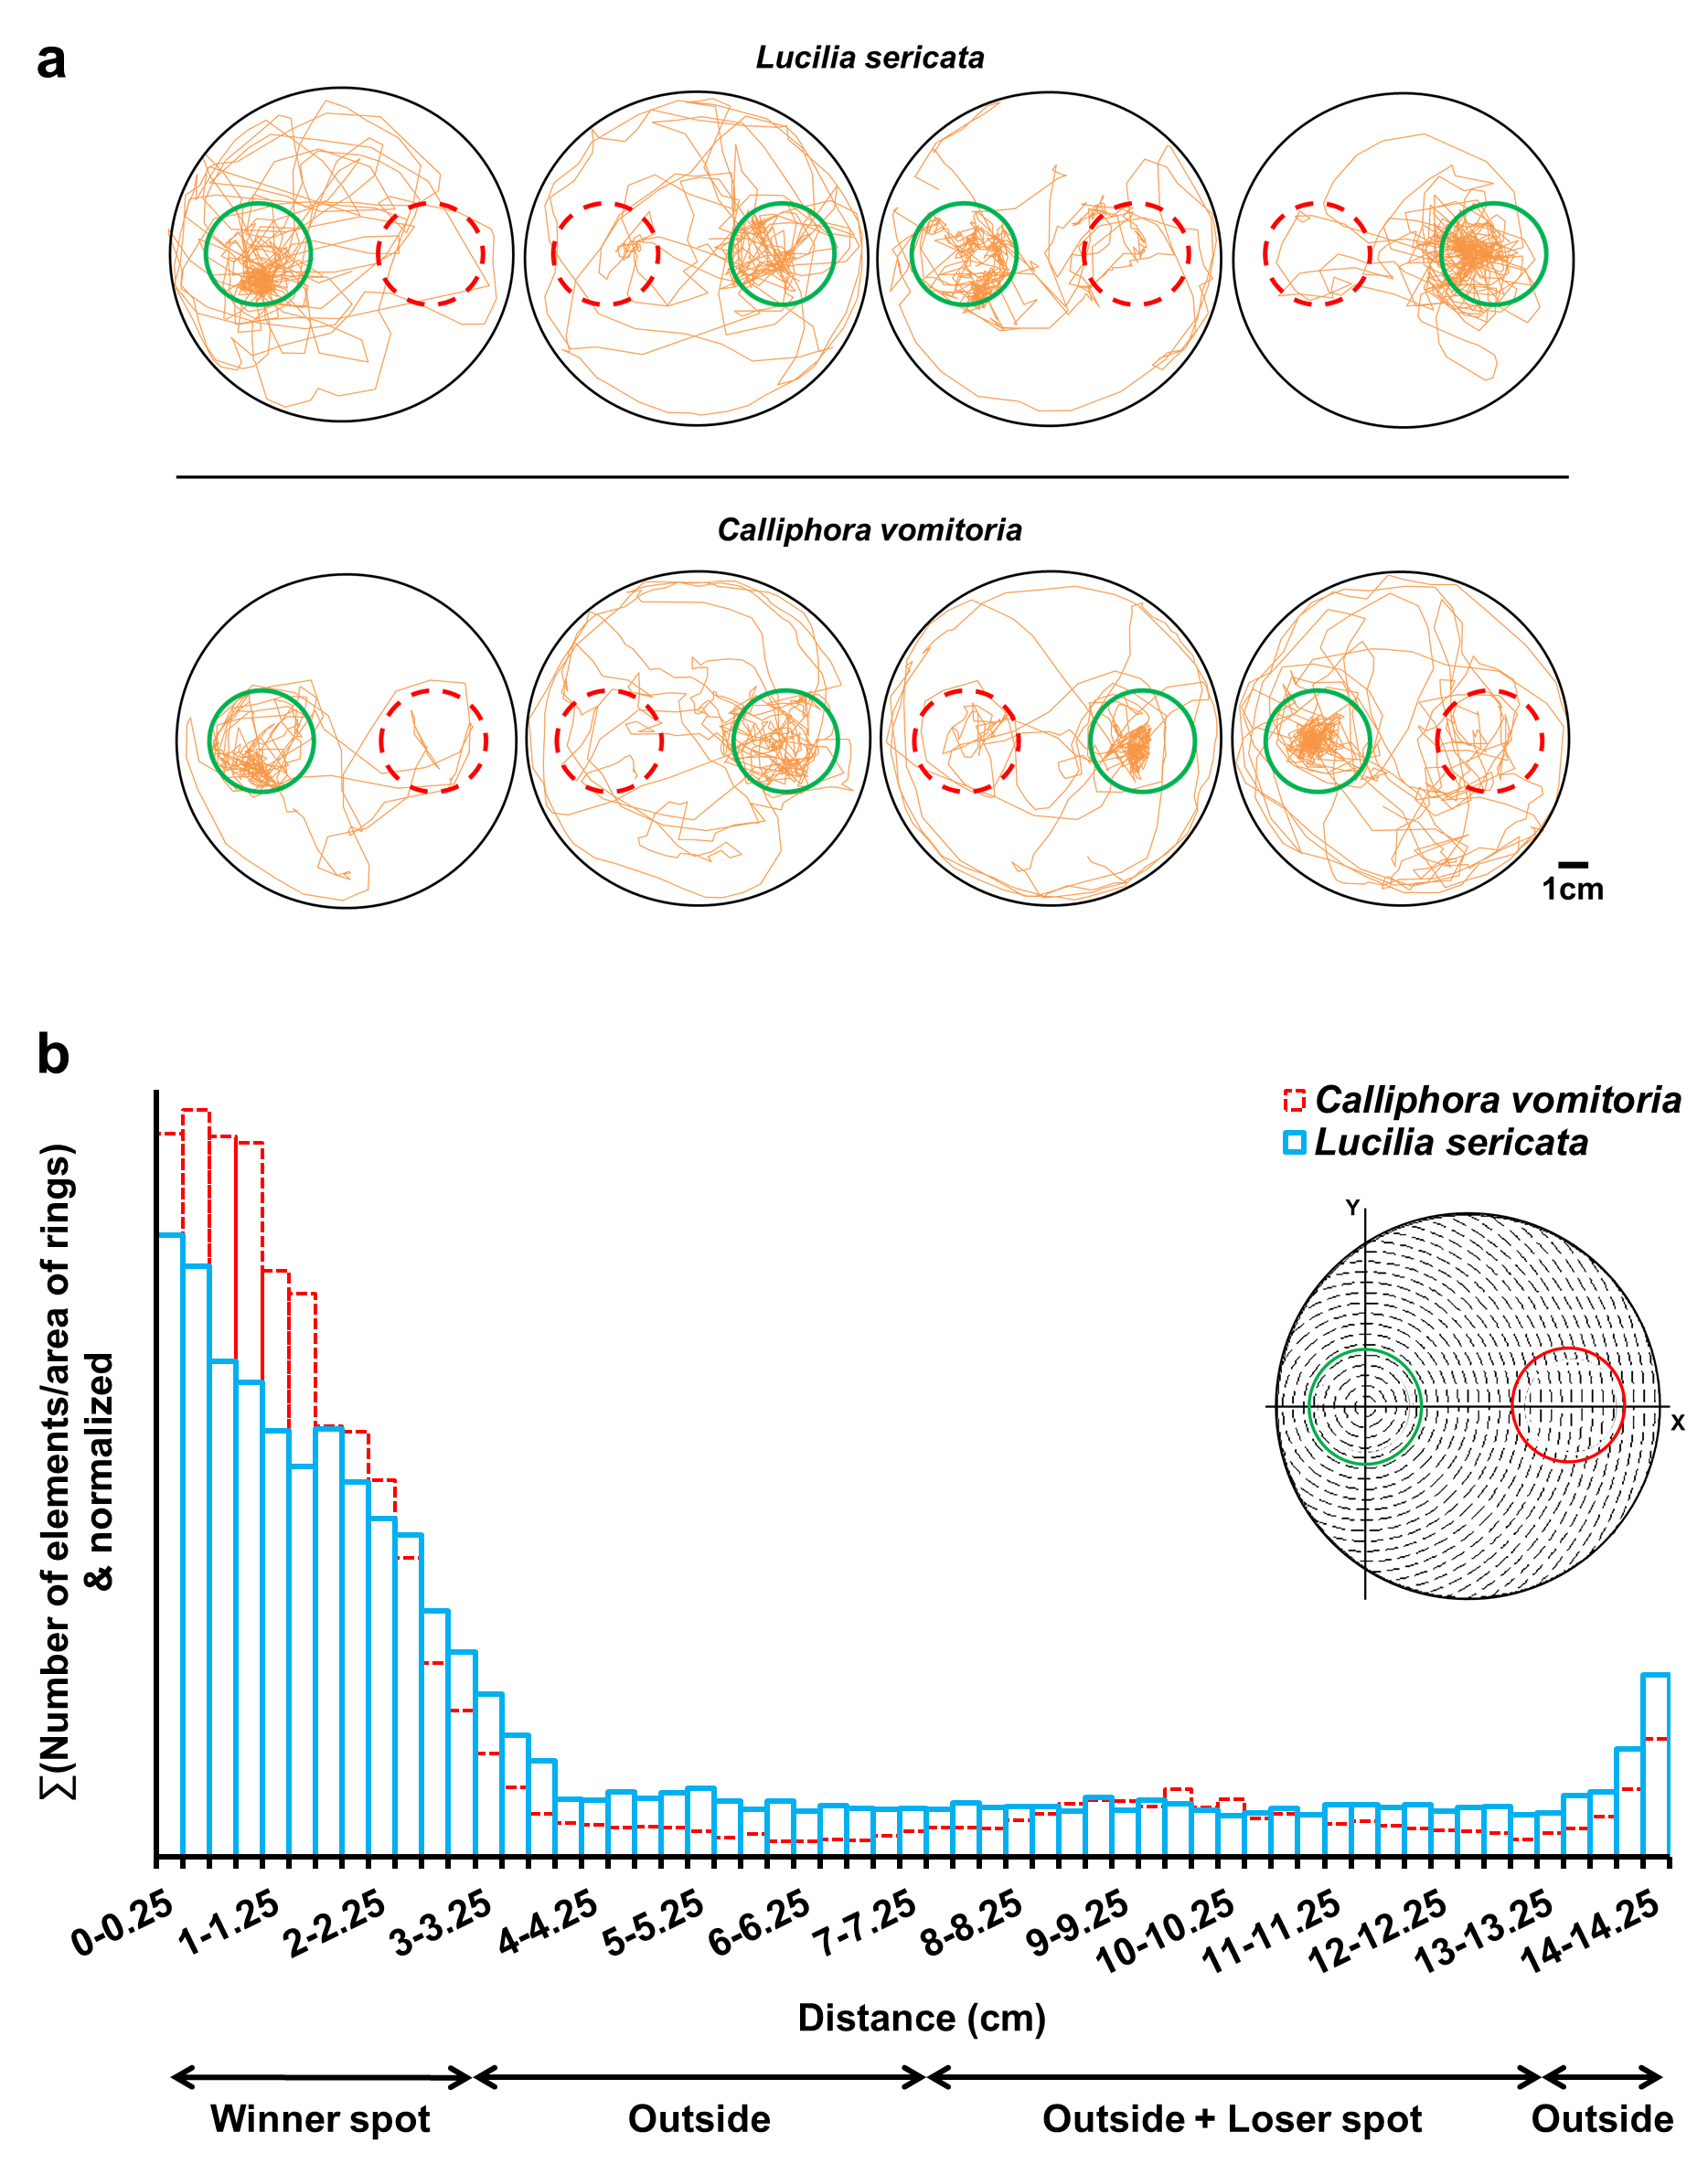
\includegraphics[width=0.8 \textwidth]{Figures/tracking.png}
		\rule{35em}{0.5pt}
		\caption[Tracking]{\textbf{Individual behaviour of larvae.} \textbf{a}, Tracks of eight larvae followed for 60 min during the conspecific experiment. The green circles represent the Winner spots, and the dotted red circles represent the Loser spots (diameter: 3.25 cm). \textbf{b}, Relative density of tracked larvae according to the distance (cm) from the centre of the Winner spot (conspecific experiments, N=20 for each species). The centre of the Winner spot was used as the reference coordinate (the Winner spot is represented by green, and the Loser spot is shown in red; diameter: 3.25 cm). The sum of the number of elements (distance to the centre of the Winner spot) divided by the ring area (see the illustration) is shown along the Y-ordinate axis.}
	\label{fig:tracking}
\end{figure}

\begin{figure}[p]
\centering
		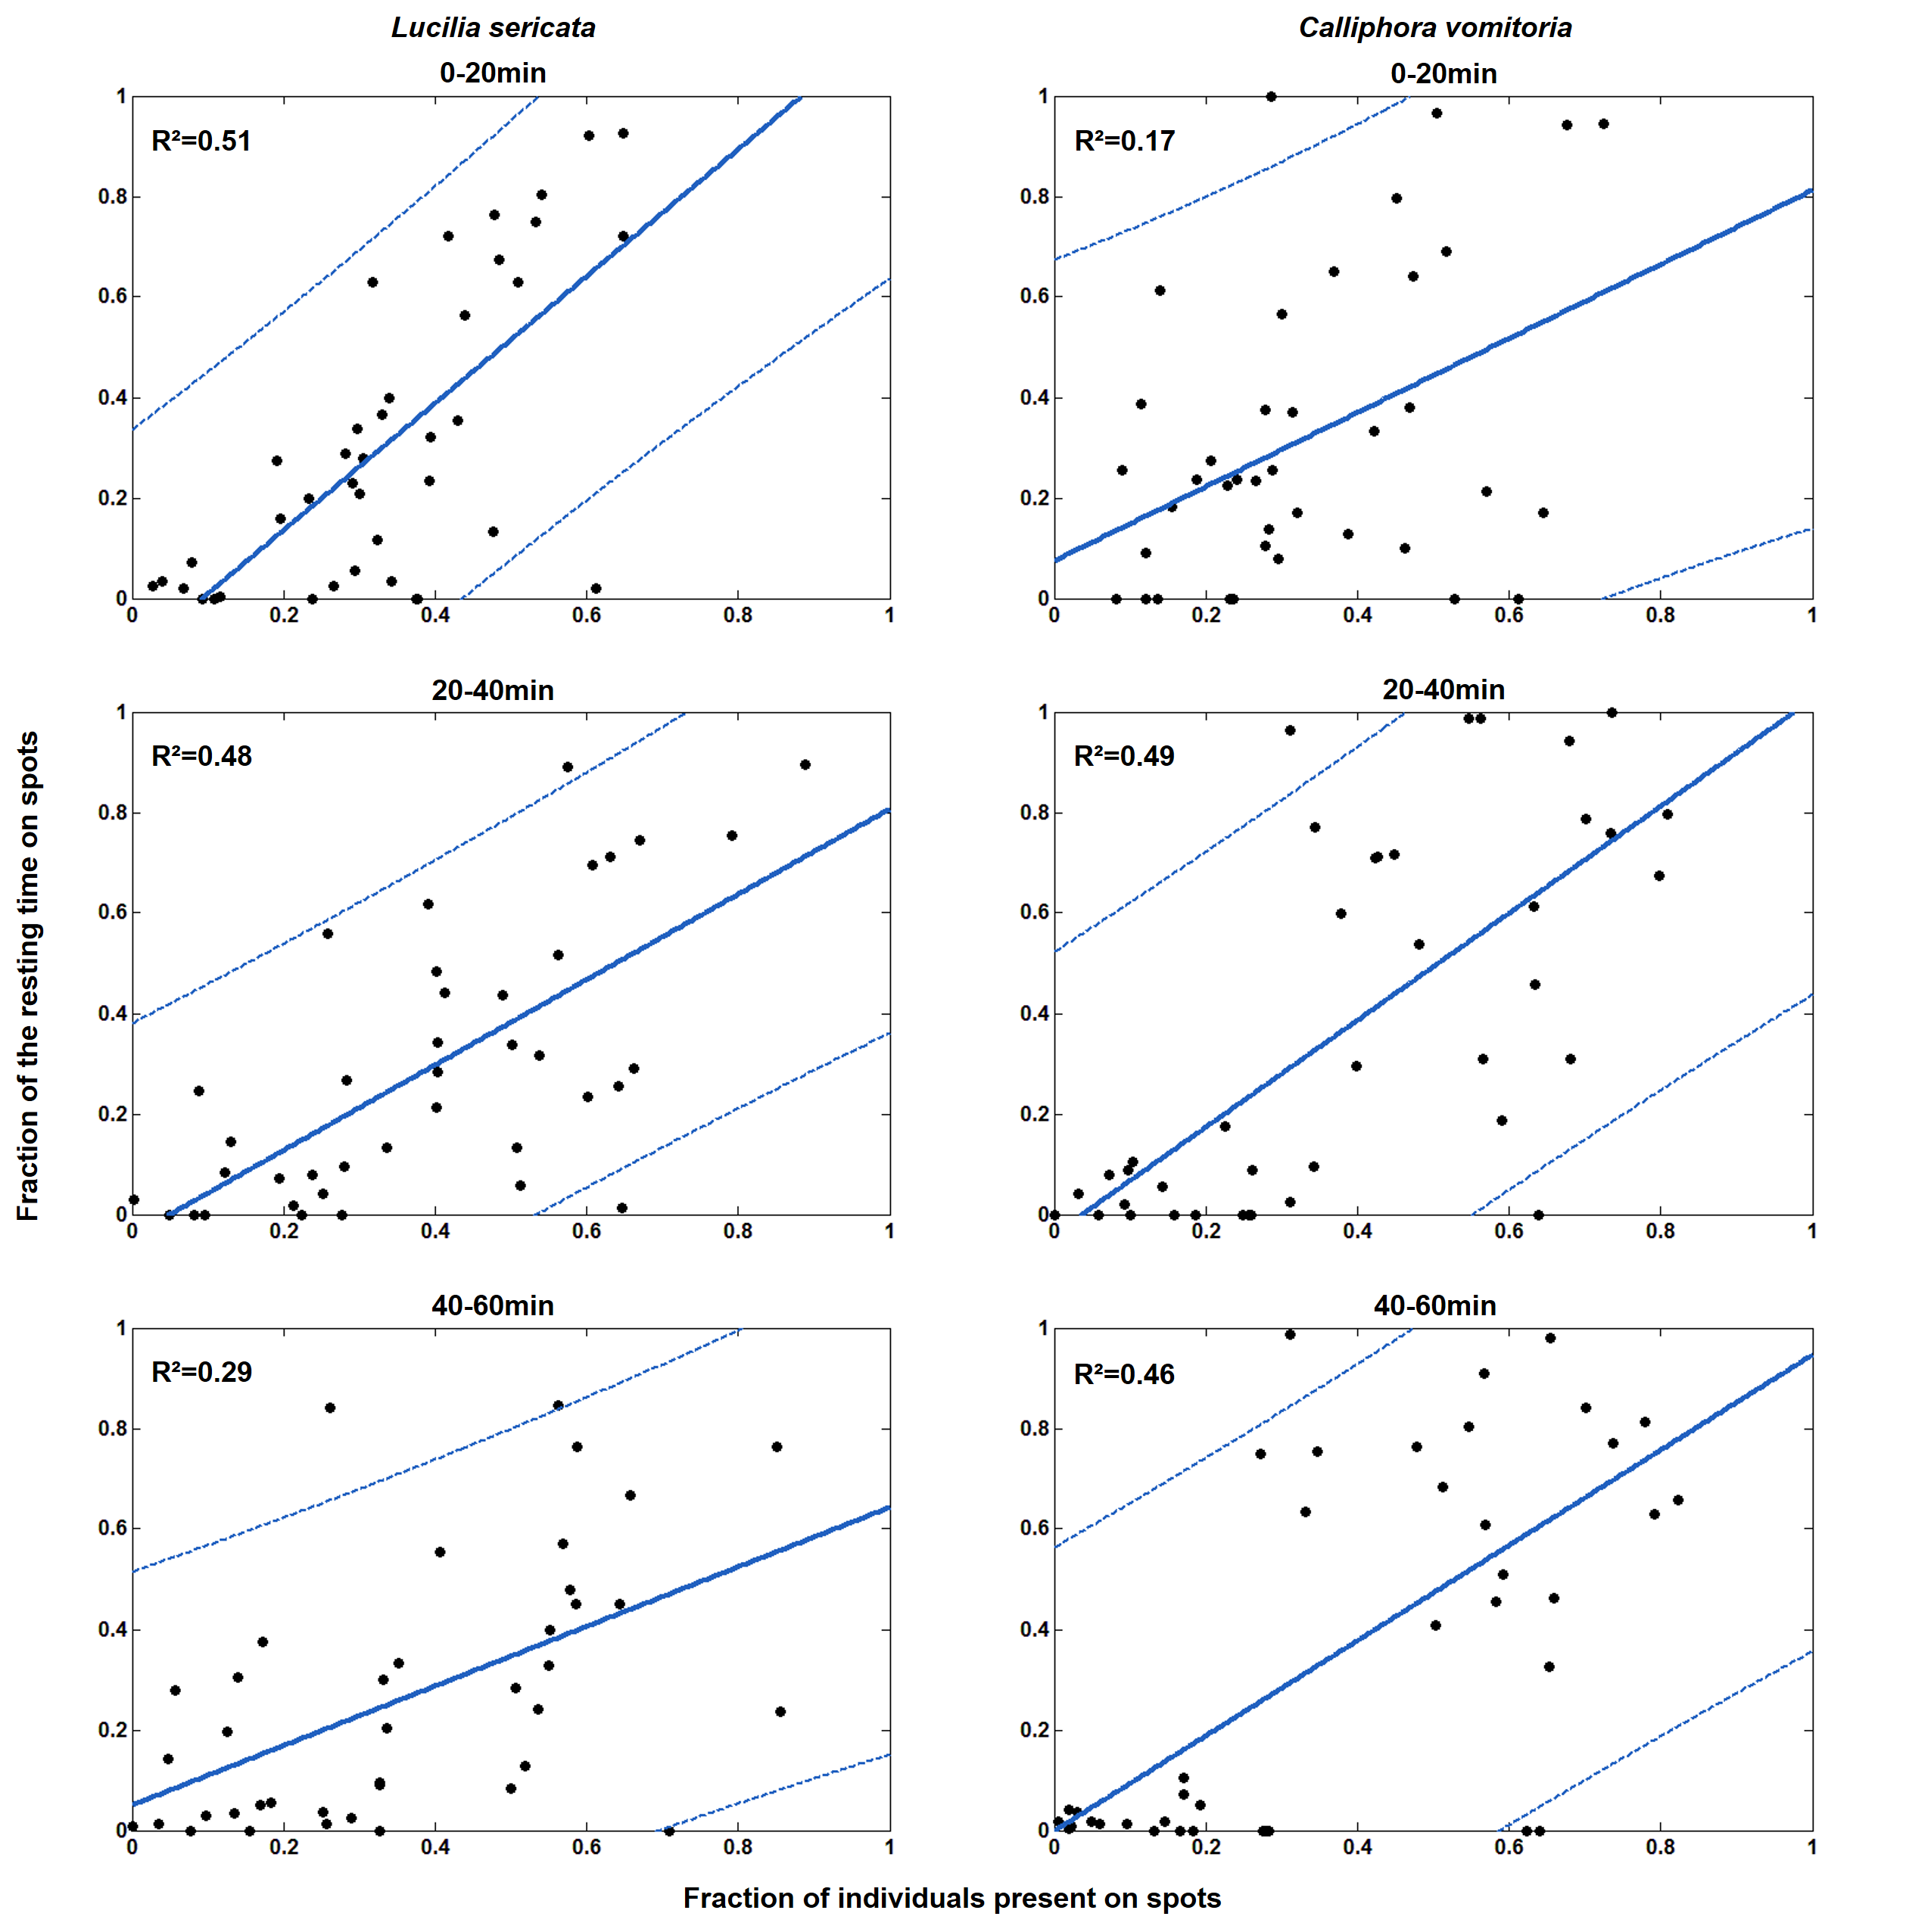
\includegraphics[width=1 \textwidth]{Figures/time_number.png}
		\rule{35em}{0.5pt}
		\caption[Timenumb]{\textbf{Time spent by tracked individuals on each spot according to the number of individuals present}. The trial duration was divided into three time periods. For each time period, the fraction of resting time on both spots (Winner and Loser) was plotted as a function of the fraction of individuals present on the corresponding spots. All of the linear regression slopes differed significantly from zero. \\The dotted lines correspond to the 95$\%$ CIs.}
	\label{fig:timenumb}
\end{figure}

\begin{figure}[p]
\centering
		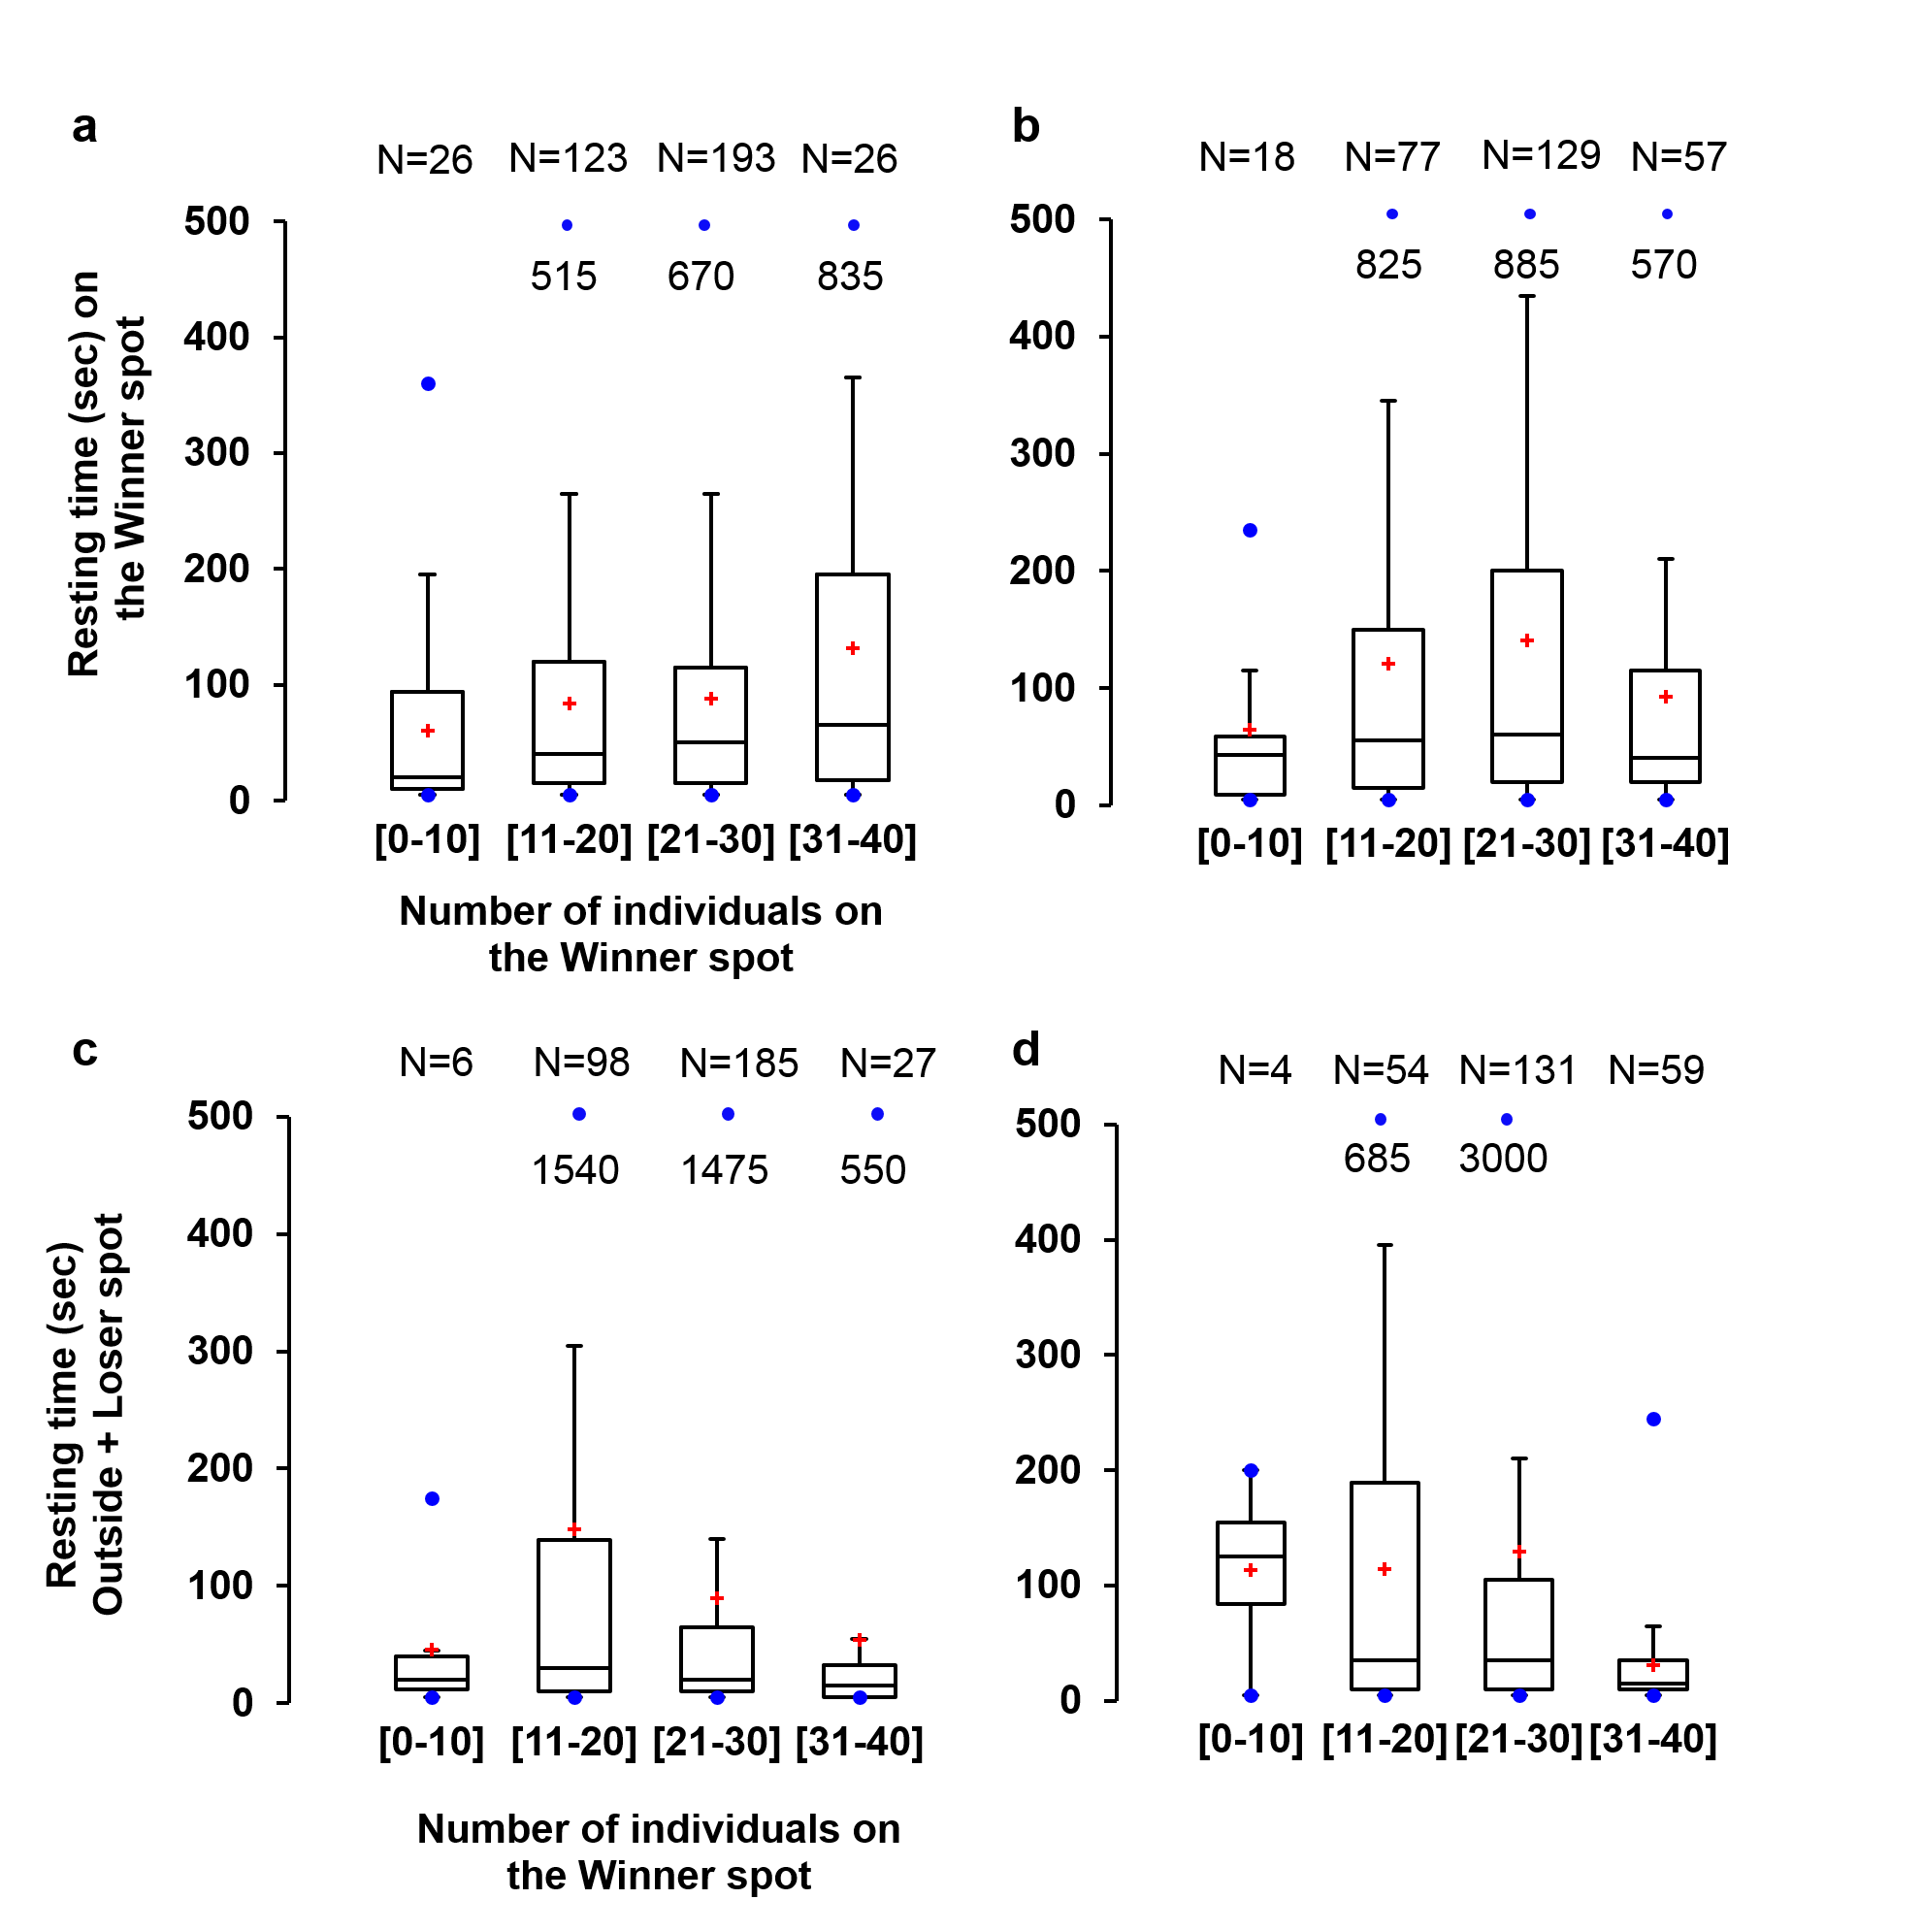
\includegraphics[width=1 \textwidth]{Figures/groupeffect.png}
		\rule{35em}{0.5pt}
		\caption[Groupeffect]{\textbf{Evidence of attractive and retentive effects of the group on individual larval behaviour.} Resting time (s) of tracked \textit{Lucilia sericata} larvae on the Winner spot (a) and Outside + Loser spot (c) as a function of the number of individuals on the Winner spot. Resting time (s) of tracked \textit{Calliphora vomitoria} larvae on the Winner spot (b) and Outside + Loser spot (d) as a function of the number of individuals on the Winner spot. For all boxplots, the first ten minutes were removed to reach a plateau regarding the accumulation of individuals on the Winner spot (Figure \ref{fig:choix}). No significant differences were observed in all boxplots according to the species (Kruskall-Wallis tests: 5a, KW=4.99, p=0.17; 5b, KW=4.77, p=0.17; 5c, KW=6.19, p=0.19; 5d (KW=13.73, p=0.003, Dunn’s test, p>0.05 for all multiple paired comparisons). The red crosses represent the means. N represents the number of elements. For trials in which aggregations were observed outside of either spot (\textit{L. sericata}, N=2; \textit{C. vomitoria}, N=4), the mean resting times of the individuals on the Winner spot were 75$\pm$112 s for \textit{L. sericata} and 17.9$\pm$13 s for \textit{C. vomitoria}. On the Loser spot, the corresponding times were 30$\pm$22 s for \textit{L. sericata} and 18.6$\pm$10 s for \textit{C. vomitoria}. The larvae spent less time on a spot when the number of individuals on the spot was low (means $\pm$SD throughout the experiment: Winner spot: \textit{L. sericata}: 6.8$\pm$3.5; \textit{C. vomitoria}: 2$\pm$1.5; Loser spot: \textit{L. sericata}: 3.7$\pm$4; \textit{C. vomitoria}: 2.4$\pm$2) (for comparison, see values in the text regarding trials yielding a collective choice for one spot).}
	\label{fig:groupeffect}
\end{figure}

\clearpage
%----------------------------------------------------------------------------------------
%	SECTION 5
%----------------------------------------------------------------------------------------
	\section{Discussion}
During the conspecific experiment, the majority of the larvae gathered on the food spots, and this distribution clearly differed from a random distribution (Figure \ref{fig:choix}). The collective choice of one spot, the Winner spot, out of the two spots occurred rapidly, within 5 min. The larval choice of one aggregation site is a consensus or collective decision \citep{deneubourg_dynamics_2002,conradt_consensus_2005}. The mechanisms underlying such collective decisions are self-organization and the use of local communication \cite{camazine_self-organization_2001}. Our individual tracking results showed that two mechanisms may be involved in this type of collective choice: the attraction and retention of the group (Figures \ref{fig:timenumb} and \ref{fig:groupeffect}). In blowfly larvae, this local communication likely involves a ground-marking signal that is passively left by crawling individuals; this larval signal has been shown to have an attractive/retentive effect on conspecifics \cite{boulay_evidence_2013}. The chemical profile of this cuticular signal has not yet been identified, but a recent study analysing the trail-following behaviour of blowfly larvae confirmed its existence \cite{boulay_first_2015}. Preliminary gas-chromatography results suggest that cholesterol could be one of the common signal for both species (Boulay, unpublished). According to the aggregation model presented by \citet{ame_collegial_2006}, it is likely that the larvae first explore the arena more or less at random but preferentially remain on food spots. Due to random asymmetry, the ground signal on one spot rapidly became stronger over time, which then created a Winner spot due to the progressive increase in the number of larvae on this spot. To support the hypothesis of the existence of this type of social amplification, simulation models, similar to those that have been used to investigate the self-organized collective decision-making process of cockroaches, will be constructed \cite{ame_collegial_2006}. The dynamics of aggregation was slower for the heterospecific group than for the conspecific group (Figure \ref{fig:choix}). Moreover, the mean number of individuals in the heterospecific group present outside the spots was greater than that found in the conspecific groups, whereas the mean number on the Winner spot was the same between the different groups, and the mean number on the Loser spot was lower in the heterospecific group (Figure \ref{fig:choix}). These results suggest the presence of a common retentive signal combined with a more species-specific attractive signal; moreover, these results suggest that the aggregation cues given by these two species are very similar and that at least one of the two species can detect and recognize the aggregation cues given by the other. However, a symmetric relationship in which the two species are able to recognize each other’s aggregation cues is possible.

In field conditions, various calliphorids larvae species are often observed in large aggregates composed of thousands of individuals of different instars and species. This strong aggregation behaviour is associated with an emerging property observed in large aggregates and commonly named the larval-mass effect \citep{charabidze_larval-mass_2011,slone_thermoregulation_2007}. The gathering of numerous larvae in dense masses can create a local increase in temperature that can reach 20\up{o}C above ambient. This modification of the thermal environment by larval groups decreases the duration of larval dependency on carrion (development time depends on temperature) and is considered one of the main benefits of gregarism in these species \cite{rivers_physiological_2011}. The cooperation observed between the two studied species is consistent with the Allee effect principle \cite{courchamp_allee_2008}. Aggregation behaviour allows larvae to reach a sufficiently large group size to receive benefits, such as heat generation and enzyme production \cite{rivers_physiological_2011}. Accordingly, heterospecific aggregation will allow larvae to reach this sufficient group size, particularly if the monospecific population is low. Such benefits can lead to an interspecific Allee effect. Our study highlights the importance of cooperative effects in blowfly larvae through the demonstration of active aggregation behaviour in conspecific and heterospecific groups. In natural conditions, full competition between larvae does not exist because each larval species has its own thermal preferences \cite{villet_contemporary_2010}. Conversely, segregation of two gathering species due to different thermal preferences has also been reported for closely related species \cite{villet_contemporary_2010}. Similar experiments should be conducted with more individuals, which will result in heat generation \cite{heaton_quantifying_2014}, and to study species segregation due to the specific thermal preferences of the larvae \cite{villet_contemporary_2010}. The notion of gregariousness often implies cooperation and/or competition. These two behaviours are the most fundamental principles that drive the evolution of social structures. The study of mixed-species groups offers biologists an interesting approach for exploring the frontiers between cooperation and competition in animal groups. Moreover, our results highlight that forensic entomologists should take into account the social behaviour of Diptera larvae, particularly the group size of larval masses, when estimating time of death.


	\section{Competing interests}
We have no competing interests.

	\section{Authors’ Contributions}
JB conceived of the study, design the study, collected data, carried out the statistical analyses, drafted the manuscript; DC conceived of the study, coordinated the study and helped draft the manuscript; VH gave final approval; JLD carried out the statistical analyses and helped draft the manuscript. All authors gave final approval for publication.   

	\section{Acknowledgments}
We thank the two anonymous reviewers for their very helpful comments. We thank F. Catteau for helping to track individuals. J.-L. Deneubourg is a Senior Research Associate from the F.R.S.-FNRS. 


%----------------------------------------------------------------------------------------
%	SECTION 6
%----------------------------------------------------------------------------------------
	\section{Supplementary materials}
    
\begin{figure}[h]
\centering
		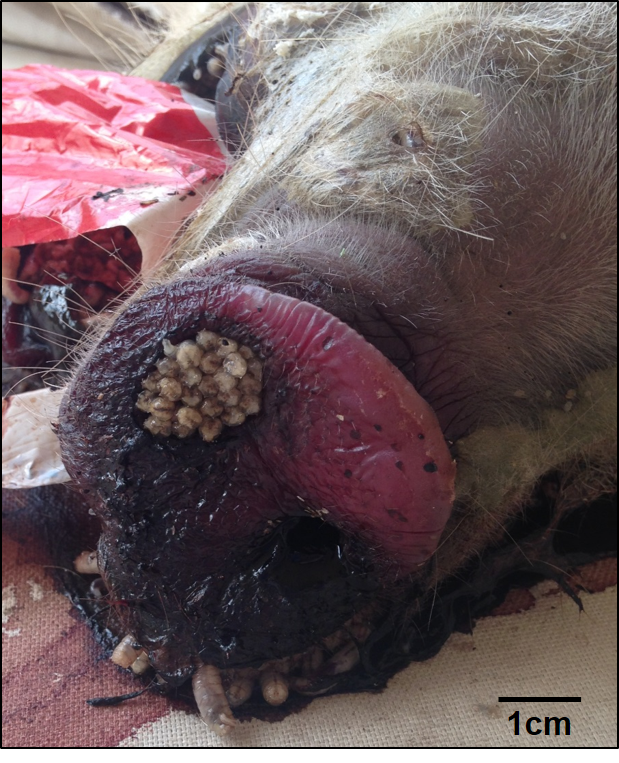
\includegraphics[width=0.5 \textwidth]{Figures/cochon.png}
		\rule{35em}{0.5pt}
		\caption[Cochon]{\textbf{Aggregation of necrophagous Diptera larvae on a pig cadaver (\textit{Sus scrofa}).} This aggregation was composed of Calliphoridae larvae and was located in a nostril (photo : J. Boulay).}
	\label{fig:cochon}
\end{figure}    

\begin{figure}[h]
\centering
		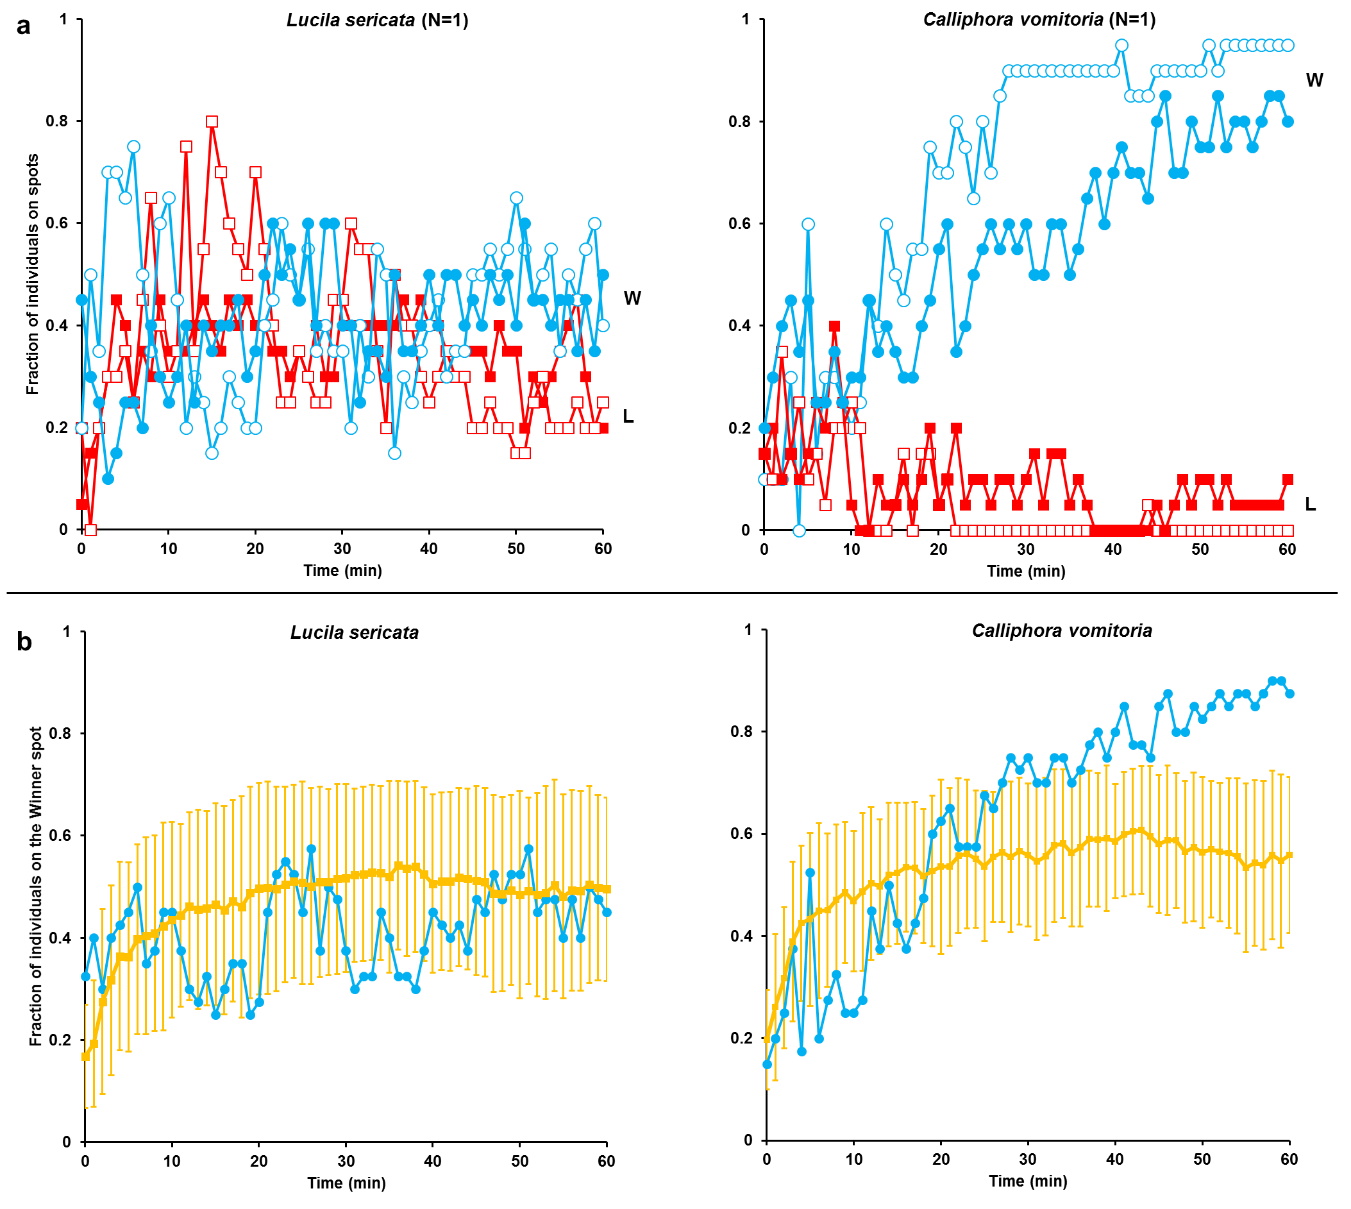
\includegraphics[width=1 \textwidth]{Figures/testagreg.png}
		\rule{35em}{0.5pt}
		\caption[Testagreg]{\textbf{Test of the effect of the marking technique on the aggregation of \textit{Lucilia sericata} and \textit{Calliphora vomitoria} larvae.} \textbf{a}, In this series of experiments, 20 larvae were marked using Lumicyano\up{TM} (filled dots) and 20 were not marked (white dots); an experiment was performed for each tested species, and collective choice for one spot was observed (Winner spot (W, blue lines); Loser spot (L, red lines)). For \textit{L. sericata}, the Winner spot sheltered 18 larvae, and the Loser spot had 9 individuals (binomial test: p=0.03). For \textit{C. vomitoria}, the Winner spot sheltered 35 individuals, and the Loser spot only had 2 (binomial test: p<0.0001). b, Fraction of individuals on the Winner spot during control experiments (in blue; sheltering marked and non-marked larvae) and during monospecific conditions (in orange; mean fraction ($\pm$SD) of non-marked individuals; seen in Figure \ref{fig:choix}). The marking method did not influence the aggregation dynamics of the intraspecific group composed by marked and non-marked conspecific individuals. Such results indicate that the marking technique used is non-invasive.}
	\label{fig:testagreg}
\end{figure}    

\clearpage

\textbf{Video S3. Collective choice of a \textit{Lucilia sericata} larvae group accelerated 20 times.} In green: the Winner spot; in red: the Loser spot. The focal individual was virtually marked by a white circle.

\textbf{Video S4. Collective choice of a \textit{Calliphora vomitoria} larvae group accelerated 20 times.} In green: the Winner spot; in red: the Loser spot. The focal individual was virtually marked by a white circle.

\textbf{Video S5. Collective choice of a heterospecific group accelerated 20 times.} Twenty \textit{Calliphora vomitoria} larvae were marked using the Lumicyano\up{o} and twenty \textit{Lucilia sericata} larvae were non-marked.
\\

\begin{figure}[h]
\centering
		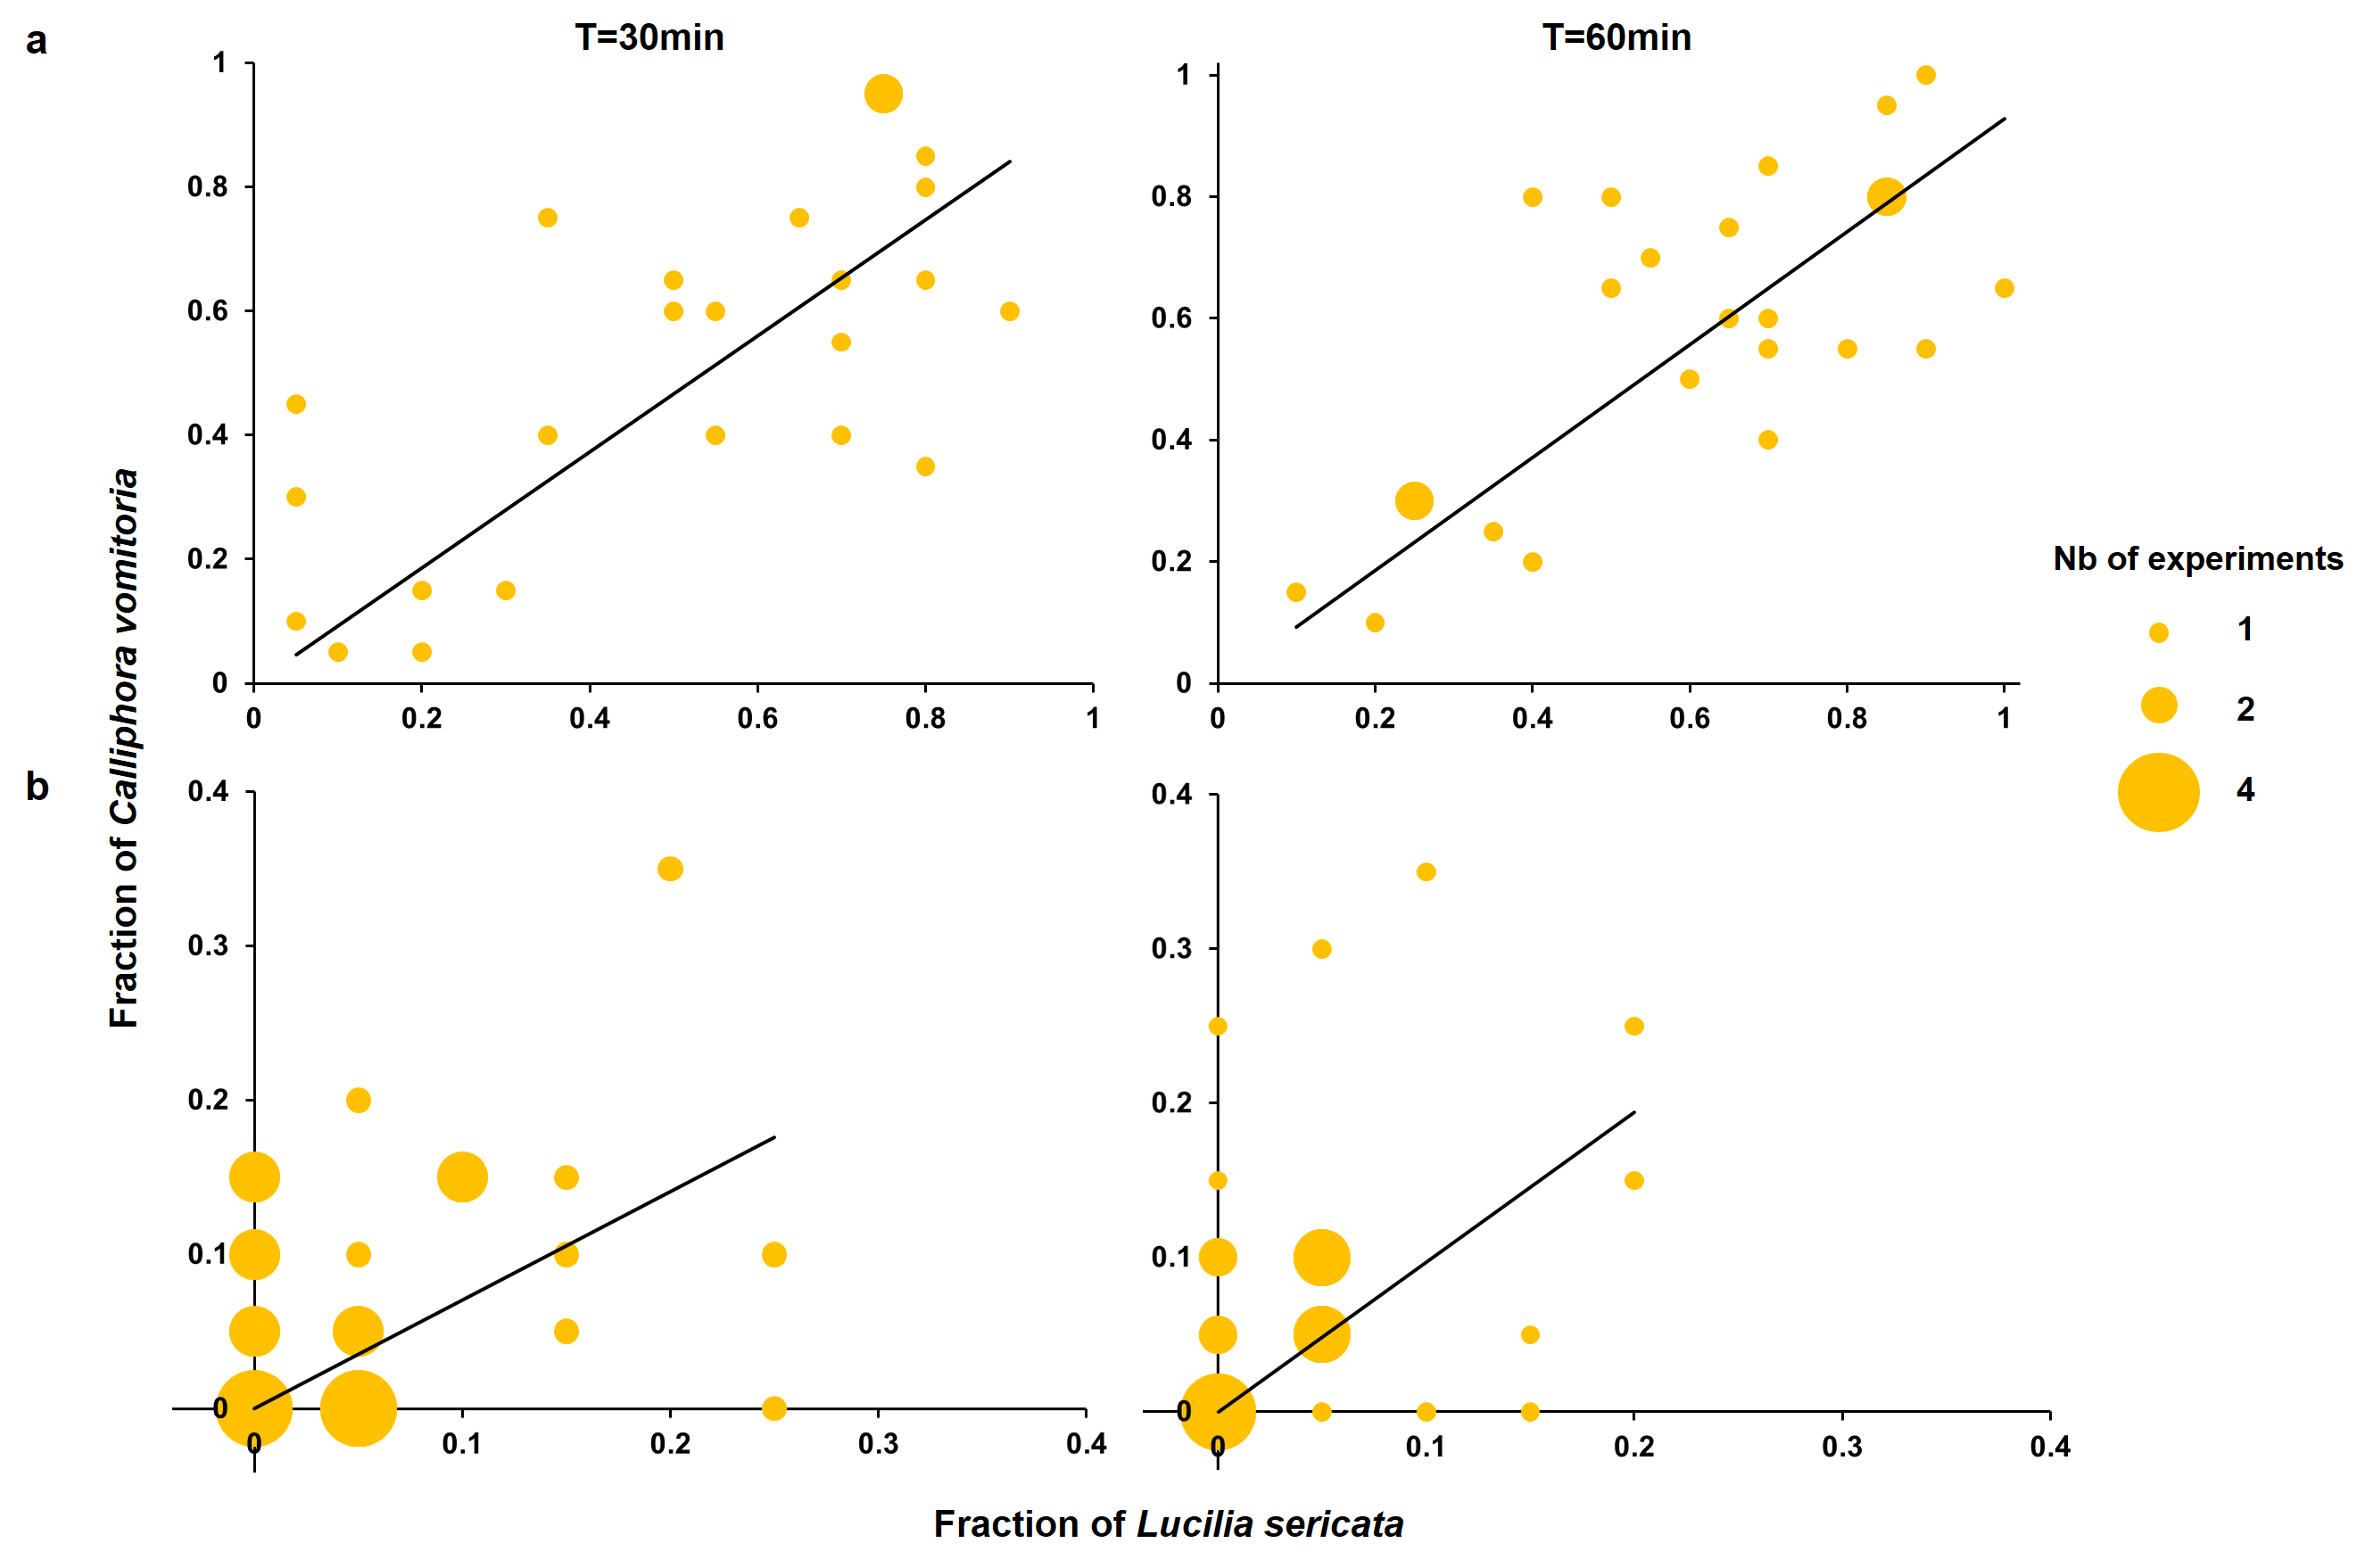
\includegraphics[width=1 \textwidth]{Figures/speciesvsspecies.png}
		\rule{35em}{0.5pt}
		\caption[Species]{\textbf{Repartition of the two studied species in heterospecific groups.} \textbf{a}, Fraction of individuals of each species on the Winner spot during the heterospecific condition experiment (N=24) at t=30 min (linear regression: R\up{2}=0.44; t=12.7, p<0.001) and t=60 min (R\up{2}=0.44; t=15.2, p<0.001). No differences were observed between the mean fractions of \textit{Lucilia sericata} and \textit{Calliphora vomitoria} at t=30 min (W=-26, p>0.5) and at t=60 min (W=50, p>0.1). \textbf{b} Fraction of individuals of each species on the Loser spot during the heterospecific condition experiment (N=24) at t=30 min (linear regression: R\up{2}=-0.1; t=4.3, p<0.001) and t=60 min (R\up{2}=-0.26; t=3.7, p<0.001). No differences were observed between the mean fractions of \textit{L. sericata} and \textit{C. vomitoria} at t=30 min (W=-58, p>0.1) and t=60 min (W=-66, p>0.1).}
	\label{fig:species}
\end{figure}    

\begin{landscape}
\begin{table}[t]
	\caption[Transition]{\textbf{Transitions of tracked individuals between spots during conspecific experiments.} In this study, transition is defined as the duration of time between a zone exit (e.g., Winner spot or Loser spot) and re-entry into that same zone. For both species, the mean number of transitions from Winner to Winner was significantly higher than that obtained for the other transition types (Dunn’s tests, $\alpha$=0.025, p<0.001). For \textit{L. sericata}, no differences were observed in the mean transition times between Winner-to-Winner and Loser-to-Loser transitions (KW= 18.21, p=0.0004; Dunn’s tests, $\alpha$=0.025, p>0.05) and between Winner-to-Loser and Loser-to-Winner transitions (Dunn’s test, $\alpha$=0.025, p>0.05). In contrast, for \textit{C. vomitoria}, the mean transition time for Winner-to-Winner transitions was significantly higher than that for Loser-to-Loser transitions (KW= 24.49, p<0.0001; Dunn’s test, $\alpha$=0.025, p<0.01). No difference was observed between the mean Winner-to-Loser and Loser-to-Winner transition times (Dunn’s test, $\alpha$=0.025, p>0.05).}
    \centering
	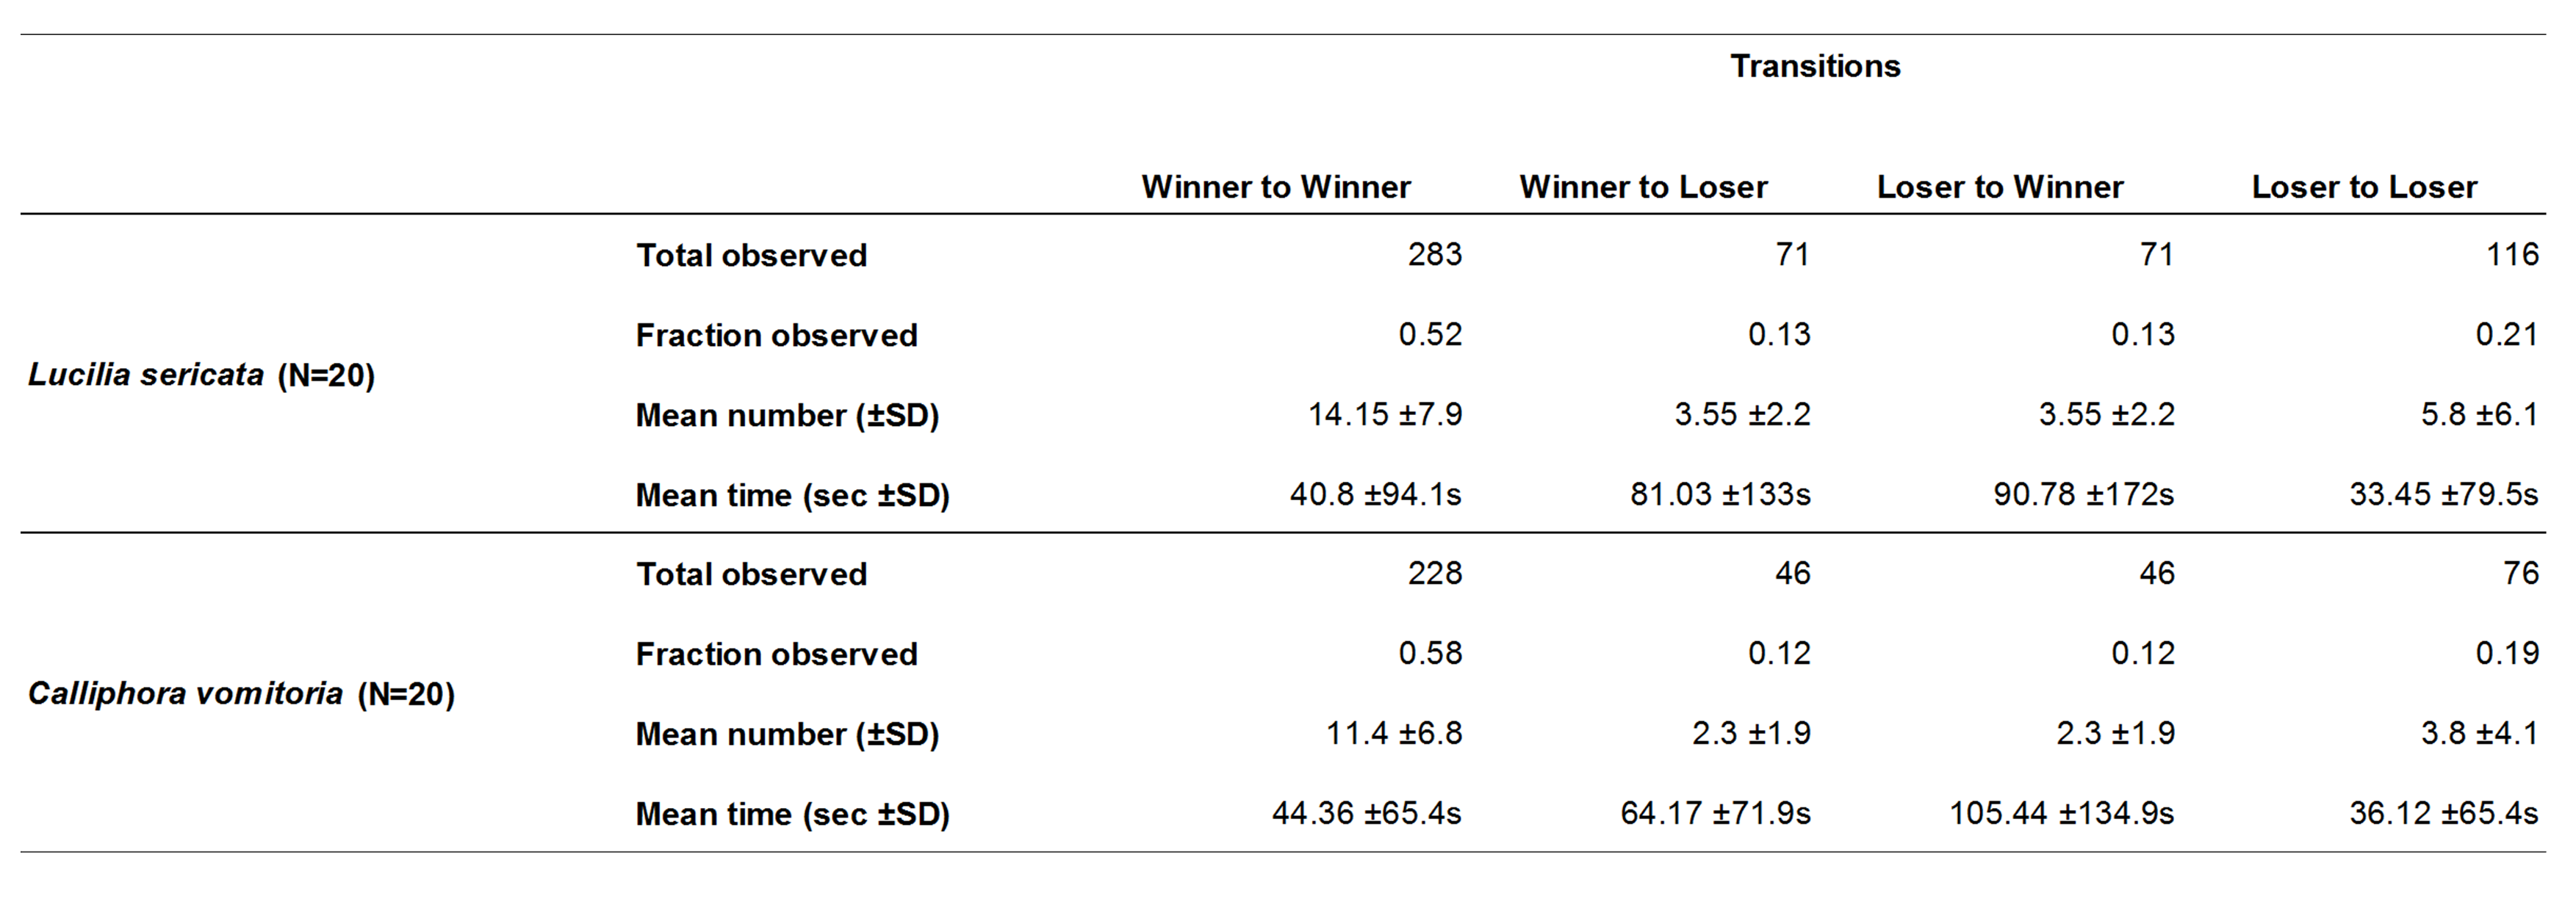
\includegraphics[width=1.5 \textwidth]{Figures/table2.png}
		\label{tab:transition}
\end{table}
\end{landscape}    

\clearpage    
    
    
    
    
    
    
    
    
    
    

% Chapter Template

\chapter{Thermoregulation in gregarious Dipteran larvae: evidence of species-specific temperature selection}

\label{Chapter5}

\lhead{Chapitre 5. \emph{Thermoregulation in gregarious Dipteran larvae: evidence of species-specific temperature selection }} 

Cindy \textsc{Aubernon}\up{a}, Julien \textsc{Boulay}\up{a,b}, Valéry \textsc{Hédouin}\up{a} and Damien \textsc{Charabidzé}\up{a}

\up{a} Univ. Lille, CHU Lille, EA 7367 - UTML - Unité de Taphonomie Médico-Légale, Lille, France\\
\up{b} Université Libre de Bruxelles, Unit of Social Ecology, Brussels, Belgium\\


Article soumis à \emph{Entomologia Experimentalis et Applicata}.

\cleardoublepage
%----------------------------------------------------------------------------------------
%	SECTION 1
%----------------------------------------------------------------------------------------
	\section{Abstract}
There is a clear recognition that local temperature controls the development time of blowfly larvae (Diptera Calliphoridae). In this context, it has been supposed that each species has an optimal development temperature characterized by a short development time and high survival rate. Accordingly, the temperature felt by larvae during their development on a corpse appears to be strongly dependent on behavioural regulation. We hypothesized that the temperature selected by larvae may not only minimize their development time on the cadaver but also may result from a trade-off between development quality and duration. According to this hypothesis, larvae of each species should select the warmest temperature that allows them to develop normally. Consequently, the use of ambient temperature or maximum maggot-mass temperature to estimate the development time of larvae on a corpse would be meaningless.
We designed the Thermograde, which is an 80 cm long linear thermal gradient setup, to determine species-specific preferential temperatures. This experiment was performed using 3 different species: \textit{Lucilia sericata} (Meigen, 1826), \textit{Calliphora vomitoria} (Robineau-Desvoidy, 1830) and \textit{Calliphora vicina} (Linnaeus, 1758). Eighty young third instars were homogeneously placed on the Thermograde along with 500 g of mixed beef liver. The location of larvae in the thermal gradient was observed after 19 h. Fifteen replications were performed for each species. The larvae formed masses that were always located at the same species-specific temperatures, which were 33.3$\pm$1.52\up{o}C for \textit{L. sericata}, 29.61$\pm$1.63\up{o}C for \textit{C. vomitoria} and 22.43$\pm$1.55\up{o}C for \textit{C. vicina}. These innovative results reveal for the first time important information concerning larval displacement and thermoregulation strategies. Our experiments raise questions regarding the way larvae moved on the gradient and located their preferential temperatures. Further studies need to be conducted on individual larva displacement and thermoregulation strategies, which are also important for Post-Mortem Interval (PMI) estimation in forensic entomology. 

\textit{Keywords:} \textit{Calliphora vicina} - \textit{Calliphora vomitoria} - Calliphoridae - collective choice - develoment time - forensic entomology - \textit{Lucilia sericata} - trade-off.

\clearpage

%----------------------------------------------------------------------------------------
%	SECTION 2
%----------------------------------------------------------------------------------------
	\section{Introduction}
Necrophagous blowfly larvae (Diptera Calliphoridae) feed on decomposing remains, mostly on vertebrate cadavers \cite{szpila_key_2009}. Like all poikilothermic species, the internal temperature of larvae depends on the environmental temperature \cite{chapman_insects:_1998}; in other words, their physiological processes are directly controlled by external heat. This is especially true for development speed, which is directly linked to local temperature. Developmental curves generally show a sigmoidal relationship: the development rate is close to zero at low values, increases linearly over a medium range of temperatures, and then slows down at higher temperatures until reaching a lethal point \cite{dent_quantifying_1997}. For necrophagous blowflies, the relationship between temperature and development time has been well-documented in the context of forensic entomology \citep{grassberger_effect_2001,swiger_effects_2007}. Restricting the development-time of necrophagous larvae on the cadaver seems to be essential to prevent food shortages because of the ephemeral duration of animal carcasses in the field \cite{payne_summer_1965}. Furthermore, because the probability of being predated or parasitized increases along with feeding duration on the cadaver, faster development should limit predation or parasitism and increase the larval survival rate \cite{roe_development_2015}. Accordingly, we theorized that larvae would prefer temperatures that speed up their development, thus minimizing the time they must spend on the carcass.  

Various thermoregulation behaviours exist among insects. Because of their poikilothermic physiology, insects select and move between specific micro-climates to adapt their body temperatures \cite{may_insect_1979}. For necrophagous larvae, a preferential choice for warm areas was reported for larvae growing on carcasses that had both sunny and shady sides \cite{sharanowski_insect_2008}. Conversely, larval escape from too-hot locations was also observed \citep{richards_thermal_2009,charabidze_larval-mass_2011}. 

This study was designed 1) to test the ability of necrophagous larvae to orientate in a heterogeneous thermal environment and 2) to compare the temperatures selected by the larvae of 3 common blowfly species. For this purpose, we designed an original setup we named Thermograde. This setup consists of a food-supplied linear thermal gradient that allows larvae to move, feed and grow in close-to-real conditions and to choose to stay and feed at a given temperature (i.e., a location in the Thermograde). Three common species of forensic importance were tested using this setup: \textit{Lucilia sericata} (Meigen, 1826), \textit{Calliphora vicina} (Robineau-Desvoidy, 1830) and \textit{Calliphora vomitoria} (Linnaeus, 1758). 

%----------------------------------------------------------------------------------------
%	SECTION 3
%----------------------------------------------------------------------------------------
	\section{Materials and methods}  
%-----------------------
%	SUBSECTION 1
%----------------------    
    
    	\subsection{Thermograde}
Larvae of three Diptera Calliphoridae species were used in this study; \textit{Lucilia sericata}, \textit{Calliphora vomitoria} and \textit{Calliphora vicina}. The first two strains originated from the north of France, while the \textit{C. vicina} strain originated from Belgium. Insects were reared in tulle cages (50x50x50 cm). Inbreeding was controlled by introducing 50$\%$ wild-type individuals. Adult flies (250$\pm$100) from a single emergence pool were maintained at 20$\pm$2\up{o}C with a daylight photoperiod and for a maximum of 30 days. Flies were fed \textit{ad libitum} with caster sugar and water. To allow egg-laying, 20$\pm$5 g of mixed beef liver was placed in a pill-box inside the insectariums. After egg-laying, the eggs were removed and placed at 19\up{o}C in a climatic chamber (SANYO MIR, 554) in closed plastic boxes (143x105x59 mm) with 100$\pm$5 g of mixed beef liver until reaching the third instar. Corresponding development times for each species at 19\up{o}C were found on the ForenSeek database (https://www.forenseek.org) \citep{greenberg_flies_1991,grassberger_effect_2001,greenberg_different_1993}.

Experiments were performed under controlled conditions using the Thermograde, an apparatus we designed to provide a linear thermal gradient (Figures \ref{fig:thermo1} and \ref{fig:thermo2}). The Thermograde is composed of a heating shelf and a gutter-like galvanized steel bar (5x5x80 cm). Fresh mixed beef liver (500 g) was spread inside the bar to create a 2 cm high food layer. The heating shelf was placed underneath the bar to spread the heat along the bar and obtain a linear thermal gradient inside the beef liver. The shape of this gradient was controlled by changing ambient (i.e., outside the bar) temperature. I-button temperature recorders (DS1921G Thermochron i-Button, $\pm$0.5\up{o}C) were placed every 5 cm (from 2.5 to 77.5 cm) to monitor the local temperature.

For each experiment, 80 young third instars were sampled from the rearing box and starved in a pill-box for 4 hours at 19\up{o}C \cite{charabidze_discontinuous_2013}. This number of insects was previously shown to be sufficient to allow aggregation \cite{boulay_evidence_2013} yet small enough to prevent larval-mass effect and thus heat emission \citep{charabidze_larval-mass_2011,heaton_quantifying_2014}. After starvation, larvae were spread on the beef liver inside the bar in a homogeneous manner (one larva every centimetre). Finally, the bar was closed with an opaque black plastic cap (5.5x3x80 cm).

Experiments were stopped after 19 hours; according to developmental data for the 3 species, this duration was short enough to prevent larvae reaching the wandering stage \citep{greenberg_flies_1991,greenberg_different_1993,grassberger_effect_2001}. The cover was removed, and the Thermograde was divided into 5 cm sections. The beef liver inside each section was removed, and the larvae inside were counted. The temperature values recorded during the experiment were extracted from the temperature recorders. Fifteen replicates were performed for each species.

In addition, 2 control experiments were performed on \textit{L. sericata}. The first control experiment used the Thermograde without heating (Control 1) (i.e., homogeneous temperature, 20$\pm$1\up{o}C) to test the distribution of the larvae inside the Thermograde (6 replications). The second control (Control 2) was designed to ensure that heating had not affected the beef liver’s nutritional value \cite{rice_effects_1953}. Indeed, it can be supposed that larvae might select a given heated area according to the effect of temperature on the nutrient quality of food. For this purpose, 'cooked' liver (37\up{o}C over 19 h) was used instead of fresh beef liver to create the thermal gradient. By doing this, we obtained the same thermal gradient created during the regular (non-control) experiments, but with previously heat-exposed meat. Fifteen replications were performed.

\begin{figure}[ht]
\centering
		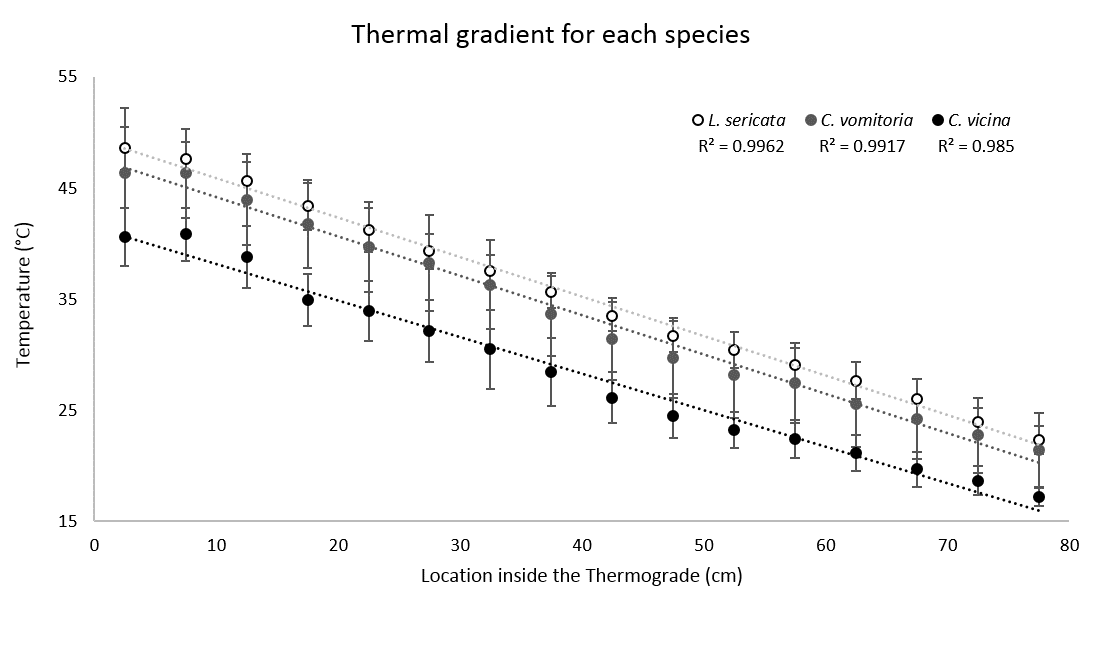
\includegraphics[width=1 \textwidth]{Figures/thermograde1.png}
		\rule{35em}{0.5pt}
		\caption[Thermo1]{The 3 thermal gradients used to test thermal preferences of the species. Points represent the mean temperature ($\pm$SD) inside the food substrate (beef liver) according to their locations inside the Thermograde and the species studied \\(N=15 for each species).}
	\label{fig:thermo1}
\end{figure}

\begin{figure}[ht]
\centering
		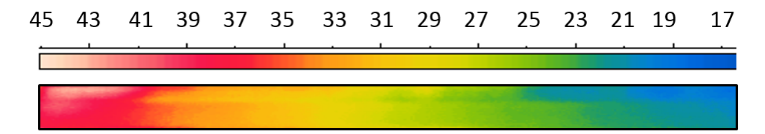
\includegraphics[width=0.9 \textwidth]{Figures/thermograde2.png}
		\rule{35em}{0.5pt}
		\caption[Thermo2]{Thermic photography of the Thermograde for \textit{L. sericata} in Celcius \\degrees (Camera FLIR T425, 320x240 pixels).}
	\label{fig:thermo2}
\end{figure}    
    
%-----------------------
%	SUBSECTION 2
%----------------------    
    
    	\subsection{Binary choice} 
The purpose of this experiment was to test whether the larvae in the Thermograde selected an area based on local temperature or because of food quality resulting from heating. 

The setup was composed of two translucent pill-boxes (150 ml, diam. x h: 57x73 mm) closed with a screw cap drilled with 1 mm holes and connected with a 40 mm long translucent plastic pipe (Figure \ref{fig:setupcindy}). Forty grams of unfrozen beef liver, previously heated for 19 hours at either 33\up{o}C or 37\up{o}C, were placed in each pill-box. The quantity of food in the pill-boxes was selected to expect a 100$\%$ survival rate according to Ireland and Turner \cite{ireland_effects_2006}. Twenty larvae previously starved for 4 h at 19\up{o}C \cite{charabidze_discontinuous_2013} were deposited inside each of these two pill-boxes for a total of 40 larvae per setup. The entire setup was placed in a climatic chamber (SANYO MIR, 554) at 19\up{o}C for 19 h. The pill-boxes and tube were then disassembled, and the larvae inside each of the 3 compartments (the right and left pill-boxes and the tube) were counted. The setup was kept at 19\up{o}C during all experiments, but the liver was heated to varying temperatures before the experiments began. Three liver-temperature conditions were tested: 33\up{o}C vs. 33\up{o}C (i.e., 33\up{o}C control, N=15), 37\up{o}C vs. 37\up{o}C (i.e., 37\up{o}C control, N=15) and 33\up{o}C vs. 37\up{o}C (N=15). 

\begin{figure}[ht]
\centering
		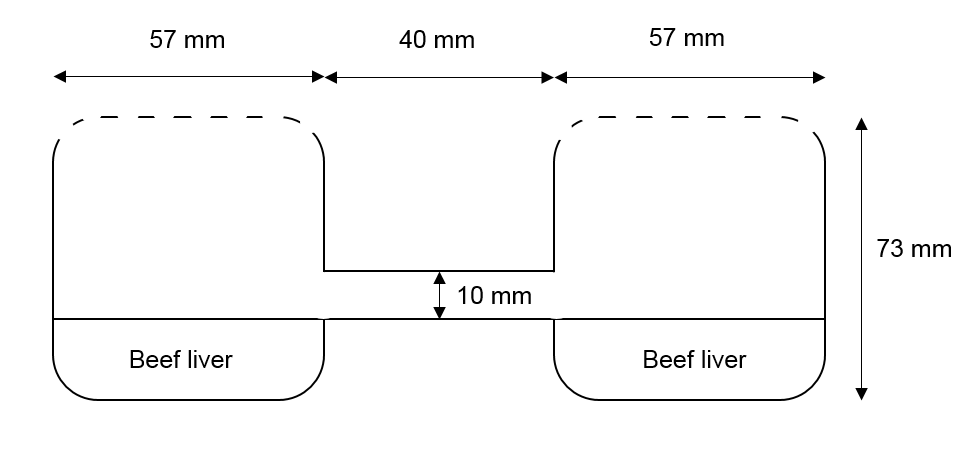
\includegraphics[width=0.9 \textwidth]{Figures/setupbinarycindy.png}
		\rule{35em}{0.5pt}
		\caption[SetupCindy]{Scheme of the binary-choice setup. Beef liver was heated at 33\up{o}C or 37\up{o}C for 19 h before experiments. After the beef liver had cooled to 19\up{o}C, twenty \textit{L. sericata} larvae were placed in each side, and the setup was kept at 19\up{o}C for 19 hours.}
	\label{fig:setupcindy}
\end{figure}    
        
%-----------------------
%	SUBSECTION 3
%----------------------    
    
    	\subsection{Statistical analysis} 
Statistical tests with a significance threshold at 0.05 were used to analyse the results, using XLStat (Addinsoft) software. A chi-square test was used for the larval distribution, and Fisher’s test was used for the distribution of the aggregates. A Shapiro-Wilk’s test and a Bartlett’s test were performed to analyse the mean selected temperature’s distribution and homoscedasticity. An ANOVA and post-hoc Tukey’s and Dunnett’s tests were performed to compare the mean survival rate and the mean selected temperature between species. Finally, a z test was performed to analyse binary choice for each replication, and Student’s t-test was used to compare the mean number of individuals.


%----------------------------------------------------------------------------------------
%	SECTION 4
%----------------------------------------------------------------------------------------
	\section{Results}  
Our setup was designed to allow larval thermal choice under non-stressing rearing conditions. The repartition of \textit{L. sericata} larvae in the Control 1 condition significantly differed from a homogeneous distribution (X\up{2} test: p<0.0001). During each replication, most larvae were observed aggregated together in a single mass. The location of this mass in the setup differed between replicates, but did not statistically differ to a random location (Fisher's test: p=0.82). In other words, without heating (i.e., homogeneous temperature), larvae aggregated together inside the Thermograde, but the location of the aggregate varied between experiments and was not preferentially located in a given area (Figure \ref{fig:percentcindy}). 
When heating was turned on, the thermal gradient inside the Thermograde was close to linear, with a loss of temperature equal to 1.77\up{o}C, 1.77\up{o}C and 1.65\up{o}C per centimeter for, respectively, \textit{L. sericata}, \textit{C. vomitoria} and \textit{C. vicina} (Figure \ref{fig:thermo1}). 

\begin{figure}[ht]
\centering
		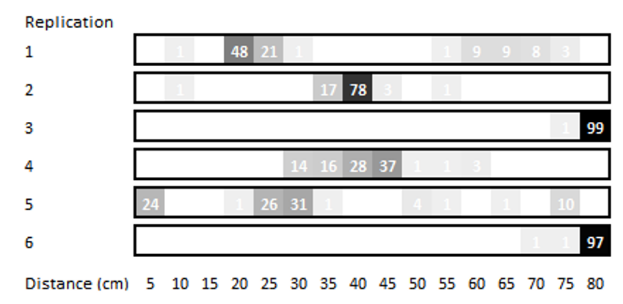
\includegraphics[width=0.9 \textwidth]{Figures/percentcindy.png}
		\rule{35em}{0.5pt}
		\caption[PercentCindy]{Percentage of larvae in each section of the Thermograde according to replication (Control 1). In pale gray, low density of larvae, in dark, high density.}
	\label{fig:percentcindy}
\end{figure}    

Only a few larvae died during experiments. The mean survival rate was 78.42$\pm$14.41$\%$ for \textit{L. sericata}, 87.33$\pm$9.40$\%$ for \textit{C. vomitoria} and 87$\pm$6.57 for \textit{C. vicina}. No difference existed between the survival rates of the tested species and the \textit{L. sericata} survival rate in Control 2 (ANOVA: F=2.12, p=0.11; Tukey’s procedure: \textit{L. sericata} vs. \textit{C. vomitoria}: p=0.16, \textit{L. sericata} vs. \textit{C. vicina}: p=0.14, \textit{C. vomitoria} vs. \textit{C. vicina}: p=1).

The results showed that \textit{L. sericata}, \textit{C. vomitoria} and \textit{C. vicina’s} aggregates (X\up{2} test: p<0.0001) were not randomly located on the thermal gradient (Fisher’s test: \textit{L. sericata}: p=0.01; \textit{C. vomitoria}: p=0.002, \textit{C. vicina}: p<0.0001). Larvae of each species were preferentially observed in a species-specific location corresponding to a given temperature (Figure \ref{fig:boxplotcindy}). \textit{L. sericata} larvae were found located at 33.3$\pm$1.52\up{o}C while \textit{C. vomitoria} larvae were found at 29.61$\pm$1.63\up{o}C and \textit{C. vicina} larvae at 22.58$\pm$1.55\up{o}C. These temperature values differed significantly between the 3 species (ANOVA: F=144.60, p<0.0001; Tukey’s procedure: \textit{L. sericata} vs. \textit{C. vomitoria}: p<0.0001, \textit{L. sericata} vs. \textit{C. vicina}: p<0.0001, \textit{C. vomitoria} vs. \textit{C. vicina}: p=0.0001). 

\begin{figure}[ht]
\centering
		\includegraphics[width=1 \textwidth]{Figures/boxplotcindy.png}
		\rule{35em}{0.5pt}
		\caption[BoxplotCindy]{Box plots representing the location of the larvae according to the temperature gradient inside the Thermograde. The vertical bar inside the box represents the median, the cross represents the mean, and the dots represent outliers, i.e., isolated individuals not located in the aggregate.}
	\label{fig:boxplotcindy}
\end{figure}   

The larval distributions were normal (Shapiro-Wilk’s test: \textit{L. sericata}: W=0.96, p=0.45; \textit{C. vomitoria}: W=0.96, p=0.287; \textit{C. vicina}: W=0.96, p=0.45), and the variance around the mean did not differ according to species (Bartlett’s test: p=0.88) (Figure \ref{fig:districindy}).


\begin{figure}[ht]
\centering
		\includegraphics[width=1 \textwidth]{Figures/districindy.png}
		\rule{35em}{0.5pt}
		\caption[DistriCindy]{Distributions of larvae as density inside the Thermograde for each species according to temperature.}
	\label{fig:districindy}
\end{figure}  



Finally, the repartition of \textit{L. sericata} larvae in Control 2 differed significantly from a homogeneous distribution (X\up{2} test: p<0.0001). Larvae were observed aggregated at a mean temperature of 33$\pm$1.56\up{o}C (Fisher’s test: p=0.01), which was not different from \textit{L. sericata}’s selected temperature during the raw meat experiments (Dunnett’s procedure: p=0.91). Last, we observed a survival rate of 83.25$\pm$6.88$\%$, which was also no different from the raw meat experiments (Dunnett’s procedure: p=0.65). 

Each replicate was divided into one 'winner' pill-box (the one with more larvae inside) and one 'loser' pill-box (Figure \ref{fig:percent2cindy}). We determined the winner and loser pill-boxes according to the number of individuals in each pill-box for each replication by comparing the single proportion with a z test. Three replications (out of 15) were not significant for the 33\up{o}C control, four for the 37\up{o}C control and four 33 vs. 37\up{o}C experiments. These not-significant choices were removed from statistical analysis.

\begin{figure}[ht]
\centering
		\includegraphics[width=1 \textwidth]{Figures/percent2cindy.png}
		\rule{35em}{0.5pt}
		\caption[Percent2Cindy]{Mean percentage of individuals ($\pm$SD) according to experimental conditions. \textbf{A}. Controls (33 vs. 33 and 37 vs. 37) and experiment (33 vs. 37) facing winner (white) and loser (black) pill box.  \textbf{B}. 33 vs. 37\up{o}C.}
	\label{fig:percent2cindy}
\end{figure}  

In the 33\up{o}C control, the 37\up{o}C control and the 33 vs. 37\up{o}C experiments, we noticed that the mean percentage of individuals was higher in winner pill-boxes, with 80.59$\%$ vs. 19.41$\%$ for 33\up{o}C control (Student’s test: p<0.0001), 86.21$\%$ vs. 13.79$\%$ for 37\up{o}C control (Student’s test: p<0.0001) and 83.58$\%$ vs. 16.42$\%$ for 33 vs. 37\up{o}C experiment. Finally, we noticed that for the 33 vs. 37\up{o}C experiment, the 33\up{o}C pill-box won 49.12$\%$ of the time, while the 37\up{o}C pill-box won 50.88$\%$ of the time — that is, 33\up{o}C was the winner 5 times and 37\up{o}C was the winner 6 times. This did not differ from an equal (fifty-fifty) repartition (z test: p=0.76; X\up{2} test: p=0.90). Last, the mean percentage of individuals was the same in both 33\up{o}C and 37\up{o}C pill-boxes (Student’s test: p=0.939) and did not show larval preference for a given food substrate.
        
  
%----------------------------------------------------------------------------------------
%	SECTION 5
%----------------------------------------------------------------------------------------
	\section{Discussion}    
  
This study is the first observation of collective preferential temperature selection by 3 species of necrophagous larvae of forensic importance. The highlight of this study was that the larvae of each species were able to locate and select a preferred species-specific temperature. These values were 33.3$\pm$1.52\up{o}C for \textit{L. sericata}, 29.6$\pm$1.63\up{o}C for \textit{C. vomitoria} and 22.43$\pm$1.55\up{o}C for \textit{C. vicina}. Such a clear result raises interesting questions regarding developmental physiology and trade-off selection in necrophagous larvae.

It is known from the literature that a measurable increase in temperature can arise inside aggregates (larval-mass effect) \citep{slone_thermoregulation_2007,charabidze_larval-mass_2011}. Such local heating begins with an aggregate of approximately 1000 third instar individuals and increases with the quantity of larvae \cite{heaton_quantifying_2014}. During our experiments, the number of larvae was kept low enough to prevent this phenomenon, and thermometers inside the bar did not record any local increase of temperature in the places where larvae were aggregated. Accordingly, any maggot-mass effect in our experiment can be excluded. One might also object that the larvae did not select a given temperature but instead selected a food quality. According to this view, the nutritional value of the beef liver should change depending on its temperature and according to species. However, considering \textit{L. sericata}, no preference was observed between experiments with raw or 37\up{o}C-incubated food (Control 2). Furthermore, binary-choice test experiments did not show any larval preference between 33\up{o}C- or 37\up{o}C-incubated food; larvae were gathered at both temperatures and at the same mean percentage. We concluded from these experiments that larval distribution in the Thermograde was due not to differences in food quality, but to preferential temperature selection.

Larvae were able to aggregate and gather themselves into a single group inside the Thermograde \citep{rivers_physiological_2011,boulay_evidence_2013}. Under Control 1’s conditions (20$\pm$1\up{o}C homogeneous temperature, no heating), these aggregates were located randomly throughout the apparatus. This control demonstrates that the distributions observed in the gradient experiments were not due to setup bias or increased probability to cross and aggregate in the middle of the Thermograde. On the contrary, for the 3 tested species, aggregates clearly occurred in different areas of the Thermograde at given species-specific temperature values. In addition to the well-known larval aggregation behaviour \cite{boulay_evidence_2013}, our results demonstrate for the first time the search and collective choice behaviour of necrophagous larvae for a given temperature. A key point is that this temperature differed between the three studied species; the selected temperature was highly species-specific. Indeed, while \textit{L. sericata} larvae were always found strongly grouped at approximately 33.3$\pm$1.52\up{o}C, \textit{C. vomitoria} larvae aggregated in the 29.61$\pm$1.63\up{o}C part of the Thermograde, and \textit{C. vicina} larvae were found located at 22.43$\pm$1.55\up{o}C.
        
In a recent study, \citet{johnson_tracking_2014} studied larval temperature selection of two necrophagous species, \textit{C. vicina} and \textit{Chrysomya rufifacies} (Macquart, 1842). Using a thermal gradient created with a heating spot and a cold bath, the authors observed three times the selection of third instar larvae placed in the setup. The larval-selected temperature was defined as the value where larvae stopped and stayed after 2 hours; the temperature at this point was then measured. According to this protocol, \citet{johnson_tracking_2014} observed that \textit{C. vicina} larvae selected 'temperature approximately 24.5\up{o}C'. This value is 2\up{o}C above the one we measured (22.43\up{o}C). This difference may be explained by the few replicates performed (only 3 with 3\up{rd} instar), the exactness of the thermal gradient used (the temperature was known each 10 cm in a range of 23\up{o}C to 54\up{o}C) or by differences between the two studied insect populations. Indeed, the \textit{Calliphora vicina} larvae studied by \citet{johnson_tracking_2014} came from Australia, while those used for this study came from Belgium. It is known from the literature that local fly populations are morphologically and physiologically adapted to their environment \citep{donovan_larval_2006,lebouvier_significance_2011,tarone_population_2011}. For example, differences exist in the diapause and low-temperature survival rates between Scottish, Finnish and Italian populations of \textit{C. vicina} \cite{saunders_effects_2013}. \textit{C. vicina} from Switzerland have even been shown to develop in extremely cold environments that are usually not suitable for this species \cite{faucherre_behavior_1999}.     

The reasons behind the temperature choices by each species are still unknown. Larvae feeding and growing on carrion face high selection pressure \cite{campobasso_factors_2001}. This is noticeably true during feeding stages; decomposition processes can alter flesh within a few days, and quick drying of the tissues can make cadavers inedible for blowfly larvae \cite{clark_postmortem_1997}. Last but not least, numerous opportunistic scavengers, such as wild boars, foxes or crows, can eat small cadavers or deflesh larger ones in a few minutes \cite{haglund_dog_1997}. Bearing this in mind, it appears that larvae should tend to minimize their development duration and thus the time spent on the cadaver. This can be achieved by individuals moving to high-temperature areas and thus increasing their development rate \cite{grassberger_effect_2001}. According to this assumption, larvae of each species should select the warmest temperature allowing their development. However, developmental data currently available from the literature do not validate this hypothesis. Indeed, published developmental data are mostly restricted to low- or medium-temperature ranges; only a few values are available for high temperature. \citet{reiter_growth_1984} noticed that when constant temperatures were beyond 30\up{o}C, \textit{C. vicina} larvae were deformed and or died. \citet{donovan_larval_2006} reported a larval lethal temperature for \textit{C. vicina} of 35\up{o}C, more than 10\up{o}C above the value larvae selected in the Thermograde. However, we hypothesized that the temperature preferred by larvae would not be selected solely to minimize development time on the cadaver, but instead may result from a trade-off between development quality and duration. Indeed, temperature controls not only the physiology of the larvae and their development rate \cite{chapman_insects:_1998} but also the quality of their growth and thus their fitness. Larvae growing under too-warm temperatures could be malformed or too small \cite{reiter_growth_1984}, and physiological parameters, such as respiration or eggs, may also be impacted \cite{williams_growth_1984}. Such effects are even transmitted to the second generation: \citet{zamudio_bigger_1995} demonstrated that \textit{Drosophila melanogaster} (Meigen, 1830) fitness depends on parental rearing temperature. Detailed developmental data (duration, survival rate, length and weight) at high temperature would thus be necessary to verify our developmental trade-off hypothesis; breeding experiments are currently being performed in our laboratory to gather developmental data at high temperature for the 3 species targeted by this study.

Finally, our experiments raise questions regarding the way larvae moved on the gradient and located their preferential temperature. From our results, it is not possible to determine whether the aggregate was created by the sum of individual thermal preferences, or whether larvae first aggregate and then move together. Previous studies of maggot masses noticed a turnover of larvae inside masses, a behaviour that supposedly allows larvae cooling and prevents overheating of the aggregates \citep{charabidze_discontinuous_2013,rivers_heat_2015}. Further studies need to be conducted on individual larvae displacement and thermoregulation strategies, which are also important for post-mortem interval (PMI) estimation in forensic entomology. 

%----------------------------------------------------------------------------------------
%	SECTION 6
%----------------------------------------------------------------------------------------
	\section{Acknowledgments}   
Authors would like to thanks Luc Bourguignon and Yves Braet for providing \textit{Calliphora vicina} strains.     
        
        
\clearpage    
    
    
% Chapter Template
\setcounter{chapter}{6}
\chapter*{Discussion et conclusion} % Main chapter title
\addcontentsline{toc}{chapter}{Discussion et conclusion}
\label{Discussion} % Change X to a consecutive number; for referencing this chapter elsewhere, use \ref{ChapterX}

\lhead{\emph{Discussion et conclusion}} % Change X to a consecutive number; this is for the header on each page - perhaps a shortened title

\textit{``L'égalité, la seule égalité en ce monde, l'égalité devant l'asticot."}

\begin{flushright}
Jean-Henri Fabre (1823-1915)
\end{flushright}

\cleardoublepage

%----------------------------------------------------------------------------------------
%	SECTION 1
%----------------------------------------------------------------------------------------
    
	\section{Les larves nécrophages: un nouveau modèle d'étude}  
    
Les larves nécrophages de Diptères étaient jusqu'à présent étudiées principalement en entomologie forensique, un cadre scientifique à visée applicative immédiate. En effet, ces insectes sont d'importance en entomologie forensique car ils arrivent très tôt sur un cadavre et sont donc utilisés par les experts pour effectuer une datation du décès (calcul de l'Intervalle Post-Mortem minimum (IPMmin); cf. Introduction \ref{subsubsec:forensique}). Des études physiologiques sur le développement des larves ont été nécessaires pour affiner ces techniques de datation. Ces études ont permis, entre autres, de connaître les durées de développement en fonction de la température \cite{grassberger_effect_2001}, l'impact de la qualité nutritive d'une ressource sur les larves \cite{ireland_effects_2006} ou encore les effets des produits chimiques sur leur développement \cite{aubernon_experimental_2015}. La physiologie des larves est donc bien connue, mais leur comportement reste encore peu étudié, comme le souligne \citet{rivers_physiological_2011} dans leur revue.

Notre approche éthologique amène une vision nouvelle de la vie de ces insectes, et  aborde notamment des questions fondamentales. L'étude des comportements collectifs des larves nécrophages s'ajoute à celle faite sur d'autres espèces sociales comme les blattes \cite{canonge_individuel_2011}, les fourmis \cite{dussutour_organisation_2004}, les poissons \cite{robert_does_2013} ou encore les oiseaux \cite{farine_collective_2014}. Les larves nécrophages sont un modèle biologique inédit offrant des perspectives intéressantes dans ce cadre d'étude. En effet, l'observation quasi systématique de groupes hétérospécifiques et la capacité des larves à modifier leur environnement de manière significative permettent l'étude de plusieurs phénomènes comportementaux et évolutifs. Parmi ces phénomènes, on peut notamment citer les phénomènes de coopération-compétition qui peuvent exister entre deux espèces appartenant à un même groupe social (cf. Chapitre \ref{Chapter1}).     



%----------------------------------------------------------------------------------------
%	SECTION 2
%----------------------------------------------------------------------------------------     
		\section{L'individu}     
Nos études réalisées sur le comportement individuel offrent un aperçu des mécanismes qui sous-tendent la formation et le maintien des groupes de larves. L'un de ces mécanismes étant le signal déposé au sol passivement par les larves et reconnu par les congénères. Ce type de marquage chimique tactile a été décrit chez plusieurs espèces d'insectes comme les fourmis \cite{devigne_how_2006} ou encore les coccinelles \cite{durieux_role_2012}. Les molécules responsables de cette reconnaissance sont généralement des hydrocarbures cuticulaires. 

			\subsection{Attraction/rétention du signal larvaire}
Nos tests de choix binaire ont mis en évidence le dépôt au sol passif d'un composé chimique (cf. Chapitre \ref{Chapter2}). Ce dépôt a un effet d'attraction et de rétention sur les congénères \cite{boulay_evidence_2013}. De plus, les larves sont capables, via le scanning, de détecter ce signal et de le suivre (cf. Chapitre \ref{Chapter3}). Ces observations suggèrent que ce signal larvaire serait impliqué dans l'agrégation de ces espèces. Cette attraction à très courte distance nécessite d'être testée à plus grande distance à l'aide d'olfactomètres, comme ce qui a été fait chez le lombric \cite{zirbes_earthworms_2011}. \citet{zirbes_earthworms_2011} ont observé une capacité des lombrics à détecter à distance et à rejoindre les signaux volatils émis par des congénères.

Des tests complémentaires de choix binaires (cf. Annexe \ref{Annexes1}, expérience 2 du Chapitre \ref{Chapter2}) ont montré que des larves de \textit{Calliphora vomitoria} passent significativement plus du temps dans une zone où 10 larves de \textit{Lucilia sericata} avaient été laissées pendant 10min (comparativement à une zone vierge de dépôt). Ce résultat suggère une reconnaissance interspécifique du signal ainsi que la conservation de son effet attractif/rétentif chez une espèce proche. Une telle reconnaissance est nécessaire pour l'établissement et le maintien des groupes contenant plusieurs espèces (cf. Chapitre \ref{Chapter1}). La proximité anatomique des organes  sensorielles des larves entre les espèces (cf. Introduction \ref{subsubsec:anatomie}, \citep{chu-wang_fine_1971}) et l'observation d'un même comportement exploratoire caractéristique (scanning) laissent à penser que la reconnaissance du signal larvaire seraient sous tendue par les mêmes mécanismes physiologiques et comportementaux, favorisant ainsi l'existence de vecteurs d'agrégation interspécifiques.


			\subsection{Identification du marquage chimique}
Une première analyse chromatographique du signal larvaire a été entreprise chez \textit{Lucilia sericata} avec l'équipe du Pr. Georges \textsc{Lognay} (Départ. Chimie Analytique, Agro-Bio-Tech Gembloux). Les résultats ont montré une composition largement dominée par le cholestérol (Cholest-5-en-3-ol(3$\beta$); cf. Annexe \ref{Annexes1}). Les tests comportementaux préliminaires n'ont pas mis en évidence d'attraction/rétention significative des larves pour ce composé (protocole basé sur l'expérience 2 du Chapitre \ref{Chapter2}). Des tests plus approfondis seraient nécessaires pour identifier précisément chaque composé chimique et les tester sur les individus. Des études d'identification des hydrocarbures cuticulaires ont déjà été réalisées chez les larves nécrophages de Diptères \citep{roux_ontogenetic_2008,zhu_development_2006}, mais, à l'heure actuelle, la composition chimique du dépôt laissé par les individus n'est pas connue.

Dans un premier temps les composés lourds seraient identifiés via une chromatographie en phase gazeuse. Puis dans une seconde étape, les composés volatils seraient analysés suivant le protocole de \citet{frederickx_volatile_2012}. En effet, si l'effet rétentif du signal est vraisemblablement porté par des molécules lourdes (i.e. longues chaînes carbonnées qui restent au sol), nous pouvons penser que l'effet attractif serait supporté par les molécules volatiles. Des tests comportementaux d'attraction et de rétention avec les composés identifiés permettraient ainsi de mettre en évidence les molécules impliquées.

D'après nos observations en individuel et en collectif d'une reconnaissance interspécifique des vecteurs d'agrégation (cf. Chapitre \ref{Chapter4}), une analyse comparative des profils chromatographiques des signaux déposés par \textit{L. sericata} et \textit{C. vomitoria} est une approche à privilégier. En effet, elle permettrait d'identifier les composés en communs et de les tester en priorité sur les individus des deux espèces dans des tests de choix.
            

%----------------------------------------------------------------------------------------
%	SECTION 3
%----------------------------------------------------------------------------------------       

		\section{Le groupe}
Le comportement d'agrégation des larves semble être une réponse adaptative efficace face aux contraintes liées à cet environnement particulier qu'est le cadavre. En effet, un cadavre est un milieu instable, à haute valeur nutritionnelle donc compétitif mais éphémère. A l'heure actuelle, deux bénéfices de l'agrégation sont bien connus et étudiés dans la littérature : la génération de chaleur \citep{slone_thermoregulation_2007,charabidze_larval-mass_2011} et la production accrue par le nombre de liquides d'excrétion/sécrétion riches en enzymes et en antibiotiques \citep{wilson_impacts_2015,sandeman_tryptic_1990}. \citet{rivers_physiological_2011} avancent d'autres bénéfices liés à l'agrégation, notamment une protection contre les prédateurs, une limitation de la dessiccation et une meilleure assimilation de la nourriture. Bien que ces avantages soient, au regard d'autres études sur les agrégations d'arthropodes \cite{jeanson_key_2012}, intuitifs, ils n'ont pas été mis en évidence expérimentalement. Tout comme ces bénéfices, les mécanismes qui sous-tendent la stabilisation des masses larvaires sont méconnus et peu étudiés.

Nous avons vu que le comportement d'agrégation des larves est très marqué et que la formation des groupes est rapide (cf. Chapitres \ref{Chapter2} et \ref{Chapter4}). Nos résultats ont démontré que l'agrégation des larves était active et n'était pas seulement la résultante de l'agrégation des pontes par les femelles \cite{fenton_oviposition_1999}. Dans nos expériences, un comportement de thigmotactisme positif a été observé (cf. Chapitre \ref{Chapter2}), comportement également présent chez d'autres espèces d'arthropodes (e.g. cloportes \cite{devigne_individual_2011} ou acariens \cite{mailleux_collective_2011}). Ce comportement peut expliquer la localisation proche des parois de l'arène de l'agrégat observé en début d'expérience (cf. Chapitre \ref{Chapter2}). En revanche, après 24h, l'agrégat s'était déplacé, suggérant un thigmotactisme interindividuel plus important dû fait d'un nombre d'individus accru présents au sein du groupe. Ce mouvement régit par le contact entre individus est également observé chez les criquets grégaires \cite{simpson_gregarious_2001}. Ces insectes forment d'immenses agrégats pouvant contenir des milliers d'individus ravageant les cultures \citep{buhl_using_2012,buhl_group_2010}. Ces bancs de criquets peuvent prendre différent patterns : l'espèce \textit{Chortoicetes terminifera} (présente en Australie) forme un groupe avec un front dense alors que l'espèce \textit{Locustana pardalina} (présente dans le sud de l'Afrique) est observée en bancs formés par des colonnes d'individus. Les mécanismes aboutissant à ces patterns restent méconnus (e.g. impact de la végétation, comportement individuel) mais la démarche de ces auteurs alliant modélisation mathématique et observations en laboratoire/terrain est intéressante. Cette démarche offre une piste de recherche supplémentaire pour l'étude du comportement d'agrégation des larves nécrophages.

		\subsection{Dynamique d'agrégation}
Les dynamiques de choix observées avec des groupes monospécifiques (cf. Chapitre \ref{Chapter4}) sont comparables à celles retrouvées chez les blattes \citep{canonge_self-amplification_2009,jeanson_self-organized_2005} ou les cloportes \cite{devigne_individual_2011}. Un choix clair pour un site d'agrégation est fait en quelques minutes par les larves (en moins de 5min, 50$\%$ des individus ont sélectionné un spot) et ce choix est maintenu dans le temps. Cette prise de décision collective peut être définie comme étant une décision consensuelle selon \citet{conradt_consensus_2005}. En effet, aucun conflit intérêt\footnotemark[1]\footnotetext[1]{\textit{Conflit d'intérêt}: apparaît quand un individu ou une organisation est impliquée dans de multiples intérêts, l'un d'eux pouvant corrompre la motivation à agir sur les autres} n'est observé et au vu des organes sensoriels des larves et de leur sensitivité (cf. Introduction \ref{subsubsec:anatomie}), une communication au niveau local\footnotemark[2]\footnotetext[2]{\textit{Communication locale}: les membres d'un groupe ne peuvent communiquer qu'avec leur plus proche voisin \cite{conradt_consensus_2005}.} est à privilégier. Ces caractéristiques aboutissent, selon \citet{conradt_consensus_2005}, à une décision collective classée de consensuelle. Les mécanismes régissant ce type de décision sont ceux de l'auto-organisation (cf. Introduction \ref{sec:autoorganisation}). Des études comportementales restent cependant à réaliser pour étayer l'idée d'un système auto-organisé. Par exemple, l'existence d'un éventuel quorum\footnotemark[3]\footnotetext[3]{\textit{Quorum}: nombre minimum d'individus nécessaire pour prendre ou favoriser une action particulière influençant l'ensemble du groupe à adopter cette action.} pourrait être analysée en faisant varier le nombre d'individus placés dans l'arène (e.g. 10, 20 ou 30 individus). Les études sur les blattes sont un bon exemple de ce phénomène et un modèle de comparaison intéressant \citep{sempo_complex_2009,jeanson_self-organized_2005}.

Notre travail a mis en évidence la dynamique d'agrégation d'un groupe composé de deux espèces (cf. Chapitre \ref{Chapter4}). Un choix collectif pour un site est observé, mais ce choix se fait plus lentement qu'avec un groupe composé par une seule espèce (cf. Chapitre \ref{Chapter4}). Ces observations laissent sous entendre que les deux espèces de larves partagent les mêmes mécanismes d'agrégation, ou du moins une partie. Une reconnaissance interspécifique du signal déposé par les larves est notamment suggérée  (cf. Chapitre \ref{Chapter2}). Cette reconnaissance interspécifique serait moins efficace qu'une reconnaissance intraspécifique, créant une dynamique d'agrégation du groupe plus lente (comme observée). Cela laisse également à penser que ces 2 espèces pourraient, en conditions naturelles, coopérer pour aboutir à des tailles de groupe suffisamment importante, probablement dans le but ultime d'obtenir les bénéfices liés à l'agrégation (effet Allee). Des études similaires réalisées en faisant varier la quantité de ressources et le nombre d'individus de chaque espèce permettraient d'étudier une éventuelle limite entre coopération et compétition. De plus, ce type d'études offrirait une vision des phénomènes d'exclusion/ségrégation entre les espèces observées dans la nature (cf. Chapitre \ref{Chapter1}). 

Une telle ségrégation peut être impactée par la température locale. Nous avons observé que chaque espèce avait un préférendum thermique (cf. Chapitre \ref{Chapter5}). Comme prochaine étape, il serait intéressant d'observer deux populations de larves d'espèces différentes placées sur le gradient thermique utilisé dans l'étude du Chapitre \ref{Chapter5} (Thermograde). Ce type d'expérience, actuellement en cours au laboratoire (thèse de C. \textsc{Aubernon}), permettra d'étudier la place du comportement social face aux préférences thermiques des larves. Est-ce qu'une ségrégation du groupe va être observée avec chaque espèce présente au niveau de sa température préférentielle ? Ou à l'inverse un groupe mixte formé à une température intermédiaire ? Si une ségrégation est observée, la recherche d'une température préférée passerait en priorité sur la formation d'un groupe mixte. La température serait un vecteur d'agrégation lié à l'espèce. \textit{A contrario}, si un groupe interspécifique est formé cela supposerait que les larves cherchent dans un premier temps à s'agréger avec des congénères même si la température recherchée est à proximité. Cette dernière observation supposerait que les vecteurs d'agrégations interspécifiques, autre que la chaleur, seraient prédominants sur la température. Ce compromis entre agrégation et température est une piste de recherche intéressante et novatrice qui permettra de mieux comprendre les avantages recherchés par les larves.

		\subsection{Attraction/rétention du groupe}
Les phénomènes d'attraction/rétention que peut avoir un groupe sur un individu sont à la base de l'émergence des systèmes complexes. Ils sont observés chez les blattes \citep{canonge_individuel_2011,lihoreau_collective_2010}, les cloportes \cite{devigne_individual_2011} ou encore les chenilles \cite{fitzgerald_specificity_1979}. Ces phénomènes conduisent à des amplifications du système (cf. Introduction \ref{sec:amplification}), ces mécanismes étant liés aux structures auto-organisées. 

L'effet attractif permet à la larve de localiser, plus ou moins à distance, le groupe. Dans notre système larves/sites de nourriture (cf. Chapitre \ref{Chapter4}), le suivi d'un individu met en évidence à la fois une attraction et une rétention du groupe. Des tests préliminaires ont montré qu'une larve de \textit{Lucilia sericata} était également attirée par un groupe de congénères présent à distance. Dans un olfactomètre à deux branches avec pour choix un groupe de 40 individus et un témoin (vide), les larves ont choisi dans 100$\%$ des essais la branche contenant le groupe (cf. Annexe \ref{Annexes1}). Ce résultat préliminaire sous-tend une attraction à distance du groupe sur l'individu. Ce type d'effet a été mis en évidence chez les groupes de blattes \cite{ame_cockroach_2004} ou encore les lombrics \cite{zirbes_earthworms_2011}.

L'effet rétentif va maintenir la cohésion sociale entre les membres du groupe. Basés sur le modèle blatte \cite{canonge_individuel_2011}, des tests comportementaux où la taille du groupe va varier vont nous permettre de complémenter notre observation d'un tel effet chez les groupes de larves (cf. Chapitre \ref{Chapter4}). Associés à l'effet attractif du groupe (recherche de congénères), ces effets rétentifs amplifient le système et aboutissent à la formation des structures auto-organisées. Il convient, cependant, de garder à l'esprit que des phénomènes d'encombrement peuvent être observés au sein des agrégats, se traduisant par une bousculade permanente pour l'accès à la nourriture (\textit{scramble competition} \cite{rivers_physiological_2011}).

%----------------------------------------------------------------------------------------
%	SECTION 4
%----------------------------------------------------------------------------------------       
		\section{La modélisation comme prochaine étape}  
        
Notre étude est la première étape vers une compréhension plus globale des groupes interspécifiques. En effet, dans leur ouvrage de référence, \citet{camazine_self-organization_2001} proposent une méthodologie à adopter lors de l'étude des comportements collectifs (appelée \textit{bottom-up}; Figure \ref{fig:model}). Ils présentent 4 étapes : (i) la description du phénomène collectif et notamment sa dynamique, (ii) l'identification des comportements individuels et des interactions interindividuelles qui permettent d'expliquer la dynamique collective, (iii) la formulation d'un modèle sur la base des règles comportementales caractérisées précédemment, et enfin (iv) la comparaison entre la dynamique collective obtenue avec le modèle et celle acquise expérimentalement. Cette démarche montre bien le va-et-vient nécessaire entre les observations expérimentales et la modélisation mathématique. Ce cycle de travail amène à une meilleure compréhension du système collectif étudié.

La modélisation mathématique a ceci d'avantageux qu'elle permet de caractériser l'organisation et la structure d'un groupe composé d'une multitude d'individus avec un nombre d'événements (e.g. interactions sociales) important. Elle offre plusieurs avantages à l'utilisateur une fois celle-ci fidèle aux observations expérimentales. Elle permet d'avoir un nombre de réplications bien plus important qu'en conditions expérimentales et de faire varier les paramètres aisément (e.g. taille du groupe ou nombre d'abris). Outre ces avantages, la modélisation mathématique, couplée à la simulation, permet de déterminer les vecteurs nécessaires et suffisants pour produire les phénomènes observés. Cette démarche simplifie la compréhension des systèmes complexes. Des premières réflexions sur cette étape ont été entamées avec G. \textsc{Sempo} et A. \textsc{Campo} (Unité d'Écologie Sociale, ULB), et offriront une base de travail pour une étude de modélisation.

\begin{figure}[ht]
	\centering
		\includegraphics[width=0.8 \textwidth]{Figures/modelisation.png}
		\rule{35em}{0.5pt}
	\caption[Model]{Schéma présentant les différentes étapes lors de l'étude des comportements collectifs (tiré de \citet{camazine_self-organization_2001}).}
	\label{fig:model}
\end{figure}


%----------------------------------------------------------------------------------------
%	SECTION 5
%----------------------------------------------------------------------------------------     
    \section{Perspectives en entomologie forensique}
    
Ce travail de thèse a mis en évidence l'aspect fondamental de la vie sociale chez les larves nécrophages de Diptères, des espèces d'importance en entomologie forensique. Ces groupes sociaux impactent de manière significative le développement des larves. Lors d'une expertise judiciaire, il est primordial pour l'expert entomologiste de connaître les conditions dans lesquelles se sont développées les insectes retrouvés sur un corps (e.g. température, présence de substances toxiques, etc.). Ces conditions de vie vont directement affecter les durées de développement des insectes et donc la datation du décès. A l'heure actuelle, l'impact des conditions locales et du comportement larvaire ne sont que trop rarement pris en compte.

Il est facile d'imaginer qu'une larve de Diptères prélevée sur un cadavre au sein d'un groupe de quelques individus n'aura pas eu accès aux mêmes bénéfices liés au groupe qu'une larve extraite au milieu de milliers. Cette dernière aura bénéficié, entre autres, du dégagement de chaleur (i.e. génération significative observée avec des groupes au-delà de 1000 individus \cite{johnson_effect_2014}) accélérant son développement. Il est donc nécessaire de mettre en place des outils, qualitatifs dans un premier temps, permettant d'intégrer la variabilité due au comportement social des larves nécrophages lors d'une découverte de cadavre. Une fois nos connaissances approfondies sur l'impact de la taille du groupe sur le développement des larves, des outils quantitatifs viendront s'ajouter. Ces outils permettront, \textit{in fine}, d'affiner les techniques actuelles de datation entomologique du décès en tenant compte du comportement social des larves nécrophages.


%----------------------------------------------------------------------------------------
%	SECTION 6
%----------------------------------------------------------------------------------------         
    \section{Conclusion}    
    
Pour conclure, ce travail a mis en évidence les dynamiques de formation des groupes et les mécanismes qui sous-tendent ces regroupements des larves nécrophages de Diptères. Ce grégarisme impacte de manière significative la vie de ces insectes. La démarche expérimentale de va-et-vient entre le comportement individuel et collectif des larves adoptée dans ce travail ouvre à des études éthologiques et de modélisation futures. 

Un agrégat de plusieurs milliers de larves sur un cadavre peut être vu comme un \textit{immense estomac} (une idée avancée par D. \textsc{Charabidzé}). En effet, un groupe de larves nécrophages va produire des enzymes \cite{wilson_impacts_2015}, générer de la chaleur \cite{charabidze_larval-mass_2011}, modifier localement le pH et les populations bactériennes, et avoir une action mécanique. Ces différents éléments sont également retrouvés dans nos estomacs lors de la digestion. En s’agrégeant en immenses groupes interspécifiques, les larves recréent donc des conditions propices à la liquéfaction des chairs et à leur assimilation, favorisant ainsi le développement de chaque individu et l'exploitation rapide d'une ressource complexe. Si on se réfère à la définition de l'auto-organisation de Sumpter \cite{sumpter_collective_2009} : \textit{Le principe central de l'auto-organisation est que les interactions simples répétées entre les individus peuvent produire des modèles adaptatifs complexes au niveau du groupe}, le modèle adaptatif complexe d'un immense estomac semble pertinent. Avec l'apport de la modélisation mathématique et de la simulation, cette théorie laisse entrevoir des avancées significatives et inédites sur notre compréhension actuelle des comportements collectifs comme stratégies adaptatives.

\clearpage


        
        
        

\clearpage

%----------------------------------------------------------------------------------------
%	BIBLIOGRAPHY
%--------------------------------------------------------------------------------------
\addtotoc{Bibliographie générale}
\label{Bibliographie générale}

\lhead{\emph{Bibliographie générale}} % Change the page header to say "Bibliography"

\bibliographystyle{unsrtnat-fr} % Use the "unsrtnat" BibTeX style for formatting the Bibliography

\bibliography{Bibliography.bib} % The references (bibliography) information are stored in the file named "Bibliography.bib"

%----------------------------------------------------------------------------------------
%	THESIS CONTENT - APPENDICES
%----------------------------------------------------------------------------------------

\addtocontents{toc}{\vspace{2em}} % Add a gap in the Contents, for aesthetics

\appendix % Cue to tell LaTeX that the following 'chapters' are Appendices

% Include the appendices of the thesis as separate files from the Appendices folder
% Uncomment the lines as you write the Appendices

% Appendix Template

\chapter{Résultats complémentaires} % Main appendix title

\label{Annexes1} % Change X to a consecutive letter; for referencing this appendix elsewhere, use \ref{AppendixX}

\lhead{Annexes 1. \emph{Résultats complémentaires}} % Change X to a consecutive letter; this is for the header on each page - perhaps a shortened title

\section{Tests de choix binaires}

\begin{figure}[ht]
\centering
		\includegraphics[width=1 \textwidth]{Figures/testchoixbinaire3.png}
		\rule{35em}{0.5pt}
		\caption[Exp2]{Combinaisons de choix binaires additionnelles à l'étude de \citet{boulay_evidence_2013} (cf. Chapitre \ref{Chapter2}). Différence du temps (moyenne $\pm$SD) passé les larves de \textit{Lucilia sericata} à jeûn (gris) et nourries (blanc) sur les signaux (moitié d'une zone) dans un test de choix binaire en individuel. La différence moyenne a été obtenue en soustrayant le temps passé sur le signal placé à droite de la figure à celui passé sur le signal placé à gauche. Si la différence est positive, les individus ont passé en moyenne plus de temps sur le signal placé à droite et inversement si la valeur est négative. Plus de détails sur le protocole sont à retrouver dans \citet{boulay_evidence_2013}. Les astérisques indiquent les différences significatives entre les zones (tests de Wilcoxon, N=20).}
	\label{fig:exp2}
    
\end{figure}


\begin{figure}[ht]
\centering
		\includegraphics[width=0.8 \textwidth]{Figures/exp_pre1.png}
		\rule{35em}{0.5pt}
		\caption[Exp1]{Différence du temps (moyenne $\pm$SD) passé les larves de \textit{Lucilia sericata} (en noir) et \textit{Calliphora vomitoria} (en blanc) sur les signaux (moitié d'une zone) dans un test de choix binaire en individuel. La différence moyenne a été obtenue en soustrayant le temps passé sur le signal placé à droite de la figure à celui passé sur le signal placé à gauche. Si la différence est positive, les individus ont passé en moyenne plus de temps sur le signal placé à droite et inversement si la valeur est négative. Lu correspond à une zone marquée par 10 larves à jeun de \textit{L. sericata} pendant 10min, Ca correspond à une zone marquée par 10 larves de \textit{C. vomitoria}, et Control était une zone vierge de dépôt. Plus de détails sur le protocole sont à retrouver dans \citet{boulay_evidence_2013}. Les astérisques indiquent les différences significatives entre les zones (tests de Wilcoxon, N=20).}
	\label{fig:exp1}
    
\end{figure}


\clearpage


\section{Profil chromatographique du signal larvaire}

Un séjour d'une semaine a été fait au sein du Laboratoire de Chimie Analytique dans le Département Analyse Qualité et Risque dirigé par le Pr. G. \textsc{Lognay} (site de Gembloux Agro-Bio-Tech, Univ. de Liège) et en collaboration étroite avec F. \textsc{Verheggen} (Unité d'Entomologie fonctionnelle et évolutive, Gembloux Agro-Bio-Tech). Cette semaine a permis d'établir un protocole expérimental d'extraction du signal larvaire. Le solvant retenu a été une solution de chloroforme/méthanol reconcentré dans un mélange de dichlorométhane et d'héxane (50:50). Un premier profil chromatographique a été obtenu (Figure \ref{fig:chromato}) mettant en évidence une domination du cholestérol en terme d'abondance. 

\begin{figure}[ht]
\centering
		\includegraphics[width=0.8 \textwidth]{Figures/chromato.png}
		\rule{35em}{0.5pt}
		\caption[Chromato]{Profil chromatographique (GC-MS) du signal déposé par 20 larves de \textit{Lucilia sericata} durant 24h. Le composé majoritaire (pic à 29.42) a été identifié comme étant du cholestérol (Cholest-5-en-3-ol(3$\beta$)).}
	\label{fig:chromato}
    
\end{figure}

\section{Attraction à distance du groupe}
Des tests préliminaires en olfactomètre ont été réalisés avec un groupe de 40 larves de \textit{Lucilia sericata} versus un témoin (zone vide; cf. Figure \ref{fig:olfacto}). Les larves, testées individuellement, ont choisi dans 100$\%$ des cas la branche amenant au groupe. Le temps moyen de choix ($\pm$EcT) était de 258.2 $\pm$124s (N=10). Cette expérience préliminaire met en évidence l'existence d'un effet attractif à distance d'un groupe de larves sur les congénères. Cette attraction est vraisemblablement supportée par le signal larvaire. Des tests supplémentaires seront à réaliser pour affirmer ou infirmer cette hypothèse.

\begin{figure}[ht]
\centering
		\includegraphics[width=0.8 \textwidth]{Figures/olfacto.png}
		\rule{35em}{0.5pt}
		\caption[Olfacto]{Dispositif d'olfactométrie utilisé pour tester l'effet attractif à distance d'un groupe de 40 larves de \textit{Lucilia sericata} sur des congénères.}
	\label{fig:olfacto}
    
\end{figure}
 
 
 
 
 

% Appendix Template

\chapter{Publications et communications} % Main appendix title

\label{Annexes2} % Change X to a consecutive letter; for referencing this appendix elsewhere, use \ref{AppendixX}

\lhead{Annexes 2. \emph{Publications}} % Change X to a consecutive letter; this is for the header on each page - perhaps a shortened title

\section{Publications}
	\subsection{Articles dans des revues à comité de lecture}
\textbf{Boulay, J.}, Hédouin, V. and Charabidzé, D. Submitted. Mixed-species aggregation in arthropods - a review. \textit{Behavioral Ecology}.

Aubernon, C., \textbf{Boulay, J.}, Hédouin, V. and Charabidzé, D. Submitted. Thermoregulation in gregarious Dipteran larvae: evidence of species-specific temperature selection. \textit{Entomologia Experimentalis et Applicata}.

\textbf{Boulay, J.}, Deneubourg, J.-L., Hédouin, V. and Charabidzé, D. Resubmitted. Interspecific shared collective decision-making in two forensically important species. \textit{Proceedings of the Royal Society of London B}.

\textbf{Boulay, J.}, Betremieux, C., Hédouin, V. and Charabidzé, D. 2015. A first insight in the scanning behaviour of presocial blow fly larvae. \textit{Physiological Entomology}, DOI: 10.1111/phen.12117 (B journal, IF 1.416).

\textbf{Boulay, J.}, Devigne, C., Gosset, D. and Charabidzé, D. 2013. Evidence of active aggregation behaviour in \textit{Lucilia sericata} larvae and possible implication of a conspecific mark. \textit{Animal Behaviour}, 85, 1191-1197 (B journal, IF 3.137).

\textbf{Boulay, J.}, Chaillou, E., Bertin, A., Constantin, P., Arnould, C., Leterrier, C. and Calandreau, L. 2013. A higher inherent trait for fearfulness is associated with increased anxiety-like behaviours and diazepam sensitivity in Japanese quail. \textit{Behavioural Brain Research}, 237, 124-128 (B journal, IF 3.028).


	\subsection{Chapitre de livre}
Aubernon, C., \textbf{Boulay, J.} et Charabidzé, D. 2014. Comportement et développement des larves nécrophages. Dans : \textit{Insectes, cadavre et scène de crime : Principes et applications de l’entomologie médico-légale}, Charabidzé et Gosselin (eds), De Boeck édition.


\section{Communications dans des colloques internationaux}

	\subsection{Communications orales}

\textbf{Boulay, J.}, Charabidzé, D. and Hédouin, V. 2014. Aggregation of Diptera larvae on homogenous and patchy environment. \textit{11th meeting of EAFE}, Lille, France.

\textbf{Boulay, J.}, Devigne, C., Verheggen, F., Lognay, G. and Hédouin, V. 2013. Aggregation behaviour of necrophagous dipteran larvae: what do we know and where are we? \textit{9th Ecology and Behaviour meeting}, Strasbourg, France.

\textbf{Boulay, J.}, Charabidzé, D., Devigne, C. and Hédouin, V. 2011. Effect of different signals on the gregarious behavior of carrion fly larvae (\textit{Lucilia sericata}). \textit{7th Ecology and Behaviour meeting}, Rennes, France.
    
    \subsection{Communications affichées}
    
Delannoy, Y., Colard, T., Aubernon, C., \textbf{Boulay, J.}, Hédouin, V. and Gosset, D. 2015. The effects of soil environment on bone mass: a human prospective taphonomic study. \textit{AAFS 2015}, Orlando, USA.

\textbf{Boulay, J.}, Charabidzé, D., Devigne, C., Deneubourg, J.-L. and Hédouin, V. 2013. Aggregation of Diptera larvae on homogenous and patchy environment. \textit{Behaviour 2013}, Newcastle, UK.



\section{Communications dans des colloques nationaux}

	\subsection{Communications orales}
Charabidzé, D., \textbf{Boulay, J.}, Aubernon, C., Devigne, C. et Hédouin, V. 2013. Stratégies thermiques des larves nécrophages. \textit{Colloque de Biologie de l’Insecte}, Montpellier, France.

\textbf{Boulay, J.}, Charabidzé, D., Hédouin, V. et Gosset, D. 2012. Présence de Dermestes sp. sur les corps découverts en intérieur : états des connaissances et objectifs de recherche. \textit{12\up{ème} Congrès d’Anthropologie médico-légale}, Nice, France.

\textbf{Boulay, J.}, Aubernon, C., Charabidzé, D., Hédouin, V. et Gosset, D. 2011. Les analyses complémentaires : l’entomologie médico-légale. \textit{Congrès de la Société Française de Médecine Légale}, Rouen, France.

    \subsection{Communications affichées}
\textbf{Boulay, J.}, Charabidzé, D., Devigne, C., Deneubourg, J.-L. et Gosset, D. 2012. Plus odorant qu’un cadavre en décomposition ? Preuves d’un signal conspécifique impliqué dans l’agrégation des larves nécrophages de \textit{Lucilia sericata} (Diptera : Calliphoridae). \textit{Colloque de la Société Française pour l’Étude du Comportement Animal, Le comportement animal : questions proximales et évolutives}. St-Étienne, France.    
    
    
    
\section{Activité de vulgarisation}

\textbf{Boulay, J.} et Broly, P. 2014. Le grégarisme chez les insectes. \textit{Espèces}, n\up{o}10.

Aubernon, C., \textbf{Boulay, J.}, Charabidzé, D. et Gosselin, M. 2012. Quand l’entomologiste devient expert : les insectes nécrophages et la datation du décès. \textit{Espèces}, n\up{o}5.

\textit{Ma thèse en 2min}. Websérie du Huffington Post. 22/11/2014. 

\textit{Les pieds sur Terre}. Radio France Bleu Frequenza Mora. 4/11/2012.

Animation de stand lors de \textit{la Fête de la Science}. 2014, 2015.

\section{Bourses}

Bourse de l'EDBSL (École Doctorale Biologie-Santé de Lille). 450\euro, 2015.

Bourse de la SFECA (Société Française pour l'Étude du Comportement Animal). 250\euro, 2013. 


\clearpage
% Appendix Template

\chapter{Enseignements et encadrements} % Main appendix title

\label{Annexes3} % Change X to a consecutive letter; for referencing this appendix elsewhere, use \ref{AppendixX}

\lhead{Annexes 3. \emph{Enseignements}} % Change X to a consecutive letter; this is for the header on each page - perhaps a shortened title\section{Encadrements de stagiaires}

\section{Encadrements de stagiaires}

Anaïs \textsc{Chanson}. 2015. Mise en évidence d'une reconnaissance interspécifique du signal larvaire chez deux espèces de Diptères. Master 1\up{ère} année, Université de St Etienne.

Aurore \textsc{Becquart}. 2015. Etude de l'activité locomotrice des larves nécrophages face à des signaux olfactifs pertinents. Master 1\up{ère} année, Université Paris XIII.

Gwennan \textsc{Giraud}. 2014. Etude du comportement des larves nécrophages (\textit{Lucilia sericata}) dans des tests de choix en olfactomètre. Master 1\up{ère} année, Université de Rennes 1.

Cécile \textsc{Betremieux}. 2013. Etude comportementale de l'effet dose du signal larvaire (\textit{Lucilia sericata}) et du scanning, un comportement exploratoire caractéristique. Master 1\up{ère} année, Université de Paris XIII.

Fanny \textsc{Catteau}. 2013. Etude d'un possible effet attractif/rétentif du cholestérol sur les larves nécrophages de Diptères. Licence 2\up{ème} année, Université Catholique de Lille.

Pierre \textsc{Hainselin}. 2012. Etude du comportement des larves nécrophages (\textit{Lucilia sericata}) dans des tests de choix binaires. Licence 3\up{ème} année, Université Catholique de Lille.

\section{Enseignements}

Intervention dans le Master 2 Taphonomie - Comportement des insectes nécrophages

Travaux pratiques en Licence 2 Biologie des Organismes - Zoologie


\addtocontents{toc}{\vspace{2em}} % Add a gap in the Contents, for aesthetics

\backmatter



\end{document}